% =====================================================================
% IT516 - Advanced Computer Graphics : Final Exam Bilingual Cheatsheet
% Two-column English | Vietnamese layout via paracol package
% Compile with:  xelatex cheatsheet.tex   (run twice)
% =====================================================================
\documentclass[a4paper,10pt]{extarticle}

% ---------- Page geometry: landscape A4, ultra-thin margins ----------
\usepackage[a4paper,landscape,top=0.5cm,bottom=0.7cm,left=0.6cm,right=0.6cm,headsep=0pt,footskip=0pt]{geometry}

% ---------- Unicode support via XeLaTeX (no polyglossia) ----------
% Polyglossia was inadvertently affecting line metrics on Vietnamese-heavy
% paracol columns; using fontspec alone gives uniform metrics across both
% columns, since both languages render in the same font with native Unicode.
\usepackage{fontspec}
\defaultfontfeatures{Renderer=Basic}
\setmainfont{Latin Modern Roman}
\setsansfont{Latin Modern Sans}
\setmonofont{Latin Modern Mono}

% ---------- Math + graphics ----------
\usepackage{amsmath,amssymb,amsfonts,mathtools}
\usepackage{graphicx}
\usepackage{xcolor}
\usepackage{tikz}
\usetikzlibrary{arrows.meta,positioning,calc,decorations.pathreplacing,shapes.geometric,fit,backgrounds}
\usepackage[ruled,vlined,linesnumbered]{algorithm2e}

% --- paracol-friendly non-floating algorithm wrapper ---
% Float environments (algorithm[H]) are not allowed in paracol two-column mode,
% so we redefine `algorithm` to be a plain framed minipage, and locally redefine
% \caption inside it to typeset a bold header instead of float-numbered caption.
\makeatletter
\renewenvironment{algorithm}[1][]{%
  \par\smallskip\noindent
  \begin{minipage}{\linewidth}%
    \hrule height 0.6pt\smallskip
    \renewcommand{\caption}[1]{\smallskip\hrule height 0.3pt\smallskip\textbf{Algorithm: ##1}}%
}{%
    \smallskip\hrule height 0.6pt
  \end{minipage}\par\smallskip
}
\makeatother
\usepackage{booktabs}
\usepackage{array}
\usepackage{makecell}
\usepackage{tabularx}
\usepackage{enumitem}
\setlist{nosep,leftmargin=*,topsep=2pt,partopsep=0pt,parsep=1pt,itemsep=1pt}
\usepackage{multicol}

% ---------- Two-column bilingual layout ----------
\usepackage{paracol}
\setlength{\columnseprule}{0.4pt}
\setcolumnwidth{0.495\textwidth, 0.495\textwidth}

% ---------- Compactness ----------
\usepackage{titlesec}
\titleformat*{\section}{\normalsize\bfseries\color{blue!70!black}}
\titleformat*{\subsection}{\normalsize\bfseries\color{purple!80!black}}
\titleformat*{\subsubsection}{\normalsize\bfseries}
\titlespacing*{\section}{0pt}{4pt}{2pt}
\titlespacing*{\subsection}{0pt}{3pt}{1pt}
\titlespacing*{\subsubsection}{0pt}{2pt}{1pt}

\setlength{\parindent}{0pt}
\setlength{\parskip}{1pt}
\linespread{1.0}

% --- Lock baseline so Vietnamese diacritics don't enlarge line height ---
% Without this, VI columns with dense diacritics (Cộng, Ưu, Hồi, Đầu, Chuỗi...)
% get larger baselineskip than EN columns, making them look "bigger".
\usepackage{setspace}
\setstretch{1.0}
% Force explicit baseline for normalsize — content-independent.
% 14pt baseline gives diacritic-dense Vietnamese lines enough room without
% TeX stretching the line, so EN and VI columns get identical line height.
% \lineskiplimit=-1pt prevents TeX from inserting extra space when a line
% has slightly taller content (Vietnamese tone marks).
\renewcommand{\normalsize}{\fontsize{10pt}{14pt}\selectfont}
\AtBeginDocument{%
  \normalsize
  \lineskiplimit=-1pt
  \lineskip=0pt
}

% --- Aggressive line-breaking to prevent overfull boxes (kept readable) ---
\tolerance=4000
\hbadness=10000
\emergencystretch=3em
\sloppy
\hyphenpenalty=50
\exhyphenpenalty=50
\hfuzz=2pt
\vfuzz=2pt

% --- Allow \texttt content to break inside (VTK pipelines etc.) ---
\usepackage{seqsplit}
\renewcommand{\ttdefault}{lmtt}
% Allow breaking at almost any character in monospace strings
\usepackage{microtype}

% Latin Modern lacks proper small caps via fontspec — fall back to bold
\renewcommand{\textsc}[1]{\textbf{#1}}

% ---------- Custom commands ----------
\newcommand{\hl}[1]{\textbf{\color{red!70!black}#1}}
\newcommand{\kw}[1]{\textbf{#1}}
\newcommand{\vect}[1]{\mathbf{#1}}

% Compact list style
\newenvironment{cbi}{\begin{itemize}[leftmargin=1.2em,itemsep=0.5pt,topsep=1pt]}{\end{itemize}}
\newenvironment{cbe}{\begin{enumerate}[leftmargin=1.4em,itemsep=0.5pt,topsep=1pt]}{\end{enumerate}}

\pagestyle{empty}
\raggedbottom

\begin{document}

% ---------- Title block ----------
\begin{center}
\textbf{\large IT516 -- Advanced Computer Graphics : Final Exam Cheat Sheet}\\[1pt]
\footnotesize Bilingual Reference (EN $|$ VI) -- HCMIU MIT -- 25/04/2026 -- Open-book, paper only
\end{center}
\vspace{-6pt}\hrule\vspace{4pt}

% ---------- Front matter: Last-minute formula sheet ----------
% =====================================================================
% 00_formula_sheet.tex  --  Last-Minute Formula Sheet  (single page)
% Bilingual EN | VI  --  IT516 Advanced Computer Graphics final exam
% =====================================================================

\section*{Last-Minute Formula Sheet \,/\, Công thức cấp tốc}
\scriptsize
\setlength{\columnsep}{8pt}
\setlength{\abovedisplayskip}{1pt}
\setlength{\belowdisplayskip}{1pt}
\setlength{\abovedisplayshortskip}{1pt}
\setlength{\belowdisplayshortskip}{1pt}
\setlist[itemize]{leftmargin=*,nosep,topsep=0pt,parsep=0pt,partopsep=0pt,itemsep=0pt}

\begin{multicols}{2}

%==================== 1. BEZIER CURVES ====================
\textbf{1. Bezier Curves \,|\, Đường cong Bezier}\\
\emph{Remember / Nhớ:} degree $n \Rightarrow n{+}1$ control points.
\begin{itemize}
\item General: $B(t)=\sum_{i=0}^{n}\binom{n}{i}(1-t)^{n-i}t^{i}P_i$
\item $n{=}1$: $B(t)=(1-t)P_0+tP_1$
\item $n{=}2$: $B(t)=(1-t)^2P_0+2(1-t)tP_1+t^2P_2$
\item $n{=}3$: $B(t)=(1-t)^3P_0+3(1-t)^2tP_1+3(1-t)t^2P_2+t^3P_3$
\item Tangent: $B'(0)=n(P_1-P_0)$,\; $B'(1)=n(P_n-P_{n-1})$
\item $B'(t)=n\sum_{i=0}^{n-1}B_i^{n-1}(t)(P_{i+1}-P_i)$
\item Degree elevate: $P'_i=\tfrac{i}{n+1}P_{i-1}+(1-\tfrac{i}{n+1})P_i$
\end{itemize}

%==================== 2. DE CASTELJAU ====================
\textbf{2. De Casteljau \,|\, Thuật toán De Casteljau}\\
\emph{Remember:} pyramid of lerps; gives point + subdivision.
\begin{itemize}
\item $P_i^{(0)}=P_i$;\; $P_i^{(k)}(t)=(1-t)P_i^{(k-1)}+tP_{i+1}^{(k-1)}$
\item Curve point: $B(t)=P_0^{(n)}(t)$
\item Subdivide @ $t$: left $=\{P_0^{(0)},P_0^{(1)},\dots,P_0^{(n)}\}$
\item \phantom{Subdivide @ $t$:} right $=\{P_0^{(n)},P_1^{(n-1)},\dots,P_n^{(0)}\}$
\end{itemize}

%==================== 3. BERNSTEIN VALUES ====================
\textbf{3. Bernstein @ common $t$ \,|\, Giá trị Bernstein}\\
\emph{Remember:} symmetric, sums to 1.
\begin{itemize}
\item $t{=}0.5$:\; $B^3=(\tfrac{1}{8},\tfrac{3}{8},\tfrac{3}{8},\tfrac{1}{8})$
\item $t{=}0.5$:\; $B^4=(\tfrac{1}{16},\tfrac{4}{16},\tfrac{6}{16},\tfrac{4}{16},\tfrac{1}{16})$
\item $t{=}0.25$:\; $B^3=(\tfrac{27}{64},\tfrac{27}{64},\tfrac{9}{64},\tfrac{1}{64})$
\item $t{=}0.75$:\; $B^3=(\tfrac{1}{64},\tfrac{9}{64},\tfrac{27}{64},\tfrac{27}{64})$
\end{itemize}

%==================== 4. BEZIER SURFACE ====================
\textbf{4. Bezier Surface \,|\, Mặt cong Bezier}\\
\emph{Remember:} bicubic = 4$\times$4 = 16 points.
\begin{itemize}
\item $S(u,v)=\sum_{i}\sum_{j}B_i^m(u)B_j^n(v)P_{ij}$
\item Bicubic ($m{=}n{=}3$): 16 control points
\item @ $(0.5,0.5)$ bicubic: $w_{ij}=B_i^3(0.5)B_j^3(0.5)$
\item Weights: corners $\tfrac{1}{64}$, edges $\tfrac{3}{64}$, inner $\tfrac{9}{64}$
\end{itemize}

%==================== 5. GEOMETRIC MODELING ====================
\textbf{5. Geometric Modeling \,|\, Mô hình hình học}\\
\emph{Remember:} QEM = quadric per plane; Taubin = no shrink.
\begin{itemize}
\item QEM: $\Delta(v)=v^{T}Qv$,\; $Q=\sum_p K_p$,\; $K=nn^{T}$ (4$\times$4)
\item Laplacian: $L(v_i)=\tfrac{1}{|N(i)|}\sum_{j\in N(i)}(v_j-v_i)$
\item Update: $v'=v+\lambda L(v)$
\item Taubin: alternate $\lambda{>}0$ then $\mu{<}0$,\; $|\mu|{>}\lambda$
\item Bilateral: $v'=v+n\dfrac{\sum w_c(\|v_i-v\|)w_s(\langle n,v_i-v\rangle)\langle n,v_i-v\rangle}{\sum w_c w_s}$
\item In-circle (CCW): $\det\!\begin{pmatrix}a-d&\|a-d\|^2\\b-d&\|b-d\|^2\\c-d&\|c-d\|^2\end{pmatrix}\!>0$
\item SOR: keep if $\bar d_{kNN}<\mu+\alpha\sigma$
\item Liepa: $W(i,j)=\min_{i<m<j}W(i,m)+W(m,j)+w(\triangle v_iv_mv_j)$
\end{itemize}

\columnbreak

%==================== 6. MEDICAL IMAGING ====================
\textbf{6. Medical Imaging \,|\, Ảnh y tế}\\
\emph{Remember:} HU air $-1000$, water $0$, bone $+400$ to $+1000$.
\begin{itemize}
\item $\mathrm{HU}=1000(\mu-\mu_w)/\mu_w$
\item Larmor: $\omega_0=\gamma B_0$,\; $\gamma_{^1H}/2\pi=42.58$\,MHz/T
\item FBP: $f(x,y)=\int_0^{\pi}\tilde p(x\cos\theta+y\sin\theta,\theta)\,d\theta$
\item \phantom{FBP: } $\tilde p=\mathcal{F}^{-1}(|\omega|P)$
\item MC edge: $p=p_a+\tfrac{T-V_a}{V_b-V_a}(p_b-p_a)$
\item Otsu: $\arg\max_T w_0w_1(\mu_0-\mu_1)^2$
\item Snake: $E=\int(\alpha|C'|^2+\beta|C''|^2+E_{ext})\,ds$
\item Level set: $\partial\phi/\partial t+F|\nabla\phi|=0$
\item MI: $\mathrm{MI}(X,Y)=H(X)+H(Y)-H(X,Y)$
\item DVR (front-to-back): $C_{out}=C_{in}(1-\alpha)+C\alpha$
\end{itemize}

%==================== 7. SEGMENTATION METRICS ====================
\textbf{7. Segmentation Metrics \,|\, Chỉ số phân vùng}\\
\emph{Remember:} Dice $=$ F1; IoU $= D/(2-D)$.
\begin{itemize}
\item Dice: $D=2|A\cap B|/(|A|+|B|)$
\item IoU/Jaccard: $J=|A\cap B|/|A\cup B|=D/(2-D)$
\item HD95: 95th-percentile of surface distances
\item ASSD: $\tfrac{1}{|S_A|+|S_B|}\!\left(\!\sum_{a\in S_A}\!d(a,S_B)+\!\sum_{b\in S_B}\!d(b,S_A)\!\right)$
\item Sens $=TP/(TP{+}FN)$;\; Spec $=TN/(TN{+}FP)$
\item Prec $=TP/(TP{+}FP)$;\; Rec $=$ Sens
\item $F_1=2PR/(P{+}R)=$ Dice
\end{itemize}

%==================== 8. VR / AR ====================
\textbf{8. VR/AR Numbers \,|\, Thông số VR/AR}\\
\emph{Remember:} $<20$\,ms latency, $\geq 90$\,Hz refresh.
\begin{itemize}
\item Motion-to-photon latency: $<20$\,ms
\item Refresh: $\geq 90$\,Hz (VR), $120{+}$\,Hz preferred
\item FOV: $100$--$110^{\circ}$ typical (Quest 3 $\sim 110^{\circ}$)
\item IPD: $58$--$72$\,mm
\item 6DoF $=$ 3 position $+$ 3 orientation
\item AR pipeline: capture $\to$ feature $\to$ pose (PnP) $\to$ render $\to$ composite
\end{itemize}

%==================== 9. BRATS SUB-REGIONS ====================
\textbf{9. BraTS Sub-regions \,|\, Vùng khối u BraTS}\\
\emph{Remember:} WT $\supset$ TC $\supset$ ET.
\begin{itemize}
\item WT (Whole Tumor) $=$ ET $\cup$ NCR $\cup$ ED (edema)
\item TC (Tumor Core) $=$ ET $\cup$ NCR
\item ET (Enhancing Tumor): only contrast-enhancing
\end{itemize}

%==================== 10. PASCAL TRIANGLE ====================
\textbf{10. Pascal Triangle \,|\, Tam giác Pascal}\\
\emph{Remember:} row $n$ = Bernstein numerators for degree $n$.
\begin{itemize}
\item $n{=}0$:\; $1$
\item $n{=}1$:\; $1\;\;1$
\item $n{=}2$:\; $1\;\;2\;\;1$
\item $n{=}3$:\; $1\;\;3\;\;3\;\;1$
\item $n{=}4$:\; $1\;\;4\;\;6\;\;4\;\;1$
\item $n{=}5$:\; $1\;\;5\;\;10\;\;10\;\;5\;\;1$
\end{itemize}

\end{multicols}


\clearpage

% ---------- Part I: Reference cheatsheet ----------
\begin{center}
\textbf{\large Part~I — Reference Cheatsheet}\\[1pt]
\footnotesize Theory + algorithms + tables, organised by topic
\end{center}
\vspace{-6pt}\hrule\vspace{4pt}

% ============================================================
% Section 01 — VR / AR  (Bilingual EN | VI)
% IT516 Advanced Computer Graphics — Final Exam Cheatsheet
% ============================================================
\begin{paracol}{2}

% ---------- 1.1 Definitions ----------
\section*{1. Virtual Reality \& Augmented Reality}
\subsection*{1.1 Definitions (VR / AR / MR / XR)}
\begin{itemize}[leftmargin=*,nosep]
  \item \textbf{VR (Virtual Reality)}: \emph{fully synthetic} immersive 3D environment that \textbf{replaces} the real world. User wears HMD; senses (sight, sound, sometimes touch) are isolated from reality. Goal = \emph{presence} (feeling of "being there").
  \item \textbf{AR (Augmented Reality)}: virtual objects \textbf{overlaid} onto the real world in real time and registered in 3D. Real world remains dominant; CG content adds info. Milgram's 3 criteria: (1) combines real+virtual, (2) interactive in real time, (3) registered in 3D.
  \item \textbf{MR (Mixed Reality)}: virtual and real objects \emph{co-exist and interact} (e.g., a virtual ball bounces on a real table). HoloLens-class devices.
  \item \textbf{XR (Extended Reality)}: umbrella term covering VR + AR + MR.
  \item \textbf{Milgram Reality–Virtuality Continuum}: Real $\to$ AR $\to$ AV (Augmented Virtuality) $\to$ VR.
  \item Key distinguishing axes: \emph{Immersion} (low $\to$ high), \emph{Registration} (none $\to$ 3D-locked), \emph{Display} (screen / video see-through / optical see-through), \emph{World model} (real / hybrid / synthetic).
\end{itemize}

\switchcolumn

\section*{1. Thực tế ảo \& Thực tế tăng cường}
\subsection*{1.1 Định nghĩa (VR / AR / MR / XR)}
\begin{itemize}[leftmargin=*,nosep]
  \item \textbf{VR (Thực tế ảo)}: môi trường 3D \emph{hoàn toàn nhân tạo}, \textbf{thay thế} thế giới thật. Người dùng đeo HMD; các giác quan bị cô lập khỏi thực tế. Mục tiêu = \emph{presence} (cảm giác "đang ở đó").
  \item \textbf{AR (Thực tế tăng cường)}: vật thể ảo được \textbf{chồng lên} thế giới thật theo thời gian thực và được \emph{đăng ký} (registered) trong không gian 3D. Thế giới thật vẫn là chính. 3 tiêu chí Milgram: (1) kết hợp thật+ảo, (2) tương tác thời gian thực, (3) đăng ký 3D.
  \item \textbf{MR (Thực tế hỗn hợp)}: vật ảo và vật thật \emph{cùng tồn tại và tương tác} (ví dụ: bóng ảo nảy trên bàn thật). Thiết bị tiêu biểu: HoloLens.
  \item \textbf{XR}: thuật ngữ ô bao trùm VR + AR + MR.
  \item \textbf{Milgram continuum}: Thật $\to$ AR $\to$ AV $\to$ VR.
  \item Trục phân biệt: \emph{độ đắm chìm}, \emph{độ đăng ký}, \emph{loại hiển thị} (screen / video see-through / optical see-through), \emph{mô hình thế giới}.
\end{itemize}

\switchcolumn*

% ---------- 1.2 History ----------
\subsection*{1.2 History \& Milestones}
\begin{itemize}[leftmargin=*,nosep]
  \item \textbf{1838} Wheatstone — stereoscope (binocular depth).
  \item \textbf{1962} Morton Heilig — \emph{Sensorama}: multi-sensory arcade (sight, sound, smell, vibration).
  \item \textbf{1968} Ivan Sutherland — \emph{Sword of Damocles}: first HMD with head tracking; ceiling-mounted.
  \item \textbf{1980s} Jaron Lanier coins "Virtual Reality"; VPL Research sells DataGlove + EyePhone.
  \item \textbf{1990} Tom Caudell coins "Augmented Reality" (Boeing).
  \item \textbf{1992} CAVE (UIC) — projection-based VR room.
  \item \textbf{1997} Feiner et al. — Touring Machine (mobile AR).
  \item \textbf{1999} \emph{ARToolKit} (Kato \& Billinghurst) — fiducial-marker AR library.
  \item \textbf{2010s} consumer wave: Oculus Rift DK1 (2013), Google Glass (2013), HTC Vive (2016), HoloLens (2016), PSVR (2016).
  \item \textbf{2017+} ARKit (Apple), ARCore (Google), Magic Leap One (2018), Quest 2 (2020), Quest Pro/3 (2022/23), Vision Pro (2024).
  \item \textbf{2019} OpenXR 1.0 standard ratified by Khronos.
\end{itemize}

\switchcolumn

\subsection*{1.2 Lịch sử \& Cột mốc}
\begin{itemize}[leftmargin=*,nosep]
  \item \textbf{1838} Wheatstone — kính lập thể (stereoscope).
  \item \textbf{1962} Morton Heilig — \emph{Sensorama}: máy đa giác quan (hình, tiếng, mùi, rung).
  \item \textbf{1968} Ivan Sutherland — \emph{Sword of Damocles}: HMD đầu tiên có tracking đầu, treo trên trần.
  \item \textbf{1980} Jaron Lanier đặt ra từ "Virtual Reality"; VPL Research bán DataGlove, EyePhone.
  \item \textbf{1990} Tom Caudell đặt từ "Augmented Reality" tại Boeing.
  \item \textbf{1992} CAVE (UIC) — phòng VR dùng máy chiếu.
  \item \textbf{1997} Feiner — Touring Machine, AR di động đầu tiên.
  \item \textbf{1999} \emph{ARToolKit} — thư viện AR dùng marker.
  \item \textbf{2010s} làn sóng tiêu dùng: Oculus Rift DK1, Google Glass, HTC Vive, HoloLens, PSVR.
  \item \textbf{2017+} ARKit, ARCore, Magic Leap, Quest 2/3, Vision Pro.
  \item \textbf{2019} chuẩn OpenXR 1.0 (Khronos).
\end{itemize}

\switchcolumn*

% ---------- 1.3 VR Hardware ----------
\subsection*{1.3 VR Components / Hardware}
\textbf{HMD (Head-Mounted Display)}:
\begin{itemize}[leftmargin=*,nosep]
  \item \emph{Tethered}: HTC Vive, Valve Index, PSVR (PC/console).
  \item \emph{Standalone}: Meta Quest 2/3/Pro (mobile SoC, no PC).
  \item \emph{High-end}: Apple Vision Pro, Varjo XR-3 (eye tracking, micro-OLED, very high PPD).
  \item Specs to remember: \textbf{FOV} 90$^\circ$–110$^\circ$ typical, 200$^\circ$+ Pimax; \textbf{refresh} 72/90/120/144 Hz; \textbf{resolution} per-eye 2K–4K; \textbf{IPD} adjustable 58–72 mm.
\end{itemize}
\textbf{Tracking}:
\begin{itemize}[leftmargin=*,nosep]
  \item \textbf{DoF}: 3DoF = rotation only (yaw, pitch, roll) — phone VR; 6DoF = rotation + translation (x,y,z) — proper VR.
  \item \textbf{Outside-in}: external sensors track HMD (Vive Lighthouse base stations sweep IR lasers; Oculus Constellation IR LEDs + cameras). Pros: precise; Cons: setup, occlusion.
  \item \textbf{Inside-out}: cameras on HMD track environment via SLAM (Quest, WMR). Pros: portable; Cons: needs lighting/features.
  \item \textbf{Lighthouse}: 2 base stations emit horizontal+vertical IR sweeps; photodiodes on HMD/controller measure timing $\Rightarrow$ pose.
\end{itemize}
\textbf{Input}: 6DoF controllers (Touch, Index knuckles), haptic gloves (HaptX, Manus), full-body suits (Teslasuit), \textbf{omni-treadmills} (Virtuix, KAT Walk), motion platforms / chairs.\\
\textbf{Audio}: \emph{spatial / binaural} via HRTF (Head-Related Transfer Function); HMD has built-in speakers or 3.5mm jack; engines: Steam Audio, Oculus Spatializer, Resonance Audio.

\switchcolumn

\subsection*{1.3 Phần cứng VR}
\textbf{HMD (Kính thực tế ảo)}:
\begin{itemize}[leftmargin=*,nosep]
  \item \emph{Tethered}: HTC Vive, Valve Index, PSVR (cần PC/console).
  \item \emph{Standalone}: Meta Quest 2/3/Pro (chip di động, không cần PC).
  \item \emph{Cao cấp}: Vision Pro, Varjo XR-3 (eye-tracking, micro-OLED).
  \item Thông số quan trọng: \textbf{FOV} 90–110$^\circ$; \textbf{refresh} 72/90/120/144 Hz; \textbf{độ phân giải} mỗi mắt 2K–4K; \textbf{IPD} chỉnh được 58–72 mm.
\end{itemize}
\textbf{Tracking}:
\begin{itemize}[leftmargin=*,nosep]
  \item \textbf{DoF}: 3DoF chỉ xoay (yaw, pitch, roll); 6DoF có thêm tịnh tiến — chuẩn VR.
  \item \textbf{Outside-in}: cảm biến ngoài theo dõi HMD (Vive Lighthouse quét laser IR; Oculus Constellation dùng LED IR + camera). Chính xác cao nhưng phải lắp đặt.
  \item \textbf{Inside-out}: camera gắn trên HMD chạy SLAM (Quest, WMR). Linh hoạt nhưng cần ánh sáng + đặc trưng môi trường.
  \item \textbf{Lighthouse}: 2 trạm phát quét IR ngang + dọc; cảm biến quang trên HMD đo thời gian $\Rightarrow$ tính pose.
\end{itemize}
\textbf{Input}: tay cầm 6DoF (Touch, Index), găng haptic (HaptX, Manus), bộ đồ toàn thân (Teslasuit), \textbf{máy chạy đa hướng} (Virtuix), bệ chuyển động/ghế.\\
\textbf{Âm thanh}: \emph{không gian / binaural} qua HRTF; SDK: Steam Audio, Oculus Spatializer, Resonance Audio.

\switchcolumn*

% ---------- 1.4 AR Hardware ----------
\subsection*{1.4 AR Components / Hardware}
\textbf{Display types}:
\begin{itemize}[leftmargin=*,nosep]
  \item \textbf{Optical see-through (OST)}: user sees the real world directly through transparent optics (waveguide, half-mirror); CG is added via tiny projector. Devices: \emph{Microsoft HoloLens 1/2}, \emph{Magic Leap 1/2}, \emph{Google Glass}. Pros: zero camera latency for real world; Cons: limited FOV, low contrast in bright light.
  \item \textbf{Video see-through (VST)}: cameras capture the world $\to$ composited with CG $\to$ shown on opaque screen. Devices: phone/tablet AR, Quest 3 passthrough, Vision Pro. Pros: better occlusion, full opacity; Cons: latency, low real-world fidelity.
  \item \textbf{Projection / Spatial AR}: project light onto real surfaces (museum installations, projection mapping).
  \item \textbf{Handheld}: smartphones / tablets — most common AR platform.
\end{itemize}
\textbf{Sensors}:
\begin{itemize}[leftmargin=*,nosep]
  \item RGB camera (feature tracking), IMU (gyro+accel for orientation), depth: \textbf{ToF}, \textbf{structured light}, \textbf{LiDAR} (iPhone Pro / iPad Pro), stereo cameras.
  \item GPS + compass (outdoor AR like Pokemon GO).
\end{itemize}
\textbf{Tracking modes}: \textbf{marker-based} (fiducial markers, QR-like), \textbf{markerless} (natural features), \textbf{model-based} (CAD model), \textbf{SLAM} (build map on the fly).

\switchcolumn

\subsection*{1.4 Phần cứng AR}
\textbf{Loại hiển thị}:
\begin{itemize}[leftmargin=*,nosep]
  \item \textbf{Optical see-through (OST)}: nhìn xuyên qua quang học trong suốt (waveguide, gương bán phản); CG được chiếu thêm. Thiết bị: HoloLens 1/2, Magic Leap, Google Glass. Ưu: không trễ ảnh thật; Nhược: FOV nhỏ, tương phản kém ngoài sáng.
  \item \textbf{Video see-through (VST)}: camera chụp $\to$ ghép với CG $\to$ hiển thị trên màn hình kín. Thiết bị: AR điện thoại, passthrough Quest 3, Vision Pro. Ưu: occlusion tốt; Nhược: trễ, độ trung thực thấp hơn.
  \item \textbf{AR chiếu / không gian}: chiếu hình lên bề mặt thật (bảo tàng, projection mapping).
  \item \textbf{Cầm tay}: smartphone, tablet — phổ biến nhất.
\end{itemize}
\textbf{Cảm biến}:
\begin{itemize}[leftmargin=*,nosep]
  \item Camera RGB, IMU (gyro+accel), độ sâu: ToF, ánh sáng cấu trúc, \textbf{LiDAR} (iPhone Pro/iPad Pro), camera stereo.
  \item GPS + la bàn (AR ngoài trời, Pokemon GO).
\end{itemize}
\textbf{Chế độ tracking}: dùng marker (fiducial), không marker (đặc trưng tự nhiên), model-based (mô hình CAD), \textbf{SLAM} (tự dựng bản đồ).

\switchcolumn*

% ---------- 1.5 VR pipeline ----------
\subsection*{1.5 How VR Works (Pipeline)}
\textbf{Per-frame pipeline}:
\begin{enumerate}[leftmargin=*,nosep]
  \item \textbf{Sensor sample}: HMD pose (IMU + optical) and controller poses.
  \item \textbf{Prediction}: extrapolate pose to expected display time (reduce latency).
  \item \textbf{View matrix update}: build $V_L, V_R$ for left/right eye using IPD offset and head pose.
  \item \textbf{Stereoscopic rendering}: render scene twice (one viewport per eye) into a stereo render target. Off-axis (asymmetric) frustum for each eye.
  \item \textbf{Lens distortion correction}: apply \emph{barrel pre-distortion} so that the lens's pincushion distortion cancels out; also chromatic aberration correction per RGB channel.
  \item \textbf{Reprojection / Timewarp}: just before scanout, warp the rendered image using latest head pose (Asynchronous Timewarp = ATW; Asynchronous Spacewarp = ASW interpolates frames).
  \item \textbf{Display scan-out} at 90/120 Hz; spatial audio mixed via HRTF.
\end{enumerate}
\textbf{Critical numbers}:
\begin{itemize}[leftmargin=*,nosep]
  \item Refresh $\geq$ 90 Hz to feel smooth; 120 Hz preferred.
  \item \textbf{Motion-to-photon latency} $<$ 20 ms (ideal $<$ 11 ms) to avoid sickness.
  \item Stereo projection: $\mathbf{P}_{\text{eye}} = \mathbf{P}_{\text{proj}} \cdot \mathbf{T}(\pm \tfrac{IPD}{2}) \cdot \mathbf{V}_{\text{head}}$.
  \item \textbf{Foveated rendering}: render high-res only where the eye looks (eye-tracker), low-res in periphery $\Rightarrow$ 30–70\% GPU saving (Quest Pro, PSVR2).
\end{itemize}

\begin{center}\scriptsize
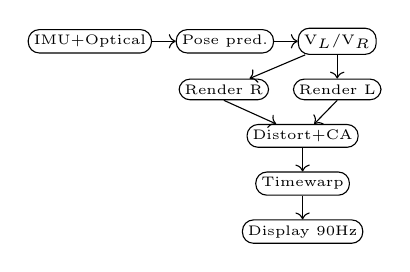
\begin{tikzpicture}[node distance=3mm and 3mm, every node/.style={font=\tiny,draw,rounded corners,inner sep=2pt}]
  \node (a) {IMU+Optical};
  \node (b) [right=of a] {Pose pred.};
  \node (c) [right=of b] {V$_L$/V$_R$};
  \node (d) [below=of c] {Render L};
  \node (e) [left=of d] {Render R};
  \node (f) [below=of e,xshift=10mm] {Distort+CA};
  \node (g) [below=of f] {Timewarp};
  \node (h) [below=of g] {Display 90Hz};
  \draw[->] (a)--(b); \draw[->] (b)--(c);
  \draw[->] (c)--(d); \draw[->] (c)--(e);
  \draw[->] (d.south)--(f); \draw[->] (e.south)--(f);
  \draw[->] (f)--(g); \draw[->] (g)--(h);
\end{tikzpicture}
\end{center}

\switchcolumn

\subsection*{1.5 Cách VR hoạt động (Pipeline)}
\textbf{Pipeline mỗi khung hình}:
\begin{enumerate}[leftmargin=*,nosep]
  \item \textbf{Lấy mẫu cảm biến}: pose của HMD (IMU + quang học) và controller.
  \item \textbf{Dự đoán}: ngoại suy pose tới thời điểm hiển thị $\Rightarrow$ giảm latency.
  \item \textbf{Cập nhật ma trận view}: dựng $V_L, V_R$ cho mắt trái/phải dùng độ lệch IPD và pose đầu.
  \item \textbf{Render lập thể}: render cảnh 2 lần (mỗi mắt 1 viewport) vào stereo target. Mỗi mắt dùng frustum lệch trục (asymmetric).
  \item \textbf{Hiệu chỉnh méo ống kính}: \emph{barrel pre-distortion} ngược chiều méo pincushion của lens; cộng thêm hiệu chỉnh sắc sai cho từng kênh R,G,B.
  \item \textbf{Reprojection / Timewarp}: ngay trước khi quét hình, warp ảnh với pose đầu mới nhất (ATW); ASW nội suy thêm khung.
  \item \textbf{Quét ra màn hình} 90/120 Hz; trộn âm thanh không gian qua HRTF.
\end{enumerate}
\textbf{Con số quan trọng}:
\begin{itemize}[leftmargin=*,nosep]
  \item Refresh $\geq$ 90 Hz mới mượt; 120 Hz tốt hơn.
  \item \textbf{Motion-to-photon latency} $<$ 20 ms (lý tưởng $<$ 11 ms) để không gây say.
  \item Phép chiếu lập thể: $\mathbf{P}_{\text{mắt}} = \mathbf{P}_{\text{proj}} \cdot \mathbf{T}(\pm \tfrac{IPD}{2}) \cdot \mathbf{V}_{\text{đầu}}$.
  \item \textbf{Foveated rendering}: chỉ render độ phân giải cao nơi mắt nhìn (cần eye-tracking), giảm 30–70\% tải GPU.
\end{itemize}

\switchcolumn*

% ---------- 1.6 AR pipeline ----------
\subsection*{1.6 How AR Works (Pipeline)}
\textbf{Generic AR pipeline}:
\begin{enumerate}[leftmargin=*,nosep]
  \item \textbf{Capture}: camera frame + IMU sample.
  \item \textbf{Pre-process}: undistort, grayscale, downsample.
  \item \textbf{Feature detection}: corners (FAST/Harris), descriptors (ORB, SIFT, SURF, BRIEF).
  \item \textbf{Tracking / pose estimation}:
    \begin{itemize}[nosep]
      \item Marker-based: detect square/QR-like marker, find 4 corners, compute homography $\mathbf{H}$, decompose to $[R|t]$ (PnP).
      \item Markerless: match features to map, run \textbf{PnP} (Perspective-n-Point) for camera pose, refine with RANSAC.
    \end{itemize}
  \item \textbf{SLAM update}: insert keyframe, triangulate new map points, run \textbf{bundle adjustment} (joint optim of poses + points).
  \item \textbf{Scene understanding}: plane detection (RANSAC on point cloud), depth from LiDAR/ToF, semantic segmentation, light estimation.
  \item \textbf{Rendering}: project virtual model with same intrinsics $K$ and pose $[R|t]$; handle \textbf{occlusion} via depth (real depth from sensor vs virtual z-buffer); composite over camera image (VST) or display via see-through.
\end{enumerate}
\textbf{Math kernels}:
\begin{itemize}[leftmargin=*,nosep]
  \item Homography $\mathbf{x'} = \mathbf{H}\mathbf{x}$ (planar), 8 DoF.
  \item Camera projection $\mathbf{x} = K[R|t]\mathbf{X}$.
  \item PnP: $\geq 3$ 3D-2D correspondences $\Rightarrow$ pose.
\end{itemize}
\textbf{SLAM variants}: ORB-SLAM (feature-based), LSD-SLAM (direct), DSO, PTAM (parallel tracking + mapping), VINS-Mono (visual-inertial), ARKit/ARCore use \textbf{VIO} (Visual-Inertial Odometry).

\begin{center}\scriptsize
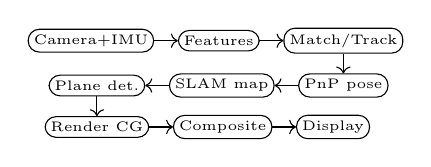
\begin{tikzpicture}[node distance=2.5mm and 3mm, every node/.style={font=\tiny,draw,rounded corners,inner sep=2pt}]
  \node (a) {Camera+IMU};
  \node (b) [right=of a] {Features};
  \node (c) [right=of b] {Match/Track};
  \node (d) [below=of c] {PnP pose};
  \node (e) [left=of d] {SLAM map};
  \node (f) [left=of e] {Plane det.};
  \node (g) [below=of f] {Render CG};
  \node (h) [right=of g] {Composite};
  \node (i) [right=of h] {Display};
  \draw[->] (a)--(b); \draw[->] (b)--(c); \draw[->] (c)--(d);
  \draw[->] (d)--(e); \draw[->] (e)--(f); \draw[->] (f)--(g);
  \draw[->] (g)--(h); \draw[->] (h)--(i);
\end{tikzpicture}
\end{center}

\switchcolumn

\subsection*{1.6 Cách AR hoạt động (Pipeline)}
\textbf{Pipeline AR tổng quát}:
\begin{enumerate}[leftmargin=*,nosep]
  \item \textbf{Chụp}: khung hình từ camera + mẫu IMU.
  \item \textbf{Tiền xử lý}: gỡ méo, chuyển xám, giảm kích thước.
  \item \textbf{Phát hiện đặc trưng}: góc (FAST/Harris), descriptor (ORB, SIFT, SURF, BRIEF).
  \item \textbf{Tracking / ước lượng pose}:
    \begin{itemize}[nosep]
      \item Marker-based: tìm marker vuông/QR, lấy 4 góc, tính homography $\mathbf{H}$, phân rã thành $[R|t]$.
      \item Markerless: khớp đặc trưng với bản đồ, chạy \textbf{PnP} để tìm pose camera, lọc bằng RANSAC.
    \end{itemize}
  \item \textbf{Cập nhật SLAM}: thêm keyframe, tam giác hóa điểm bản đồ mới, chạy \textbf{bundle adjustment}.
  \item \textbf{Hiểu cảnh}: phát hiện mặt phẳng (RANSAC trên point cloud), độ sâu từ LiDAR/ToF, segment, ước lượng ánh sáng.
  \item \textbf{Render}: chiếu mô hình ảo với cùng nội tham số $K$ và pose $[R|t]$; xử lý \textbf{occlusion} bằng độ sâu thực vs z-buffer; ghép lên ảnh camera (VST) hoặc qua optical see-through.
\end{enumerate}
\textbf{Công thức toán}:
\begin{itemize}[leftmargin=*,nosep]
  \item Homography $\mathbf{x'} = \mathbf{H}\mathbf{x}$ (mặt phẳng), 8 bậc tự do.
  \item Phép chiếu camera $\mathbf{x} = K[R|t]\mathbf{X}$.
  \item PnP: $\geq 3$ tương ứng 3D-2D $\Rightarrow$ pose.
\end{itemize}
\textbf{Biến thể SLAM}: ORB-SLAM, LSD-SLAM, DSO, PTAM, VINS-Mono; ARKit/ARCore dùng \textbf{VIO} (kết hợp camera + IMU).

\switchcolumn*

% ---------- 1.7 Tracking ----------
\subsection*{1.7 Tracking Techniques}
\begin{itemize}[leftmargin=*,nosep]
  \item \textbf{Optical}: cameras + features/markers/LEDs. High accuracy, occlusion-prone.
  \item \textbf{Inertial (IMU)}: gyroscope (angular vel.), accelerometer (linear accel), magnetometer. High frequency (1 kHz), drifts over time.
  \item \textbf{Magnetic}: tracks coil in EM field (Polhemus). Immune to occlusion, distorted by metal.
  \item \textbf{Acoustic}: ultrasonic time-of-flight. Cheap, low precision.
  \item \textbf{Mechanical}: jointed arm encoders (very precise, restricted volume).
  \item \textbf{Hybrid / Sensor fusion}: complementary filter or \textbf{Extended Kalman Filter (EKF)} fusing IMU (fast, drifts) + vision (slow, absolute) $\Rightarrow$ used in all modern HMDs.
\end{itemize}
\textbf{CV building blocks}:
\begin{itemize}[leftmargin=*,nosep]
  \item Feature detectors: Harris, FAST, DoG. Descriptors: SIFT (scale-invariant), SURF, ORB (binary, fast), BRIEF, AKAZE.
  \item Matching: brute-force / FLANN; Lowe's ratio test; RANSAC for outlier rejection.
  \item Homography (planar) vs Fundamental/Essential matrix (general epipolar geometry).
  \item Pose: solvePnP (OpenCV), Levenberg–Marquardt refinement.
\end{itemize}

\switchcolumn

\subsection*{1.7 Kỹ thuật tracking}
\begin{itemize}[leftmargin=*,nosep]
  \item \textbf{Quang học}: camera + đặc trưng/marker/LED. Chính xác cao, dễ bị che.
  \item \textbf{Quán tính (IMU)}: con quay (vận tốc góc), gia tốc kế, từ kế. Tần số cao (1 kHz) nhưng trôi theo thời gian.
  \item \textbf{Từ trường}: theo dõi cuộn dây trong từ trường (Polhemus). Không bị che nhưng méo bởi kim loại.
  \item \textbf{Âm thanh}: siêu âm đo thời gian truyền. Rẻ, kém chính xác.
  \item \textbf{Cơ học}: cánh tay khớp có encoder (cực chính xác, vùng nhỏ).
  \item \textbf{Lai / Sensor fusion}: complementary filter hoặc \textbf{Extended Kalman Filter (EKF)} kết hợp IMU + vision $\Rightarrow$ tất cả HMD hiện đại đều dùng.
\end{itemize}
\textbf{Thị giác máy tính cơ bản}:
\begin{itemize}[leftmargin=*,nosep]
  \item Phát hiện đặc trưng: Harris, FAST, DoG. Descriptor: SIFT (bất biến tỉ lệ), SURF, ORB (nhị phân, nhanh), BRIEF, AKAZE.
  \item Khớp: brute-force / FLANN; kiểm tra tỉ lệ Lowe; RANSAC loại điểm sai.
  \item Homography (mặt phẳng) vs ma trận Cơ bản/Bản chất (epipolar tổng quát).
  \item Pose: solvePnP (OpenCV), tinh chỉnh Levenberg–Marquardt.
\end{itemize}

\switchcolumn*

% ---------- 1.8 Display ----------
\subsection*{1.8 Display Technologies}
\begin{itemize}[leftmargin=*,nosep]
  \item \textbf{LCD}: cheap, full RGB sub-pixels, slower switch, backlight bleeding (Quest 2).
  \item \textbf{OLED}: deep blacks, fast response, but PenTile sub-pixel (loss of effective res), burn-in (PSVR1).
  \item \textbf{Micro-OLED (OLEDoS)}: silicon-backplane OLED, very high PPI (3000+ ppi), used in Vision Pro, Bigscreen Beyond.
  \item \textbf{LCoS / DLP}: used in projector-based AR.
  \item \textbf{Waveguides}: thin glass plates with diffraction gratings; light from micro-projector totally-internally-reflects to eye (HoloLens 2, Magic Leap).
  \item \textbf{Birdbath optics}: half-mirror combiner (Nreal/XReal Air).
  \item \textbf{Light-field displays}: multiple focal planes $\to$ correct vergence-accommodation (VAC) conflict (Magic Leap 1 had 2 planes).
  \item \textbf{Pancake lenses}: folded optics $\Rightarrow$ thinner HMD (Quest Pro/3, Vision Pro) at cost of light efficiency.
\end{itemize}
\textbf{Key metrics}:
\begin{itemize}[leftmargin=*,nosep]
  \item \textbf{FOV} (field of view): horizontal $\times$ vertical degrees. Human $\approx$ 200$^\circ$ H.
  \item \textbf{IPD} (inter-pupillary distance) 54–74 mm; mismatch $\Rightarrow$ eye strain.
  \item \textbf{PPD} (pixels per degree): retina-quality $\approx$ 60 PPD; Quest 2 $\approx$ 20, Vision Pro $\approx$ 34.
  \item \textbf{Screen-door effect (SDE)}: visible gaps between pixels.
  \item \textbf{God rays / glare}: stray light around bright objects (Fresnel lenses).
  \item \textbf{VAC}: eye \emph{vergence} (where eyes converge) vs \emph{accommodation} (focus depth) — fixed focal plane at $\sim$2 m causes conflict.
\end{itemize}

\switchcolumn

\subsection*{1.8 Công nghệ hiển thị}
\begin{itemize}[leftmargin=*,nosep]
  \item \textbf{LCD}: rẻ, sub-pixel RGB đầy đủ, chuyển chậm hơn, hở đèn nền (Quest 2).
  \item \textbf{OLED}: đen sâu, đáp ứng nhanh, nhưng PenTile làm giảm độ phân giải hiệu dụng, dễ burn-in (PSVR1).
  \item \textbf{Micro-OLED (OLEDoS)}: OLED trên đế silicon, PPI rất cao (3000+), dùng trong Vision Pro, Bigscreen Beyond.
  \item \textbf{LCoS / DLP}: dùng trong AR chiếu.
  \item \textbf{Waveguide}: tấm kính mỏng có grating; ánh sáng từ projector mini phản xạ toàn phần đến mắt (HoloLens 2, Magic Leap).
  \item \textbf{Birdbath}: gương bán phản (Nreal/XReal Air).
  \item \textbf{Light-field}: nhiều mặt tiêu cự $\to$ sửa xung đột vergence-accommodation.
  \item \textbf{Pancake lens}: thấu kính gập $\Rightarrow$ HMD mỏng hơn (Quest Pro/3, Vision Pro), đánh đổi hiệu suất sáng.
\end{itemize}
\textbf{Chỉ số quan trọng}:
\begin{itemize}[leftmargin=*,nosep]
  \item \textbf{FOV}: độ ngang $\times$ dọc. Người $\approx$ 200$^\circ$ ngang.
  \item \textbf{IPD}: 54–74 mm; sai lệch gây mỏi mắt.
  \item \textbf{PPD}: chuẩn võng mạc $\approx$ 60; Quest 2 $\approx$ 20, Vision Pro $\approx$ 34.
  \item \textbf{Screen-door effect}: thấy khe giữa các pixel.
  \item \textbf{God rays}: vệt sáng quanh vật sáng (Fresnel).
  \item \textbf{VAC}: xung đột giữa hội tụ mắt và độ nét — gây mỏi sau lâu.
\end{itemize}

\switchcolumn*

% ---------- 1.9 Software / SDK ----------
\subsection*{1.9 Software / SDKs / Tools}
\textbf{Game engines (course uses Unity)}:
\begin{itemize}[leftmargin=*,nosep]
  \item \textbf{Unity 3D}: \emph{XR Interaction Toolkit}, \emph{XR Plug-in Management}, OpenXR plug-in, AR Foundation (cross-platform AR over ARKit/ARCore).
  \item \textbf{Unreal Engine}: built-in OpenXR + ARKit/ARCore plug-ins; Niagara/MetaHuman.
  \item Godot 4 also has OpenXR.
\end{itemize}
\textbf{AR SDKs}:
\begin{itemize}[leftmargin=*,nosep]
  \item \textbf{Apple ARKit}: iOS/iPadOS; world tracking, plane detection, face/body tracking, RealityKit, LiDAR scene reconstruction.
  \item \textbf{Google ARCore}: Android; motion tracking, environmental understanding, light estimation, Geospatial API.
  \item \textbf{Vuforia}: Image targets, Model Targets, VuMarks; cross-platform, runs in Unity.
  \item \textbf{ARToolKit / ARToolKitX}: open-source fiducial-marker AR (oldest).
  \item \textbf{8th Wall, Zappar}: WebAR.
  \item \textbf{Microsoft MRTK}: Mixed Reality Toolkit for HoloLens/WMR.
  \item \textbf{Niantic Lightship}: AR cloud, persistent multiplayer.
\end{itemize}
\textbf{VR / Standards}:
\begin{itemize}[leftmargin=*,nosep]
  \item \textbf{OpenXR} (Khronos, 2019): cross-vendor API; replaces OpenVR/Oculus SDK lock-in.
  \item \textbf{OpenVR / SteamVR}: Valve's runtime.
  \item \textbf{Oculus Integration / Meta XR SDK}: Quest specific features.
  \item \textbf{WebXR Device API}: browser-based XR (Three.js, A-Frame, Babylon.js).
\end{itemize}
\textbf{3D content}: Blender, Maya, 3ds Max, ZBrush (sculpt), Substance (texture), Reality Capture / Meshroom (photogrammetry), Quill / Gravity Sketch (in-VR modeling).

\switchcolumn

\subsection*{1.9 Phần mềm / SDK / Công cụ}
\textbf{Game engine (môn học dùng Unity)}:
\begin{itemize}[leftmargin=*,nosep]
  \item \textbf{Unity 3D}: \emph{XR Interaction Toolkit}, \emph{XR Plug-in Management}, OpenXR plug-in, AR Foundation (đa nền tảng qua ARKit/ARCore).
  \item \textbf{Unreal Engine}: tích hợp OpenXR + ARKit/ARCore; Niagara, MetaHuman.
  \item Godot 4 cũng có OpenXR.
\end{itemize}
\textbf{SDK AR}:
\begin{itemize}[leftmargin=*,nosep]
  \item \textbf{Apple ARKit}: iOS/iPadOS; world tracking, plane, mặt/cơ thể, RealityKit, dựng cảnh LiDAR.
  \item \textbf{Google ARCore}: Android; motion tracking, hiểu môi trường, ước lượng sáng, Geospatial API.
  \item \textbf{Vuforia}: Image Target, Model Target, VuMark; chạy trong Unity.
  \item \textbf{ARToolKit / ARToolKitX}: AR marker mã nguồn mở, cổ nhất.
  \item \textbf{8th Wall, Zappar}: WebAR.
  \item \textbf{Microsoft MRTK}: cho HoloLens/WMR.
  \item \textbf{Niantic Lightship}: AR cloud, multiplayer bền vững.
\end{itemize}
\textbf{VR / Chuẩn}:
\begin{itemize}[leftmargin=*,nosep]
  \item \textbf{OpenXR} (Khronos, 2019): API đa nhà sản xuất.
  \item \textbf{OpenVR / SteamVR}: runtime của Valve.
  \item \textbf{Oculus / Meta XR SDK}: tính năng riêng Quest.
  \item \textbf{WebXR}: XR trên trình duyệt (Three.js, A-Frame, Babylon.js).
\end{itemize}
\textbf{Nội dung 3D}: Blender, Maya, 3ds Max, ZBrush, Substance, Reality Capture / Meshroom (photogrammetry), Quill / Gravity Sketch (vẽ trong VR).

\switchcolumn*

% ---------- 1.10 Unity steps ----------
\subsection*{1.10 Implementation in Unity (VR + AR)}
\textbf{VR project setup (XR Interaction Toolkit)}:
\begin{enumerate}[leftmargin=*,nosep]
  \item Create 3D project (URP recommended). \emph{Edit $\to$ Project Settings $\to$ XR Plug-in Management} $\to$ install, tick \textbf{OpenXR} (PC) or Oculus (Android Quest).
  \item Add Interaction Profiles in OpenXR settings (Oculus Touch, Valve Index, etc.).
  \item Install \emph{XR Interaction Toolkit} via Package Manager + Samples (Starter Assets).
  \item Replace Main Camera with \textbf{XR Origin (XR Rig)} prefab (camera offset + camera + LeftHand/RightHand controllers).
  \item Add \emph{XR Interaction Manager} to scene.
  \item Add interactables: \texttt{XRGrabInteractable} on objects, \emph{XR Ray Interactor} or \emph{Direct Interactor} on hands.
  \item \textbf{Locomotion}: add \emph{Locomotion System}, \emph{Teleportation Provider}, \emph{Continuous Move/Turn Provider}; teleport areas/anchors on floor.
  \item Build settings: Android $\to$ enable IL2CPP, ARM64, Oculus loader; deploy via adb.
\end{enumerate}
\textbf{AR project setup (AR Foundation)}:
\begin{enumerate}[leftmargin=*,nosep]
  \item Install AR Foundation + ARKit XR Plugin (iOS) and/or ARCore XR Plugin (Android).
  \item Scene: \textbf{AR Session} + \textbf{XR Origin (AR)} (with AR Camera, AR Camera Manager, AR Camera Background).
  \item Add \emph{AR Plane Manager} for plane detection, \emph{AR Raycast Manager} for hit-testing taps.
  \item Place objects: cast ray from screen tap $\to$ \texttt{ARRaycastHit} $\to$ instantiate prefab as child of trackable, optionally add \emph{AR Anchor}.
  \item Image tracking: \emph{AR Tracked Image Manager} + Reference Image Library.
  \item Face tracking (front cam): \emph{AR Face Manager}.
  \item Build: iOS Xcode (camera usage description in Info.plist) / Android (min API 24, ARCore supported).
\end{enumerate}
\textbf{Tip}: use \emph{XR Device Simulator} package to test without headset.

\switchcolumn

\subsection*{1.10 Triển khai trong Unity (VR + AR)}
\textbf{Cài VR (XR Interaction Toolkit)}:
\begin{enumerate}[leftmargin=*,nosep]
  \item Tạo project 3D (nên URP). \emph{Edit $\to$ Project Settings $\to$ XR Plug-in Management} $\to$ cài, tick \textbf{OpenXR} (PC) hoặc Oculus (Quest).
  \item Bật Interaction Profile trong OpenXR (Oculus Touch, Valve Index...).
  \item Cài \emph{XR Interaction Toolkit} qua Package Manager + Samples.
  \item Thay Main Camera bằng prefab \textbf{XR Origin (XR Rig)} (camera offset + camera + 2 controller).
  \item Thêm \emph{XR Interaction Manager} vào scene.
  \item Thêm interactable: \texttt{XRGrabInteractable} cho vật, \emph{XR Ray Interactor} hoặc \emph{Direct Interactor} cho tay.
  \item \textbf{Di chuyển}: thêm \emph{Locomotion System}, \emph{Teleportation Provider}, \emph{Continuous Move/Turn}; đặt teleport area trên sàn.
  \item Build: Android, IL2CPP, ARM64, loader Oculus, deploy bằng adb.
\end{enumerate}
\textbf{Cài AR (AR Foundation)}:
\begin{enumerate}[leftmargin=*,nosep]
  \item Cài AR Foundation + ARKit (iOS) hoặc ARCore (Android).
  \item Scene: \textbf{AR Session} + \textbf{XR Origin (AR)} (gồm AR Camera, Camera Manager, Camera Background).
  \item Thêm \emph{AR Plane Manager} để phát hiện mặt phẳng, \emph{AR Raycast Manager} để hit-test.
  \item Đặt vật: bắn ray từ điểm chạm $\to$ \texttt{ARRaycastHit} $\to$ instantiate prefab làm con của trackable, thêm \emph{AR Anchor} nếu cần neo cố định.
  \item Tracking ảnh: \emph{AR Tracked Image Manager} + Reference Image Library.
  \item Tracking khuôn mặt: \emph{AR Face Manager} (camera trước).
  \item Build: iOS (khai báo NSCameraUsageDescription) / Android (API $\geq$ 24, máy hỗ trợ ARCore).
\end{enumerate}
\textbf{Mẹo}: dùng \emph{XR Device Simulator} để test không cần kính.

\switchcolumn*

% ---------- 1.11 Challenges ----------
\subsection*{1.11 Key Challenges}
\textbf{Cybersickness / Motion sickness}:
\begin{itemize}[leftmargin=*,nosep]
  \item Causes: (1) sensory mismatch (eyes see motion, vestibular feels none) — \textbf{vection}; (2) \textbf{latency} $>$ 20 ms; (3) low frame rate / dropped frames; (4) wrong IPD; (5) bad lens distortion; (6) artificial locomotion (smooth turn).
  \item Mitigations: high refresh ($\geq$ 90 Hz), low motion-to-photon latency, \textbf{teleport} or snap-turn instead of smooth, vignette / tunneling during motion, stable horizon reference, comfort settings, fixed-rest frames (virtual nose, cockpit), proper IPD.
\end{itemize}
\textbf{AR-specific}:
\begin{itemize}[leftmargin=*,nosep]
  \item \emph{Tracking drift} accumulating over time $\Rightarrow$ loop closure, anchors, relocalization.
  \item \emph{Occlusion} of virtual by real: requires depth map (LiDAR/ToF) or learned depth.
  \item \emph{Lighting / shadow consistency}: estimate ambient light intensity + direction (ARKit Light Estimation, spherical harmonics).
  \item \emph{Registration error}: small camera–display latency $\Rightarrow$ swimming. OST-AR especially sensitive.
\end{itemize}
\textbf{Hardware / UX}:
\begin{itemize}[leftmargin=*,nosep]
  \item Battery, weight, heat, social acceptance ("glasshole"), privacy of always-on cameras, eye safety.
  \item \emph{Vergence-Accommodation Conflict}, \emph{God rays}, screen-door effect, FOV vs form-factor trade-off.
\end{itemize}

\switchcolumn

\subsection*{1.11 Thách thức chính}
\textbf{Say VR (cybersickness)}:
\begin{itemize}[leftmargin=*,nosep]
  \item Nguyên nhân: (1) lệch giác quan (mắt thấy chuyển động, tai trong không) — \textbf{vection}; (2) \textbf{latency} $>$ 20 ms; (3) FPS thấp / rớt khung; (4) sai IPD; (5) méo lens không sửa đúng; (6) di chuyển nhân tạo (smooth turn).
  \item Khắc phục: refresh $\geq$ 90 Hz, latency thấp, \textbf{teleport} hoặc snap-turn thay smooth, vignette/tunnel khi di chuyển, có chân trời ổn định, đặt IPD đúng, có khung tham chiếu (mũi ảo, cabin).
\end{itemize}
\textbf{Riêng AR}:
\begin{itemize}[leftmargin=*,nosep]
  \item \emph{Trôi tracking} theo thời gian $\Rightarrow$ loop closure, anchor, relocalization.
  \item \emph{Occlusion}: cần depth map (LiDAR/ToF) hoặc deep learning.
  \item \emph{Nhất quán ánh sáng/bóng}: ước lượng cường độ + hướng sáng (Light Estimation, spherical harmonics).
  \item \emph{Lệch đăng ký}: trễ giữa camera và hiển thị $\Rightarrow$ "trôi". OST-AR rất nhạy cảm.
\end{itemize}
\textbf{Phần cứng / UX}:
\begin{itemize}[leftmargin=*,nosep]
  \item Pin, trọng lượng, nhiệt, chấp nhận xã hội, riêng tư khi camera bật, an toàn mắt.
  \item \emph{Vergence-Accommodation Conflict}, \emph{god rays}, screen-door, đánh đổi FOV vs hình dáng.
\end{itemize}

\switchcolumn*

% ---------- 1.12 Applications ----------
\subsection*{1.12 Applications (Domains)}
\begin{itemize}[leftmargin=*,nosep]
  \item \textbf{Healthcare}: surgical training (Osso VR, FundamentalVR), \emph{AR surgical navigation} (overlay CT/MRI on patient — Brainlab), exposure therapy (PTSD, phobias), pain distraction, stroke rehab, anatomy education (HoloAnatomy, Complete Anatomy).
  \item \textbf{Education / Training}: \emph{flight simulators} (high-fidelity, FAA certified), military (squad training, JTAC), industrial (ABB welding, oil-rig safety), classroom (Labster, Google Expeditions / Arts \& Culture).
  \item \textbf{Entertainment}: gaming (Half-Life: Alyx, Beat Saber, VRChat), immersive cinema (Notes on Blindness), 360-video, location-based VR (The VOID).
  \item \textbf{Architecture / CAD / AEC}: design walkthroughs (Twinmotion, Enscape), \emph{BIM} visualization (Revit + Unity Reflect), client review.
  \item \textbf{Cultural heritage}: digital museums (\emph{eMuseum}), virtual reconstruction of ruins (Pompeii VR, Angkor Wat), eTourism, AR guides on-site.
  \item \textbf{Retail}: virtual try-on (IKEA Place, Warby Parker, Sephora), product configurators, virtual showrooms.
  \item \textbf{Real estate}: Matterport 3D tours, virtual staging.
  \item \textbf{Remote collaboration}: Spatial, Horizon Workrooms, Microsoft Mesh, immersive telepresence.
  \item \textbf{Automotive}: design review (Ford), HUD AR, driver training.
  \item \textbf{Manufacturing}: AR maintenance instructions (PTC Vuforia, Scope AR), digital twins.
\end{itemize}

\switchcolumn

\subsection*{1.12 Ứng dụng (lĩnh vực)}
\begin{itemize}[leftmargin=*,nosep]
  \item \textbf{Y tế}: huấn luyện phẫu thuật (Osso VR, FundamentalVR), \emph{điều hướng phẫu thuật AR} (chồng CT/MRI lên bệnh nhân — Brainlab), trị liệu phơi nhiễm (PTSD, ám ảnh), giảm đau, phục hồi đột quỵ, giáo dục giải phẫu (HoloAnatomy).
  \item \textbf{Giáo dục / Huấn luyện}: \emph{mô phỏng bay} (FAA chứng nhận), quân sự (huấn luyện đội hình, JTAC), công nghiệp (hàn ABB, an toàn giàn khoan), lớp học (Labster, Google Arts \& Culture).
  \item \textbf{Giải trí}: game (Half-Life: Alyx, Beat Saber, VRChat), phim immersive, 360-video, VR theo địa điểm (The VOID).
  \item \textbf{Kiến trúc / CAD / AEC}: dạo qua thiết kế (Twinmotion, Enscape), \emph{BIM} (Revit + Unity Reflect), khách hàng duyệt mẫu.
  \item \textbf{Di sản văn hóa}: bảo tàng số (\emph{eMuseum}), tái dựng phế tích (Pompeii VR, Angkor Wat), eTourism, hướng dẫn AR tại chỗ.
  \item \textbf{Bán lẻ}: thử đồ ảo (IKEA Place, Warby Parker, Sephora), cấu hình sản phẩm, showroom ảo.
  \item \textbf{Bất động sản}: tour 3D Matterport, staging ảo.
  \item \textbf{Cộng tác từ xa}: Spatial, Horizon Workrooms, Microsoft Mesh.
  \item \textbf{Ô tô}: review thiết kế (Ford), HUD AR, huấn luyện tài xế.
  \item \textbf{Sản xuất}: hướng dẫn bảo trì AR (Vuforia, Scope AR), digital twin.
\end{itemize}

\switchcolumn*

% ---------- 1.13 Tools-Techniques mapping ----------
\subsection*{1.13 Tools $\leftrightarrow$ Techniques Mapping}
{\scriptsize
\begin{tabular}{@{}p{2.1cm}p{2.6cm}p{2.4cm}@{}}
\toprule
\textbf{Application} & \textbf{Recommended Tool} & \textbf{Key Technique} \\
\midrule
Surgical training & Unity + Oculus + haptic & 6DoF tracking, force fb \\
AR surgery nav. & HoloLens + MRTK & Patient-CT registration, ICP \\
Anatomy edu. & HoloLens / Quest + MRTK / XRI & Volumetric render, hand tracking \\
Flight sim & Unreal + Varjo + motion seat & Stereo render, CAVE-like \\
Museum (eMuseum) & WebXR / Unity + ARFound. & Photogrammetry, image target \\
Heritage reconstr. & Blender + Unity + Quest & High-poly LOD, baked lighting \\
eTourism (city) & ARCore Geospatial / 8thWall & VPS, GPS+SLAM \\
BIM walk-through & Unity Reflect / Twinmotion & IFC import, VR Rig \\
Furniture try-on & ARKit + RealityKit & Plane det., PBR shading \\
Industrial maint. & Vuforia Studio / Scope AR & Model target, work-order UI \\
Education AR book & Unity + Vuforia Image Target & Marker pose, animation \\
VR exposure ther. & Unity + Quest + biosensor & Procedural anxiety scenes \\
Remote meeting & Microsoft Mesh / Spatial & Avatar lip-sync, spatial audio \\
\bottomrule
\end{tabular}}

\switchcolumn

\subsection*{1.13 Bảng mapping Công cụ $\leftrightarrow$ Kỹ thuật}
{\scriptsize
\begin{tabular}{@{}p{2.1cm}p{2.6cm}p{2.4cm}@{}}
\toprule
\textbf{Ứng dụng} & \textbf{Công cụ đề xuất} & \textbf{Kỹ thuật chính} \\
\midrule
Huấn luyện PT & Unity + Oculus + haptic & Tracking 6DoF, lực phản hồi \\
PT AR điều hướng & HoloLens + MRTK & Đăng ký CT-bệnh nhân, ICP \\
Giải phẫu học & HoloLens / Quest + MRTK / XRI & Render thể tích, hand tracking \\
Mô phỏng bay & Unreal + Varjo + ghế động & Stereo render, kiểu CAVE \\
Bảo tàng (eMuseum) & WebXR / Unity + ARFound. & Photogrammetry, image target \\
Tái dựng di sản & Blender + Unity + Quest & LOD đa cấp, bake ánh sáng \\
eTourism thành phố & ARCore Geospatial / 8thWall & VPS, GPS+SLAM \\
BIM walkthrough & Unity Reflect / Twinmotion & Import IFC, VR Rig \\
Thử đồ nội thất & ARKit + RealityKit & Plane det., shader PBR \\
Bảo trì CN & Vuforia / Scope AR & Model target, UI lệnh việc \\
Sách AR giáo dục & Unity + Vuforia Image Target & Pose marker, animation \\
VR phơi nhiễm & Unity + Quest + biosensor & Sinh cảnh lo âu thủ tục \\
Họp từ xa & Microsoft Mesh / Spatial & Avatar lip-sync, âm thanh KG \\
\bottomrule
\end{tabular}}

\switchcolumn*

% ---------- 1.14 Performance metrics ----------
\subsection*{1.14 Performance \& Evaluation Metrics}
\textbf{System metrics}:
\begin{itemize}[leftmargin=*,nosep]
  \item \textbf{Latency}: motion-to-photon $<$ 20 ms (target $<$ 11 ms). End-to-end = sensor + processing + render + scan-out.
  \item \textbf{Refresh rate}: 72 / 90 / 120 / 144 Hz.
  \item \textbf{Jitter}: temporal variation in pose estimate.
  \item \textbf{FOV}: degrees H $\times$ V (90$^\circ$ entry-level VR, 35–50$^\circ$ AR-OST).
  \item \textbf{PPD} pixels per degree; \textbf{angular resolution}.
  \item \textbf{Tracking}: positional accuracy (mm), rotational (deg), drift (cm/min), volume (m$^3$).
  \item \textbf{Frame time budget}: 90 Hz $\Rightarrow$ 11.1 ms / frame for both eyes.
\end{itemize}
\textbf{User metrics (subjective)}:
\begin{itemize}[leftmargin=*,nosep]
  \item \textbf{SSQ} (Simulator Sickness Questionnaire) — Kennedy et al. — nausea, oculomotor, disorientation sub-scales.
  \item \textbf{IPQ} (Igroup Presence Questionnaire) — spatial presence, involvement, realism.
  \item \textbf{Witmer–Singer Presence Questionnaire}.
  \item \textbf{SUS} (Slater–Usoh–Steed) presence; or System Usability Scale.
  \item \textbf{NASA-TLX} for workload.
  \item Behavioral: time-on-task, error rate, EDA / heart rate.
\end{itemize}

\switchcolumn

\subsection*{1.14 Hiệu năng \& Đánh giá}
\textbf{Đo hệ thống}:
\begin{itemize}[leftmargin=*,nosep]
  \item \textbf{Latency}: motion-to-photon $<$ 20 ms (mục tiêu $<$ 11 ms). Tổng = cảm biến + xử lý + render + scan-out.
  \item \textbf{Refresh}: 72 / 90 / 120 / 144 Hz.
  \item \textbf{Jitter}: dao động pose theo thời gian.
  \item \textbf{FOV}: H $\times$ V độ (VR cơ bản 90$^\circ$, AR-OST 35–50$^\circ$).
  \item \textbf{PPD}; độ phân giải góc.
  \item \textbf{Tracking}: chính xác vị trí (mm), góc (deg), drift (cm/phút), thể tích (m$^3$).
  \item \textbf{Ngân sách thời gian khung}: 90 Hz $\Rightarrow$ 11.1 ms/khung cho cả 2 mắt.
\end{itemize}
\textbf{Đo người dùng (chủ quan)}:
\begin{itemize}[leftmargin=*,nosep]
  \item \textbf{SSQ} — say mô phỏng (buồn nôn, thị giác, mất phương hướng).
  \item \textbf{IPQ} — presence (không gian, nhập vai, hiện thực).
  \item \textbf{Witmer–Singer PQ}.
  \item \textbf{SUS} (Slater–Usoh–Steed) presence; hoặc System Usability Scale.
  \item \textbf{NASA-TLX} đo tải nhận thức.
  \item Hành vi: thời gian, tỉ lệ lỗi, EDA / nhịp tim.
\end{itemize}

\switchcolumn*

% ---------- 1.15 Future trends ----------
\subsection*{1.15 Future Trends}
\begin{itemize}[leftmargin=*,nosep]
  \item \textbf{Foveated rendering} + eye tracking standard (Quest Pro, PSVR2, Vision Pro).
  \item \textbf{Pancake lenses} $\Rightarrow$ thinner, lighter HMD.
  \item \textbf{Varifocal / light-field displays} solve VAC.
  \item \textbf{Neural rendering}: NeRF, 3D Gaussian Splatting for photo-real scene capture and immersive replay; Instant-NGP for real-time NeRF.
  \item \textbf{AI-driven content}: text-to-3D (DreamFusion, GET3D), AI avatars, generative environments, ML-based hand/body tracking.
  \item \textbf{Passthrough MR} convergence (Quest 3, Vision Pro) — VR and AR on same device.
  \item \textbf{Metaverse / persistent worlds}: shared social VR (Horizon Worlds, VRChat, Roblox).
  \item \textbf{Cloud / edge XR rendering}: 5G + GeForce NOW-style streaming.
  \item \textbf{Brain-Computer Interfaces (BCI)}: Neuralink, Galea (EEG/EMG); thought-driven UI.
  \item \textbf{Haptics evolution}: ultrasound mid-air haptics (Ultraleap), electro-tactile.
  \item \textbf{Digital twins} of cities and factories (NVIDIA Omniverse, USD).
  \item \textbf{Standardization}: OpenXR ecosystem; \textbf{glTF} + \textbf{USD} for asset interop.
  \item \textbf{Privacy / ethics}: gaze data, biometric identification, mixed-reality bystanders.
\end{itemize}

\switchcolumn

\subsection*{1.15 Xu hướng tương lai}
\begin{itemize}[leftmargin=*,nosep]
  \item \textbf{Foveated rendering} + eye tracking thành tiêu chuẩn (Quest Pro, PSVR2, Vision Pro).
  \item \textbf{Thấu kính pancake} $\Rightarrow$ HMD mỏng nhẹ.
  \item \textbf{Varifocal / light-field} giải quyết VAC.
  \item \textbf{Neural rendering}: NeRF, 3D Gaussian Splatting cho dựng cảnh siêu thực; Instant-NGP cho NeRF thời gian thực.
  \item \textbf{Nội dung AI}: text-to-3D (DreamFusion, GET3D), avatar AI, môi trường sinh, tracking tay/cơ thể bằng ML.
  \item \textbf{MR passthrough hội tụ}: Quest 3, Vision Pro — VR và AR trên cùng thiết bị.
  \item \textbf{Metaverse / thế giới bền}: VR xã hội (Horizon Worlds, VRChat, Roblox).
  \item \textbf{Render đám mây/biên}: 5G + streaming kiểu GeForce NOW.
  \item \textbf{BCI}: Neuralink, Galea (EEG/EMG); UI điều khiển bằng suy nghĩ.
  \item \textbf{Haptic mới}: siêu âm chạm không khí (Ultraleap), điện-xúc giác.
  \item \textbf{Digital twin} của thành phố, nhà máy (NVIDIA Omniverse, USD).
  \item \textbf{Chuẩn hóa}: OpenXR; \textbf{glTF} + \textbf{USD} cho liên thông tài sản.
  \item \textbf{Riêng tư / đạo đức}: dữ liệu gaze, định danh sinh trắc, người ngoài cuộc trong MR.
\end{itemize}

\switchcolumn*

% ---------- 1.16 Quick reference ----------
\subsection*{1.16 Quick Reference Numbers}
{\scriptsize
\begin{tabular}{@{}lll@{}}
\toprule
\textbf{Quantity} & \textbf{Min OK} & \textbf{Good} \\
\midrule
Refresh rate & 72 Hz & 90–120 Hz \\
M2P latency & $<$ 20 ms & $<$ 11 ms \\
FOV (VR) & 90$^\circ$ & 110$^\circ$+ \\
FOV (AR-OST) & 30$^\circ$ & 50$^\circ$+ \\
PPD & 15 & 30–60 \\
IPD range & 60–66 mm & 55–72 mm \\
Tracking accuracy & 5 mm / 1$^\circ$ & $<$ 1 mm / 0.1$^\circ$ \\
Frame time @ 90 Hz & 11.1 ms & — \\
\bottomrule
\end{tabular}\\[2pt]
\textbf{Common abbreviations}: HMD, FOV, IPD, PPD, DoF, IMU, SLAM, VIO, VST, OST, MR, XR, ATW, ASW, VAC, SDE, SSQ, IPQ, NeRF, LiDAR, ToF, HRTF, BCI.}

\switchcolumn

\subsection*{1.16 Tham chiếu nhanh}
{\scriptsize
\begin{tabular}{@{}lll@{}}
\toprule
\textbf{Đại lượng} & \textbf{Tối thiểu} & \textbf{Tốt} \\
\midrule
Tần số quét & 72 Hz & 90–120 Hz \\
Trễ M2P & $<$ 20 ms & $<$ 11 ms \\
FOV (VR) & 90$^\circ$ & 110$^\circ$+ \\
FOV (AR-OST) & 30$^\circ$ & 50$^\circ$+ \\
PPD & 15 & 30–60 \\
Khoảng IPD & 60–66 mm & 55–72 mm \\
Độ chính xác tracking & 5 mm / 1$^\circ$ & $<$ 1 mm / 0.1$^\circ$ \\
Thời gian khung @ 90 Hz & 11.1 ms & — \\
\bottomrule
\end{tabular}\\[2pt]
\textbf{Viết tắt thường gặp}: HMD, FOV, IPD, PPD, DoF, IMU, SLAM, VIO, VST, OST, MR, XR, ATW, ASW, VAC, SDE, SSQ, IPQ, NeRF, LiDAR, ToF, HRTF, BCI.}

\end{paracol}


\vfill\hrule\vspace{4pt}

% ============================================================
% Section 2: Geometric Modeling — Bilingual EN | VI cheatsheet
% IT516 Advanced Computer Graphics — HCMIU final exam
% ============================================================

\begin{paracol}{2}

% ------------------ 2.1 Overview ------------------
\section*{2. Geometric Modeling}
\subsection*{2.1 Overview}
\textbf{Geometric modeling} = mathematical \& algorithmic representation, construction, and manipulation of 2D/3D shapes for graphics, CAD/CAM, simulation, 3D printing, VR/AR, medical imaging.

\textbf{Representations:}
\begin{itemize}[leftmargin=*,nosep]
  \item \textbf{Point cloud}: unordered set $P=\{p_i\in\mathbb{R}^3\}$. From LiDAR, photogrammetry, RGB-D. No topology.
  \item \textbf{Polygonal mesh}: vertices $V$, edges $E$, faces $F$. Triangle (most common, planar, GPU friendly), quad (subdivision/animation), $n$-gon. Euler: $V-E+F=2-2g$ ($g$=genus). \emph{Manifold}: every edge incident to $\le 2$ faces; vertex link is a disk/half-disk. \emph{Watertight}=closed manifold (no boundary).
  \item \textbf{Parametric surfaces}: $S(u,v)=\sum B_i(u)B_j(v)P_{ij}$. Bezier, B-spline, NURBS. Smooth, exact, but harder to render directly.
  \item \textbf{Implicit / level sets}: zero-set $\{x:f(x)=0\}$. SDF (signed distance field), metaballs. Easy boolean ops, free topology change.
  \item \textbf{Volumetric / voxels}: 3D grid $V_{ijk}$. CT/MRI, sparse octree, OpenVDB. High memory.
  \item \textbf{CSG (Constructive Solid Geometry)}: tree of $\cup,\cap,\setminus$ on primitives.
  \item \textbf{Subdivision surfaces}: Catmull-Clark, Loop, Doo-Sabin — refine coarse mesh to smooth limit.
\end{itemize}

\textbf{Pipeline:} acquisition $\to$ registration/alignment $\to$ denoising/outlier removal $\to$ surface reconstruction (triangulation) $\to$ hole filling/repair $\to$ simplification/remeshing $\to$ parameterization/UV $\to$ analysis (curvature, geodesics) $\to$ rendering / export.

\textbf{File formats:}
\begin{itemize}[leftmargin=*,nosep]
  \item \textbf{OBJ} (Wavefront): ASCII, \texttt{v}/\texttt{vn}/\texttt{vt}/\texttt{f}, no topology guarantee.
  \item \textbf{PLY} (Stanford): ASCII or binary, header-driven, supports per-vertex color/normal/custom attrs.
  \item \textbf{STL}: triangles only, no shared vertices, used for 3D printing.
  \item \textbf{OFF}: simple ASCII (vertex count, face count, then data).
  \item \textbf{FBX} (Autodesk): rigging, animation, materials.
  \item \textbf{DAE} (COLLADA): XML, exchange format.
  \item \textbf{glTF/GLB}: web/runtime, PBR materials.
\end{itemize}

\switchcolumn

\section*{2. Mô hình hình học}
\subsection*{2.1 Tổng quan}
\textbf{Geometric modeling} = biểu diễn và xử lý toán học/thuật toán cho hình dạng 2D/3D, dùng trong đồ họa, CAD/CAM, mô phỏng, in 3D, VR/AR, ảnh y khoa.

\textbf{Các dạng biểu diễn:}
\begin{itemize}[leftmargin=*,nosep]
  \item \textbf{Đám mây điểm (point cloud)}: tập điểm rời rạc $P=\{p_i\}$. Từ LiDAR, photogrammetry, RGB-D. Không có topology.
  \item \textbf{Lưới đa giác (mesh)}: đỉnh $V$, cạnh $E$, mặt $F$. Tam giác phổ biến nhất; quad cho subdivision/animation. Euler: $V-E+F=2-2g$. \emph{Manifold}: mỗi cạnh $\le 2$ mặt kề; link đỉnh là đĩa. \emph{Watertight}=manifold kín, không biên.
  \item \textbf{Mặt tham số}: Bezier, B-spline, NURBS — mượt, chính xác, khó render trực tiếp.
  \item \textbf{Implicit/level set}: $\{x:f(x)=0\}$. SDF, metaballs. Dễ phép boolean, đổi topology tự do.
  \item \textbf{Voxel/khối}: lưới 3D, dùng CT/MRI, octree, OpenVDB. Tốn bộ nhớ.
  \item \textbf{CSG}: cây boolean $\cup,\cap,\setminus$ trên các khối nguyên thủy.
  \item \textbf{Subdivision}: Catmull-Clark, Loop, Doo-Sabin — tinh chỉnh lưới thô thành mặt mượt.
\end{itemize}

\textbf{Pipeline:} thu nhận $\to$ căn chỉnh (registration) $\to$ khử nhiễu/loại outlier $\to$ tái tạo bề mặt (triangulation) $\to$ lấp lỗ/sửa lưới $\to$ đơn giản hóa/remesh $\to$ tham số hóa UV $\to$ phân tích (độ cong, geodesic) $\to$ render/xuất.

\textbf{Định dạng file:}
\begin{itemize}[leftmargin=*,nosep]
  \item \textbf{OBJ}: ASCII, dòng \texttt{v}/\texttt{vn}/\texttt{vt}/\texttt{f}.
  \item \textbf{PLY}: ASCII hoặc nhị phân, header linh hoạt, hỗ trợ thuộc tính tùy biến.
  \item \textbf{STL}: chỉ tam giác, không chia sẻ đỉnh, in 3D.
  \item \textbf{OFF}: ASCII đơn giản.
  \item \textbf{FBX}: rigging, animation.
  \item \textbf{DAE}: XML, format trao đổi.
  \item \textbf{glTF/GLB}: chuẩn web/runtime, vật liệu PBR.
\end{itemize}

\switchcolumn*

% ------------------ 2.2 Mesh Simplification ------------------
\subsection*{2.2 Mesh Simplification}
\textbf{Goal}: reduce triangle count $|F|$ from $N\to N'\!\ll\!N$ while preserving shape, attributes (UV, color, normal), and topology where possible.

\textbf{Algorithms:}
\begin{enumerate}[leftmargin=*,nosep]
  \item \textbf{Vertex clustering} (Rossignac \& Borrel 1993). Overlay 3D grid; collapse all vertices in each cell to one representative (centroid or quadric-optimal). $O(N)$, very fast, low quality, topology may change. Used as out-of-core preprocess.
  \item \textbf{Vertex decimation} (Schroeder 1992). Iteratively remove "removable" vertices (classified by curvature/feature angle), retriangulate hole. Keeps subset of original vertices.
  \item \textbf{Edge collapse + Quadric Error Metric (QEM)} (Garland \& Heckbert 1997). Most popular, high quality. \emph{Math:}
    \begin{itemize}[leftmargin=1.2em,nosep]
      \item Each face has plane $\pi=(a,b,c,d)^T$ with $a^2+b^2+c^2=1$. Squared distance from $v=(x,y,z,1)^T$ to plane: $(\pi^T v)^2 = v^T(\pi\pi^T)v$.
      \item Per-vertex \emph{quadric} $Q_v = \sum_{\pi\in\text{planes}(v)} \pi\pi^T$ (a $4{\times}4$ symmetric PSD).
      \item Cost of collapsing edge $(v_i,v_j)\to\bar v$: $E(\bar v)=\bar v^T(Q_i+Q_j)\bar v$.
      \item Optimal $\bar v$: solve $\partial E/\partial \bar v=0$, i.e., set top $3\times4$ block of $Q_i+Q_j$ to identity-target; if invertible, $\bar v=Q'^{-1}(0,0,0,1)^T$. Else fall back to midpoint or endpoint with minimum $E$.
      \item Maintain min-heap keyed on $E$; pop, collapse, update neighbors' quadrics ($Q_{\bar v}=Q_i+Q_j$) and edge costs.
    \end{itemize}
  \item \textbf{Progressive meshes} (Hoppe 1996). Store base mesh $M^0$ + sequence of vertex splits $\{vs_i\}$ enabling continuous LOD, streaming, geomorph.
  \item \textbf{Edge collapse with attribute quadrics} (extended QEM): augment $Q$ to handle color, UV, normals as extra dims.
\end{enumerate}

\textbf{Quality metrics:}
\begin{itemize}[leftmargin=*,nosep]
  \item \textbf{Hausdorff distance}: $d_H(A,B)=\max(\sup_{a\in A}\inf_{b\in B}\|a-b\|,\,\sup_b\inf_a\|a-b\|)$.
  \item \textbf{RMS error}: $\sqrt{\tfrac{1}{|A|}\int_A d(a,B)^2 dA}$ — Metro tool (Cignoni 1998).
  \item Normal angle deviation, visual fidelity (perceptual).
\end{itemize}

\textbf{Applications}: real-time rendering LOD, network streaming, mobile/VR, collision proxy, mip-map of geometry.

\switchcolumn

\subsection*{2.2 Đơn giản hóa lưới}
\textbf{Mục tiêu}: giảm số tam giác $|F|$ trong khi giữ hình dạng, thuộc tính (UV, màu, pháp tuyến), và topology.

\textbf{Thuật toán:}
\begin{enumerate}[leftmargin=*,nosep]
  \item \textbf{Vertex clustering} (Rossignac \& Borrel 1993). Phủ lưới 3D grid; mọi đỉnh trong cùng cell gộp làm một (centroid hoặc QEM-optimal). $O(N)$, rất nhanh, chất lượng thấp, có thể đổi topology. Hữu dụng tiền xử lý dữ liệu lớn.
  \item \textbf{Vertex decimation} (Schroeder 1992). Lặp xóa các đỉnh "có thể xóa" (đánh giá theo độ cong, góc đặc trưng), tam giác hóa lại lỗ. Giữ tập con đỉnh gốc.
  \item \textbf{Edge collapse + QEM} (Garland \& Heckbert 1997). Phổ biến nhất, chất lượng cao.
    \begin{itemize}[leftmargin=1.2em,nosep]
      \item Mỗi mặt có mặt phẳng $\pi=(a,b,c,d)^T$, $a^2+b^2+c^2=1$. Khoảng cách bình phương từ $v$ đến $\pi$: $(\pi^T v)^2 = v^T(\pi\pi^T)v$.
      \item Quadric mỗi đỉnh: $Q_v=\sum_\pi \pi\pi^T$ ($4{\times}4$ đối xứng PSD).
      \item Chi phí gộp cạnh $(v_i,v_j)\to\bar v$: $E(\bar v)=\bar v^T(Q_i+Q_j)\bar v$.
      \item Tối ưu $\bar v$ bằng giải $\partial E/\partial \bar v=0$; nếu suy biến dùng trung điểm.
      \item Heap nhỏ nhất theo $E$; pop, collapse, cập nhật $Q$ và chi phí lân cận.
    \end{itemize}
  \item \textbf{Progressive meshes} (Hoppe 1996). Lưu mesh gốc $M^0$ và chuỗi vertex split, hỗ trợ LOD liên tục, streaming, geomorph.
  \item \textbf{QEM mở rộng}: $Q$ có thêm dimension cho màu/UV/normal.
\end{enumerate}

\textbf{Đo chất lượng:}
\begin{itemize}[leftmargin=*,nosep]
  \item \textbf{Hausdorff}: $d_H(A,B)=\max(\sup\inf,\sup\inf)$.
  \item \textbf{RMS}: căn quân phương khoảng cách (Metro tool).
  \item Lệch normal, đánh giá thị giác.
\end{itemize}

\textbf{Ứng dụng}: LOD real-time, streaming mạng, mobile/VR, collision proxy, mip-map hình học.

\switchcolumn*

% ------------------ 2.3 Triangulation ------------------
\subsection*{2.3 Triangulation (Point Cloud $\to$ Mesh)}

\textbf{Delaunay triangulation (DT)}:
\begin{itemize}[leftmargin=*,nosep]
  \item \emph{Definition (empty-circle property)}: triangulation $T$ of $P\subset\mathbb{R}^2$ is Delaunay iff for every triangle, its circumcircle contains no other point of $P$ in its interior. 3D: empty circumsphere.
  \item \emph{Optimality}: maximizes the minimum angle $\Rightarrow$ avoids slivers (best in lex-order of angle vectors). Unique if no 4 cocircular points.
  \item \emph{Dual} of \textbf{Voronoi diagram}: $V_i=\{x:\|x-p_i\|\le\|x-p_j\|\forall j\}$. Connect $p_i,p_j$ iff their Voronoi cells share an edge.
  \item \emph{Complexity (2D)}: $O(N\log N)$.
  \item \emph{Algorithms}:
    \begin{itemize}[leftmargin=1em,nosep]
      \item \textbf{Incremental insertion + edge flip} (Lawson). Insert point, locate triangle, split into 3, flip non-Delaunay edges (use in-circle test).
      \item \textbf{Bowyer–Watson} (incremental, dual view, see pseudocode).
      \item \textbf{Divide \& Conquer} (Guibas \& Stolfi) $O(N\log N)$.
      \item \textbf{Sweep-line} (Fortune, primarily Voronoi).
    \end{itemize}
  \item \emph{In-circle predicate} for triangle $abc$ and query $d$ (CCW): $d$ is inside circumcircle iff
  \[\det\!\begin{pmatrix}a_x{-}d_x & a_y{-}d_y & \|a{-}d\|^2\\ b_x{-}d_x & b_y{-}d_y & \|b{-}d\|^2\\ c_x{-}d_x & c_y{-}d_y & \|c{-}d\|^2\end{pmatrix}>0.\]
\end{itemize}

\textbf{Bowyer–Watson algorithm:}

\begin{algorithm}[H]
\scriptsize
\SetAlgoLined
\KwIn{Points $P$}
\KwOut{Delaunay triangulation $T$}
$T \leftarrow \{$super-triangle containing all $P\}$\;
\ForEach{point $p\in P$}{
  $\mathcal{B} \leftarrow \{t\in T :\, p\in \text{circumcircle}(t)\}$ \tcp*{bad triangles}
  $\mathcal{P} \leftarrow$ boundary edges of $\mathcal{B}$ that are not shared by two bad triangles \tcp*{polygon hole}
  $T \leftarrow T \setminus \mathcal{B}$\;
  \ForEach{edge $e \in \mathcal{P}$}{
    add triangle formed by $e$ and $p$ to $T$\;
  }
}
remove all triangles touching the super-triangle\;
\Return $T$\;
\caption{Bowyer–Watson Delaunay}
\end{algorithm}

\textbf{Constrained Delaunay (CDT)}: enforce specified edges; relaxation: edge $(u,v)$ is locally Delaunay if no constrained edge separates $u,v$ from a fourth point. Used in GIS, mesh generation.

\textbf{3D point-cloud surface reconstruction:}
\begin{itemize}[leftmargin=*,nosep]
  \item \textbf{Ball Pivoting Algorithm (BPA)} (Bernardini 1999). Pivot a ball of radius $\rho$ around boundary edges; whenever it touches three points without containing any others, form triangle. Sensitive to $\rho$ vs sampling density. $O(N\log N)$ with KD-tree.
  \item \textbf{Poisson Surface Reconstruction} (Kazhdan, Bolitho, Hoppe 2006). Treat oriented points as samples of a vector field $\vec V$ approximating gradient of indicator function $\chi$; solve $\nabla\!\cdot\!\nabla\chi=\nabla\!\cdot\!\vec V$ on octree, extract iso-surface via Marching Cubes. Smooth, watertight, robust to noise. \emph{Screened Poisson} (2013) adds point-fitting term.
  \item \textbf{$\alpha$-shapes} (Edelsbrunner). Generalization of convex hull: from DT keep simplices with circumradius $\le\alpha$. $\alpha\!\to\!\infty$: convex hull; $\alpha\!\to\!0$: just points.
  \item \textbf{Marching Cubes} (Lorensen \& Cline 1987). For implicit/scalar volume: per cube of 8 corners, sign pattern indexes into 256-entry lookup table (15 base cases by symmetry); produce 0–4 triangles. Linearly interpolate iso-vertex on edges. \emph{Marching Tetrahedra} avoids ambiguities.
  \item \textbf{Greedy Projection Triangulation} (Marton, PCL). Project local neighborhood to tangent plane (from PCA normal), incrementally grow front by adding triangles that meet angle/edge-length thresholds.
  \item \textbf{Convex hull / Gift wrap / QuickHull}: only for convex point sets. 3D QuickHull is $O(N\log N)$ avg.
  \item \textbf{Crust / Cocone} (Amenta, Bern, Dey): theoretically guaranteed reconstruction from $\epsilon$-sampled smooth surfaces, uses DT and Voronoi poles.
\end{itemize}

\switchcolumn

\subsection*{2.3 Tam giác hóa (Point Cloud $\to$ Lưới)}

\textbf{Delaunay triangulation (DT)}:
\begin{itemize}[leftmargin=*,nosep]
  \item \emph{Định nghĩa (vòng tròn rỗng)}: tam giác hóa $T$ của $P\subset\mathbb{R}^2$ là Delaunay khi mỗi tam giác có vòng ngoại tiếp không chứa điểm khác bên trong. 3D: hình cầu ngoại tiếp rỗng.
  \item \emph{Tính tối ưu}: cực đại góc nhỏ nhất $\Rightarrow$ tránh tam giác "lưỡi dao". Duy nhất nếu không có 4 điểm đồng viên.
  \item \emph{Đối ngẫu của \textbf{Voronoi}}: cell $V_i=\{x:\|x-p_i\|\le\|x-p_j\|\}$; nối $p_i,p_j$ nếu cell chia cạnh.
  \item Độ phức tạp 2D: $O(N\log N)$.
  \item Thuật toán:
    \begin{itemize}[leftmargin=1em,nosep]
      \item \textbf{Incremental + edge flip} (Lawson): chèn điểm, định vị, chia 3 tam giác, flip cạnh không Delaunay (in-circle test).
      \item \textbf{Bowyer–Watson} (incremental).
      \item \textbf{Chia để trị} $O(N\log N)$.
      \item \textbf{Sweep-line} (Fortune, chủ yếu cho Voronoi).
    \end{itemize}
  \item \emph{Phép thử in-circle} cho $abc,d$ (CCW): định thức $3\times3$ với cột là lệch tọa độ và bình phương khoảng cách; $>0\Leftrightarrow d$ trong vòng ngoại tiếp.
\end{itemize}

\textbf{Bowyer–Watson:} (xem pseudocode bên cột tiếng Anh)
\begin{enumerate}[leftmargin=*,nosep]
  \item Khởi tạo $T$ với super-triangle bao toàn bộ $P$.
  \item Với mỗi $p$: tìm tam giác "xấu" có $p$ trong vòng ngoại tiếp; lấy biên đa giác từ chúng; xóa và nối lại với $p$.
  \item Cuối cùng xóa tam giác kề super-triangle.
\end{enumerate}

\textbf{Constrained Delaunay (CDT)}: ép giữ các cạnh chỉ định; locally Delaunay khi không có cạnh constraint chia cách. Dùng trong GIS, sinh lưới.

\textbf{Tái tạo bề mặt từ point cloud 3D:}
\begin{itemize}[leftmargin=*,nosep]
  \item \textbf{Ball Pivoting (BPA)} (Bernardini 1999): lăn quả bóng bán kính $\rho$ quanh cạnh biên; khi chạm 3 điểm mà không chứa điểm khác $\to$ tạo tam giác. Phải chọn $\rho$ phù hợp mật độ.
  \item \textbf{Poisson Reconstruction} (Kazhdan 2006): coi điểm có normal là gradient của hàm chỉ thị $\chi$; giải $\nabla\!\cdot\!\nabla\chi = \nabla\!\cdot\!\vec V$ trên octree, trích iso-surface bằng Marching Cubes. Mượt, watertight, kháng nhiễu. \emph{Screened Poisson} (2013) thêm constraint khớp điểm.
  \item \textbf{$\alpha$-shapes}: tổng quát hóa bao lồi; từ DT giữ simplex có bán kính ngoại tiếp $\le\alpha$.
  \item \textbf{Marching Cubes} (1987): mỗi cube 8 góc, dấu các góc index vào bảng 256 (15 case cơ bản); sinh 0–4 tam giác, nội suy tuyến tính trên cạnh. \emph{Marching Tetrahedra} tránh ambiguity.
  \item \textbf{Greedy Projection} (PCL/Marton): chiếu vùng lân cận lên mặt phẳng tiếp tuyến, mở rộng front theo ngưỡng góc/độ dài.
  \item \textbf{Convex hull} (QuickHull 3D): chỉ với tập lồi.
  \item \textbf{Crust / Cocone} (Amenta): có đảm bảo lý thuyết với $\epsilon$-sampling từ mặt mượt; dùng Voronoi poles.
\end{itemize}

\switchcolumn*

% ------------------ 2.4 Hole Filling ------------------
\subsection*{2.4 Hole Filling}

\textbf{Boundary detection (manifold mesh)}:
\begin{itemize}[leftmargin=*,nosep]
  \item Half-edge with no twin / edge with exactly 1 incident face $\Rightarrow$ \emph{boundary edge}.
  \item Walk boundary edges to extract \emph{boundary loops} (each hole = one loop).
  \item Algorithm: pick unmarked boundary edge; from its end vertex, follow next boundary edge around the umbrella until back to start.
\end{itemize}

\textbf{Hole filling families:}
\begin{itemize}[leftmargin=*,nosep]
  \item \textbf{Liepa (2003)}: classic 3-stage triangulation–refinement–fairing.
    \begin{enumerate}[leftmargin=1.2em,nosep]
      \item \emph{Min-weight triangulation} of boundary loop. Weight $w(t){=}(\text{area},\text{dihedral})$ lex. DP: $W(i,j){=}\min_{i<m<j} W(i,m){+}W(m,j){+}w(\triangle v_iv_mv_j)$, $O(n^3)$.
      \item \emph{Refinement}: subdivide patch triangles whose edge length far from surrounding density (relax via centroid-split + edge swap).
      \item \emph{Fairing}: minimize membrane/thin-plate energy via Laplacian/biharmonic smoothing on patch interior, boundary fixed.
    \end{enumerate}
  \item \textbf{Advancing front}: start at boundary, repeatedly add best triangle (smallest angle / closest pair) until front closes.
  \item \textbf{RBF-based} (Carr, Branch \& Olague): fit radial basis function $\phi(\|x-x_i\|)$ on boundary points + normals, evaluate iso-surface to plug hole. Smooth, $C^\infty$, expensive globally.
  \item \textbf{Poisson hole filling} (Zhao, Gao, Lin 2007): solve Poisson equation for vertex positions over patch.
  \item \textbf{Volumetric} (Curless \& Levoy 1996): rasterize mesh to SDF in voxel grid, diffuse/extend SDF into hole, extract surface via Marching Cubes. Robust but loses detail.
  \item \textbf{Context-based / template-based} (Sharf, Pauly, Bischoff): search the mesh for self-similar patches and copy.
  \item \textbf{MLS-based} (Jun 2005): moving least squares fit on boundary normals/positions.
\end{itemize}

\textbf{NFD — Normal Field Diffusion} (user's project, MeshLab plugin):
\begin{enumerate}[leftmargin=*,nosep]
  \item \textbf{Step 1 — Hole detection}: find boundary loops by walking border half-edges; each loop $L_h$ stored as ordered vertex indices, validated by size $3\le|L_h|\le$ \texttt{MaxHoleSize}.
  \item \textbf{Step 2 — Boundary analysis}: for each boundary vertex, compute \emph{normal} (area-weighted from one-ring) and \emph{discrete mean curvature}.
  \item \textbf{Step 3 — Initial triangulation}: build local frame from average boundary normal $\bar{\mathbf n}=\sum \mathbf n_i/\|\cdot\|$, project boundary loop to 2D plane $(u,v)$, triangulate (2D Delaunay/ear-clipping), insert interior Steiner vertices on a regular grid; lift back to 3D as flat patch.
  \item \textbf{Step 4 — Normal field diffusion (CORE)}: solve heat equation on patch graph for each component $k\in\{x,y,z\}$ of normal,
    $\partial n_k/\partial t = \Delta n_k$, Dirichlet BC $n_k|_{\partial\Omega}=n_{k,\text{fix}}$.
    Discretize with cotangent Laplacian $L_{ij}=\tfrac12(\cot\alpha_{ij}+\cot\beta_{ij})$ and \emph{implicit Euler}: $(I-\lambda L)\mathbf n_k^{t+1}=\mathbf n_k^t$. Cholesky/$LDL^T$ via Eigen \texttt{SimplicialLDLT}; unconditionally stable. Re-normalize $\|\mathbf n\|=1$ per vertex after iterations.
  \item \textbf{Step 5 — Laplacian smoothing of positions} (uniform, boundary fixed) — 3 iters to even spacing.
  \item \textbf{Step 6 — Curvature-guided displacement (spherical-cap)}:
    \begin{itemize}[leftmargin=1em,nosep]
      \item Estimate cap height $h$ from boundary geometry: $h = R(1-\cos\bar\theta)$ with $R$ = mean boundary distance to centroid, $\bar\theta = \mathrm{avg}_i\arccos(\mathbf n_i\!\cdot\!\bar{\mathbf n})$ (average is more robust than max).
      \item Geodesic distance $d_i$ from boundary via Dijkstra (multi-source); normalize $t_i = d_i/\max d_j\in[0,1]$.
      \item Weight profile $w(t)=\sqrt{2t-t^2}$ (spherical cap, $w(0)=0,w(1)=1$, $w'(0)=\infty\Rightarrow C^1$ at boundary).
      \item Displace: $v_i' = v_i + h\,w(t_i)\,\mathbf n_i^{\text{diffused}}$ (per-vertex direction $\Rightarrow$ patch follows local curvature).
    \end{itemize}
  \item \textbf{Step 7 — Patch merging}: re-index boundary to original mesh vertices (no duplicates), add interior vertices/faces, average colors from neighborhood for visual continuity. Optional Taubin $(\lambda,\mu)=(0.40,-0.44)$ to remove spikes.
\end{enumerate}

\textbf{Quality criteria:} continuity ($C^0$ position match, $C^1$ tangent match, $C^2$ curvature match), smoothness (low Dirichlet/bending energy), no self-intersection, feature preservation.

\textbf{Challenges}: complex hole topology (islands, multiply-connected), sharp features, large holes, non-manifold input, mesh with handles.

\switchcolumn

\subsection*{2.4 Lấp lỗ (Hole Filling)}

\textbf{Phát hiện biên (mesh manifold)}:
\begin{itemize}[leftmargin=*,nosep]
  \item Half-edge không có twin / cạnh có đúng 1 mặt $\Rightarrow$ cạnh biên.
  \item Đi vòng các cạnh biên để trích boundary loop (mỗi lỗ = 1 loop).
  \item Thuật toán: chọn cạnh biên chưa đánh dấu; từ đỉnh cuối, đi cạnh biên tiếp theo trong umbrella đến khi quay lại.
\end{itemize}

\textbf{Các họ thuật toán:}
\begin{itemize}[leftmargin=*,nosep]
  \item \textbf{Liepa (2003)}: ba giai đoạn.
    \begin{enumerate}[leftmargin=1.2em,nosep]
      \item \emph{Min-weight triangulation} loop biên: trọng số (diện tích, góc dihedral) thứ tự lex; DP $O(n^3)$ với $W(i,j)=\min_m W(i,m)+W(m,j)+w(\triangle)$.
      \item \emph{Refinement}: chia nhỏ tam giác có cạnh quá lớn so với mật độ xung quanh.
      \item \emph{Fairing}: tối thiểu năng lượng màng/uốn bằng Laplacian/biharmonic, biên cố định.
    \end{enumerate}
  \item \textbf{Advancing front}: từ biên, lặp thêm tam giác tốt nhất (góc nhỏ nhất / cặp gần nhất) đến khi front đóng.
  \item \textbf{RBF}: khớp $\phi(\|x-x_i\|)$ trên điểm/normal biên, lấy iso-surface; mượt $C^\infty$.
  \item \textbf{Poisson}: giải Poisson cho vị trí đỉnh trên patch.
  \item \textbf{Volumetric} (Curless–Levoy 1996): rasterize SDF trên voxel grid, diffuse SDF vào lỗ, Marching Cubes. Chắc chắn, mất chi tiết.
  \item \textbf{Template/context-based}: tìm patch tự tương tự trên mesh và sao chép.
  \item \textbf{MLS} (Jun 2005): moving least squares trên normal/vị trí biên.
\end{itemize}

\textbf{NFD — Normal Field Diffusion} (project của bạn, plugin MeshLab):
\begin{enumerate}[leftmargin=*,nosep]
  \item \textbf{Bước 1 — Phát hiện lỗ}: đi vòng border half-edge; mỗi loop là dãy chỉ số đỉnh, kiểm tra $3\le|L_h|\le$ \texttt{MaxHoleSize}.
  \item \textbf{Bước 2 — Phân tích biên}: tính normal (area-weighted một-vòng) và mean curvature rời rạc cho từng đỉnh biên.
  \item \textbf{Bước 3 — Tam giác hóa khởi tạo}: dựng frame từ $\bar{\mathbf n}=\sum\mathbf n_i/\|\cdot\|$, chiếu loop xuống 2D, tam giác hóa (Delaunay/ear-clip), thêm Steiner trong lưới đều, nâng lên 3D thành patch phẳng.
  \item \textbf{Bước 4 — Normal Field Diffusion (LÕI)}: giải heat equation $\partial n_k/\partial t = \Delta n_k$ (mỗi component $k$), Dirichlet $n_k|_{\partial\Omega}$ cố định. Rời rạc bằng cotangent Laplacian $L_{ij}=\tfrac12(\cot\alpha+\cot\beta)$, \emph{implicit Euler}: $(I-\lambda L)\mathbf n^{t+1}=\mathbf n^t$. Cholesky $LDL^T$ qua Eigen \texttt{SimplicialLDLT}; ổn định vô điều kiện. Chuẩn hóa $\|\mathbf n\|=1$.
  \item \textbf{Bước 5 — Laplacian smoothing vị trí} (uniform, biên cố định, 3 iter) để đều khoảng cách.
  \item \textbf{Bước 6 — Dịch chuyển theo độ cong (chỏm cầu)}:
    \begin{itemize}[leftmargin=1em,nosep]
      \item Cao độ vòm $h=R(1-\cos\bar\theta)$, $R$ = bán kính trung bình từ centroid, $\bar\theta=$ trung bình $\arccos(\mathbf n_i\cdot\bar{\mathbf n})$ (trung bình bền hơn max).
      \item Khoảng cách geodesic $d_i$ từ biên (Dijkstra multi-source), chuẩn hóa $t_i=d_i/\max d_j$.
      \item Trọng số $w(t)=\sqrt{2t-t^2}$ (chỏm cầu, $w(0)=0$, $w'(0)=\infty$ $\Rightarrow$ $C^1$ ở biên).
      \item Dịch chuyển: $v_i' = v_i + h\,w(t_i)\,\mathbf n_i^{\text{diffused}}$.
    \end{itemize}
  \item \textbf{Bước 7 — Ghép patch}: tái-index biên về đỉnh gốc của mesh (không tạo trùng), thêm đỉnh/mặt nội bộ, lấy màu trung bình lân cận. Tùy chọn Taubin $(\lambda,\mu)=(0.40,-0.44)$ để khử gai.
\end{enumerate}

\textbf{Tiêu chí chất lượng:} liên tục $C^0/C^1/C^2$, mượt (Dirichlet/bending energy thấp), không tự cắt, giữ chi tiết.

\textbf{Thách thức}: lỗ topology phức tạp (đảo, đa liên thông), chi tiết sắc, lỗ lớn, mesh không manifold, mesh có quai.

\switchcolumn*

% ------------------ 2.5 Noise Removal ------------------
\subsection*{2.5 Noise Removal / Mesh \& Point Cloud Denoising}

\textbf{Sources of noise}: scanner sensor noise (Kinect $\sigma\!\sim\!$ mm), registration misalignment, photogrammetry artifacts, quantization, reconstruction artifacts.

\textbf{Mesh smoothing:}
\begin{itemize}[leftmargin=*,nosep]
  \item \textbf{Uniform Laplacian}: $\mathbf v_i^{(k+1)} = \mathbf v_i^{(k)} + \lambda L(\mathbf v_i)$, $L(\mathbf v_i) = \tfrac{1}{|N(i)|}\sum_{j\in N(i)}(\mathbf v_j - \mathbf v_i)$. Causes \emph{shrinkage} (volume loss) and over-smoothing of features.
  \item \textbf{Cotangent Laplacian} (more accurate, conformal): $L(\mathbf v_i) = \tfrac{1}{2A_i}\sum_j(\cot\alpha_{ij}+\cot\beta_{ij})(\mathbf v_j-\mathbf v_i)$, $A_i$ = Voronoi area. Discretizes mean curvature: $\Delta\mathbf v = -2H\mathbf n$.
  \item \textbf{Taubin $\lambda|\mu$ smoothing} (1995): alternate $\lambda>0$ shrink and $\mu<-\lambda<0$ inflate, $|\mu|>\lambda$. Ideally $\tfrac{1}{\lambda}+\tfrac{1}{\mu}=k_{pb}$ (pass-band) keeps low-freq, kills high-freq. Eliminates shrinkage.
  \item \textbf{Bilateral mesh denoising} (Fleishman 2003 / Jones 2003): per vertex $v$ with normal $\mathbf n$, neighbors $\{q_i\}$:
    $$\hat v = v + \mathbf n \cdot \frac{\sum_i w_c(\|q_i-v\|)\,w_s(\langle\mathbf n,q_i-v\rangle)\,\langle\mathbf n,q_i-v\rangle}{\sum_i w_c\,w_s}$$
    where $w_c(d)=e^{-d^2/2\sigma_c^2}$ (spatial), $w_s(h)=e^{-h^2/2\sigma_s^2}$ (signal). Edge-preserving (anisotropic).
  \item \textbf{Mean curvature flow}: $\partial \mathbf x/\partial t = -H\,\mathbf n$. Implicit (Desbrun 1999): $(I-\lambda L_{cot})\mathbf x^{t+1}=\mathbf x^t$ — unconditionally stable.
  \item \textbf{Anisotropic diffusion} (Desbrun, Hildebrandt): diffusion coefficient depends on local feature ($\to 0$ near sharp edges).
  \item \textbf{Bilateral normal filter} (Zheng 2011): smooth normals first, then update positions to match.
  \item \textbf{$L_0$ mesh smoothing} (He \& Schaefer 2013): minimize $\sum_e \|D(e)\|_0$ — preserves planar regions, sharp edges.
  \item \textbf{Robust statistics}: replace mean by median in Laplacian for outlier resilience.
\end{itemize}

\textbf{Point cloud denoising:}
\begin{itemize}[leftmargin=*,nosep]
  \item \textbf{Statistical Outlier Removal (SOR)} (PCL): for each point compute mean distance $\mu_i$ to its $k$ nearest neighbors; global $\mu=\mathrm{avg}(\mu_i)$, $\sigma=\mathrm{std}(\mu_i)$; remove $p_i$ if $\mu_i>\mu+\alpha\sigma$ (typical $k=20,\alpha=1.0$).
  \item \textbf{Radius outlier removal}: discard point with $<n_{\min}$ neighbors within radius $r$.
  \item \textbf{Voxel-grid downsampling}: replace points in each voxel by centroid (uniform density).
  \item \textbf{Moving Least Squares (MLS)} (Levin, Alexa): fit local polynomial $g(u,v)$ on tangent plane (PCA), project point onto $g$. Smooths and resamples.
  \item \textbf{WLOP (Weighted Locally Optimal Projection)} (Huang 2009): iteratively project points to a clean, evenly distributed set; minimizes attraction $\sum\|x_i-p_j\|\theta(\cdot)$ + repulsion.
  \item \textbf{PCA normal estimation}: covariance of $k$-NN, smallest eigenvalue's eigenvector $=$ normal; sign disambiguated by Riemannian propagation (MST).
  \item \textbf{Bilateral point cloud filter}: similar to mesh bilateral but on neighborhoods.
  \item \textbf{RIMLS} (Robust Implicit MLS, Öztireli 2009): robust kernel (Geman-McClure) preserves features.
  \item \textbf{Learning-based}: PointCleanNet, Total Denoising, score-based diffusion (Luo \& Hu 2021).
\end{itemize}

\textbf{Edge-preserving} = bilateral, anisotropic, $L_0$, RIMLS.

\textbf{Quality measures}: Hausdorff distance, RMS-to-ground-truth, normal angle error $\arccos(\hat{\mathbf n}\!\cdot\!\mathbf n_{gt})$, feature preservation (chamfer on edge sets).

\switchcolumn

\subsection*{2.5 Khử nhiễu lưới và point cloud}

\textbf{Nguồn nhiễu}: cảm biến scanner (Kinect $\sigma\sim$ mm), lệch registration, photogrammetry, lượng tử hóa, artifact tái tạo.

\textbf{Smoothing trên mesh:}
\begin{itemize}[leftmargin=*,nosep]
  \item \textbf{Laplacian đều}: $\mathbf v_i^{(k+1)} = \mathbf v_i^{(k)}+\lambda L(\mathbf v_i)$, $L(\mathbf v_i)=\tfrac{1}{|N(i)|}\sum(\mathbf v_j-\mathbf v_i)$. Gây \emph{co rút} thể tích, làm mòn chi tiết.
  \item \textbf{Cotangent Laplacian}: $L(\mathbf v_i)=\tfrac{1}{2A_i}\sum(\cot\alpha+\cot\beta)(\mathbf v_j-\mathbf v_i)$, $A_i$ = diện tích Voronoi. Rời rạc mean curvature: $\Delta\mathbf v=-2H\mathbf n$.
  \item \textbf{Taubin $\lambda|\mu$}: xen kẽ $\lambda>0$ (co) và $\mu<-\lambda$ (giãn). Điều kiện $|\mu|>\lambda$. Pass-band $\tfrac1\lambda+\tfrac1\mu=k_{pb}$. Tránh co rút.
  \item \textbf{Bilateral mesh denoising} (Fleishman/Jones 2003): với $v$ có normal $\mathbf n$,
    $\hat v = v + \mathbf n\cdot \tfrac{\sum w_c\,w_s\,\langle\mathbf n,q_i-v\rangle}{\sum w_c\,w_s}$,
    $w_c=$ Gaussian không gian, $w_s=$ Gaussian tín hiệu — bảo toàn cạnh.
  \item \textbf{Mean curvature flow}: $\partial\mathbf x/\partial t = -H\mathbf n$. Implicit (Desbrun 1999): $(I-\lambda L_{cot})\mathbf x^{t+1}=\mathbf x^t$, ổn định vô điều kiện.
  \item \textbf{Khuếch tán bất đẳng hướng}: hệ số khuếch tán nhỏ ở cạnh sắc.
  \item \textbf{Bilateral normal filter} (Zheng 2011): mượt normal trước, cập nhật vị trí khớp.
  \item \textbf{$L_0$ smoothing} (He–Schaefer 2013): tối thiểu $\|D(e)\|_0$, giữ vùng phẳng và cạnh.
  \item \textbf{Thống kê bền}: dùng median thay mean để chống outlier.
\end{itemize}

\textbf{Khử nhiễu point cloud:}
\begin{itemize}[leftmargin=*,nosep]
  \item \textbf{SOR}: tính $\mu_i$ = trung bình khoảng cách đến $k$-NN; loại $p_i$ nếu $\mu_i>\mu+\alpha\sigma$ (thường $k=20,\alpha=1.0$).
  \item \textbf{Radius outlier}: loại điểm có $<n_{\min}$ neighbor trong bán kính $r$.
  \item \textbf{Voxel downsampling}: thay điểm trong mỗi voxel bằng centroid.
  \item \textbf{MLS} (Levin): khớp đa thức cục bộ trên mặt phẳng tiếp tuyến (PCA), chiếu điểm.
  \item \textbf{WLOP} (Huang 2009): chiếu điểm đến tập sạch và phân bố đều, kết hợp lực hút và đẩy.
  \item \textbf{PCA normal}: hiệp phương sai $k$-NN, eigenvector của giá trị riêng nhỏ nhất là normal; định hướng nhất quán bằng MST.
  \item \textbf{Bilateral} cho point cloud.
  \item \textbf{RIMLS} (Öztireli 2009): kernel bền (Geman-McClure) giữ chi tiết.
  \item \textbf{Học máy}: PointCleanNet, score-based (Luo \& Hu 2021).
\end{itemize}

\textbf{Bảo toàn cạnh} = bilateral, anisotropic, $L_0$, RIMLS.

\textbf{Đo chất lượng}: Hausdorff, RMS so với ground-truth, sai số góc normal, chamfer trên tập cạnh.

\switchcolumn*

% ------------------ 2.6 Worked example ------------------
\subsection*{2.6 Worked Example}

\textbf{(A) QEM edge collapse on 4-vertex tetra-fan.}\\
Vertices $v_1=(0,0,0), v_2=(1,0,0), v_3=(0,1,0), v_4=(1,1,0), v_5=(0.5,0.5,1)$. Faces all share $v_5$ apex on a square base.

\emph{Step 1.} Plane of base face $v_1v_2v_3$: normal $(0,0,1)$, $d=0$, so $\pi=(0,0,1,0)^T$, $\pi\pi^T=\mathrm{diag}(0,0,1,0)$.

\emph{Step 2.} Compute $Q_i=\sum_{\pi\in F(i)}\pi\pi^T$ for each vertex. For base vertices, $Q_i$ accumulates plane $z=0$ once + side planes.

\emph{Step 3.} Candidate edge $(v_1,v_2)$. $Q_{12}=Q_1+Q_2$. Solve $\partial(\bar v^TQ_{12}\bar v)/\partial\bar v=0$ by setting top $3\times4$ rows of $Q_{12}$ replaced as $[I\,|\,0]$ targeted to $(0,0,0,1)^T$. If singular fall back: try midpoint $(0.5,0,0)$ and endpoints, pick min $E$. Suppose $E_{mid}=0.012$ is smallest. Push $(v_1,v_2,0.012,(0.5,0,0))$ to heap. Repeat for all edges; pop min, collapse, update incident $Q$'s.

\textbf{(B) Bowyer–Watson on 4 points} $A=(0,0),B=(2,0),C=(2,2),D=(1,1)$.

\emph{Init} super-triangle $S$ enclosing all (e.g., huge $(-100,-100)$, $(100,-100)$, $(0,100)$). $T=\{S\}$.

\emph{Insert $A$:} $S$ contains $A$ in circumcircle (yes); bad=$\{S\}$, polygon = 3 edges of $S$; new $T = \{SA_1,SA_2,SA_3\}$ (three triangles around $A$).

\emph{Insert $B$:} Find triangles whose circumcircle contains $B$ (some subset). Remove, retriangulate hole boundary fan around $B$.

\emph{Insert $C$:} similar.

\emph{Insert $D$:} $D=(1,1)$ may lie inside circumcircle of $\triangle ABC$ (yes, since $ABC$ is right-isoceles with circumcircle through them; check: circumcenter of $A,B,C=(1,1)$, radius $=\sqrt 2$; $D$ at center is inside) so $\triangle ABC$ is bad; remove, retriangulate cavity into $\triangle ABD,\triangle BCD,\triangle CAD$.

\emph{Cleanup:} delete every triangle touching a super-triangle vertex. Final DT $=\{ABD,BCD,CAD\}$ (the unique DT of these 4 points if no 4 cocircular, else flip-equivalent).

\textbf{(C) Laplacian smoothing — 5-vertex umbrella.} Center $v_0=(0,0,1)$, ring $v_1\!=\!(1,0,0),v_2\!=\!(0,1,0),v_3\!=\!(-1,0,0),v_4\!=\!(0,-1,0)$. Uniform Laplacian on $v_0$:
$L(v_0)=\tfrac14\sum(v_i-v_0)=\tfrac14(0,0,-4)=(0,0,-1)$.
With $\lambda=0.5$: $v_0' = (0,0,1)+0.5\cdot(0,0,-1)=(0,0,0.5)$ — moved halfway toward ring centroid. Repeat $\to$ shrinkage.

To prevent shrinkage, follow with Taubin $\mu=-0.53$: $v_0'' = v_0' + (-0.53)\cdot L(v_0')$. Recompute $L(v_0')=\tfrac14\sum(v_i-v_0')=\tfrac14(0,0,-2)=(0,0,-0.5)$, so $v_0''=(0,0,0.5)+(-0.53)(0,0,-0.5)=(0,0,0.765)$ — partially restored.

\switchcolumn

\subsection*{2.6 Ví dụ tính toán}

\textbf{(A) QEM edge collapse trên fan 5 đỉnh.}\\
Đỉnh: $v_1\!=\!(0,0,0)$, $v_2\!=\!(1,0,0)$, $v_3\!=\!(0,1,0)$, $v_4\!=\!(1,1,0)$, đỉnh chóp $v_5=(0.5,0.5,1)$.

\emph{B1.} Mặt phẳng đáy có normal $(0,0,1)$, $\pi=(0,0,1,0)$, $\pi\pi^T=\mathrm{diag}(0,0,1,0)$.

\emph{B2.} $Q_i=\sum_{\pi\in F(i)}\pi\pi^T$ cộng dồn các mặt kề.

\emph{B3.} Cạnh $(v_1,v_2)$: $Q_{12}=Q_1+Q_2$. Giải $\nabla(\bar v^T Q_{12}\bar v)=0$. Nếu suy biến, thử trung điểm $(0.5,0,0)$ và hai endpoint, chọn $E$ nhỏ nhất. Đẩy vào heap; pop nhỏ nhất; collapse; cập nhật $Q$ các đỉnh kề.

\textbf{(B) Bowyer–Watson 4 điểm} $A=(0,0),B=(2,0),C=(2,2),D=(1,1)$.

\emph{Init:} super-triangle $S$ rất lớn bao toàn bộ. $T=\{S\}$.

\emph{Chèn $A$:} $S$ có $A$ trong vòng ngoại tiếp; bad=$\{S\}$; xóa $S$, tạo 3 tam giác từ 3 cạnh $S$ với $A$.

\emph{Chèn $B$, $C$:} tương tự.

\emph{Chèn $D=(1,1)$:} $\triangle ABC$ có tâm $(1,1)$, bán kính $\sqrt2$, $D$ ở chính tâm $\Rightarrow$ trong vòng. $\triangle ABC$ bad; xóa, lấp khoang bằng $\triangle ABD,\triangle BCD,\triangle CAD$.

\emph{Cleanup:} xóa tam giác kề super vertex. DT cuối cùng: $\{ABD,BCD,CAD\}$.

\textbf{(C) Laplacian smoothing — umbrella 5 đỉnh.}\\ Tâm $v_0{=}(0,0,1)$; vòng $(1,0,0)$, $(0,1,0)$, $({-}1,0,0)$, $(0,{-}1,0)$.

$L(v_0)=\tfrac14\sum(v_i-v_0)=(0,0,-1)$.
Với $\lambda=0.5$: $v_0'=(0,0,0.5)$ — di chuyển nửa đường về centroid vòng (co rút).

Bù bằng Taubin $\mu=-0.53$: $L(v_0')=(0,0,-0.5)$; $v_0''=(0,0,0.5)+(-0.53)(0,0,-0.5)=(0,0,0.765)$ — phục hồi một phần.

\switchcolumn*

% ------------------ 2.7 Reference Table ------------------
\subsection*{2.7 Quick Reference Table}

\scriptsize
\setlength{\tabcolsep}{2pt}
\begin{tabular}{@{}p{2.4cm}p{1.4cm}p{1.5cm}p{1.5cm}p{1.9cm}p{2.2cm}@{}}
\toprule
\textbf{Algorithm} & \textbf{Input} & \textbf{Output} & \textbf{Cmplx.} & \textbf{Key param.} & \textbf{When to use} \\
\midrule
Vertex clustering & mesh & coarse mesh & $O(N)$ & grid cell size & out-of-core, fast LOD \\
Vertex decimation & mesh & coarse mesh & $O(N\log N)$ & feature angle & moderate quality \\
QEM edge collapse & mesh & coarse mesh & $O(N\log N)$ heap & target \#faces & best quality LOD \\
Progressive mesh & mesh & PM stream & $O(N\log N)$ & — & streaming, geomorph \\
Delaunay (B-W) & 2D points & DT & $O(N\log N)$ avg & — & quality 2D mesh \\
Constrained DT & pts + edges & CDT & $O((N+k)\log N)$ & constraint set & GIS, FEM domain \\
Ball Pivoting & oriented pts & mesh & $O(N\log N)$ & ball radius $\rho$ & uniform-density scan \\
Poisson Recon & oriented pts & watertight mesh & $O(N\log N)$ octree & depth $d$, samp/node & noisy scans \\
$\alpha$-shapes & 3D pts & mesh & $O(N^2)$ 3D & $\alpha$ & coarse hull family \\
Marching Cubes & scalar volume & mesh & $O(K^3)$ & iso-value & SDF/volume data \\
Greedy proj. tri. & oriented pts & mesh & $O(N\log N)$ & search radius, ang. & PCL pipeline \\
Liepa hole fill & hole loop & patch & $O(n^3)$ DP & weight $(A,\theta)$ & generic small holes \\
Advancing front & loop & patch & $O(n^2)$ & angle threshold & moderate holes \\
RBF fill & loop\,+\,nrm & patch & $O(n^3)$ solve & kernel $\phi$ & smooth $C^\infty$ \\
Volumetric fill & mesh & repaired mesh & $O(K^3)$ voxels & voxel size & topology fix \\
NFD hole fill & mesh+hole & patch & $O(n)$ Cholesky & $\lambda,$ iters & curvature-aware \\
Uniform Laplacian & mesh & smoothed & $O(N)$/iter & $\lambda$, iter & quick smooth \\
Cotangent Lap. & mesh & smoothed & $O(N)$/iter & $\lambda$, iter & accurate, conformal \\
Taubin $\lambda|\mu$ & mesh & smoothed & $O(N)$/iter & $\lambda,\mu$ & no shrink \\
Bilateral mesh & mesh & smoothed & $O(Nk)$ & $\sigma_c,\sigma_s$ & feature-preserving \\
Mean curv. flow & mesh & smoothed & solve/iter & step $\Delta t$ & PDE smoothing \\
$L_0$ smoothing & mesh & smoothed & ADMM iters & $\beta$ & sharp-edge cleanup \\
SOR & point cloud & cleaner & $O(Nk)$ kNN & $k,\alpha$ & remove outliers \\
Radius outlier & pts & cleaner & $O(N)$ kdtree & $r,n_{\min}$ & sparse outliers \\
Voxel grid & pts & down\-sampled & $O(N)$ & voxel size & uniform resamp. \\
MLS proj. & pts & smooth pts & $O(Nk)$ & poly. deg & smooth+resamp \\
WLOP & pts & even pts & iterative & $h,\mu$ & even distribution \\
PCA normal est. & pts & normals & $O(Nk)$ & $k$ & normal init for recon \\
RIMLS & pts & smooth pts & iter & robust $\sigma_r$ & feature preserving \\
\bottomrule
\end{tabular}
\normalsize

\switchcolumn

\subsection*{2.7 Bảng tham chiếu nhanh}

\scriptsize
\setlength{\tabcolsep}{2pt}
\begin{tabular}{@{}p{2.4cm}p{1.4cm}p{1.5cm}p{1.5cm}p{1.9cm}p{2.2cm}@{}}
\toprule
\textbf{Thuật toán} & \textbf{Đầu vào} & \textbf{Đầu ra} & \textbf{Phức tạp} & \textbf{T.số chính} & \textbf{Khi nào dùng} \\
\midrule
Vertex clustering & mesh & mesh thô & $O(N)$ & cỡ ô grid & LOD nhanh, dữ liệu lớn \\
Vertex decimation & mesh & mesh thô & $O(N\log N)$ & góc đặc trưng & chất lượng vừa \\
QEM collapse & mesh & mesh thô & $O(N\log N)$ heap & số face đích & LOD chất lượng cao \\
Progressive mesh & mesh & PM & $O(N\log N)$ & — & streaming, geomorph \\
Delaunay (B-W) & điểm 2D & DT & $O(N\log N)$ & — & lưới 2D chất lượng \\
CDT & điểm + cạnh & CDT & $O((N+k)\log N)$ & tập constraint & GIS, FEM \\
Ball Pivoting & điểm + normal & mesh & $O(N\log N)$ & bán kính $\rho$ & scan đều mật độ \\
Poisson Recon & điểm + normal & mesh kín & $O(N\log N)$ & depth, samp/node & scan nhiễu \\
$\alpha$-shapes & điểm 3D & mesh & $O(N^2)$ & $\alpha$ & họ bao thô \\
Marching Cubes & volume & mesh & $O(K^3)$ & iso-value & SDF/volume \\
Greedy proj. & điểm + normal & mesh & $O(N\log N)$ & bán kính, góc & pipeline PCL \\
Liepa fill & loop biên & patch & $O(n^3)$ DP & $(A,\theta)$ & lỗ nhỏ tổng quát \\
Advancing front & loop & patch & $O(n^2)$ & ngưỡng góc & lỗ vừa \\
RBF fill & loop\,+\,nrm & patch & $O(n^3)$ & kernel $\phi$ & lỗ mượt $C^\infty$ \\
Volumetric fill & mesh & mesh sửa & $O(K^3)$ voxel & cỡ voxel & sửa topology \\
NFD fill & mesh+lỗ & patch & $O(n)$ Cholesky & $\lambda$, số iter & lỗ theo độ cong \\
Laplacian đều & mesh & mượt & $O(N)$/iter & $\lambda$, iter & smooth nhanh \\
Cotangent Lap. & mesh & mượt & $O(N)$/iter & $\lambda$, iter & chính xác, conformal \\
Taubin $\lambda|\mu$ & mesh & mượt & $O(N)$/iter & $\lambda,\mu$ & không co rút \\
Bilateral mesh & mesh & mượt & $O(Nk)$ & $\sigma_c,\sigma_s$ & giữ cạnh \\
Mean curv. flow & mesh & mượt & solve/iter & $\Delta t$ & smooth PDE \\
$L_0$ smoothing & mesh & mượt & ADMM & $\beta$ & dọn cạnh sắc \\
SOR & point cloud & sạch hơn & $O(Nk)$ & $k,\alpha$ & loại outlier \\
Radius outlier & điểm & sạch hơn & $O(N)$ kdtree & $r,n_{\min}$ & outlier rời rạc \\
Voxel grid & điểm & down\-sample & $O(N)$ & cỡ voxel & lấy mẫu đều \\
MLS proj. & điểm & mượt & $O(Nk)$ & bậc đa thức & smooth+resamp \\
WLOP & điểm & đều & lặp & $h,\mu$ & phân bố đều \\
PCA normal & điểm & normal & $O(Nk)$ & $k$ & init normal \\
RIMLS & điểm & mượt & lặp & $\sigma_r$ bền & giữ chi tiết \\
\bottomrule
\end{tabular}
\normalsize

\switchcolumn*

% ------------------ 2.8 Memory aids ------------------
\subsection*{2.8 Memory Aids / Pitfalls}
\begin{itemize}[leftmargin=*,nosep]
  \item \emph{Cotangent weights} can be \emph{negative} on obtuse triangles $\to$ matrix loses M-property, possible flips. Mitigate via intrinsic Delaunay.
  \item \emph{Implicit Euler} for diffusion: stable for any $\Delta t$ but each step needs sparse solve; precompute Cholesky factor once if topology fixed.
  \item \emph{QEM optimal $\bar v$}: always check matrix invertibility; degenerate $\Rightarrow$ midpoint fallback.
  \item \emph{Hole detection on non-manifold} edges: an edge with $\ge 3$ incident faces is non-manifold, not a hole; pre-clean.
  \item \emph{Marching Cubes ambiguity}: face/internal ambiguity $\Rightarrow$ cracks; use asymptotic decider or Marching Tetrahedra.
  \item \emph{Taubin}: requires $|\mu|>\lambda$; if $\mu=-\lambda$ pass-band $k_{pb}=0$ no smoothing.
  \item \emph{Laplacian} on irregular mesh = uniform $\ne$ cotangent; uniform behaves like graph diffusion (curvature flow only on regular meshes).
  \item \emph{Hausdorff} is asymmetric in general; use 2-sided $\max$.
  \item \emph{Poisson recon} blurs sharp features (low-pass); try \emph{screened} variant or feature-aware methods.
  \item \emph{Boundary loops $\ne$ holes 1-1} when surface has multiple holes sharing topology (e.g., torus with bites).
\end{itemize}

\switchcolumn

\subsection*{2.8 Mẹo nhớ / Bẫy thường gặp}
\begin{itemize}[leftmargin=*,nosep]
  \item Trọng số \emph{cotangent} có thể âm trên tam giác tù $\Rightarrow$ ma trận mất M-property, có thể flip. Khắc phục bằng intrinsic Delaunay.
  \item \emph{Implicit Euler} ổn định mọi $\Delta t$ nhưng mỗi bước phải solve sparse; precompute Cholesky nếu topology cố định.
  \item \emph{QEM} $\bar v$ tối ưu: luôn kiểm tra suy biến; nếu suy biến dùng trung điểm.
  \item Phát hiện lỗ trên mesh không manifold: cạnh có $\ge 3$ mặt là non-manifold, không phải lỗ; cần dọn trước.
  \item \emph{Marching Cubes ambiguity}: face/internal $\Rightarrow$ lỗ rạn; dùng asymptotic decider hoặc MT.
  \item \emph{Taubin} cần $|\mu|>\lambda$; nếu $\mu=-\lambda$ thì pass-band $k_{pb}=0$, không smooth.
  \item Laplacian đều $\ne$ cotangent trên mesh không đều; uniform = graph diffusion.
  \item \emph{Hausdorff} bất đối xứng; nên dùng max hai chiều.
  \item \emph{Poisson recon} làm mờ chi tiết sắc; dùng \emph{screened} hoặc feature-aware.
  \item Boundary loop $\ne$ lỗ 1-1 khi topology phức (ví dụ torus bị cắn).
\end{itemize}

\end{paracol}


\vfill\hrule\vspace{4pt}

% =====================================================================
% Section 3 — Medical Image Processing (Bilingual EN | VI)
% =====================================================================
\begin{paracol}{2}

% ---------------------------------------------------------------------
% 3.1 Imaging Modalities
% ---------------------------------------------------------------------
\section*{3. Medical Image Processing}
\subsection*{3.1 Imaging Modalities}
\textbf{MRI (Magnetic Resonance Imaging).}
\begin{itemize}[leftmargin=*,nosep]
  \item \emph{Physics:} hydrogen ($^1$H) protons in water/fat align with strong static field $B_0$ (1.5T or 3T). RF pulse at Larmor freq.\ $\omega_0=\gamma B_0$ tips magnetization; gradient coils ($G_x,G_y,G_z$) encode space; receive coil samples FID.
  \item \emph{Relaxation:} $T_1$ longitudinal recovery, $T_2$ transverse decay, $T_2^*$ (with field inhomogeneity), PD (proton density).
  \item \emph{Sequences:} T1w, T2w, FLAIR (fluid-attenuated, suppresses CSF), DWI (diffusion), MRA (angiography), fMRI BOLD (blood oxygen level dependent), MRS (spectroscopy), SWI.
  \item \emph{Strengths:} excellent soft-tissue contrast; no ionizing radiation; multiplanar.
  \item \emph{Weaknesses:} slow ($\sim$30 min), expensive, claustrophobia, contraindication with metal/pacemakers.
  \item \emph{Output:} k-space (Fourier domain) $\to$ DICOM volume.
\end{itemize}

\textbf{CT (Computed Tomography).}
\begin{itemize}[leftmargin=*,nosep]
  \item \emph{Physics:} rotating X-ray source + arc detector; multi-angle line integrals of attenuation $\mu(x,y)$ form sinogram $p(t,\theta)$.
  \item \emph{Reconstruction:} Filtered Back Projection (FBP) using Radon inverse; or iterative (ART, SIRT, MLEM, MBIR), now deep-learning recon.
  \item \emph{Hounsfield Units:} $\mathrm{HU}=1000\frac{\mu-\mu_w}{\mu_w}$. Air $-1000$, fat $-100$, water $0$, soft tissue $-100..+100$, bone $+400..+1000$, metal $>+2000$.
  \item Fast ($<$1\,s/slice), high spatial resolution, but ionizing.
  \item CT angiography (CTA), perfusion CT, dual-energy CT, cone-beam CT (CBCT).
\end{itemize}

\textbf{Ultrasound (US).}
\begin{itemize}[leftmargin=*,nosep]
  \item Piezoelectric transducer emits 2--15 MHz pulses; echo time $\to$ depth $d=ct/2$ ($c\!\approx\!1540$ m/s in soft tissue).
  \item Modes: A-mode (1D amplitude), B-mode (2D brightness), M-mode (motion), Doppler (flow velocity via freq shift).
  \item Real-time, cheap, no radiation, portable; operator-dependent, poor through bone/air. Use: obstetrics, cardiac (echo), abdominal, vascular.
\end{itemize}

\textbf{PET (Positron Emission Tomography).}
\begin{itemize}[leftmargin=*,nosep]
  \item Radiotracer ($^{18}$F-FDG, $^{11}$C, $^{68}$Ga) emits $\beta^+$; positron annihilates with electron $\to$ pair of 511\,keV $\gamma$ photons at $\sim$180$^\circ$; ring detectors record coincidences.
  \item Functional/metabolic imaging (glucose uptake $\Rightarrow$ tumor activity).
  \item Hybrid PET-CT and PET-MRI co-register anatomy + function.
\end{itemize}

\textbf{X-ray (planar radiography, mammography).} 2D projection of attenuation; cheap; bone/lung screening; mammography uses low-energy X-ray for breast soft tissue.

\textbf{Other modalities (brief).}
\begin{itemize}[leftmargin=*,nosep]
  \item \textbf{SPECT:} $\gamma$-emitting tracer (Tc-99m); cheaper than PET, lower res.
  \item \textbf{OCT:} optical coherence tomography, low-coherence interferometry, micrometer resolution; ophthalmology, dermatology.
  \item \textbf{Fluoroscopy:} continuous X-ray for real-time guidance (catheter, GI).
  \item \textbf{Endoscopy, microscopy (H\&E, IHC) — pathology.}
\end{itemize}

\textbf{DICOM (Digital Imaging and Communications in Medicine).}
File = header (tag-VR-length-value triples: PatientID, Modality, PixelSpacing, SliceThickness, RescaleIntercept/Slope, StudyUID, SeriesUID, SOPInstanceUID) + pixel data. Network protocol DIMSE. PACS (Picture Archive and Communication System) stores; HL7/FHIR for textual records.

\smallskip
\footnotesize
\begin{tabular}{@{}llllll@{}}
\toprule
Mod. & Physics & Res. & Rad. & Speed & Best for \\
\midrule
MRI & H+RF+B$_0$ & $\sim$1 mm & no & slow & soft tissue, brain \\
CT & X-ray & $<$0.5 mm & yes & fast & bone, lung, trauma \\
US & sound echo & $\sim$0.5 mm & no & real-time & OB, cardiac \\
PET & $\beta^+$ tracer & $\sim$4 mm & yes & medium & metabolism, oncology \\
X-ray & X-ray 2D & $\sim$0.1 mm & yes & instant & chest, bone, mammo \\
SPECT & $\gamma$ tracer & $\sim$8 mm & yes & medium & cardiac, bone scan \\
OCT & near-IR light & $\mu$m & no & fast & retina, skin \\
\bottomrule
\end{tabular}
\normalsize

\switchcolumn

\section*{3. Xử lý ảnh y tế}
\subsection*{3.1 Phương thức tạo ảnh}
\textbf{MRI (Cộng hưởng từ).}
\begin{itemize}[leftmargin=*,nosep]
  \item \emph{Vật lý:} proton $^1$H trong nước/mỡ xếp theo từ trường tĩnh $B_0$ (1.5T hoặc 3T). Xung RF tại tần số Larmor $\omega_0=\gamma B_0$ làm lệch từ hóa; cuộn gradient $G_x,G_y,G_z$ mã hóa không gian; cuộn thu nhận tín hiệu FID.
  \item \emph{Hồi phục:} $T_1$ dọc, $T_2$ ngang, $T_2^*$ (kèm bất đồng nhất từ trường), PD (mật độ proton).
  \item \emph{Chuỗi xung:} T1w, T2w, FLAIR (xóa dịch não tủy), DWI (khuếch tán), MRA (mạch máu), fMRI BOLD (oxy hóa máu), MRS (phổ), SWI.
  \item \emph{Ưu:} tương phản mô mềm xuất sắc; không bức xạ ion hóa; đa mặt phẳng.
  \item \emph{Nhược:} chậm ($\sim$30 phút), đắt, sợ kín, chống chỉ định với kim loại/máy tạo nhịp.
  \item \emph{Đầu ra:} k-space (miền Fourier) $\to$ thể tích DICOM.
\end{itemize}

\textbf{CT (Cắt lớp vi tính).}
\begin{itemize}[leftmargin=*,nosep]
  \item \emph{Vật lý:} ống X-quang quay + dãy đầu dò; tích phân đường suy giảm $\mu(x,y)$ ở nhiều góc $\to$ sinogram $p(t,\theta)$.
  \item \emph{Tái tạo:} Filtered Back Projection (FBP) qua biến đổi Radon ngược; hoặc lặp (ART, SIRT, MLEM, MBIR), nay có deep-learning recon.
  \item \emph{Hounsfield Unit:} $\mathrm{HU}=1000\frac{\mu-\mu_w}{\mu_w}$. Khí $-1000$, mỡ $-100$, nước $0$, mô mềm $-100..+100$, xương $+400..+1000$, kim loại $>+2000$.
  \item Nhanh ($<$1\,s/lát), độ phân giải cao, nhưng có bức xạ.
  \item CT mạch máu (CTA), CT tưới máu, CT đa năng lượng, CBCT (cone-beam).
\end{itemize}

\textbf{Siêu âm (US).}
\begin{itemize}[leftmargin=*,nosep]
  \item Đầu dò áp điện phát xung 2--15 MHz; thời gian dội $\to$ độ sâu $d=ct/2$ ($c\!\approx\!1540$ m/s trong mô mềm).
  \item Chế độ: A-mode (biên độ 1D), B-mode (sáng 2D), M-mode (chuyển động), Doppler (vận tốc dòng theo dịch chuyển tần số).
  \item Thời gian thực, rẻ, không bức xạ, di động; phụ thuộc kỹ thuật viên, kém qua xương/khí. Dùng: sản phụ khoa, tim mạch, ổ bụng, mạch máu.
\end{itemize}

\textbf{PET (Cắt lớp phát xạ positron).}
\begin{itemize}[leftmargin=*,nosep]
  \item Chất đánh dấu phóng xạ ($^{18}$F-FDG, $^{11}$C, $^{68}$Ga) phát $\beta^+$; positron hủy với electron $\to$ cặp photon $\gamma$ 511\,keV cách nhau $\sim$180$^\circ$; vòng đầu dò ghi nhận trùng hợp.
  \item Hình ảnh chức năng/chuyển hóa (hấp thu glucose $\Rightarrow$ hoạt động khối u).
  \item PET-CT và PET-MRI lai ghép giải phẫu + chức năng.
\end{itemize}

\textbf{X-quang (chụp phẳng, chụp nhũ ảnh).} Hình chiếu 2D của hệ số suy giảm; rẻ; tầm soát xương/phổi; nhũ ảnh dùng X-quang năng lượng thấp cho mô mềm vú.

\textbf{Các phương thức khác (tóm tắt).}
\begin{itemize}[leftmargin=*,nosep]
  \item \textbf{SPECT:} chất đánh dấu phát $\gamma$ (Tc-99m); rẻ hơn PET, độ phân giải kém hơn.
  \item \textbf{OCT:} chụp cắt lớp quang học giao thoa độ kết hợp thấp, độ phân giải micromet; nhãn khoa, da liễu.
  \item \textbf{Soi huỳnh quang (Fluoroscopy):} X-quang liên tục thời gian thực (đặt catheter, tiêu hóa).
  \item \textbf{Nội soi, kính hiển vi (H\&E, IHC) — giải phẫu bệnh.}
\end{itemize}

\textbf{DICOM.}
File = header (bộ ba tag-VR-length-value: PatientID, Modality, PixelSpacing, SliceThickness, RescaleIntercept/Slope, StudyUID, SeriesUID, SOPInstanceUID) + dữ liệu pixel. Giao thức mạng DIMSE. PACS lưu trữ; HL7/FHIR cho dữ liệu văn bản.

\smallskip
\footnotesize
\begin{tabular}{@{}llllll@{}}
\toprule
P.thức & Vật lý & Đ.giải & B.xạ & T.độ & Tốt cho \\
\midrule
MRI & H+RF+B$_0$ & $\sim$1 mm & không & chậm & mô mềm, não \\
CT & X-quang & $<$0.5 mm & có & nhanh & xương, phổi, c.thương \\
US & sóng âm & $\sim$0.5 mm & không & realtime & sản, tim \\
PET & tracer $\beta^+$ & $\sim$4 mm & có & vừa & ch.hóa, ung thư \\
X-q & X-quang 2D & $\sim$0.1 mm & có & tức thì & ngực, xương, vú \\
SPECT & tracer $\gamma$ & $\sim$8 mm & có & vừa & tim, xương \\
OCT & ánh sáng IR & $\mu$m & không & nhanh & võng mạc, da \\
\bottomrule
\end{tabular}
\normalsize

\switchcolumn*

% ---------------------------------------------------------------------
% 3.2 Acquisition Pipeline
% ---------------------------------------------------------------------
\subsection*{3.2 Acquisition $\to$ Reconstruction Pipeline}
Patient prep (fasting, contrast injection, positioning) $\to$ scan (raw signal: \emph{k-space} for MRI, \emph{sinogram} for CT, RF echo for US, list-mode coincidences for PET) $\to$ reconstruction $\to$ post-processing (filter, MPR, MIP) $\to$ DICOM tag-write $\to$ PACS server $\to$ workstation/viewer (radiologist) $\to$ structured report (HL7/FHIR) $\to$ EMR.

\medskip
\begin{center}
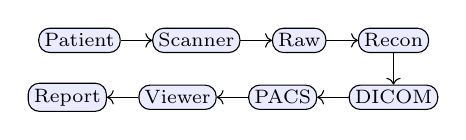
\begin{tikzpicture}[node distance=4mm, every node/.style={font=\scriptsize, draw, rounded corners, inner sep=2pt, fill=blue!8}]
\node (a) {Patient};
\node (b) [right=of a] {Scanner};
\node (c) [right=of b] {Raw};
\node (d) [right=of c] {Recon};
\node (e) [below=of d] {DICOM};
\node (f) [left=of e] {PACS};
\node (g) [left=of f] {Viewer};
\node (h) [left=of g] {Report};
\draw[->] (a)--(b); \draw[->] (b)--(c); \draw[->] (c)--(d);
\draw[->] (d)--(e); \draw[->] (e)--(f); \draw[->] (f)--(g); \draw[->] (g)--(h);
\end{tikzpicture}
\end{center}

\switchcolumn

\subsection*{3.2 Pipeline thu nhận $\to$ tái tạo}
Chuẩn bị bệnh nhân (nhịn ăn, tiêm thuốc cản quang, tư thế) $\to$ quét (tín hiệu thô: \emph{k-space} cho MRI, \emph{sinogram} cho CT, dội RF cho US, list-mode trùng hợp cho PET) $\to$ tái tạo $\to$ hậu xử lý (lọc, MPR, MIP) $\to$ ghi tag DICOM $\to$ máy chủ PACS $\to$ trạm đọc (BS chẩn đoán hình ảnh) $\to$ báo cáo có cấu trúc (HL7/FHIR) $\to$ EMR (hồ sơ bệnh án).

\medskip
\begin{center}
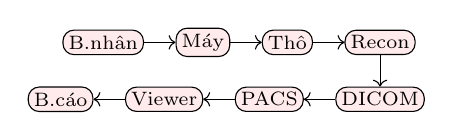
\begin{tikzpicture}[node distance=4mm, every node/.style={font=\scriptsize, draw, rounded corners, inner sep=2pt, fill=red!8}]
\node (a) {B.nhân};
\node (b) [right=of a] {Máy};
\node (c) [right=of b] {Thô};
\node (d) [right=of c] {Recon};
\node (e) [below=of d] {DICOM};
\node (f) [left=of e] {PACS};
\node (g) [left=of f] {Viewer};
\node (h) [left=of g] {B.cáo};
\draw[->] (a)--(b); \draw[->] (b)--(c); \draw[->] (c)--(d);
\draw[->] (d)--(e); \draw[->] (e)--(f); \draw[->] (f)--(g); \draw[->] (g)--(h);
\end{tikzpicture}
\end{center}

\switchcolumn*

% ---------------------------------------------------------------------
% 3.3 Reconstruction methods
% ---------------------------------------------------------------------
\subsection*{3.3 Reconstruction Methods}
\textbf{CT — Filtered Back Projection (FBP).}
Sinogram $p(t,\theta)$ where $t=x\cos\theta+y\sin\theta$.
\begin{enumerate}[leftmargin=*,nosep]
  \item 1D Fourier transform of each projection: $P(\omega,\theta)=\mathcal F_t\{p\}$.
  \item Apply ramp filter $|\omega|$ (often Shepp-Logan / Hann window): $\tilde P=|\omega|P$.
  \item Inverse 1D FT $\to \tilde p(t,\theta)$.
  \item Back-project:
  $$f(x,y)=\int_0^\pi \tilde p(x\cos\theta + y\sin\theta,\theta)\,d\theta$$
\end{enumerate}
\emph{Central Slice Theorem:} 1D FT of projection at angle $\theta$ = central slice of 2D FT of $f$.

\textbf{Iterative CT.}
\begin{itemize}[leftmargin=*,nosep]
  \item ART (Algebraic Reconstruction): Kaczmarz row-action $f^{k+1}=f^k+\lambda \frac{p_i-A_i f^k}{\|A_i\|^2}A_i^T$.
  \item SIRT (Simultaneous), MLEM (max-likelihood expectation maximization, used in PET).
  \item Model-Based Iterative Recon (MBIR): noise model + prior (TV, Markov).
  \item Deep-learning: AUTOMAP, DnCNN-prior, unrolled networks (LEARN, Primal-Dual).
\end{itemize}

\textbf{MRI reconstruction.}
\begin{itemize}[leftmargin=*,nosep]
  \item Fully sampled: $f(x,y)=\mathcal F^{-1}\{S(k_x,k_y)\}$ (2D inverse FFT of k-space).
  \item Parallel imaging: SENSE (image domain unfolding via coil sensitivities), GRAPPA (k-space interpolation).
  \item Compressed sensing: $\min_x \|F_u x-y\|_2^2 + \lambda\|\Psi x\|_1$ (sparsity in wavelet/TV).
  \item DL recon: VarNet, MoDL, AUTOMAP.
\end{itemize}

\textbf{3D Reconstruction from 2D Slices (graphics-relevant).}
\begin{itemize}[leftmargin=*,nosep]
  \item Stack DICOM slices $\to$ regular voxel grid $V(x,y,z)$ with anisotropic spacing.
  \item \textbf{Direct Volume Rendering (DVR):}
    \begin{itemize}[leftmargin=*,nosep]
      \item Ray casting front-to-back; emission-absorption integral
      $$I=\int_0^L C(s)\,\mu(s)\,e^{-\int_0^s\mu(t)dt}\,ds$$
      Discrete compositing: $C_{out}=C_{in}(1-\alpha)+C\alpha$.
      \item Transfer function $\mathrm{TF}:\,\mathrm{intensity}\to(R,G,B,\alpha)$ — tunable for tissue selection.
      \item Variants: splatting (footprint of voxel), 3D texture mapping (GPU slabs), shear-warp (Lacroute \& Levoy), GPU ray-marching.
    \end{itemize}
  \item \textbf{Surface Extraction — Marching Cubes (Lorensen \& Cline 1987):}
    \begin{enumerate}[leftmargin=*,nosep]
      \item For each voxel cube, classify each of 8 corners as inside/outside iso-surface ($\geq T$).
      \item 8-bit index $\to$ one of $2^8=256$ cases; using rotational+reflection symmetry $\to$ 15 base cases.
      \item Lookup table gives edge list; linear interp on each edge:
      $\mathbf p=\mathbf p_a+\frac{T-V_a}{V_b-V_a}(\mathbf p_b-\mathbf p_a)$.
      \item Connect to triangles; estimate normal from $\nabla V$ for shading.
    \end{enumerate}
    \emph{Ambiguity:} same edge index can have two topologies; resolved by \emph{asymptotic decider} (sign of bilinear interp at saddle).
  \item Variants:
    \begin{itemize}[leftmargin=*,nosep]
      \item Marching Tetrahedra (split cube into 5 or 6 tets — no ambiguity, more triangles).
      \item Dual Contouring (Ju et al.) — uses Hermite data on edges, places one vertex per cube via QEF, preserves sharp features.
      \item Cuberille (blocky), Extended/Topological MC.
    \end{itemize}
  \item \textbf{Pipeline:} segment ROI $\to$ MC iso-surface $\to$ smoothing (Taubin $\lambda|\mu$ — keeps volume) $\to$ simplification (QEM — Garland-Heckbert) $\to$ texturing/lighting/render.
\end{itemize}

\textbf{VTK pipeline.}\\
{\scriptsize\ttfamily Reader (vtkDICOMImageReader) $\to$ Filter (vtkImageGaussianSmooth, vtkContourFilter, vtkMarchingCubes) $\to$ Mapper (vtkPolyDataMapper) $\to$ Actor $\to$ Renderer $\to$ RenderWindow+Interactor.}

\switchcolumn

\subsection*{3.3 Phương pháp tái tạo}
\textbf{CT — Filtered Back Projection (FBP).}
Sinogram $p(t,\theta)$ với $t=x\cos\theta+y\sin\theta$.
\begin{enumerate}[leftmargin=*,nosep]
  \item Biến đổi Fourier 1D mỗi hình chiếu: $P(\omega,\theta)=\mathcal F_t\{p\}$.
  \item Áp bộ lọc \emph{ramp} $|\omega|$ (thường kèm cửa sổ Shepp-Logan/Hann): $\tilde P=|\omega|P$.
  \item FT ngược 1D $\to \tilde p(t,\theta)$.
  \item Chiếu ngược:
  $$f(x,y)=\int_0^\pi \tilde p(x\cos\theta + y\sin\theta,\theta)\,d\theta$$
\end{enumerate}
\emph{Định lý lát cắt trung tâm:} FT 1D của hình chiếu góc $\theta$ chính là lát cắt qua tâm của FT 2D của $f$.

\textbf{CT lặp.}
\begin{itemize}[leftmargin=*,nosep]
  \item ART (Đại số): Kaczmarz $f^{k+1}=f^k+\lambda \frac{p_i-A_i f^k}{\|A_i\|^2}A_i^T$.
  \item SIRT (đồng thời), MLEM (cực đại hóa kỳ vọng — dùng trong PET).
  \item MBIR (dựa mô hình): mô hình nhiễu + tiên nghiệm (TV, Markov).
  \item Deep-learning: AUTOMAP, DnCNN-prior, mạng "unrolled" (LEARN, Primal-Dual).
\end{itemize}

\textbf{Tái tạo MRI.}
\begin{itemize}[leftmargin=*,nosep]
  \item Lấy mẫu đầy đủ: $f(x,y)=\mathcal F^{-1}\{S(k_x,k_y)\}$ (FFT ngược 2D từ k-space).
  \item Parallel imaging: SENSE (gỡ rối miền ảnh qua bản đồ độ nhạy cuộn), GRAPPA (nội suy k-space).
  \item Compressed sensing: $\min_x \|F_u x-y\|_2^2 + \lambda\|\Psi x\|_1$ (thưa trên wavelet/TV).
  \item DL recon: VarNet, MoDL, AUTOMAP.
\end{itemize}

\textbf{Tái tạo 3D từ các lát 2D (liên quan đồ họa).}
\begin{itemize}[leftmargin=*,nosep]
  \item Xếp chồng các lát DICOM $\to$ lưới voxel đều $V(x,y,z)$, khoảng cách bất đẳng hướng.
  \item \textbf{Direct Volume Rendering (DVR):}
    \begin{itemize}[leftmargin=*,nosep]
      \item Ray casting front-to-back; tích phân phát xạ-hấp thụ
      $$I=\int_0^L C(s)\,\mu(s)\,e^{-\int_0^s\mu(t)dt}\,ds$$
      Hợp thành rời rạc: $C_{out}=C_{in}(1-\alpha)+C\alpha$.
      \item Transfer function $\mathrm{TF}:\,\mathrm{cường độ}\to(R,G,B,\alpha)$ — chỉnh để chọn loại mô.
      \item Biến thể: splatting (dấu chân voxel), 3D texture (GPU slabs), shear-warp (Lacroute–Levoy), ray-marching trên GPU.
    \end{itemize}
  \item \textbf{Trích bề mặt — Marching Cubes (Lorensen \& Cline 1987):}
    \begin{enumerate}[leftmargin=*,nosep]
      \item Với mỗi khối voxel, phân loại 8 góc bên trong/ngoài bề mặt đẳng trị ($\geq T$).
      \item Chỉ số 8-bit $\to$ một trong $2^8=256$ trường hợp; dùng đối xứng quay+phản xạ $\to$ 15 trường hợp gốc.
      \item Bảng tra tra ra danh sách cạnh; nội suy tuyến tính trên mỗi cạnh:
      $\mathbf p=\mathbf p_a+\frac{T-V_a}{V_b-V_a}(\mathbf p_b-\mathbf p_a)$.
      \item Nối thành tam giác; tính pháp tuyến từ $\nabla V$ để tô bóng.
    \end{enumerate}
    \emph{Mơ hồ:} cùng một chỉ số cạnh có thể có hai topology; xử lý bằng \emph{asymptotic decider} (dấu của nội suy song tuyến tại điểm yên ngựa).
  \item Biến thể:
    \begin{itemize}[leftmargin=*,nosep]
      \item Marching Tetrahedra (chia khối thành 5 hoặc 6 tứ diện — không mơ hồ, nhiều tam giác hơn).
      \item Dual Contouring (Ju et al.) — dùng Hermite trên cạnh, đặt một đỉnh/khối qua QEF, giữ được cạnh sắc.
      \item Cuberille (lập phương), Extended/Topological MC.
    \end{itemize}
  \item \textbf{Quy trình:} phân vùng ROI $\to$ MC iso-surface $\to$ làm mịn (Taubin $\lambda|\mu$ — bảo toàn thể tích) $\to$ giảm tam giác (QEM — Garland-Heckbert) $\to$ gán texture/chiếu sáng/render.
\end{itemize}

\textbf{Pipeline VTK.}\\
{\scriptsize\ttfamily Reader (vtkDICOMImageReader) $\to$ Filter (vtkImageGaussianSmooth, vtkContourFilter, vtkMarchingCubes) $\to$ Mapper (vtkPolyDataMapper) $\to$ Actor $\to$ Renderer $\to$ RenderWindow+Interactor.}

\switchcolumn*

% ---------------------------------------------------------------------
% 3.4 Image processing operations
% ---------------------------------------------------------------------
\subsection*{3.4 Image Processing Operations}
\textbf{Preprocessing.}
\begin{itemize}[leftmargin=*,nosep]
  \item Denoising: Gaussian (LP linear), median (impulse), bilateral (range+space, edge-preserving), non-local means (patch similarity), BM3D, Total Variation, deep denoisers (DnCNN, Noise2Noise).
  \item Contrast: histogram equalization; CLAHE (contrast-limited adaptive HE) per tile + clip.
  \item N4ITK bias-field correction (MRI inhomogeneity, multiplicative low-frequency field).
  \item Intensity normalization: z-score, min-max, percentile clip, white-stripe, Nyul piecewise-linear.
  \item Resampling to isotropic spacing; skull stripping; cropping; padding.
\end{itemize}

\textbf{Registration.}
\begin{itemize}[leftmargin=*,nosep]
  \item Goal: align moving image to fixed image; $T:\mathbb R^3\to\mathbb R^3$.
  \item Rigid (6 DOF — 3 translation + 3 rotation); affine (12 DOF + scale + shear); non-rigid: B-spline FFD (free-form deformation, control grid), Demons (optical flow), diffeomorphic LDDMM (large-deformation), SyN (ANTs).
  \item Similarity metrics: SSD $=\sum(I_f-T(I_m))^2$ (mono-modal), NCC (illumination-invariant), Mutual Information $\mathrm{MI}=H(A)+H(B)-H(A,B)$ (multi-modal MR-CT).
  \item Optimizer: gradient descent, LBFGS, Powell.
  \item DL: VoxelMorph, TransMorph.
\end{itemize}

\textbf{Segmentation.}
\begin{itemize}[leftmargin=*,nosep]
  \item \emph{Thresholding:} Otsu maximizes inter-class variance $\sigma_B^2=w_0w_1(\mu_0-\mu_1)^2$.
  \item \emph{Region growing:} seed + similarity criterion.
  \item \emph{Watershed:} gradient = topographic surface; flood from minima; over-segments $\Rightarrow$ marker-controlled.
  \item \emph{Active contours / Snakes (Kass et al.):} minimize
  $$E=\int(\alpha|C'|^2+\beta|C''|^2+E_{\text{ext}})\,ds$$
  $\alpha$ elasticity, $\beta$ rigidity; $E_{\text{ext}}=-|\nabla(G_\sigma * I)|^2$.
  \item \emph{Level Sets (Osher-Sethian):} embed contour as zero-set of $\phi$; evolve
  $$\frac{\partial\phi}{\partial t}+F|\nabla\phi|=0$$
  Chan-Vese: piecewise-constant Mumford-Shah $\to$ no edge needed.
  \item \emph{Graph cuts:} energy $E=\sum D_p(l_p)+\sum V_{pq}(l_p,l_q)$, min-cut/max-flow $O(V^2E)$ (Boykov-Kolmogorov); GrabCut iterates GMM + graph cut.
  \item \emph{Atlas-based:} register atlas $\to$ propagate labels; multi-atlas + label fusion (majority vote, STAPLE).
  \item \emph{Deep learning:}
    \begin{itemize}[leftmargin=*,nosep]
      \item \textbf{U-Net} (Ronneberger 2015): symmetric encoder-decoder with skip-connections.
      \item \textbf{V-Net} (Milletari 2016): 3D, residual blocks, Dice loss $1-\frac{2|A\cap B|}{|A|+|B|}$.
      \item \textbf{nnU-Net} (Isensee 2021): self-configuring (preprocessing, topology, training); state-of-the-art baseline.
      \item SegResNet, Attention U-Net, TransUNet, Swin-UNet, SAM-Med2D, MedSAM.
    \end{itemize}
\end{itemize}

\textbf{Feature extraction.}
\begin{itemize}[leftmargin=*,nosep]
  \item Gradients: Sobel, Prewitt, Scharr; Canny edge (smooth $\to$ gradient $\to$ NMS $\to$ hysteresis).
  \item Laplacian of Gaussian (LoG), DoG, Hessian (vesselness — Frangi filter).
  \item Texture: GLCM (Haralick: contrast, correlation, energy, homogeneity), LBP, Gabor banks.
  \item \textbf{Radiomics:} shape (volume, sphericity, elongation), first-order intensity (mean, kurtosis), texture (GLCM, GLRLM, GLSZM, NGTDM, GLDM), wavelet/Laplacian filtered features. \textbf{IBSI} standard for reproducibility.
\end{itemize}

\textbf{Classification / Detection.}
\begin{itemize}[leftmargin=*,nosep]
  \item Traditional: SVM (kernel RBF), Random Forest, kNN, AdaBoost — on hand-crafted features.
  \item Deep CNN: LeNet-5, AlexNet, VGG-16/19, GoogLeNet (Inception), ResNet (skip), DenseNet, EfficientNet (compound scaling).
  \item Detection: R-CNN, Fast/Faster R-CNN, YOLO, RetinaNet, DETR.
  \item Vision Transformers: ViT, Swin Transformer, SegFormer.
  \item Foundation models: SAM (Segment Anything), MedSAM, BiomedCLIP, Med-PaLM (text), LLaVA-Med (multi-modal).
\end{itemize}

\switchcolumn

\subsection*{3.4 Các phép xử lý ảnh}
\textbf{Tiền xử lý.}
\begin{itemize}[leftmargin=*,nosep]
  \item Khử nhiễu: Gauss (LP tuyến tính), median (xung), bilateral (giá trị+không gian, giữ cạnh), non-local means (tương đồng patch), BM3D, Total Variation, deep denoiser (DnCNN, Noise2Noise).
  \item Tương phản: cân bằng histogram; CLAHE (cân bằng thích nghi có giới hạn) theo ô + cắt đỉnh.
  \item Hiệu chỉnh từ trường lệch N4ITK (MRI bias field, trường nhân tần số thấp).
  \item Chuẩn hóa cường độ: z-score, min-max, cắt percentile, white-stripe, Nyul phân đoạn tuyến tính.
  \item Resample về spacing đẳng hướng; lột sọ; cắt; pad.
\end{itemize}

\textbf{Đăng ký ảnh (Registration).}
\begin{itemize}[leftmargin=*,nosep]
  \item Mục tiêu: căn ảnh moving với ảnh fixed; $T:\mathbb R^3\to\mathbb R^3$.
  \item Cứng (6 DOF — 3 tịnh tiến + 3 quay); affine (12 DOF + tỷ lệ + cắt); phi cứng: B-spline FFD (biến dạng tự do, lưới điều khiển), Demons (optical flow), diffeomorphic LDDMM (biến dạng lớn), SyN (ANTs).
  \item Hàm tương đồng: SSD $=\sum(I_f-T(I_m))^2$ (đơn modal), NCC (bất biến chiếu sáng), Mutual Information $\mathrm{MI}=H(A)+H(B)-H(A,B)$ (đa modal MR-CT).
  \item Tối ưu hóa: gradient descent, LBFGS, Powell.
  \item DL: VoxelMorph, TransMorph.
\end{itemize}

\textbf{Phân vùng (Segmentation).}
\begin{itemize}[leftmargin=*,nosep]
  \item \emph{Ngưỡng:} Otsu cực đại hóa phương sai liên lớp $\sigma_B^2=w_0w_1(\mu_0-\mu_1)^2$.
  \item \emph{Region growing:} hạt mầm + tiêu chí tương đồng.
  \item \emph{Watershed:} gradient = bề mặt địa hình; tràn từ điểm thấp; dễ over-seg $\Rightarrow$ điều khiển bằng marker.
  \item \emph{Active contour / Snake (Kass):} cực tiểu
  $$E=\int(\alpha|C'|^2+\beta|C''|^2+E_{\text{ext}})\,ds$$
  $\alpha$ co giãn, $\beta$ độ cứng; $E_{\text{ext}}=-|\nabla(G_\sigma * I)|^2$.
  \item \emph{Level Set (Osher-Sethian):} nhúng đường viền là tập-không của $\phi$; tiến hóa
  $$\frac{\partial\phi}{\partial t}+F|\nabla\phi|=0$$
  Chan-Vese: Mumford-Shah từng đoạn-hằng $\to$ không cần cạnh.
  \item \emph{Graph cuts:} năng lượng $E=\sum D_p(l_p)+\sum V_{pq}(l_p,l_q)$, min-cut/max-flow $O(V^2E)$ (Boykov-Kolmogorov); GrabCut lặp GMM + graph cut.
  \item \emph{Dựa atlas:} đăng ký atlas $\to$ truyền nhãn; multi-atlas + hợp nhãn (đa số, STAPLE).
  \item \emph{Học sâu:}
    \begin{itemize}[leftmargin=*,nosep]
      \item \textbf{U-Net} (Ronneberger 2015): encoder-decoder đối xứng, skip-connection.
      \item \textbf{V-Net} (Milletari 2016): 3D, khối residual, Dice loss $1-\frac{2|A\cap B|}{|A|+|B|}$.
      \item \textbf{nnU-Net} (Isensee 2021): tự cấu hình (tiền xử lý, kiến trúc, training); baseline SOTA.
      \item SegResNet, Attention U-Net, TransUNet, Swin-UNet, SAM-Med2D, MedSAM.
    \end{itemize}
\end{itemize}

\textbf{Trích đặc trưng.}
\begin{itemize}[leftmargin=*,nosep]
  \item Gradient: Sobel, Prewitt, Scharr; cạnh Canny (mịn $\to$ gradient $\to$ NMS $\to$ hysteresis).
  \item Laplacian of Gaussian (LoG), DoG, Hessian (mạch máu — Frangi filter).
  \item Texture: GLCM (Haralick: contrast, correlation, energy, homogeneity), LBP, Gabor.
  \item \textbf{Radiomics:} hình dạng (thể tích, độ cầu, độ kéo dài), bậc một (mean, kurtosis), texture (GLCM, GLRLM, GLSZM, NGTDM, GLDM), đặc trưng wavelet/Laplacian. Chuẩn \textbf{IBSI} để tái lập được.
\end{itemize}

\textbf{Phân loại / Phát hiện.}
\begin{itemize}[leftmargin=*,nosep]
  \item Truyền thống: SVM (kernel RBF), Random Forest, kNN, AdaBoost — trên đặc trưng thủ công.
  \item Deep CNN: LeNet-5, AlexNet, VGG-16/19, GoogLeNet (Inception), ResNet (skip), DenseNet, EfficientNet (scale tổng hợp).
  \item Phát hiện: R-CNN, Fast/Faster R-CNN, YOLO, RetinaNet, DETR.
  \item Vision Transformer: ViT, Swin Transformer, SegFormer.
  \item Foundation model: SAM (Segment Anything), MedSAM, BiomedCLIP, Med-PaLM (văn bản), LLaVA-Med (đa modal).
\end{itemize}

\switchcolumn*

% ---------------------------------------------------------------------
% 3.5 Brain tumor detection
% ---------------------------------------------------------------------
\subsection*{3.5 Brain Tumor Detection (BraTS context)}
\textbf{BraTS challenge} (Brain Tumor Segmentation, MICCAI annual since 2012). Provides 4 co-registered MRI modalities per patient:
\begin{itemize}[leftmargin=*,nosep]
  \item \textbf{T1} — anatomy, gray vs white matter.
  \item \textbf{T1ce} (post-Gadolinium) — enhancing tumor highlighted (BBB breakdown).
  \item \textbf{T2} — edema bright.
  \item \textbf{FLAIR} — edema bright, CSF dark (best for whole tumor).
\end{itemize}

\textbf{Tumor sub-regions (labels).}
\begin{itemize}[leftmargin=*,nosep]
  \item \textbf{ET} — Enhancing Tumor (hyper-intense T1ce relative to T1).
  \item \textbf{NCR/NET} — Necrotic / non-enhancing tumor core.
  \item \textbf{ED} — peritumoral Edema.
  \item Hierarchical:
    \begin{itemize}[leftmargin=*,nosep]
      \item \textbf{WT} (Whole Tumor) $=$ ET $\cup$ NCR $\cup$ ED.
      \item \textbf{TC} (Tumor Core) $=$ ET $\cup$ NCR.
      \item \textbf{ET} alone.
    \end{itemize}
\end{itemize}

\textbf{Standard pipeline.}
\begin{enumerate}[leftmargin=*,nosep]
  \item Skull stripping (BET, ROBEX, HD-BET).
  \item Co-registration of 4 modalities (rigid to T1 atlas, e.g., SRI24).
  \item Bias field correction (N4ITK).
  \item Resample to 1\,mm$^3$ isotropic.
  \item Intensity normalization (z-score per modality, brain mask).
  \item Patch / full-volume training of 3D U-Net / nnU-Net.
  \item Inference + post-processing: connected components, fill holes, conditional random field (CRF), morphology, ensemble (TTA, k-fold).
\end{enumerate}

\textbf{Evaluation metrics.}
\begin{itemize}[leftmargin=*,nosep]
  \item \textbf{Dice} $=\dfrac{2|A\cap B|}{|A|+|B|}\in[0,1]$, harmonic mean of precision/recall.
  \item \textbf{Jaccard / IoU} $=\dfrac{|A\cap B|}{|A\cup B|}=\dfrac{D}{2-D}$.
  \item \textbf{Hausdorff95} $=$ 95-th percentile of $\{d(a,B)\}\cup\{d(b,A)\}$ — robust to outliers.
  \item \textbf{ASSD} $=\dfrac{1}{|S_A|+|S_B|}\!\!\left(\!\sum_{a\in S_A}\!d(a,S_B)\!+\!\!\sum_{b\in S_B}\!d(b,S_A)\!\right)$.
  \item Sensitivity $=\mathrm{TP/(TP+FN)}$, Specificity $=\mathrm{TN/(TN+FP)}$, Precision, Recall, F1.
  \item Volumetric similarity, Cohen's $\kappa$, AUC for classification heads.
\end{itemize}

\switchcolumn

\subsection*{3.5 Phát hiện u não (BraTS)}
\textbf{Thử thách BraTS} (MICCAI hàng năm từ 2012). Mỗi bệnh nhân có 4 modality MRI đã đăng ký:
\begin{itemize}[leftmargin=*,nosep]
  \item \textbf{T1} — giải phẫu, chất xám/trắng.
  \item \textbf{T1ce} (sau Gadolinium) — vùng u tăng quang (hàng rào máu não bị phá).
  \item \textbf{T2} — phù não sáng.
  \item \textbf{FLAIR} — phù sáng, dịch não tủy tối (tốt nhất cho whole tumor).
\end{itemize}

\textbf{Vùng u con (nhãn).}
\begin{itemize}[leftmargin=*,nosep]
  \item \textbf{ET} — Enhancing Tumor (tăng quang T1ce so với T1).
  \item \textbf{NCR/NET} — hoại tử / không tăng quang.
  \item \textbf{ED} — phù quanh u.
  \item Phân cấp:
    \begin{itemize}[leftmargin=*,nosep]
      \item \textbf{WT} (Toàn bộ u) $=$ ET $\cup$ NCR $\cup$ ED.
      \item \textbf{TC} (Lõi u) $=$ ET $\cup$ NCR.
      \item \textbf{ET} riêng.
    \end{itemize}
\end{itemize}

\textbf{Pipeline chuẩn.}
\begin{enumerate}[leftmargin=*,nosep]
  \item Lột sọ (BET, ROBEX, HD-BET).
  \item Đăng ký đồng vị 4 modality (cứng về atlas T1, vd SRI24).
  \item Hiệu chỉnh bias field (N4ITK).
  \item Resample về 1\,mm$^3$ đẳng hướng.
  \item Chuẩn hóa cường độ (z-score mỗi modality, mask não).
  \item Train 3D U-Net / nnU-Net theo patch hoặc full-volume.
  \item Suy luận + hậu xử lý: thành phần liên thông, lấp lỗ, CRF, hình thái, ensemble (TTA, k-fold).
\end{enumerate}

\textbf{Độ đo đánh giá.}
\begin{itemize}[leftmargin=*,nosep]
  \item \textbf{Dice} $=\dfrac{2|A\cap B|}{|A|+|B|}\in[0,1]$, trung bình điều hòa precision/recall.
  \item \textbf{Jaccard / IoU} $=\dfrac{|A\cap B|}{|A\cup B|}=\dfrac{D}{2-D}$.
  \item \textbf{Hausdorff95} $=$ percentile thứ 95 của $\{d(a,B)\}\cup\{d(b,A)\}$ — kháng outlier.
  \item \textbf{ASSD} $=\dfrac{1}{|S_A|+|S_B|}\!\!\left(\!\sum_{a\in S_A}\!d(a,S_B)\!+\!\!\sum_{b\in S_B}\!d(b,S_A)\!\right)$.
  \item Sensitivity $=\mathrm{TP/(TP+FN)}$, Specificity $=\mathrm{TN/(TN+FP)}$, Precision, Recall, F1.
  \item Tương đồng thể tích, Cohen's $\kappa$, AUC cho head phân loại.
\end{itemize}

\switchcolumn*

% ---------------------------------------------------------------------
% 3.6 Paper 1 summary (GAN brain tumor)
% ---------------------------------------------------------------------
\subsection*{3.6 Paper 1 — GAN Brain Tumor Segmentation}
\textbf{Title:} \emph{A Research for Segmentation of Brain Tumors Based on GAN Model.} Multi-scale 3D-GAN evaluated on BraTS 2021.

\textbf{Architecture.}
\begin{itemize}[leftmargin=*,nosep]
  \item \textbf{Generator $G$:} 3D Residual U-Net (encoder-decoder with residual blocks, skip connections, 3D convs).
  \item \textbf{Bridge module:} sits between $G$ and Discriminator; aggregates multi-scale features from several $G$ decoder stages, fuses them, and feeds into $D$ so that $D$ sees both high-level context and low-level boundary details simultaneously.
  \item \textbf{Discriminator $D$:} judges (input MRI $\oplus$ predicted seg) vs (input $\oplus$ ground truth).
\end{itemize}

\textbf{Three contributions.}
\begin{enumerate}[leftmargin=*,nosep]
  \item Bridge module — fuses multi-scale features into $D$.
  \item \textbf{Algorithm 1} — dynamically adjusts the number of $D$ training epochs using the linear-regression \emph{slope} of the adversarial loss; if loss is decreasing too fast, train $D$ more (or less) to balance $G$-vs-$D$.
  \item Combined loss: $\mathcal L=\mathcal L_{\text{Dice}}+\lambda \mathcal L_{\text{MSE-adv}}$.
\end{enumerate}

\textbf{Results (Dice, BraTS 2021 validation split).}
\begin{itemize}[leftmargin=*,nosep]
  \item ET = 82.3\%, WT = 88.6\%, TC = 83.1\% — beats U-Net, V-Net, VoxelGAN, Vox2Vox.
  \item Also reports Jaccard, Hausdorff95, ASSD vs same baselines.
\end{itemize}

\textbf{Strengths.}
\begin{itemize}[leftmargin=*,nosep]
  \item Bridge well-motivated: gives $D$ both context + boundary detail.
  \item Algorithm 1 is novel and pragmatic — addresses classic GAN G-D imbalance.
  \item 4 metrics (Dice, Jaccard, HD95, ASSD) and 4 baselines (CNN + GAN families).
\end{itemize}

\textbf{Weaknesses.}
\begin{itemize}[leftmargin=*,nosep]
  \item Only validation split from training — no cross-validation, no submission to BraTS server $\Rightarrow$ hard to compare with literature.
  \item No ablation isolating Bridge vs Algorithm 1 — individual contribution unknown.
  \item \emph{Paradox:} on ET, GAN gives higher Dice than ResUnet-no-GAN but \emph{worse} HD95 (9.6\,mm vs 6.4\,mm) and ASSD (3.37 vs 2.35) $\Rightarrow$ GAN improved overlap but \emph{degraded boundary}.
  \item Hyperparams of Algorithm 1 ($k$, $l$, threshold $\beta$) untuned; no theoretical justification for linear regression on adversarial loss.
  \item No parameter count, training/inference time, no significance tests, no code release.
  \item Bridge module deserves its own dedicated figure (currently merged in Fig.\,1).
\end{itemize}

\textbf{Suggested improvements.}
\begin{itemize}[leftmargin=*,nosep]
  \item Submit to BraTS online server, or 5-fold CV with mean$\pm$std.
  \item Ablations: Baseline / +Bridge / +Algo1 / +both.
  \item Analyze ET HD95/ASSD paradox (boundary smoothing artifacts of MSE-adv?).
  \item Sensitivity analysis on $k,l,\beta$.
  \item Release source code; report params/FLOPs/runtime; statistical significance (paired Wilcoxon).
\end{itemize}

\switchcolumn

\subsection*{3.6 Paper 1 — GAN phân vùng u não}
\textbf{Tiêu đề:} \emph{A Research for Segmentation of Brain Tumors Based on GAN Model.} Multi-scale 3D-GAN, đánh giá trên BraTS 2021.

\textbf{Kiến trúc.}
\begin{itemize}[leftmargin=*,nosep]
  \item \textbf{Generator $G$:} 3D Residual U-Net (encoder-decoder với khối residual, skip connection, conv 3D).
  \item \textbf{Bridge module:} nằm giữa $G$ và Discriminator; tổng hợp đặc trưng đa tỷ lệ từ vài tầng decoder của $G$, hợp nhất rồi đưa vào $D$ để $D$ nhìn được cả ngữ cảnh cấp cao lẫn chi tiết biên cấp thấp.
  \item \textbf{Discriminator $D$:} phân biệt (MRI $\oplus$ seg dự đoán) vs (MRI $\oplus$ ground truth).
\end{itemize}

\textbf{Ba đóng góp.}
\begin{enumerate}[leftmargin=*,nosep]
  \item Bridge module — hợp đặc trưng đa tỷ lệ vào $D$.
  \item \textbf{Algorithm 1} — điều chỉnh động số epoch huấn luyện $D$ theo \emph{độ dốc} hồi quy tuyến tính của adversarial loss; nếu loss giảm quá nhanh thì train $D$ thêm (hoặc bớt) để cân bằng $G$-$D$.
  \item Hàm loss kết hợp: $\mathcal L=\mathcal L_{\text{Dice}}+\lambda \mathcal L_{\text{MSE-adv}}$.
\end{enumerate}

\textbf{Kết quả (Dice, validation split BraTS 2021).}
\begin{itemize}[leftmargin=*,nosep]
  \item ET = 82.3\%, WT = 88.6\%, TC = 83.1\% — vượt U-Net, V-Net, VoxelGAN, Vox2Vox.
  \item Báo cáo thêm Jaccard, Hausdorff95, ASSD so cùng baselines.
\end{itemize}

\textbf{Điểm mạnh.}
\begin{itemize}[leftmargin=*,nosep]
  \item Bridge có động cơ rõ: cho $D$ cả ngữ cảnh + chi tiết biên.
  \item Algorithm 1 mới và thực dụng — xử lý mất cân bằng kinh điển G-D trong GAN.
  \item 4 độ đo (Dice, Jaccard, HD95, ASSD) và 4 baseline (CNN + GAN).
\end{itemize}

\textbf{Điểm yếu.}
\begin{itemize}[leftmargin=*,nosep]
  \item Chỉ chia validation từ training — không cross-validation, không nộp BraTS server $\Rightarrow$ khó so với cộng đồng.
  \item Thiếu ablation tách bạch Bridge vs Algorithm 1 — không biết phần nào đóng góp bao nhiêu.
  \item \emph{Nghịch lý:} với ET, GAN có Dice cao hơn ResUnet không-GAN nhưng HD95 (9.6\,mm vs 6.4\,mm) và ASSD (3.37 vs 2.35) lại \emph{tệ hơn} $\Rightarrow$ GAN cải thiện overlap thể tích nhưng \emph{làm xấu biên}.
  \item Siêu tham số Algorithm 1 ($k$, $l$, ngưỡng $\beta$) không khảo sát; không có lý thuyết nào biện minh cho việc hồi quy tuyến tính trên loss.
  \item Không có số tham số, thời gian train/infer, không có kiểm định ý nghĩa thống kê, không công khai code.
  \item Module Bridge đáng có hình riêng (đang gộp vào Fig.\,1).
\end{itemize}

\textbf{Đề xuất cải tiến.}
\begin{itemize}[leftmargin=*,nosep]
  \item Nộp BraTS online server, hoặc 5-fold CV với mean$\pm$std.
  \item Ablation: Baseline / +Bridge / +Algo1 / +cả hai.
  \item Phân tích nghịch lý HD95/ASSD ở ET (nghi do MSE-adv làm trơn biên?).
  \item Khảo sát độ nhạy $k,l,\beta$.
  \item Công khai mã nguồn; báo cáo params/FLOPs/runtime; kiểm định ý nghĩa (paired Wilcoxon).
\end{itemize}

\switchcolumn*

% ---------------------------------------------------------------------
% 3.7 Paper 2 summary (ANN -> DCNN)
% ---------------------------------------------------------------------
\subsection*{3.7 Paper 2 — ANN $\to$ DCNN Paradigm Shift Review}
\textbf{Title:} \emph{Paradigm shift from Artificial Neural Networks (ANNs) to deep Convolutional Neural Networks (DCNNs) in the field of medical image processing.} 2024 review.

\textbf{Thesis.} Past pipeline: hand-crafted feature extraction (SIFT, GLCM, Hu moments) $\to$ shallow ANN classifier. Modern pipeline: end-to-end DCNN learns features directly from raw images.

\textbf{Strengths.}
\begin{itemize}[leftmargin=*,nosep]
  \item Concrete numerical convolution example with a Sobel kernel applied to a hand X-ray $\Rightarrow$ very accessible for newcomers.
  \item Two summary tables: ANN-based vs DCNN-based studies — \emph{the "feature extraction" column literally vanishes} in DCNN row.
  \item Honest about DCNN limitations: data-hungry, prone to overfitting, black-box.
\end{itemize}

\textbf{Weaknesses.}
\begin{itemize}[leftmargin=*,nosep]
  \item No mention of \textbf{Vision Transformers}, \textbf{SAM}, or medical foundation models (Med-PaLM, LLaVA-Med) — yet the paper claims a "paradigm shift" in 2024. The actual ongoing shift (DCNN $\to$ Transformer/Foundation) is ignored. ANN $\to$ DCNN was already widely accepted by 2017.
  \item Focuses on \textbf{classification}; ignores \textbf{segmentation} (U-Net, nnU-Net) and standard datasets (\textbf{BraTS}, LIDC, CheXpert).
  \item English-language context only; no \textbf{low-resource language} coverage. Critical for Vietnamese CDSS — labeled corpora missing, mixed VN-EN-Latin terminology, no local medical knowledge graph.
  \item No \textbf{XAI} (Grad-CAM, conformal prediction, Dempster-Shafer) and no \textbf{uncertainty quantification} — yet the EU AI Act classifies CDSS as \emph{high-risk}, so explainability is mandatory.
  \item No PRISMA / inclusion-exclusion criteria for a review paper; no positioning vs Litjens 2017 / Esteva 2019 (already authoritative surveys).
  \item Long, rambling history (1980s--90s) padding; the actually-important CNN mechanism section is too short. AI/ML/DL definition boxes are too basic for a Q1 journal.
\end{itemize}

\textbf{Takeaway.} Useful intro for newcomers, but for proper publication needs: (i) Transformers + foundation models, (ii) segmentation track + standard datasets, (iii) low-resource language section, (iv) XAI + uncertainty for CDSS, (v) PRISMA methodology and survey-positioning.

\switchcolumn

\subsection*{3.7 Paper 2 — Tổng quan chuyển dịch ANN $\to$ DCNN}
\textbf{Tiêu đề:} \emph{Paradigm shift from Artificial Neural Networks (ANNs) to deep Convolutional Neural Networks (DCNNs) in the field of medical image processing.} Bài tổng quan 2024.

\textbf{Luận điểm.} Quy trình cũ: trích đặc trưng thủ công (SIFT, GLCM, mô-men Hu) $\to$ ANN nông để phân loại. Quy trình hiện đại: DCNN end-to-end học đặc trưng trực tiếp từ ảnh thô.

\textbf{Điểm mạnh.}
\begin{itemize}[leftmargin=*,nosep]
  \item Ví dụ tích chập số cụ thể với kernel Sobel áp lên ảnh X-quang bàn tay $\Rightarrow$ rất dễ hiểu cho người mới.
  \item Hai bảng tổng kết: nghiên cứu dùng ANN vs nghiên cứu dùng DCNN — \emph{cột "feature extraction" biến mất hoàn toàn} ở dòng DCNN.
  \item Trung thực về hạn chế của DCNN: cần nhiều dữ liệu, dễ overfit, hộp đen.
\end{itemize}

\textbf{Điểm yếu.}
\begin{itemize}[leftmargin=*,nosep]
  \item Không nhắc đến \textbf{Vision Transformer}, \textbf{SAM}, hay các foundation model y tế (Med-PaLM, LLaVA-Med) — mà bài lại tuyên bố "paradigm shift" năm 2024. Cuộc chuyển dịch đang xảy ra (DCNN $\to$ Transformer/Foundation) bị bỏ qua. ANN $\to$ DCNN đã được công nhận từ 2017.
  \item Chỉ tập trung \textbf{phân loại}; bỏ qua \textbf{phân vùng} (U-Net, nnU-Net) và các bộ dữ liệu chuẩn (\textbf{BraTS}, LIDC, CheXpert).
  \item Bối cảnh chỉ tiếng Anh; không đề cập \textbf{ngôn ngữ low-resource}. Rất quan trọng với CDSS tiếng Việt — thiếu corpus có nhãn, thuật ngữ trộn VN-EN-Latin, chưa có knowledge graph y tế Việt.
  \item Không bàn \textbf{XAI} (Grad-CAM, conformal prediction, Dempster-Shafer) lẫn \textbf{đo bất định} — nhưng EU AI Act xếp CDSS vào \emph{high-risk} nên giải thích được là bắt buộc.
  \item Bài tổng quan mà không có PRISMA / tiêu chí lựa chọn-loại trừ; không định vị so với Litjens 2017 / Esteva 2019 (đã là survey kinh điển).
  \item Phần lịch sử (1980s--90s) dài lan man; phần cơ chế CNN — phần quan trọng — lại quá ngắn. Hộp định nghĩa AI/ML/DL quá cơ bản cho một tạp chí Q1.
\end{itemize}

\textbf{Tóm lại.} Hữu ích như bài đọc nhập môn, nhưng để xuất bản đàng hoàng cần: (i) Transformer + foundation models, (ii) nhánh segmentation + dataset chuẩn, (iii) phần ngôn ngữ low-resource, (iv) XAI + uncertainty cho CDSS, (v) phương pháp PRISMA và định vị so với survey trước.

\switchcolumn*

% ---------------------------------------------------------------------
% 3.8 Diagnosis-support applications
% ---------------------------------------------------------------------
\subsection*{3.8 Diagnosis-Support Applications}
\textbf{Use cases.}
\begin{itemize}[leftmargin=*,nosep]
  \item Triage / worklist prioritization (e.g., critical findings in head CT).
  \item Second-reader / double-reading (mammography).
  \item Population screening (chest X-ray TB, retinal DR, breast cancer).
  \item Surgical planning (3D mesh from CT/MRI for tumor resection).
  \item Image-guided intervention (real-time fusion US+MRI for biopsy/ablation).
  \item Quantification: lesion volume, perfusion, ejection fraction.
  \item Treatment response monitoring (RECIST, longitudinal radiomics).
\end{itemize}

\textbf{End-to-end CDSS pipeline.}
DICOM input $\to$ preprocessing (denoise, normalize, register) $\to$ segmentation (U-Net family) $\to$ classification / detection (CNN/ViT) $\to$ uncertainty quantification (MC-Dropout, deep ensembles, conformal prediction) $\to$ explanation (Grad-CAM, Integrated Gradients, attention maps, SHAP) $\to$ structured report (HL7 FHIR DiagnosticReport) $\to$ clinician review.

\textbf{Regulatory.}
\begin{itemize}[leftmargin=*,nosep]
  \item \textbf{FDA 510(k)} / De Novo / PMA in US; AI/ML SaMD action plan; predetermined change control.
  \item \textbf{CE marking}, \textbf{MDR} (EU 2017/745).
  \item \textbf{EU AI Act} — CDSS is high-risk: requires risk-management, data governance, technical docs, transparency, human oversight, accuracy/robustness/cybersecurity logs.
  \item Privacy: HIPAA (US), GDPR (EU), Vietnam Decree 13/2023/ND-CP on personal data.
\end{itemize}

\textbf{Vietnamese context.}
\begin{itemize}[leftmargin=*,nosep]
  \item Lacking large-scale Vietnamese-labeled medical corpora (radiology reports, clinical notes).
  \item Mixed VN-EN-Latin terminology (e.g., "viêm phổi / pneumonia / bronchopneumonia").
  \item Missing local medical knowledge graph / SNOMED-CT Vietnamese mapping.
  \item Hospital PACS/HIS heterogeneous; limited GPU; class imbalance for rare endemic diseases.
\end{itemize}

\switchcolumn

\subsection*{3.8 Ứng dụng hỗ trợ chẩn đoán}
\textbf{Trường hợp sử dụng.}
\begin{itemize}[leftmargin=*,nosep]
  \item Phân loại ưu tiên / triage (vd phát hiện CT sọ não nguy kịch).
  \item Người đọc thứ hai / đọc kép (nhũ ảnh).
  \item Tầm soát quần thể (X-quang phổi lao, võng mạc tiểu đường, ung thư vú).
  \item Lập kế hoạch phẫu thuật (mesh 3D từ CT/MRI để cắt u).
  \item Can thiệp dưới hình ảnh (hợp nhất US+MRI thời gian thực để sinh thiết/đốt).
  \item Định lượng: thể tích tổn thương, tưới máu, phân suất tống máu.
  \item Theo dõi đáp ứng điều trị (RECIST, radiomics dọc).
\end{itemize}

\textbf{Pipeline CDSS đầu cuối.}
DICOM đầu vào $\to$ tiền xử lý (khử nhiễu, chuẩn hóa, đăng ký) $\to$ phân vùng (họ U-Net) $\to$ phân loại / phát hiện (CNN/ViT) $\to$ đo bất định (MC-Dropout, deep ensembles, conformal prediction) $\to$ giải thích (Grad-CAM, Integrated Gradients, bản đồ chú ý, SHAP) $\to$ báo cáo có cấu trúc (HL7 FHIR DiagnosticReport) $\to$ bác sĩ duyệt.

\textbf{Pháp lý.}
\begin{itemize}[leftmargin=*,nosep]
  \item \textbf{FDA 510(k)} / De Novo / PMA tại Mỹ; kế hoạch SaMD AI/ML; kiểm soát thay đổi đã định trước.
  \item \textbf{CE marking}, \textbf{MDR} (EU 2017/745).
  \item \textbf{EU AI Act} — CDSS thuộc nhóm rủi ro cao: yêu cầu quản lý rủi ro, quản trị dữ liệu, tài liệu kỹ thuật, minh bạch, giám sát của người, log độ chính xác/độ bền/an ninh mạng.
  \item Bảo mật: HIPAA (Mỹ), GDPR (EU), Nghị định 13/2023/NĐ-CP về dữ liệu cá nhân ở Việt Nam.
\end{itemize}

\textbf{Bối cảnh Việt Nam.}
\begin{itemize}[leftmargin=*,nosep]
  \item Thiếu corpus y tế tiếng Việt có nhãn quy mô lớn (báo cáo chẩn đoán hình ảnh, ghi chú lâm sàng).
  \item Thuật ngữ trộn VN-EN-Latin (vd "viêm phổi / pneumonia / bronchopneumonia").
  \item Chưa có knowledge graph y tế tiếng Việt / ánh xạ SNOMED-CT.
  \item PACS/HIS bệnh viện không đồng nhất; GPU hạn chế; mất cân bằng lớp với bệnh đặc hữu hiếm.
\end{itemize}

\switchcolumn*

% ---------------------------------------------------------------------
% 3.9 Quick reference summary table
% ---------------------------------------------------------------------
\subsection*{3.9 Quick Reference Summary}
\scriptsize
\setlength{\tabcolsep}{2pt}
\begin{tabular}{@{}p{1.1cm}p{2.2cm}p{2.5cm}p{2.5cm}@{}}
\toprule
Mod. & Best for & Reconstruction & Mesh extraction \\
\midrule
MRI & soft tissue, brain, MS & 2D iFFT k-space; SENSE/GRAPPA; CS & MC on T1/FLAIR after seg. \\
CT & bone, lung, trauma & FBP (ramp); iter MBIR; DL recon & MC on HU threshold (bone $>$300) \\
US 3D & OB, cardiac, vascular & beamforming; freehand 3D & MC on B-mode envelope (noisy) \\
PET & oncology, brain metab. & MLEM, OSEM, TOF & threshold SUV $\to$ MC, smooth \\
X-ray & chest, mammo & none (2D projection) & N/A (unless tomosynth.) \\
SPECT & cardiac, bone, thyroid & FBP / OSEM & rare \\
OCT & retina, anterior segment & Fourier-domain iFFT & MC on layer prob. map \\
\bottomrule
\end{tabular}
\normalsize

\medskip
\textbf{Key formulas to remember.}
\begin{itemize}[leftmargin=*,nosep]
  \item HU: $\mathrm{HU}=1000(\mu-\mu_w)/\mu_w$.
  \item Larmor: $\omega_0=\gamma B_0$ ($\gamma_{^1\!H}/2\pi=42.58$ MHz/T).
  \item FBP: $f(x,y)=\!\int_0^\pi\!\tilde p(x\cos\theta+y\sin\theta,\theta)d\theta$.
  \item MC edge interp: $\mathbf p=\mathbf p_a+\frac{T-V_a}{V_b-V_a}(\mathbf p_b-\mathbf p_a)$.
  \item DVR composite: $C_{out}=C_{in}(1-\alpha)+C\alpha$.
  \item Dice: $D=2|A\cap B|/(|A|+|B|)$; IoU $=D/(2-D)$.
  \item Otsu: $\arg\max_T w_0w_1(\mu_0-\mu_1)^2$.
  \item Snake energy: $E=\!\int(\alpha|C'|^2+\beta|C''|^2+E_{\text{ext}})ds$.
  \item Level set: $\partial\phi/\partial t+F|\nabla\phi|=0$.
  \item MI: $\mathrm{MI}(A,B)=H(A)+H(B)-H(A,B)$.
\end{itemize}

\switchcolumn

\subsection*{3.9 Bảng tổng kết tham khảo nhanh}
\scriptsize
\begin{tabular}{@{}llll@{}}
\toprule
P.thức & Tốt cho & Tái tạo & Trích mesh \\
\midrule
MRI & mô mềm, não, MS & iFFT 2D k-space; SENSE/GRAPPA; CS & MC trên T1/FLAIR sau seg \\
CT & xương, phổi, ch.thương & FBP (ramp); MBIR lặp; DL recon & MC ngưỡng HU (xương $>$300) \\
US 3D & sản, tim, mạch & beamforming; 3D tự do & MC trên envelope B-mode, nhiễu \\
PET & ung thư, ch.hóa não & MLEM, OSEM, TOF & ngưỡng SUV $\to$ MC, làm mịn \\
X-q & ngực, vú & không (chiếu 2D) & N/A (trừ tomosynthesis) \\
SPECT & tim, xương, giáp & FBP / OSEM & hiếm \\
OCT & võng mạc, đoạn trước & FT ngược miền Fourier & MC trên bản đồ xác suất lớp \\
\bottomrule
\end{tabular}
\normalsize

\medskip
\textbf{Công thức cần nhớ.}
\begin{itemize}[leftmargin=*,nosep]
  \item HU: $\mathrm{HU}=1000(\mu-\mu_w)/\mu_w$.
  \item Larmor: $\omega_0=\gamma B_0$ ($\gamma_{^1\!H}/2\pi=42.58$ MHz/T).
  \item FBP: $f(x,y)=\!\int_0^\pi\!\tilde p(x\cos\theta+y\sin\theta,\theta)d\theta$.
  \item Nội suy cạnh MC: $\mathbf p=\mathbf p_a+\frac{T-V_a}{V_b-V_a}(\mathbf p_b-\mathbf p_a)$.
  \item Hợp DVR: $C_{out}=C_{in}(1-\alpha)+C\alpha$.
  \item Dice: $D=2|A\cap B|/(|A|+|B|)$; IoU $=D/(2-D)$.
  \item Otsu: $\arg\max_T w_0w_1(\mu_0-\mu_1)^2$.
  \item Năng lượng Snake: $E=\!\int(\alpha|C'|^2+\beta|C''|^2+E_{\text{ext}})ds$.
  \item Level set: $\partial\phi/\partial t+F|\nabla\phi|=0$.
  \item MI: $\mathrm{MI}(A,B)=H(A)+H(B)-H(A,B)$.
\end{itemize}

\end{paracol}


\vfill\hrule\vspace{4pt}

% =====================================================================
% 04_bezier.tex  --  Bezier Curves, Bezier Surfaces, De Casteljau
% Bilingual EN | VI cheatsheet section for IT516 Advanced Computer Graphics
% =====================================================================

\section*{4.\ Bezier Curves, Bezier Surfaces, De Casteljau \;|\; \textit{Đường cong, Mặt Bezier, Thuật toán De Casteljau}}

\begin{paracol}{2}

% ---------------------------------------------------------------------
% 4.1  DEFINITION & BERNSTEIN FORM
% ---------------------------------------------------------------------
\subsection*{4.1 Bezier Curve --- Bernstein Form}

A \textbf{Bezier curve} of degree $n$ with $n{+}1$ control points $P_0,\dots,P_n$ is the parametric curve
\[
B(t)=\sum_{i=0}^{n}\binom{n}{i}(1-t)^{\,n-i}t^{\,i}P_i,\quad t\in[0,1].
\]
The polynomials
\[
B_i^{\,n}(t)=\binom{n}{i}(1-t)^{\,n-i}t^{\,i},\quad i=0,\dots,n
\]
are called \textbf{Bernstein basis polynomials}.

\textbf{Key properties.}
\begin{itemize}[leftmargin=*,nosep]
  \item \emph{Endpoint interpolation:} $B(0)=P_0,\ B(1)=P_n$.
  \item \emph{Partition of unity:} $\sum_{i=0}^{n}B_i^{\,n}(t)=1$ for all $t$ $\Rightarrow$ \emph{affine invariance}.
  \item \emph{Convex hull:} $B(t)\in\operatorname{conv}\{P_0,\dots,P_n\}$ since $B_i^{\,n}(t)\ge 0$.
  \item \emph{Variation diminishing:} the curve crosses any line/plane no more times than its control polygon does $\Rightarrow$ no extra wiggles.
  \item \emph{Symmetry:} $B(t)$ with control points reversed equals $B(1{-}t)$, i.e.\ $B_i^{\,n}(t)=B_{n-i}^{\,n}(1-t)$.
  \item \emph{Endpoint tangents:}
        $B'(0)=n(P_1-P_0),\ B'(1)=n(P_n-P_{n-1})$.
  \item \emph{Pseudo-local control:} moving $P_i$ shifts $B(t)$ proportionally to $B_i^{\,n}(t)$ (max at $t=i/n$).
  \item \emph{Degree:} a Bezier curve with $n{+}1$ points is a polynomial of degree $\le n$.
\end{itemize}

\switchcolumn

\subsection*{4.1 Đường cong Bezier --- Dạng Bernstein}

\textbf{Đường cong Bezier} bậc $n$ với $n{+}1$ control point $P_0,\dots,P_n$ là đường cong tham số
\[
B(t)=\sum_{i=0}^{n}\binom{n}{i}(1-t)^{\,n-i}t^{\,i}P_i,\quad t\in[0,1].
\]
Các đa thức $B_i^{\,n}(t)=\binom{n}{i}(1-t)^{\,n-i}t^{\,i}$ gọi là \textbf{đa thức cơ sở Bernstein}.

\textbf{Tính chất quan trọng.}
\begin{itemize}[leftmargin=*,nosep]
  \item \emph{Nội suy đầu mút:} $B(0)=P_0,\ B(1)=P_n$.
  \item \emph{Tổng bằng 1:} $\sum B_i^{\,n}(t)=1$ $\Rightarrow$ \emph{bất biến affine} (xoay/tịnh tiến control point thì curve cũng biến đổi tương ứng).
  \item \emph{Bao lồi:} đường cong luôn nằm trong bao lồi của các control point.
  \item \emph{Giảm dao động (variation diminishing):} đường cong cắt một đường thẳng không nhiều hơn số lần control polygon cắt đường đó.
  \item \emph{Đối xứng:} đảo thứ tự control point thì $B(t)$ trở thành $B(1{-}t)$.
  \item \emph{Tiếp tuyến tại đầu mút:}
        $B'(0)=n(P_1-P_0)$, $B'(1)=n(P_n-P_{n-1})$.
  \item \emph{Điều khiển gần địa phương:} khi dời $P_i$, curve dịch chuyển nhiều nhất tại $t=i/n$.
  \item \emph{Bậc:} curve là đa thức bậc $\le n$.
\end{itemize}

\switchcolumn*

% ---------------------------------------------------------------------
% 4.2  SPECIFIC CASES
% ---------------------------------------------------------------------
\subsection*{4.2 Specific Low Degrees}

\textbf{Linear} ($n=1$, $P_0,P_1$):
\[
B(t)=(1-t)P_0+tP_1.
\]
\textbf{Quadratic} ($n=2$, $P_0,P_1,P_2$):
\[
B(t)=(1-t)^{2}P_0+2(1-t)tP_1+t^{2}P_2.
\]
\textbf{Cubic} ($n=3$, $P_0,P_1,P_2,P_3$) -- the most-used in graphics:
\[
B(t)=(1-t)^{3}P_0+3(1-t)^{2}tP_1+3(1-t)t^{2}P_2+t^{3}P_3.
\]
\textbf{Quartic} ($n=4$):
\[
B(t)=\sum_{i=0}^{4}\binom{4}{i}(1-t)^{4-i}t^{\,i}P_i.
\]

\textbf{Pascal's triangle} (binomial coefficients):
\begin{center}\small
\begin{tabular}{c|ccccccc}
$n$ & & & & coefficients & & & \\\midrule
0 & & & & 1 & & & \\
1 & & & 1 & & 1 & & \\
2 & & & 1 & 2 & 1 & & \\
3 & & 1 & 3 & 3 & 1 & & \\
4 & 1 & 4 & 6 & 4 & 1 & & \\
5 & 1 & 5 & 10 & 10 & 5 & 1 & \\
\end{tabular}
\end{center}

\switchcolumn

\subsection*{4.2 Một số bậc thường gặp}

\textbf{Tuyến tính} ($n=1$): $B(t)=(1-t)P_0+tP_1$ -- chính là phép nội suy tuyến tính giữa hai điểm.

\textbf{Bậc hai} ($n=2$):
$B(t)=(1-t)^{2}P_0+2(1-t)tP_1+t^{2}P_2$.

\textbf{Bậc ba} ($n=3$) -- thông dụng nhất trong đồ hoạ và font chữ:
$B(t)=(1-t)^{3}P_0+3(1-t)^{2}tP_1+3(1-t)t^{2}P_2+t^{3}P_3$.

\textbf{Bậc bốn} ($n=4$): tương tự, hệ số $\binom{4}{i}=1,4,6,4,1$.

\textbf{Tam giác Pascal} dùng để tra hệ số nhị thức $\binom{n}{i}$:
\begin{center}\small
\begin{tabular}{c|ccccccc}
$n$ & & & & hệ số & & & \\\midrule
0 & & & & 1 & & & \\
1 & & & 1 & & 1 & & \\
2 & & & 1 & 2 & 1 & & \\
3 & & 1 & 3 & 3 & 1 & & \\
4 & 1 & 4 & 6 & 4 & 1 & & \\
5 & 1 & 5 & 10 & 10 & 5 & 1 & \\
\end{tabular}
\end{center}

\switchcolumn*

% ---------------------------------------------------------------------
% 4.3  DE CASTELJAU ALGORITHM
% ---------------------------------------------------------------------
\subsection*{4.3 De Casteljau Algorithm}

A geometric, recursive way to evaluate $B(t)$ without the Bernstein expansion.

\textbf{Recurrence.} Given control points $P_0,\dots,P_n$ and parameter $t\in[0,1]$, define
\[
P_i^{(0)}=P_i,\quad
P_i^{(k)}(t)=(1-t)P_i^{(k-1)}(t)+t\,P_{i+1}^{(k-1)}(t),
\]
for $k=1,\dots,n$ and $i=0,\dots,n-k$. Then
\[
B(t)=P_0^{(n)}(t).
\]

\textbf{Geometric meaning.} On every edge of the control polygon, divide the segment in ratio $t:(1{-}t)$. Connect the resulting points to obtain a new (shorter) polygon. Repeat. After $n$ steps a single point remains -- this is $B(t)$.

\textbf{Why use it.}
\begin{itemize}[leftmargin=*,nosep]
  \item Numerically stable (only convex combinations of input points).
  \item Cheaper than Bernstein for one $t$ (no powers, only linear interpolations: $O(n^{2})$ adds/mults but tiny constants).
  \item It \emph{also} yields the \textbf{subdivision} of the curve at $t$ for free (see \S 4.9).
\end{itemize}

\begin{algorithm}[H]
\small
\DontPrintSemicolon
\KwIn{control points $P_0,\dots,P_n$; parameter $t$}
\KwOut{$B(t)$}
\For{$i\gets 0$ \KwTo $n$}{$Q_i \gets P_i$}
\For{$k\gets 1$ \KwTo $n$}{
  \For{$i\gets 0$ \KwTo $n-k$}{
    $Q_i \gets (1-t)\,Q_i + t\,Q_{i+1}$\;
  }
}
\Return $Q_0$\;
\caption{De Casteljau (curve)}
\end{algorithm}

\switchcolumn

\subsection*{4.3 Thuật toán De Casteljau}

Cách tính $B(t)$ bằng \emph{nội suy lặp} -- không cần khai triển Bernstein.

\textbf{Công thức truy hồi.} Cho $P_0,\dots,P_n$ và $t\in[0,1]$, đặt
\[
P_i^{(0)}=P_i,\quad
P_i^{(k)}(t)=(1-t)P_i^{(k-1)}+t\,P_{i+1}^{(k-1)},
\]
với $k=1,\dots,n$ và $i=0,\dots,n-k$. Khi đó $B(t)=P_0^{(n)}(t)$.

\textbf{Ý nghĩa hình học.} Trên mỗi cạnh của control polygon, lấy điểm chia theo tỉ lệ $t:(1{-}t)$. Nối các điểm vừa tìm được thành đa giác mới (ngắn hơn). Lặp lại $n$ lần -- điểm cuối cùng chính là $B(t)$.

\textbf{Ưu điểm.}
\begin{itemize}[leftmargin=*,nosep]
  \item Ổn định số học (chỉ dùng tổ hợp lồi của các điểm gốc).
  \item Rẻ hơn Bernstein khi cần một $t$ (không có luỹ thừa); $O(n^{2})$ phép cộng-nhân nhưng hệ số rất nhỏ.
  \item \emph{Tự động cho phép phân chia} (subdivision) đường cong tại $t$ -- xem \S 4.9.
\end{itemize}

\begin{algorithm}[H]
\small
\DontPrintSemicolon
\KwIn{control point $P_0,\dots,P_n$; tham số $t$}
\KwOut{$B(t)$}
\For{$i\gets 0$ \KwTo $n$}{$Q_i \gets P_i$}
\For{$k\gets 1$ \KwTo $n$}{
  \For{$i\gets 0$ \KwTo $n-k$}{
    $Q_i \gets (1-t)\,Q_i + t\,Q_{i+1}$\;
  }
}
\Return $Q_0$\;
\caption{De Casteljau (đường cong)}
\end{algorithm}

\switchcolumn*

% ---------------------------------------------------------------------
% 4.4  WORKED EXAMPLES
% ---------------------------------------------------------------------
\subsection*{4.4 Worked Examples (Cubic)}

\textbf{Setup.} $P_0=(0,0),\ P_1=(1,3),\ P_2=(3,3),\ P_3=(4,0)$.

\medskip
\textbf{Example A: $t=0.75$ via De Casteljau.}\quad $1{-}t=0.25$.

\emph{Level 1} (3 points):
\begin{align*}
P_0^{(1)} &= 0.25(0,0)+0.75(1,3)=(0.75,\,2.25),\\
P_1^{(1)} &= 0.25(1,3)+0.75(3,3)=(2.50,\,3.00),\\
P_2^{(1)} &= 0.25(3,3)+0.75(4,0)=(3.75,\,0.75).
\end{align*}

\emph{Level 2} (2 points):
\begin{align*}
P_0^{(2)} &= 0.25(0.75,2.25)+0.75(2.5,3)\\
          &= (0.1875+1.875,\,0.5625+2.25)=(2.0625,\,2.8125),\\
P_1^{(2)} &= 0.25(2.5,3)+0.75(3.75,0.75)\\
          &= (0.625+2.8125,\,0.75+0.5625)=(3.4375,\,1.3125).
\end{align*}

\emph{Level 3} (final):
\begin{align*}
B(0.75) &= 0.25(2.0625,2.8125)+0.75(3.4375,1.3125)\\
        &= (0.515625+2.578125,\,0.703125+0.984375)\\
        &= \boxed{(3.09375,\,1.6875)}.
\end{align*}

\textbf{Verify with Bernstein.} At $t=0.75$:
$B_0^3=(0.25)^3=0.015625$; $B_1^3=3(0.25)^2(0.75)=0.140625$; $B_2^3=3(0.25)(0.75)^2=0.421875$; $B_3^3=(0.75)^3=0.421875$ (sum $=1$ \checkmark).
\[
B(0.75)=0.015625(0,0)+0.140625(1,3)+0.421875(3,3)+0.421875(4,0).
\]
$x$: $0+0.140625+1.265625+1.6875=3.09375$. $y$: $0+0.421875+1.265625+0=1.6875$. \checkmark

\medskip
\textbf{Example B: $t=0.5$.}\quad ($1{-}t=0.5$, all weights $\tfrac12$.)

\begin{align*}
P_0^{(1)} &= \tfrac12((0,0)+(1,3))=(0.5,1.5),\\
P_1^{(1)} &= \tfrac12((1,3)+(3,3))=(2.0,3.0),\\
P_2^{(1)} &= \tfrac12((3,3)+(4,0))=(3.5,1.5).\\[2pt]
P_0^{(2)} &= \tfrac12((0.5,1.5)+(2,3))=(1.25,2.25),\\
P_1^{(2)} &= \tfrac12((2,3)+(3.5,1.5))=(2.75,2.25).\\[2pt]
B(0.5) &= \tfrac12((1.25,2.25)+(2.75,2.25)) = \boxed{(2.0,\,2.25)}.
\end{align*}
\emph{Bernstein check} ($B^3=\tfrac18,\tfrac38,\tfrac38,\tfrac18$):
$x=\tfrac18\cdot 0+\tfrac38\cdot1+\tfrac38\cdot3+\tfrac18\cdot4=\tfrac{0+3+9+4}{8}=\tfrac{16}{8}=2$.
$y=\tfrac{0+9+9+0}{8}=2.25$. \checkmark

\medskip
\textbf{Example C: $t=1/3$.}\quad ($1{-}t=2/3$.)

\begin{align*}
P_0^{(1)} &= \tfrac{2}{3}(0,0)+\tfrac{1}{3}(1,3)=(\tfrac13,1),\\
P_1^{(1)} &= \tfrac{2}{3}(1,3)+\tfrac{1}{3}(3,3)=(\tfrac{5}{3},3),\\
P_2^{(1)} &= \tfrac{2}{3}(3,3)+\tfrac{1}{3}(4,0)=(\tfrac{10}{3},2).\\[2pt]
P_0^{(2)} &= \tfrac{2}{3}(\tfrac13,1)+\tfrac{1}{3}(\tfrac{5}{3},3)=(\tfrac{2}{9}+\tfrac{5}{9},\,\tfrac{2}{3}+1)=(\tfrac{7}{9},\tfrac{5}{3}),\\
P_1^{(2)} &= \tfrac{2}{3}(\tfrac{5}{3},3)+\tfrac{1}{3}(\tfrac{10}{3},2)=(\tfrac{10}{9}+\tfrac{10}{9},\,2+\tfrac{2}{3})=(\tfrac{20}{9},\tfrac{8}{3}).\\[2pt]
B(\tfrac13) &=\tfrac23(\tfrac{7}{9},\tfrac{5}{3})+\tfrac13(\tfrac{20}{9},\tfrac{8}{3})\\
            &=(\tfrac{14}{27}+\tfrac{20}{27},\,\tfrac{10}{9}+\tfrac{8}{9})=\boxed{(\tfrac{34}{27},\,2)}\approx(1.259,\,2).
\end{align*}

\switchcolumn

\subsection*{4.4 Ví dụ chi tiết (bậc 3)}

\textbf{Dữ liệu.} $P_0=(0,0),\ P_1=(1,3),\ P_2=(3,3),\ P_3=(4,0)$.

\medskip
\textbf{Ví dụ A: $t=0.75$ -- thuật toán De Casteljau.} Trọng số $0.25$ và $0.75$.

\emph{Mức 1:}
\begin{align*}
P_0^{(1)} &= 0.25P_0+0.75P_1=(0.75,2.25),\\
P_1^{(1)} &= 0.25P_1+0.75P_2=(2.5,3),\\
P_2^{(1)} &= 0.25P_2+0.75P_3=(3.75,0.75).
\end{align*}
\emph{Mức 2:}
\begin{align*}
P_0^{(2)} &= 0.25P_0^{(1)}+0.75P_1^{(1)}=(2.0625,2.8125),\\
P_1^{(2)} &= 0.25P_1^{(1)}+0.75P_2^{(1)}=(3.4375,1.3125).
\end{align*}
\emph{Mức 3:}
\[
B(0.75)=0.25P_0^{(2)}+0.75P_1^{(2)}=\boxed{(3.09375,1.6875)}.
\]

\textbf{Kiểm tra bằng Bernstein.} Hệ số tại $t{=}0.75$:
$\tfrac{1}{64},\tfrac{9}{64},\tfrac{27}{64},\tfrac{27}{64}$ \\
($=0.015625;\,0.140625;\,0.421875;\,0.421875$).\\
$x$: $0{+}0.140625{+}1.265625{+}1.6875{=}3.09375$ \checkmark\;
$y$: $0{+}0.421875{+}1.265625{+}0{=}1.6875$ \checkmark.

\medskip
\textbf{Ví dụ B: $t=0.5$.} Mọi trọng số là $0.5$.
\begin{align*}
&P_0^{(1)}=(0.5,1.5),\;P_1^{(1)}=(2,3),\;P_2^{(1)}=(3.5,1.5),\\
&P_0^{(2)}=(1.25,2.25),\;P_1^{(2)}=(2.75,2.25),\\
&B(0.5)=(2.0,2.25).
\end{align*}
Kiểm tra Bernstein $\tfrac18,\tfrac38,\tfrac38,\tfrac18$:
$x=\tfrac{0+3+9+4}{8}=2$, $y=\tfrac{0+9+9+0}{8}=2.25$ \checkmark.

\medskip
\textbf{Ví dụ C: $t=1/3$.} Trọng số $2/3$ và $1/3$.
\begin{align*}
&P_0^{(1)}=(\tfrac13,1),\;P_1^{(1)}=(\tfrac{5}{3},3),\;P_2^{(1)}=(\tfrac{10}{3},2),\\
&P_0^{(2)}=(\tfrac{7}{9},\tfrac{5}{3}),\;P_1^{(2)}=(\tfrac{20}{9},\tfrac{8}{3}),\\
&B(\tfrac13)=(\tfrac{34}{27},2)\approx(1.259,2).
\end{align*}
\emph{Mẹo:} khi $t$ là phân số đơn giản, giữ phép tính dạng phân số để tránh sai số.

\switchcolumn*

% ---------------------------------------------------------------------
% TikZ FIGURE: De Casteljau construction
% ---------------------------------------------------------------------
\subsection*{4.4* TikZ Figure: De Casteljau Construction}

\begin{center}
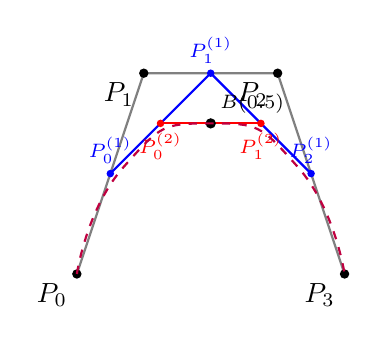
\begin{tikzpicture}[scale=0.85,>=stealth]
  % Control points
  \coordinate (P0) at (0,0);
  \coordinate (P1) at (1,3);
  \coordinate (P2) at (3,3);
  \coordinate (P3) at (4,0);

  % Level-1 points (t = 0.5 for visual clarity)
  \coordinate (Q0) at (0.5,1.5);
  \coordinate (Q1) at (2,3);
  \coordinate (Q2) at (3.5,1.5);

  % Level-2 points
  \coordinate (R0) at (1.25,2.25);
  \coordinate (R1) at (2.75,2.25);

  % Level-3 (B(0.5))
  \coordinate (B)  at (2,2.25);

  % Control polygon
  \draw[thick,gray] (P0)--(P1)--(P2)--(P3);
  \foreach \p/\l in {P0/$P_0$,P1/$P_1$,P2/$P_2$,P3/$P_3$}
     {\fill (\p) circle (2pt); \node[below left] at (\p) {\l};}

  % Level 1
  \draw[blue,thick] (Q0)--(Q1)--(Q2);
  \foreach \p/\l in {Q0/$P_0^{(1)}$,Q1/$P_1^{(1)}$,Q2/$P_2^{(1)}$}
     {\fill[blue] (\p) circle (1.6pt); \node[above,blue,font=\scriptsize] at (\p) {\l};}

  % Level 2
  \draw[red,thick] (R0)--(R1);
  \foreach \p/\l in {R0/$P_0^{(2)}$,R1/$P_1^{(2)}$}
     {\fill[red] (\p) circle (1.6pt); \node[below,red,font=\scriptsize] at (\p) {\l};}

  % B(t)
  \fill[black] (B) circle (2.2pt);
  \node[above right,font=\scriptsize] at (B) {$B(0.5)$};

  % Approximate curve sketch
  \draw[dashed,thick,purple] plot[smooth,tension=1] coordinates {(P0)(0.7,1.6)(2,2.25)(3.3,1.6)(P3)};
\end{tikzpicture}
\end{center}
\textbf{EN:} grey = control polygon; blue = level-1 polygon; red = level-2 segment; black = $B(t)$; dashed purple = the actual Bezier curve.

\switchcolumn

\subsection*{4.4* Hình minh hoạ De Casteljau}

\begin{center}
\textit{(Hình bên cột trái)}
\end{center}

\textbf{VI:} xám = control polygon gốc; xanh = đa giác mức 1 (lấy điểm chia $t$ trên mỗi cạnh); đỏ = đoạn mức 2; đen = điểm $B(t)$; tím nét đứt = đường cong Bezier thực sự.\\
Quan sát: các đoạn nối các điểm trung gian (đa giác xanh, đỏ) ngày càng tiệm cận đường cong; đa giác mức 1 thậm chí \emph{tiếp xúc} với curve tại $B(t)$ (đó là tiếp tuyến của curve tại $t$).

\medskip
\textbf{Tổng kết các mức:}
\begin{itemize}[leftmargin=*,nosep]
  \item Mức 0: $n{+}1$ điểm gốc $P_0,\dots,P_n$.
  \item Mức 1: $n$ điểm $P_i^{(1)}$ -- mỗi điểm chia một cạnh.
  \item Mức $k$: $n{+}1{-}k$ điểm.
  \item Mức $n$: \emph{một} điểm duy nhất $=B(t)$.
\end{itemize}
\textbf{Mẹo thi:} với $n=3$, kẻ \emph{tam giác De Casteljau} 4 cột $\to$ 3 cột $\to$ 2 cột $\to$ 1 cột. Khi $t=0.5$, các trọng số đối xứng nên tính nhanh hơn.

\switchcolumn*

% ---------------------------------------------------------------------
% 4.5  BEZIER SURFACE
% ---------------------------------------------------------------------
\subsection*{4.5 Bezier Surface (Tensor Product)}

A \textbf{Bezier surface (patch)} of bi-degree $(m,n)$ is defined by an $(m{+}1)\times(n{+}1)$ grid of control points $P_{ij}$ (the \emph{control net}):
\[
S(u,v)=\sum_{i=0}^{m}\sum_{j=0}^{n}B_i^{\,m}(u)\,B_j^{\,n}(v)\,P_{ij},
\quad (u,v)\in[0,1]^{2}.
\]

\textbf{Properties.}
\begin{itemize}[leftmargin=*,nosep]
  \item Corner interpolation: $S(0,0)=P_{00}$, $S(1,0)=P_{m0}$, $S(0,1)=P_{0n}$, $S(1,1)=P_{mn}$.
  \item Convex hull of the control net contains the patch.
  \item Affine invariance.
  \item \emph{Isoparametric curves} $u=u_0$ or $v=v_0$ are themselves Bezier curves of degree $n$ (resp.\ $m$).
  \item \emph{Boundary curves} are the four Bezier curves through the four edges of the control net.
  \item Tangent at corner $(0,0)$ along $u$: $S_u(0,0)=m(P_{10}-P_{00})$; along $v$: $S_v(0,0)=n(P_{01}-P_{00})$.
\end{itemize}

\textbf{Bicubic patch} ($m=n=3$): $4\times 4=16$ control points -- the workhorse of CAD/animation.

\begin{center}
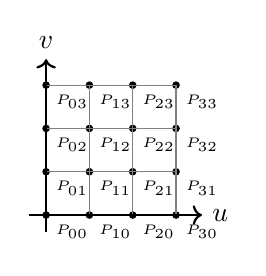
\begin{tikzpicture}[scale=0.55]
  \foreach \i in {0,1,2,3}{
    \foreach \j in {0,1,2,3}{
      \fill (\i,\j) circle (2.5pt);
      \node[font=\tiny,below right] at (\i,\j) {$P_{\i\j}$};
    }
  }
  % grid lines
  \foreach \i in {0,1,2,3}{ \draw[gray] (\i,0)--(\i,3); \draw[gray] (0,\i)--(3,\i); }
  \draw[->,thick] (-0.4,0)--(3.6,0) node[right]{$u$};
  \draw[->,thick] (0,-0.4)--(0,3.6) node[above]{$v$};
\end{tikzpicture}
\end{center}

\switchcolumn

\subsection*{4.5 Mặt Bezier (tích tensor)}

\textbf{Mặt (patch) Bezier} bậc $(m,n)$ được xác định bởi \emph{lưới control net} kích thước $(m{+}1){\times}(n{+}1)$:
\[
S(u,v)=\sum_{i=0}^{m}\sum_{j=0}^{n}B_i^{\,m}(u)B_j^{\,n}(v)P_{ij}.
\]

\textbf{Tính chất.}
\begin{itemize}[leftmargin=*,nosep]
  \item Nội suy 4 góc: $S(0,0)=P_{00}$, $S(1,0)=P_{m0}$, $S(0,1)=P_{0n}$, $S(1,1)=P_{mn}$.
  \item Nằm trong bao lồi của control net.
  \item Bất biến affine.
  \item \emph{Đường isoparametric} $u=u_0$ hoặc $v=v_0$ là đường cong Bezier bậc $n$ (hoặc $m$).
  \item \emph{4 đường biên} là 4 curve Bezier nằm trên 4 cạnh của control net.
  \item Tiếp tuyến tại góc $(0,0)$: $S_u=m(P_{10}-P_{00})$, $S_v=n(P_{01}-P_{00})$.
\end{itemize}

\textbf{Bicubic patch} ($m=n=3$): 16 control point -- dạng phổ biến nhất trong CAD/animation, mô phỏng vải, hoạt cảnh nhân vật...

\medskip
\textbf{Đường iso} có nghĩa là cố định một biến (vd $u=0.3$) rồi cho biến kia chạy. Đó vẫn là Bezier curve nên có thể áp dụng lại De Casteljau.

\switchcolumn*

% ---------------------------------------------------------------------
% 4.6  DE CASTELJAU ON SURFACES
% ---------------------------------------------------------------------
\subsection*{4.6 De Casteljau on Surfaces}

To compute $S(u,v)$ for a $(m{+}1)\times(n{+}1)$ control net:

\textbf{Method 1 (rows first).}
\begin{enumerate}[leftmargin=*,nosep]
  \item For each row $i=0,\dots,m$, run de Casteljau on $(P_{i0},\dots,P_{in})$ at parameter $v$ $\Rightarrow$ point $Q_i$.
  \item Run de Casteljau on $(Q_0,\dots,Q_m)$ at parameter $u$ $\Rightarrow$ $S(u,v)$.
\end{enumerate}
\textbf{Method 2 (columns first).} Swap the order: first reduce columns at $u$, then the resulting $(n{+}1)$ points at $v$. Same answer (tensor-product structure commutes).

\medskip
\textbf{Cost.} $O(m^{2}n+mn^{2})$ multiplications -- dominated by the smaller of the two passes. For bicubic ($m=n=3$): $4\times 6+4\times 6=48$ scalar lerps per coordinate $\approx$ trivial.

\begin{algorithm}[H]
\small
\DontPrintSemicolon
\KwIn{control net $P_{ij}$, $i{=}0..m,\,j{=}0..n$; $(u,v)$}
\For{$i\gets 0$ \KwTo $m$}{
   $Q_i \gets$ \textsc{DeCasteljau}$\bigl(P_{i0},\dots,P_{in};\,v\bigr)$\;
}
\Return \textsc{DeCasteljau}$(Q_0,\dots,Q_m;\,u)$\;
\caption{De Casteljau (surface, row-first)}
\end{algorithm}

\switchcolumn

\subsection*{4.6 De Casteljau cho mặt}

Để tính $S(u,v)$ trên control net $(m{+}1)\times(n{+}1)$:

\textbf{Cách 1 (theo hàng trước).}
\begin{enumerate}[leftmargin=*,nosep]
  \item Với mỗi hàng $i=0,\dots,m$: chạy De Casteljau trên $(P_{i0},\dots,P_{in})$ tại $v$, được điểm $Q_i$.
  \item Chạy De Casteljau trên $(Q_0,\dots,Q_m)$ tại $u$, được $S(u,v)$.
\end{enumerate}

\textbf{Cách 2 (theo cột trước).} Đảo thứ tự: rút cột trước (theo $u$), được $n{+}1$ điểm; rồi rút theo $v$. Kết quả \emph{giống nhau} do cấu trúc tensor.

\medskip
\textbf{Lựa chọn:} dùng \emph{cách hàng trước} nếu $m<n$ (ít vòng lặp ngoài), ngược lại dùng \emph{cách cột trước}. Với bicubic thì gần như tương đương.

\medskip
\textbf{Quan trọng cho thi:} vì cách nào cũng đúng, hãy chọn cách \emph{tận dụng được} các giá trị tròn (vd nếu $v=0.5$ thì giảm hàng trước cho dễ tính nhẩm).

\switchcolumn*

% ---------------------------------------------------------------------
% 4.7  WORKED EXAMPLE BEZIER SURFACE
% ---------------------------------------------------------------------
\subsection*{4.7 Worked Example --- Bezier Surface at $(u,v)=(0.5,0.5)$}

\textbf{Setup (biquadratic, $m=n=2$).} Use a $3\times 3$ control net (only the $z$-coordinate varies, $x=i$, $y=j$):
\[
P_{ij}=(i,\,j,\,h_{ij}),\qquad h=\begin{pmatrix}0&1&0\\1&3&1\\0&1&0\end{pmatrix},
\]
i.e.\ a small "tent" peaking at the centre. Compute $S(0.5,0.5)$.

\medskip
\textbf{Step 1 -- reduce each row at $v=0.5$ (quadratic De Casteljau).}

For row $i$, control points are $h_{i0},h_{i1},h_{i2}$; for $v=0.5$:
\[
Q_i = \tfrac14 h_{i0}+\tfrac12 h_{i1}+\tfrac14 h_{i2}.
\]
\begin{itemize}[leftmargin=*,nosep]
  \item Row 0: $Q_0^h=\tfrac14\cdot0+\tfrac12\cdot1+\tfrac14\cdot0=\tfrac12$. So $Q_0=(0,\,1,\,0.5)$.
  \item Row 1: $Q_1^h=\tfrac14\cdot1+\tfrac12\cdot3+\tfrac14\cdot1=\tfrac14+\tfrac32+\tfrac14=2$. So $Q_1=(1,\,1,\,2)$.
  \item Row 2: $Q_2^h=\tfrac14\cdot0+\tfrac12\cdot1+\tfrac14\cdot0=\tfrac12$. So $Q_2=(2,\,1,\,0.5)$.
\end{itemize}
(Note the $y$-coords come out as $1$ because $\tfrac14\cdot 0+\tfrac12\cdot 1+\tfrac14\cdot 2=1$.)

\textbf{Step 2 -- reduce $(Q_0,Q_1,Q_2)$ at $u=0.5$.}
\[
S=\tfrac14 Q_0+\tfrac12 Q_1+\tfrac14 Q_2.
\]
\begin{align*}
x &: \tfrac14\cdot 0+\tfrac12\cdot 1+\tfrac14\cdot 2 = 1,\\
y &: \tfrac14\cdot 1+\tfrac12\cdot 1+\tfrac14\cdot 1 = 1,\\
z &: \tfrac14\cdot 0.5+\tfrac12\cdot 2+\tfrac14\cdot 0.5 = 0.125+1+0.125=1.25.
\end{align*}
\[
\boxed{\,S(0.5,0.5)=(1,\,1,\,1.25)\,}.
\]

\medskip
\textbf{Sanity check (Bernstein direct).} For $n=m=2$ the Bernstein weights at $(0.5,0.5)$ are $(\tfrac14,\tfrac12,\tfrac14)\otimes(\tfrac14,\tfrac12,\tfrac14)$, the $z$-sum equals
\[
\tfrac{1}{16}\!\sum_{ij}w_{ij}h_{ij}\quad\text{with}\quad w=\begin{pmatrix}1&2&1\\2&4&2\\1&2&1\end{pmatrix}.
\]
$\sum w_{ij}h_{ij}=1\!\cdot\!0+2\!\cdot\!1+1\!\cdot\!0+2\!\cdot\!1+4\!\cdot\!3+2\!\cdot\!1+1\!\cdot\!0+2\!\cdot\!1+1\!\cdot\!0$
$=0+2+0+2+12+2+0+2+0=20$. So $z=20/16=1.25$. \checkmark

\switchcolumn

\subsection*{4.7 Ví dụ mặt Bezier tại $(u,v)=(0.5,0.5)$}

\textbf{Dữ liệu (bậc $2{\times}2$).} Lưới $3\times 3$, $x=i,y=j$, độ cao $h_{ij}$ như bảng:
\[
h=\begin{pmatrix}0&1&0\\1&3&1\\0&1&0\end{pmatrix}.
\]
Tính $S(0.5,0.5)$.

\textbf{Bước 1 -- giảm hàng tại $v=0.5$:}
trọng số bậc 2 là $(\tfrac14,\tfrac12,\tfrac14)$.
\begin{itemize}[leftmargin=*,nosep]
  \item Hàng 0: $z=\tfrac14(0)+\tfrac12(1)+\tfrac14(0)=0.5\Rightarrow Q_0=(0,1,0.5)$.
  \item Hàng 1: $z=\tfrac14(1)+\tfrac12(3)+\tfrac14(1)=2\Rightarrow Q_1=(1,1,2)$.
  \item Hàng 2: $z=0.5\Rightarrow Q_2=(2,1,0.5)$.
\end{itemize}

\textbf{Bước 2 -- giảm $(Q_0,Q_1,Q_2)$ tại $u=0.5$:}
\[
S=\tfrac14 Q_0+\tfrac12 Q_1+\tfrac14 Q_2 = (1,1,1.25).
\]
\[
\boxed{S(0.5,0.5)=(1,1,1.25)}.
\]

\textbf{Kiểm tra.} Theo Bernstein 2D, các trọng số là tích Kronecker
$(\tfrac14,\tfrac12,\tfrac14){\otimes}(\tfrac14,\tfrac12,\tfrac14)$, ma trận trọng số $\frac{1}{16}\begin{psmallmatrix}1&2&1\\2&4&2\\1&2&1\end{psmallmatrix}$. Nhân với ma trận $h$ rồi cộng tổng: $20/16=1.25$ \checkmark.

\medskip
\textbf{Mở rộng cho bicubic:} cũng tương tự nhưng có 4 hàng, mỗi hàng giảm theo De Casteljau bậc 3. Sau đó còn 4 điểm $Q_0..Q_3$, giảm tiếp 1 lần De Casteljau bậc 3 nữa $\to$ ra $S(u,v)$.

\switchcolumn*

% ---------------------------------------------------------------------
% 4.8  OTHER PARAMETRIC CURVES
% ---------------------------------------------------------------------
\subsection*{4.8 Other Parametric Curves (Context)}

\begin{itemize}[leftmargin=*,nosep]
  \item \textbf{Hermite}: defined by 2 endpoints $P_0,P_1$ and 2 tangents $T_0,T_1$. Cubic: $H(t)=h_{00}P_0+h_{10}T_0+h_{01}P_1+h_{11}T_1$ with the four Hermite basis polynomials $h_{00}=2t^3-3t^2+1$ etc.
  \item \textbf{Catmull--Rom}: an \emph{interpolating} spline through control points; tangent at $P_i$ is $\tfrac12(P_{i+1}-P_{i-1})$. Local control, $C^1$.
  \item \textbf{B-splines}: piecewise polynomials with \emph{knot vector}; only $k{+}1$ basis functions are non-zero on a span $\Rightarrow$ \emph{local control} (move one CP and only nearby curve changes). Bezier is the special case of a single non-uniform knot vector $\{0,\dots,0,1,\dots,1\}$.
  \item \textbf{NURBS} = Non-Uniform Rational B-Splines. Adds positive weights $w_i$:
        $C(t)=\dfrac{\sum w_i N_i^{p}(t) P_i}{\sum w_i N_i^{p}(t)}$. Can represent conics exactly (circle, ellipse).
\end{itemize}

\textbf{Comparison.}
\begin{center}\scriptsize
\begin{tabular}{@{}lcccc@{}}\toprule
 & Interp.? & Local ctrl? & Tangent ctl? & Conics? \\\midrule
Bezier         & endpoints only & no  & via $P_1,P_{n-1}$ & no \\
Hermite        & endpoints      & no  & yes (explicit)    & no \\
Catmull--Rom   & yes (all CP)   & yes & no (auto)         & no \\
B-spline       & no             & yes & no                & no \\
NURBS          & no (ctrl + $w$)& yes & no                & yes \\\bottomrule
\end{tabular}
\end{center}

\switchcolumn

\subsection*{4.8 Các loại đường cong tham số khác}

\begin{itemize}[leftmargin=*,nosep]
  \item \textbf{Hermite}: xác định bởi 2 điểm đầu mút + 2 tiếp tuyến. Bậc 3, hữu ích khi đã có thông tin tiếp tuyến.
  \item \textbf{Catmull--Rom}: spline \emph{nội suy} đi qua các control point; tiếp tuyến tại $P_i$ tự động tính $=\tfrac12(P_{i+1}-P_{i-1})$. Có local control, liên tục $C^1$.
  \item \textbf{B-spline}: đa thức piecewise, có \emph{knot vector}; mỗi hàm cơ sở chỉ ảnh hưởng cục bộ $\Rightarrow$ \emph{điều khiển địa phương}. Bezier là trường hợp đặc biệt với knot $\{0,\dots,0,1,\dots,1\}$.
  \item \textbf{NURBS} = B-spline \emph{hữu tỉ + không đều}; có trọng số $w_i$, biểu diễn được đường tròn / ellipse \emph{chính xác}, là chuẩn trong CAD.
\end{itemize}

\textbf{So sánh.}
\begin{center}\scriptsize
\begin{tabular}{@{}lcccc@{}}\toprule
 & Nội suy? & Local? & Tiếp tuyến? & Conic? \\\midrule
Bezier         & 2 đầu mút       & không & qua $P_1,P_{n-1}$ & không \\
Hermite        & 2 đầu mút       & không & có (tường minh)    & không \\
Catmull--Rom   & qua mọi CP      & có    & tự động            & không \\
B-spline       & không           & có    & không              & không \\
NURBS          & không (CP $+w$) & có    & không              & có \\\bottomrule
\end{tabular}
\end{center}

\switchcolumn*

% ---------------------------------------------------------------------
% 4.9  SUBDIVISION & DERIVATIVE & DEGREE ELEVATION
% ---------------------------------------------------------------------
\subsection*{4.9 Subdivision, Derivatives, Degree Elevation}

\textbf{Subdivision (free from De Casteljau).} Running de Casteljau at $t$ \emph{produces}, as a side product, the control polygons of the two halves of the curve:
\begin{align*}
\text{Left half:}\;& P_0^{(0)},\,P_0^{(1)},\,P_0^{(2)},\,\dots,\,P_0^{(n)},\\
\text{Right half:}\;& P_0^{(n)},\,P_1^{(n-1)},\,P_2^{(n-2)},\,\dots,\,P_n^{(0)}.
\end{align*}
The two halves together reproduce the original curve; this is the basis of \emph{adaptive rendering} (recursively subdivide until the polygon is "flat enough").

\textbf{Derivative.} The derivative of a degree-$n$ Bezier curve is itself a degree-$(n{-}1)$ Bezier curve on the \emph{forward differences}:
\[
B'(t)=n\sum_{i=0}^{n-1}B_i^{\,n-1}(t)\,(P_{i+1}-P_i).
\]
At endpoints: $B'(0)=n(P_1-P_0)$, $B'(1)=n(P_n-P_{n-1})$ (already noted).

\textbf{Degree elevation.} A degree-$n$ Bezier with points $P_0,\dots,P_n$ is also a degree-$(n{+}1)$ Bezier with $n{+}2$ points $P_i'$:
\[
P_i'=\tfrac{i}{n+1}P_{i-1}+\Bigl(1-\tfrac{i}{n+1}\Bigr)P_i,\quad i=0,\dots,n+1,
\]
(with $P_{-1}, P_{n+1}$ interpreted via the boundary cases $P_0'=P_0$, $P_{n+1}'=P_n$). Useful to make two Bezier patches/curves have matching degrees before joining.

\textbf{$C^1$ joining of two cubic Bezier curves} with control points $\{P_0,P_1,P_2,P_3\}$ then $\{Q_0,Q_1,Q_2,Q_3\}$:
need $Q_0=P_3$ ($C^0$) and $Q_1-Q_0 = P_3-P_2$ ($C^1$), i.e.\ $Q_1=2P_3-P_2$.

\switchcolumn

\subsection*{4.9 Phân chia, Đạo hàm, Nâng bậc}

\textbf{Phân chia (subdivision)} miễn phí từ De Casteljau. Khi chạy thuật toán tại $t$, các điểm trung gian \emph{tự sinh ra} 2 control polygon mới:
\[
\text{Trái: } P_0^{(0)},P_0^{(1)},\dots,P_0^{(n)};\quad
\text{Phải: } P_0^{(n)},P_1^{(n-1)},\dots,P_n^{(0)}.
\]
Hợp lại tái tạo đúng curve gốc -- là cơ sở để \emph{vẽ thích nghi} (đệ quy cho tới khi polygon đủ "phẳng" thì vẽ luôn các đoạn thẳng).

\textbf{Đạo hàm.} Đạo hàm của Bezier bậc $n$ là Bezier bậc $n{-}1$ trên \emph{sai phân}:
\[
B'(t)=n\sum_{i=0}^{n-1}B_i^{\,n-1}(t)(P_{i+1}-P_i).
\]
Ở đầu mút: $B'(0)=n(P_1-P_0)$, $B'(1)=n(P_n-P_{n-1})$.

\textbf{Nâng bậc (degree elevation).} Curve bậc $n$ có thể viết lại thành bậc $n{+}1$ với $n{+}2$ điểm
\[
P_i'=\tfrac{i}{n+1}P_{i-1}+\Bigl(1-\tfrac{i}{n+1}\Bigr)P_i.
\]
Hữu ích khi cần \emph{khớp bậc} 2 đoạn curve trước khi nối.

\textbf{Nối $C^1$ giữa 2 curve bậc 3} $\{P_i\}$ và $\{Q_i\}$:
$Q_0=P_3$ (cùng điểm), $Q_1=2P_3-P_2$ (cùng tiếp tuyến).

\switchcolumn*

% ---------------------------------------------------------------------
% 4.10  EXAM STRATEGIES
% ---------------------------------------------------------------------
\subsection*{4.10 Exam-Style Problems \& Strategies}

\begin{enumerate}[leftmargin=*,nosep]
  \item \emph{"Compute $B(t)$ at given $t$"} $\to$ De Casteljau (faster, fewer arithmetic mistakes than Bernstein for one $t$). Always lay out the triangle.
  \item \emph{"Compute $S(u,v)$"} $\to$ row-wise De Casteljau then column-wise. Decide order based on which $u$/$v$ is "nicer".
  \item \emph{"Subdivide at $t$"} $\to$ run De Casteljau, then read off the left/right control polygons (\S 4.9).
  \item \emph{"Tangent at endpoint"} $\to$ $B'(0)=n(P_1-P_0)$ or $B'(1)=n(P_n-P_{n-1})$.
  \item \emph{"Match $C^0/C^1$ between curves"} $\to$ shared endpoint + collinear adjacent control points with correct length ratio.
  \item \emph{"Verify a property"} (convex hull, partition of unity, etc.) $\to$ cite Bernstein property; show $\sum B_i^{n}(t)=1$ via $((1-t)+t)^n=1$.
  \item \emph{"Convert Bezier $\to$ monomial"} (rare): multiply out $\sum\binom{n}{i}(1-t)^{n-i}t^i P_i$ symbolically.
  \item \emph{"Pick t to minimise computation"}: $t=0,1,\tfrac12$ are easiest. $t=\tfrac13,\tfrac23$ keep things in thirds.
\end{enumerate}

\textbf{Common pitfalls.}
\begin{itemize}[leftmargin=*,nosep]
  \item Forgetting that weights are $(1-t)$ for the \emph{left} point and $t$ for the \emph{right} -- not the other way around.
  \item Using $\binom{n}{i}$ wrong (e.g.\ $\binom{3}{1}=3$ not $1$).
  \item In a surface problem, mixing up $u$/$v$ -- always label rows vs columns first.
  \item Forgetting that $B(0)=P_0$, $B(1)=P_n$ (not $P_1,\dots,P_{n-1}$).
\end{itemize}

\switchcolumn

\subsection*{4.10 Dạng bài thi \& Chiến thuật}

\begin{enumerate}[leftmargin=*,nosep]
  \item \emph{"Tính $B(t)$ tại $t$ cho trước"} $\to$ dùng De Casteljau (ít lỗi số học hơn Bernstein cho một giá trị $t$). Vẽ bảng tam giác rõ ràng.
  \item \emph{"Tính $S(u,v)$"} $\to$ giảm hàng theo $v$ trước, rồi giảm theo $u$ (hoặc ngược lại). Chọn thứ tự sao cho $t$ nào "đẹp" thì làm cuối.
  \item \emph{"Phân chia tại $t$"} $\to$ chạy De Casteljau, đọc 2 polygon ở 2 cạnh tam giác (\S 4.9).
  \item \emph{"Tiếp tuyến tại đầu mút"} $\to$ $B'(0)=n(P_1-P_0)$ hoặc $B'(1)=n(P_n-P_{n-1})$.
  \item \emph{"Nối $C^0/C^1$"} $\to$ trùng đầu mút + 3 điểm liền kề thẳng hàng, tỉ lệ độ dài hợp lý.
  \item \emph{"Chứng minh tính chất"} $\to$ trích dẫn Bernstein; tổng đa thức Bernstein $=((1-t)+t)^n=1$.
\end{enumerate}

\textbf{Lỗi hay gặp.}
\begin{itemize}[leftmargin=*,nosep]
  \item Lẫn trọng số: $(1-t)$ đi với điểm \emph{trái}, $t$ đi với điểm \emph{phải}.
  \item Sai $\binom{n}{i}$ -- nên chép luôn dòng Pascal trước khi tính.
  \item Trong bài surface, lẫn vai trò $u$/$v$ -- ghi rõ $i$ là chỉ số hàng, $j$ là cột.
  \item Nhớ $B(0)=P_0, B(1)=P_n$ -- KHÔNG đi qua các CP ở giữa.
\end{itemize}

\switchcolumn*

% ---------------------------------------------------------------------
% 4.11  BERNSTEIN TABLE
% ---------------------------------------------------------------------
\subsection*{4.11 Bernstein Coefficient Tables}

\textbf{Quadratic ($n=2$):} weights $((1-t)^2,\,2(1-t)t,\,t^2)$.
\begin{center}\small
\begin{tabular}{c|ccc|c}
$t$ & $B_0^2$ & $B_1^2$ & $B_2^2$ & sum \\\midrule
$0.25$ & $9/16=0.5625$ & $6/16=0.3750$ & $1/16=0.0625$ & 1\\
$0.50$ & $1/4=0.25$    & $1/2=0.50$    & $1/4=0.25$    & 1\\
$0.75$ & $1/16=0.0625$ & $6/16=0.3750$ & $9/16=0.5625$ & 1\\
\end{tabular}
\end{center}

\textbf{Cubic ($n=3$):} weights $((1-t)^3,\,3(1-t)^2t,\,3(1-t)t^2,\,t^3)$.
\begin{center}\small
\begin{tabular}{c|cccc|c}
$t$ & $B_0^3$ & $B_1^3$ & $B_2^3$ & $B_3^3$ & sum \\\midrule
$0.25$ & $27/64=0.421875$ & $27/64=0.421875$ & $9/64=0.140625$  & $1/64=0.015625$ & 1\\
$0.50$ & $1/8=0.125$      & $3/8=0.375$      & $3/8=0.375$      & $1/8=0.125$     & 1\\
$0.75$ & $1/64=0.015625$  & $9/64=0.140625$  & $27/64=0.421875$ & $27/64=0.421875$& 1\\
$1/3$  & $8/27\approx0.296$ & $12/27\approx0.444$ & $6/27\approx0.222$ & $1/27\approx0.037$ & 1\\
$2/3$  & $1/27$ & $6/27$ & $12/27$ & $8/27$ & 1\\
\end{tabular}
\end{center}

\textbf{Quartic ($n=4$) at $t=0.5$:}\\
$B^4=(\tfrac{1}{16},\tfrac{4}{16},\tfrac{6}{16},\tfrac{4}{16},\tfrac{1}{16})=(.0625,.25,.375,.25,.0625)$.

\textbf{Quintic ($n=5$) at $t=0.5$:}
$B^5=(1/32,\,5/32,\,10/32,\,10/32,\,5/32,\,1/32)$.

\textbf{Symmetry:} $B_i^n(t)=B_{n-i}^{\,n}(1-t)$ -- so the row at $t=0.75$ is the row at $t=0.25$ reversed (visible above).

\switchcolumn

\subsection*{4.11 Bảng tra hệ số Bernstein}

\textbf{Bậc 2:} trọng số $((1-t)^2,2(1-t)t,t^2)$.
\begin{center}\small
\begin{tabular}{c|ccc|c}
$t$ & $B_0^2$ & $B_1^2$ & $B_2^2$ & tổng \\\midrule
$0.25$ & $0.5625$ & $0.3750$ & $0.0625$ & 1\\
$0.50$ & $0.25$ & $0.50$ & $0.25$ & 1\\
$0.75$ & $0.0625$ & $0.3750$ & $0.5625$ & 1\\
\end{tabular}
\end{center}

\textbf{Bậc 3:}
\begin{center}\small
\begin{tabular}{c|cccc|c}
$t$ & $B_0^3$ & $B_1^3$ & $B_2^3$ & $B_3^3$ & tổng\\\midrule
$0.25$ & $0.421875$ & $0.421875$ & $0.140625$ & $0.015625$ & 1\\
$0.50$ & $0.125$ & $0.375$ & $0.375$ & $0.125$ & 1\\
$0.75$ & $0.015625$ & $0.140625$ & $0.421875$ & $0.421875$& 1\\
$1/3$  & $8/27$ & $12/27$ & $6/27$ & $1/27$ & 1\\
$2/3$  & $1/27$ & $6/27$ & $12/27$ & $8/27$ & 1\\
\end{tabular}
\end{center}

\textbf{Bậc 4 tại $t=0.5$:}
$(1,4,6,4,1)/16=(0.0625,0.25,0.375,0.25,0.0625)$.

\textbf{Bậc 5 tại $t=0.5$:}
$(1,5,10,10,5,1)/32$.

\textbf{Đối xứng:} $B_i^n(t)=B_{n-i}^{\,n}(1-t)$. Vì vậy hàng $t=0.75$ là hàng $t=0.25$ đảo chiều -- tiết kiệm thời gian khi tra bảng.

\textbf{Mẹo nhớ:} hệ số bậc $n$ là hàng $n$ của tam giác Pascal; phần $(1-t)^{n-i}t^i$ chính là "phép phối $n-i$ lần $1-t$ và $i$ lần $t$".

\switchcolumn*

% ---------------------------------------------------------------------
% 4.12  ONE-PAGE SUMMARY (FORMULA SHEET)
% ---------------------------------------------------------------------
\subsection*{4.12 One-Glance Formula Box}

\fbox{\parbox{0.95\columnwidth}{\small
\textbf{Bezier curve:}\;$B(t)=\sum_{i=0}^{n}\binom{n}{i}(1-t)^{n-i}t^{i}P_i$.\\[2pt]
\textbf{Bernstein:}\;$B_i^n(t)=\binom{n}{i}(1-t)^{n-i}t^i$,\;$\sum_i B_i^n(t)=1$.\\[2pt]
\textbf{De Casteljau:}\;$P_i^{(k)}=(1-t)P_i^{(k-1)}+tP_{i+1}^{(k-1)}$;\;$B(t)=P_0^{(n)}$.\\[2pt]
\textbf{Tangent:}\;$B'(0)=n(P_1-P_0)$,\;$B'(1)=n(P_n-P_{n-1})$.\\[2pt]
\textbf{Derivative curve:}\;$B'(t)=n\sum B_i^{n-1}(t)(P_{i+1}-P_i)$.\\[2pt]
\textbf{Degree elevation:}\;$P_i'=\tfrac{i}{n+1}P_{i-1}+(1-\tfrac{i}{n+1})P_i$.\\[2pt]
\textbf{Subdivision halves:}\\
\hspace*{6pt}left\;$=\{P_0^{(0)},P_0^{(1)},\dots,P_0^{(n)}\}$,\\
\hspace*{6pt}right\;$=\{P_0^{(n)},P_1^{(n-1)},\dots,P_n^{(0)}\}$.\\[2pt]
\textbf{Surface:}\;$S(u,v)=\sum_{i,j}B_i^m(u)B_j^n(v)P_{ij}$.\\[2pt]
\textbf{Surface eval:}\;rows-at-$v$ then column-at-$u$ (or vice-versa).\\[2pt]
\textbf{Corner:}\;$S(0,0)=P_{00}$, etc.\\[2pt]
\textbf{Surface tangents at $(0,0)$:}\;$S_u=m(P_{10}-P_{00})$,\;$S_v=n(P_{01}-P_{00})$.
}}

\switchcolumn

\subsection*{4.12 Khung công thức tóm tắt}

\fbox{\parbox{0.95\columnwidth}{\small
\textbf{Curve Bezier:}\;$B(t)=\sum\binom{n}{i}(1-t)^{n-i}t^{i}P_i$.\\[2pt]
\textbf{Bernstein:}\;$B_i^n=\binom{n}{i}(1-t)^{n-i}t^i$,\;tổng $=1$.\\[2pt]
\textbf{De Casteljau:}\;$P_i^{(k)}=(1-t)P_i^{(k-1)}+tP_{i+1}^{(k-1)}$.\\[2pt]
\textbf{Tiếp tuyến đầu mút:}\;$n(P_1-P_0)$ và $n(P_n-P_{n-1})$.\\[2pt]
\textbf{Đạo hàm:}\;$B'(t)=n\sum B_i^{n-1}(t)(P_{i+1}-P_i)$.\\[2pt]
\textbf{Nâng bậc:}\;$P_i'=\tfrac{i}{n+1}P_{i-1}+(1-\tfrac{i}{n+1})P_i$.\\[2pt]
\textbf{Phân chia:} polygon trái\;$\{P_0^{(0)},\dots,P_0^{(n)}\}$, phải\;$\{P_0^{(n)},\dots,P_n^{(0)}\}$.\\[2pt]
\textbf{Mặt:}\;$S(u,v)=\sum B_i^m(u)B_j^n(v)P_{ij}$.\\[2pt]
\textbf{Tính $S$:}\;giảm hàng tại $v$ rồi giảm cột tại $u$ (hoặc ngược lại).\\[2pt]
\textbf{Góc:}\;$S(0,0)=P_{00},\,S(1,0)=P_{m0},\,S(0,1)=P_{0n},\,S(1,1)=P_{mn}$.\\[2pt]
\textbf{Tiếp tuyến tại $(0,0)$:}\;$m(P_{10}-P_{00})$ và $n(P_{01}-P_{00})$.\\[2pt]
\textbf{Mẹo phòng thi:} luôn vẽ \emph{tam giác De Casteljau}, đánh dấu trọng số $1{-}t$ (trái) và $t$ (phải).
}}

\end{paracol}

% =====================================================================
% End of section 4
% =====================================================================


\vfill\hrule\vspace{4pt}

% =====================================================================
% 06_bicubic_example.tex -- Worked Example: Bicubic Bezier Surface
% Compute S(0.5, 0.5) on a 4x4 control net step-by-step.
% Bilingual EN | VI cheatsheet section for IT516 Advanced Computer Graphics
% =====================================================================

\begin{paracol}{2}

% =====================================================================
% ENGLISH COLUMN
% =====================================================================
\section*{6.\ Worked Example: Bicubic Bezier Surface (4$\times$4) at $(u,v)=(0.5,0.5)$}

\subsection*{6.1 Setup --- the 4$\times$4 Control Net}

A \textbf{bicubic Bezier surface} (degree 3 in both $u$ and $v$) needs a $4\times 4$ control net $\{P_{ij}\}_{i,j=0}^{3}$. We use the following ``hill / tent'' net (rows $i$ run along $u$, columns $j$ run along $v$):
\[
\renewcommand{\arraystretch}{1.1}
\begin{array}{c|cccc}
 & j=0 & j=1 & j=2 & j=3 \\\hline
i{=}0 & (0,0,0) & (1,0,1) & (2,0,1) & (3,0,0) \\
i{=}1 & (0,1,1) & (1,1,3) & (2,1,3) & (3,1,1) \\
i{=}2 & (0,2,1) & (1,2,3) & (2,2,3) & (3,2,1) \\
i{=}3 & (0,3,0) & (1,3,1) & (2,3,1) & (3,3,0)
\end{array}
\]
The $(x,y)$ are on the integer grid; only the $z$-component varies (saddle/tent peak in the centre). We want $S(0.5,\,0.5)$.

The surface formula:
\[
S(u,v)=\sum_{i=0}^{3}\sum_{j=0}^{3} B_i^3(u)\,B_j^3(v)\,P_{ij}.
\]
We will compute $S(0.5,0.5)$ \textbf{three ways} and check they match.

% ---------------------------------------------------------------------
\subsection*{6.2 Method 1 --- Row-first De Casteljau}

\textbf{Step A.} For each row $i$, run De Casteljau in $v$ at $v=0.5$ on the four points $P_{i0},P_{i1},P_{i2},P_{i3}$ to obtain $Q_i$.

\textbf{Row 0:} $(0,0,0),(1,0,1),(2,0,1),(3,0,0)$
\begin{align*}
\text{L1: }& \tfrac{1}{2}(P_{00}{+}P_{01})=(0.5,0,0.5)\\
           & \tfrac{1}{2}(P_{01}{+}P_{02})=(1.5,0,1)\\
           & \tfrac{1}{2}(P_{02}{+}P_{03})=(2.5,0,0.5)\\
\text{L2: }& \tfrac{1}{2}((0.5,0,0.5){+}(1.5,0,1))=(1.0,0,0.75)\\
           & \tfrac{1}{2}((1.5,0,1){+}(2.5,0,0.5))=(2.0,0,0.75)\\
\text{L3: }& Q_0=\tfrac{1}{2}((1.0,0,0.75){+}(2.0,0,0.75))\\
           &\phantom{Q_0}=(1.5,\,0,\,0.75)
\end{align*}

\textbf{Row 1:} $(0,1,1),(1,1,3),(2,1,3),(3,1,1)$
\begin{align*}
\text{L1: }& (0.5,1,2),\;(1.5,1,3),\;(2.5,1,2)\\
\text{L2: }& (1.0,1,2.5),\;(2.0,1,2.5)\\
\text{L3: }& Q_1=(1.5,\,1,\,2.5)
\end{align*}

\textbf{Row 2:} same $z$-pattern as Row 1 (only $y$ changes from 1 to 2), so by the affine-invariance of De Casteljau the result is
\[
Q_2=(1.5,\,2,\,2.5).
\]

\textbf{Row 3:} same $z$-pattern as Row 0, so
\[
Q_3=(1.5,\,3,\,0.75).
\]

\textbf{Step B.} Now run De Casteljau in $u$ at $u=0.5$ on $Q_0,Q_1,Q_2,Q_3$:
\begin{align*}
\text{L1: }& \tfrac{1}{2}(Q_0{+}Q_1)=(1.5,\,0.5,\,1.625)\\
           & \tfrac{1}{2}(Q_1{+}Q_2)=(1.5,\,1.5,\,2.5)\\
           & \tfrac{1}{2}(Q_2{+}Q_3)=(1.5,\,2.5,\,1.625)\\
\text{L2: }& \tfrac{1}{2}((1.5,0.5,1.625){+}(1.5,1.5,2.5))\\
           &\quad =(1.5,\,1.0,\,2.0625)\\
           & \tfrac{1}{2}((1.5,1.5,2.5){+}(1.5,2.5,1.625))\\
           &\quad =(1.5,\,2.0,\,2.0625)\\
\text{L3: }& S(0.5,0.5)=\tfrac{1}{2}((1.5,1.0,2.0625){+}(1.5,2.0,2.0625))
\end{align*}
\[
\boxed{\,S(0.5,\,0.5)=(1.5,\;1.5,\;2.0625)\,}
\]

% ---------------------------------------------------------------------
\subsection*{6.3 Method 2 --- Column-first verification}

Swap the order: first De Casteljau in $u$ on each column $j$ at $u=0.5$ to obtain $R_j$, then in $v$ on $R_0,R_1,R_2,R_3$ at $v=0.5$.

\textbf{Column 0:} $(0,0,0),(0,1,1),(0,2,1),(0,3,0)$\\
$\Rightarrow R_0=(0,\,1.5,\,0.75)$ (same $z$-arithmetic as Row 0).

\textbf{Column 1:} $(1,0,1),(1,1,3),(1,2,3),(1,3,1)$\\
$\Rightarrow R_1=(1,\,1.5,\,2.5)$.

\textbf{Column 2:} by symmetry $R_2=(2,\,1.5,\,2.5)$.

\textbf{Column 3:} by symmetry $R_3=(3,\,1.5,\,0.75)$.

Now De Casteljau on $R_0,\dots,R_3$ at $v=0.5$:
\begin{align*}
\text{L1: }& (0.5,1.5,1.625),\;(1.5,1.5,2.5),\;(2.5,1.5,1.625)\\
\text{L2: }& (1.0,1.5,2.0625),\;(2.0,1.5,2.0625)\\
\text{L3: }& (1.5,\,1.5,\,2.0625)\quad\checkmark
\end{align*}
Same answer --- the tensor-product structure makes the two orders commute.

% ---------------------------------------------------------------------
\subsection*{6.4 Method 3 --- Direct Bernstein verification}

At $t=0.5$ the cubic Bernstein basis is
\[
B_i^3(0.5)=\tfrac{1}{8}\big(1,\,3,\,3,\,1\big),\quad i=0,1,2,3.
\]
The bicubic weights $w_{ij}=B_i^3(0.5)\,B_j^3(0.5)$ form (in units of $1/64$):
\[
[w_{ij}]\cdot 64=
\begin{pmatrix}
1 & 3 & 3 & 1\\
3 & 9 & 9 & 3\\
3 & 9 & 9 & 3\\
1 & 3 & 3 & 1
\end{pmatrix}.
\]
Sum check: $4(1)+8(3)+4(9)=4{+}24{+}36=64$. \checkmark

\textbf{Compute $z$-component first} (the only non-trivial one). Z-matrix is
\[
[z_{ij}]=\begin{pmatrix}0&1&1&0\\1&3&3&1\\1&3&3&1\\0&1&1&0\end{pmatrix}.
\]
\begin{align*}
64\,z &= \underbrace{1\!\cdot\!0\!\cdot\!4}_{\text{corners}} + \underbrace{3\!\cdot\!1\!\cdot\!8}_{\text{edge mids}} + \underbrace{9\!\cdot\!3\!\cdot\!4}_{\text{interior}}\\
&= 0 + 24 + 108 = 132,\\
z &= 132/64 = 2.0625.\;\checkmark
\end{align*}

\textbf{$x$-component:} by row sums, $\sum_j w_{ij}x_{ij}$ uses $x_{ij}=j$, weighted along each row by $(1,3,3,1)/8$:
\[
\bar{x}_{\text{row}} = \tfrac{1\cdot0+3\cdot1+3\cdot2+1\cdot3}{8}=\tfrac{12}{8}=1.5,
\]
and this is the same for every row, so $x=1.5$.

\textbf{$y$-component:} symmetric argument with $y_{ij}=i$ gives $y=1.5$.

Final result $(1.5,1.5,2.0625)$ \emph{matches the De Casteljau answer.} \checkmark

% ---------------------------------------------------------------------
\subsection*{6.5 Control Net Diagram}

\begin{center}
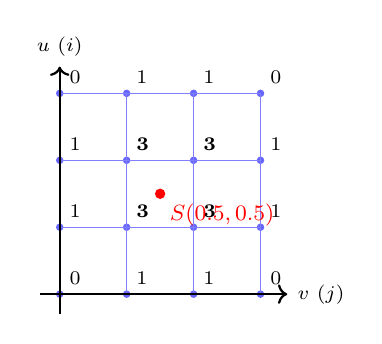
\begin{tikzpicture}[scale=0.85,every node/.style={font=\scriptsize}]
  % grid
  \foreach \i in {0,1,2,3}{
    \foreach \j in {0,1,2,3}{
      \fill[blue!60] (\j,\i) circle (1.6pt);
    }
  }
  % row/col polylines
  \foreach \i in {0,1,2,3}{
    \draw[blue!50,thin] (0,\i)--(1,\i)--(2,\i)--(3,\i);
  }
  \foreach \j in {0,1,2,3}{
    \draw[blue!50,thin] (\j,0)--(\j,1)--(\j,2)--(\j,3);
  }
  % z-labels
  \node[above right] at (0,0) {$0$};
  \node[above right] at (1,0) {$1$};
  \node[above right] at (2,0) {$1$};
  \node[above right] at (3,0) {$0$};
  \node[above right] at (0,1) {$1$};
  \node[above right] at (1,1) {$\mathbf{3}$};
  \node[above right] at (2,1) {$\mathbf{3}$};
  \node[above right] at (3,1) {$1$};
  \node[above right] at (0,2) {$1$};
  \node[above right] at (1,2) {$\mathbf{3}$};
  \node[above right] at (2,2) {$\mathbf{3}$};
  \node[above right] at (3,2) {$1$};
  \node[above right] at (0,3) {$0$};
  \node[above right] at (1,3) {$1$};
  \node[above right] at (2,3) {$1$};
  \node[above right] at (3,3) {$0$};
  % evaluation point S(0.5,0.5)
  \fill[red] (1.5,1.5) circle (2.2pt);
  \node[red,below right] at (1.5,1.5) {\footnotesize $S(0.5,0.5)$};
  % axes
  \draw[->,thick] (-0.3,0)--(3.4,0) node[right]{$v$ ($j$)};
  \draw[->,thick] (0,-0.3)--(0,3.4) node[above]{$u$ ($i$)};
\end{tikzpicture}
\end{center}
\textit{Top-down view: numbers are $z$-heights of $P_{ij}$. Red dot = projected evaluation point.}

% ---------------------------------------------------------------------
\subsection*{6.6 Exam Tips}

\begin{itemize}[leftmargin=*,nosep]
  \item \textbf{Direction discipline:} write down which axis is $u$ (rows $i$) and which is $v$ (columns $j$) before the first arithmetic step.
  \item \textbf{Row-first is usually faster} on paper: you can reuse symmetry between rows (e.g.\ Row 0 vs Row 3, Row 1 vs Row 2) to skip duplicate work.
  \item \textbf{Always sanity-check with Bernstein.} At $(0.5,0.5)$ the cubic weights are $(1,3,3,1)/8$, so the $4\times4$ weights are $\{1,3,9\}/64$ --- \emph{memorise these}.
  \item Check the corner/edge/interior tally: $4{\cdot}1+8{\cdot}3+4{\cdot}9=64$.
  \item For other $(u,v)$, compute $B_i^3(u)$ and $B_j^3(v)$ separately, then form the outer product.
  \item $S(u,v)$ at the corners equals the corner control points: $S(0,0)=P_{00}$ etc.\ --- handy for instant validation.
\end{itemize}

% =====================================================================
\switchcolumn
% =====================================================================
% VIETNAMESE COLUMN
% =====================================================================
\section*{6.\ Ví dụ tính tay: Mặt Bezier bicubic (4$\times$4) tại $(u,v)=(0.5,0.5)$}

\subsection*{6.1 Thiết lập --- lưới control net 4$\times$4}

Một \textbf{mặt Bezier bicubic} (bậc 3 theo cả $u$ và $v$) cần lưới $4\times 4$ control point $\{P_{ij}\}_{i,j=0}^{3}$. Ta dùng lưới ``đồi/lều'' sau (hàng $i$ chạy theo hướng $u$, cột $j$ chạy theo hướng $v$):
\[
\renewcommand{\arraystretch}{1.1}
\begin{array}{c|cccc}
 & j=0 & j=1 & j=2 & j=3 \\\hline
i{=}0 & (0,0,0) & (1,0,1) & (2,0,1) & (3,0,0) \\
i{=}1 & (0,1,1) & (1,1,3) & (2,1,3) & (3,1,1) \\
i{=}2 & (0,2,1) & (1,2,3) & (2,2,3) & (3,2,1) \\
i{=}3 & (0,3,0) & (1,3,1) & (2,3,1) & (3,3,0)
\end{array}
\]
Toạ độ $(x,y)$ nằm trên lưới số nguyên; chỉ thành phần $z$ thay đổi (tạo dạng yên ngựa/đỉnh đồi ở giữa). Ta cần tính $S(0.5,\,0.5)$.

Công thức mặt:
\[
S(u,v)=\sum_{i=0}^{3}\sum_{j=0}^{3} B_i^3(u)\,B_j^3(v)\,P_{ij}.
\]
Ta sẽ tính $S(0.5,0.5)$ \textbf{theo ba cách} và kiểm tra trùng kết quả.

% ---------------------------------------------------------------------
\subsection*{6.2 Cách 1 --- De Casteljau theo hàng trước}

\textbf{Bước A.} Với mỗi hàng $i$, chạy De Casteljau theo $v$ tại $v=0.5$ trên 4 điểm $P_{i0},P_{i1},P_{i2},P_{i3}$ để được $Q_i$.

\textbf{Hàng 0:} $(0,0,0),(1,0,1),(2,0,1),(3,0,0)$
\begin{align*}
\text{L1: }& \tfrac{1}{2}(P_{00}{+}P_{01})=(0.5,0,0.5)\\
           & \tfrac{1}{2}(P_{01}{+}P_{02})=(1.5,0,1)\\
           & \tfrac{1}{2}(P_{02}{+}P_{03})=(2.5,0,0.5)\\
\text{L2: }& \tfrac{1}{2}((0.5,0,0.5){+}(1.5,0,1))=(1.0,0,0.75)\\
           & \tfrac{1}{2}((1.5,0,1){+}(2.5,0,0.5))=(2.0,0,0.75)\\
\text{L3: }& Q_0=\tfrac{1}{2}((1.0,0,0.75){+}(2.0,0,0.75))\\
           &\phantom{Q_0}=(1.5,\,0,\,0.75)
\end{align*}

\textbf{Hàng 1:} $(0,1,1),(1,1,3),(2,1,3),(3,1,1)$
\begin{align*}
\text{L1: }& (0.5,1,2),\;(1.5,1,3),\;(2.5,1,2)\\
\text{L2: }& (1.0,1,2.5),\;(2.0,1,2.5)\\
\text{L3: }& Q_1=(1.5,\,1,\,2.5)
\end{align*}

\textbf{Hàng 2:} có cùng pattern $z$ với Hàng 1 (chỉ $y$ đổi từ 1 sang 2), nhờ tính bất biến affine của De Casteljau ta có
\[
Q_2=(1.5,\,2,\,2.5).
\]

\textbf{Hàng 3:} có cùng pattern $z$ với Hàng 0, nên
\[
Q_3=(1.5,\,3,\,0.75).
\]

\textbf{Bước B.} Bây giờ chạy De Casteljau theo $u$ tại $u=0.5$ trên $Q_0,Q_1,Q_2,Q_3$:
\begin{align*}
\text{L1: }& \tfrac{1}{2}(Q_0{+}Q_1)=(1.5,\,0.5,\,1.625)\\
           & \tfrac{1}{2}(Q_1{+}Q_2)=(1.5,\,1.5,\,2.5)\\
           & \tfrac{1}{2}(Q_2{+}Q_3)=(1.5,\,2.5,\,1.625)\\
\text{L2: }& \tfrac{1}{2}((1.5,0.5,1.625){+}(1.5,1.5,2.5))\\
           &\quad =(1.5,\,1.0,\,2.0625)\\
           & \tfrac{1}{2}((1.5,1.5,2.5){+}(1.5,2.5,1.625))\\
           &\quad =(1.5,\,2.0,\,2.0625)\\
\text{L3: }& S(0.5,0.5)=\tfrac{1}{2}((1.5,1.0,2.0625){+}(1.5,2.0,2.0625))
\end{align*}
\[
\boxed{\,S(0.5,\,0.5)=(1.5,\;1.5,\;2.0625)\,}
\]

% ---------------------------------------------------------------------
\subsection*{6.3 Cách 2 --- Kiểm tra bằng cột trước}

Đảo thứ tự: De Casteljau theo $u$ trên mỗi cột $j$ tại $u=0.5$ để được $R_j$, rồi De Casteljau theo $v$ trên $R_0,R_1,R_2,R_3$ tại $v=0.5$.

\textbf{Cột 0:} $(0,0,0),(0,1,1),(0,2,1),(0,3,0)$\\
$\Rightarrow R_0=(0,\,1.5,\,0.75)$ ($z$ tính giống Hàng 0).

\textbf{Cột 1:} $(1,0,1),(1,1,3),(1,2,3),(1,3,1)$\\
$\Rightarrow R_1=(1,\,1.5,\,2.5)$.

\textbf{Cột 2:} đối xứng $R_2=(2,\,1.5,\,2.5)$.

\textbf{Cột 3:} đối xứng $R_3=(3,\,1.5,\,0.75)$.

De Casteljau trên $R_0,\dots,R_3$ tại $v=0.5$:
\begin{align*}
\text{L1: }& (0.5,1.5,1.625),\;(1.5,1.5,2.5),\;(2.5,1.5,1.625)\\
\text{L2: }& (1.0,1.5,2.0625),\;(2.0,1.5,2.0625)\\
\text{L3: }& (1.5,\,1.5,\,2.0625)\quad\checkmark
\end{align*}
Cùng kết quả --- cấu trúc tích tensor (tensor product) khiến hai thứ tự giao hoán.

% ---------------------------------------------------------------------
\subsection*{6.4 Cách 3 --- Kiểm tra trực tiếp bằng Bernstein}

Tại $t=0.5$ cơ sở Bernstein bậc 3 là
\[
B_i^3(0.5)=\tfrac{1}{8}\big(1,\,3,\,3,\,1\big),\quad i=0,1,2,3.
\]
Trọng số bicubic $w_{ij}=B_i^3(0.5)\,B_j^3(0.5)$ (đơn vị $1/64$):
\[
[w_{ij}]\cdot 64=
\begin{pmatrix}
1 & 3 & 3 & 1\\
3 & 9 & 9 & 3\\
3 & 9 & 9 & 3\\
1 & 3 & 3 & 1
\end{pmatrix}.
\]
Kiểm tra tổng: $4(1)+8(3)+4(9)=4{+}24{+}36=64$. \checkmark

\textbf{Tính thành phần $z$} (chỗ duy nhất không tầm thường). Ma trận $z$:
\[
[z_{ij}]=\begin{pmatrix}0&1&1&0\\1&3&3&1\\1&3&3&1\\0&1&1&0\end{pmatrix}.
\]
\begin{align*}
64\,z &= \underbrace{1\!\cdot\!0\!\cdot\!4}_{\text{4 góc}} + \underbrace{3\!\cdot\!1\!\cdot\!8}_{\text{8 ô cạnh}} + \underbrace{9\!\cdot\!3\!\cdot\!4}_{\text{4 ô trong}}\\
&= 0 + 24 + 108 = 132,\\
z &= 132/64 = 2.0625.\;\checkmark
\end{align*}

\textbf{Thành phần $x$:} với $x_{ij}=j$, mỗi hàng cho cùng giá trị
\[
\bar{x}_{\text{hàng}}=\tfrac{1\cdot0+3\cdot1+3\cdot2+1\cdot3}{8}=\tfrac{12}{8}=1.5,
\]
nên $x=1.5$.

\textbf{Thành phần $y$:} đối xứng với $y_{ij}=i$ cho $y=1.5$.

Kết quả $(1.5,1.5,2.0625)$ \emph{trùng với De Casteljau.} \checkmark

% ---------------------------------------------------------------------
\subsection*{6.5 Sơ đồ control net}

\begin{center}
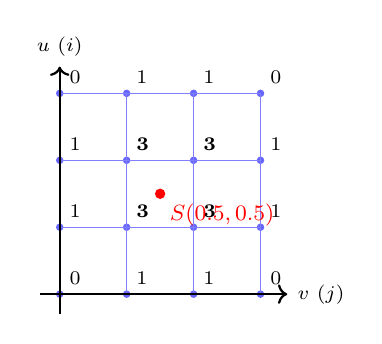
\begin{tikzpicture}[scale=0.85,every node/.style={font=\scriptsize}]
  \foreach \i in {0,1,2,3}{
    \foreach \j in {0,1,2,3}{
      \fill[blue!60] (\j,\i) circle (1.6pt);
    }
  }
  \foreach \i in {0,1,2,3}{
    \draw[blue!50,thin] (0,\i)--(1,\i)--(2,\i)--(3,\i);
  }
  \foreach \j in {0,1,2,3}{
    \draw[blue!50,thin] (\j,0)--(\j,1)--(\j,2)--(\j,3);
  }
  \node[above right] at (0,0) {$0$};
  \node[above right] at (1,0) {$1$};
  \node[above right] at (2,0) {$1$};
  \node[above right] at (3,0) {$0$};
  \node[above right] at (0,1) {$1$};
  \node[above right] at (1,1) {$\mathbf{3}$};
  \node[above right] at (2,1) {$\mathbf{3}$};
  \node[above right] at (3,1) {$1$};
  \node[above right] at (0,2) {$1$};
  \node[above right] at (1,2) {$\mathbf{3}$};
  \node[above right] at (2,2) {$\mathbf{3}$};
  \node[above right] at (3,2) {$1$};
  \node[above right] at (0,3) {$0$};
  \node[above right] at (1,3) {$1$};
  \node[above right] at (2,3) {$1$};
  \node[above right] at (3,3) {$0$};
  \fill[red] (1.5,1.5) circle (2.2pt);
  \node[red,below right] at (1.5,1.5) {\footnotesize $S(0.5,0.5)$};
  \draw[->,thick] (-0.3,0)--(3.4,0) node[right]{$v$ ($j$)};
  \draw[->,thick] (0,-0.3)--(0,3.4) node[above]{$u$ ($i$)};
\end{tikzpicture}
\end{center}
\textit{Nhìn từ trên xuống: số ghi là độ cao $z$ của $P_{ij}$. Chấm đỏ = hình chiếu của điểm cần tính.}

% ---------------------------------------------------------------------
\subsection*{6.6 Mẹo làm bài thi}

\begin{itemize}[leftmargin=*,nosep]
  \item \textbf{Ghi rõ hướng tham số:} viết ngay từ đầu trục nào là $u$ (hàng $i$), trục nào là $v$ (cột $j$) trước khi làm phép tính đầu tiên.
  \item \textbf{Cách hàng-trước (row-first) thường nhanh hơn} khi tính tay: tận dụng đối xứng giữa các hàng (vd.\ Hàng 0 đối xứng Hàng 3, Hàng 1 đối xứng Hàng 2) để bỏ qua phép tính trùng.
  \item \textbf{Luôn check chéo bằng Bernstein.} Tại $(0.5,0.5)$ trọng số bậc 3 là $(1,3,3,1)/8$, nên ma trận $4\times4$ là $\{1,3,9\}/64$ --- \emph{thuộc lòng bộ số này}.
  \item Kiểm tra tổng góc/cạnh/trong: $4{\cdot}1+8{\cdot}3+4{\cdot}9=64$.
  \item Với $(u,v)$ khác, tính $B_i^3(u)$ và $B_j^3(v)$ riêng, rồi nhân ngoài (outer product) thành ma trận $4\times4$.
  \item $S(u,v)$ ở 4 góc bằng đúng 4 control point góc: $S(0,0)=P_{00}$,\dots --- dùng để kiểm tra nhanh.
\end{itemize}

\end{paracol}


\clearpage
\begin{center}
\textbf{\large Part~II — Theoretical Q\&A Bank} \\[1pt]
\footnotesize Essay-style answers organised by topic for quick recall during exam
\end{center}
\vspace{-6pt}\hrule\vspace{4pt}

% =====================================================================
% QA1 - Theoretical Q&A : VR / AR  (bilingual, paracol two-column)
% =====================================================================

\begin{paracol}{2}

\section*{QA1. Theoretical Q\&A --- VR / AR}

\textbf{Q1. What is Virtual Reality (VR)?}\\
\textbf{Virtual Reality} is a computer-generated, fully \textbf{immersive} 3D environment that completely replaces the user's real-world view. The user wears a \textbf{Head-Mounted Display (HMD)} such as the \textbf{Meta Quest 3}, \textbf{HTC Vive Pro}, \textbf{Valve Index}, or \textbf{PlayStation VR2}, plus tracked controllers and sometimes haptic gloves. The system tracks the user's head and hand pose in real time and renders a \textbf{stereoscopic} pair of images (one per eye) at \textbf{90--120 Hz} so the brain perceives true depth. The goals of VR are \textbf{presence} (the feeling of ``being there'') and \textbf{immersion} (sensory replacement). Typical applications include training simulators, surgical rehearsal, exposure therapy, architectural walkthroughs, and games such as \textit{Half-Life: Alyx} and \textit{Beat Saber}.

\switchcolumn

\section*{QA1. Câu hỏi lý thuyết --- VR / AR}

\textbf{Câu 1. Thực tại ảo (VR) là gì?}\\
\textbf{Virtual Reality (VR)} là một môi trường 3D do máy tính tạo ra, \textbf{hoàn toàn thay thế} thế giới thực mà người dùng nhìn thấy. Người dùng đeo một \textbf{Head-Mounted Display (HMD)} như \textbf{Meta Quest 3}, \textbf{HTC Vive Pro}, \textbf{Valve Index} hoặc \textbf{PSVR2}, kèm theo controller và đôi khi haptic gloves. Hệ thống \textbf{tracking} đầu và tay người dùng theo thời gian thực, rồi \textbf{render} một cặp ảnh \textbf{stereoscopic} (mỗi mắt một ảnh) ở \textbf{90--120 Hz} để não cảm nhận chiều sâu. Mục tiêu của VR là tạo \textbf{presence} (cảm giác ``đang ở trong đó'') và \textbf{immersion} (thay thế cảm giác). Ứng dụng phổ biến: huấn luyện, mô phỏng phẫu thuật, trị liệu phơi nhiễm, đi dạo kiến trúc, game như \textit{Half-Life: Alyx}, \textit{Beat Saber}.

\switchcolumn*

\textbf{Q2. What is Augmented Reality (AR)?}\\
\textbf{Augmented Reality} \textit{augments} the real world by overlaying digital content (3D models, text, animations) onto the user's view of the physical environment, instead of replacing it. AR can run on \textbf{smartphones/tablets} (video see-through, e.g.\ Pokemon Go, IKEA Place) or on \textbf{AR glasses} (optical see-through, e.g.\ Microsoft HoloLens 2, Magic Leap 2, Apple Vision Pro in passthrough). Core capabilities are \textbf{6DoF tracking}, \textbf{plane detection}, \textbf{anchoring}, \textbf{occlusion}, and \textbf{light estimation}. Common SDKs are \textbf{ARKit} (iOS), \textbf{ARCore} (Android), \textbf{Vuforia} (cross-platform marker-based), and \textbf{Unity AR Foundation} (unifies them). Applications include navigation arrows on streets, surgical guidance overlay, AR try-on for retail, and industrial maintenance instructions.

\switchcolumn

\textbf{Câu 2. Thực tại tăng cường (AR) là gì?}\\
\textbf{Augmented Reality (AR)} \textit{bổ sung} nội dung số (mô hình 3D, text, animation) lên thế giới thực thay vì thay thế nó. AR chạy trên \textbf{smartphone/tablet} (video see-through, ví dụ Pokemon Go, IKEA Place) hoặc trên \textbf{AR glasses} (optical see-through như HoloLens 2, Magic Leap 2, Apple Vision Pro). Năng lực cốt lõi gồm: \textbf{6DoF tracking}, \textbf{plane detection}, \textbf{anchoring}, \textbf{occlusion}, \textbf{light estimation}. Các SDK phổ biến: \textbf{ARKit} (iOS), \textbf{ARCore} (Android), \textbf{Vuforia} (cross-platform, marker-based), \textbf{Unity AR Foundation} (gói chung). Ứng dụng: chỉ đường ngoài phố, hướng dẫn phẫu thuật, thử đồ ảo, hướng dẫn bảo trì công nghiệp.

\switchcolumn*

\textbf{Q3. What is Mixed Reality (MR)?}\\
\textbf{Mixed Reality} sits between AR and VR on the \textbf{Milgram Reality--Virtuality Continuum}. In MR, virtual objects are not just overlaid but actually \textbf{interact with} the real environment: they understand the geometry of walls and furniture, support \textbf{occlusion} (a real hand can hide a virtual ball), respond to real lighting, and accept physical interaction. MR therefore requires \textbf{spatial mapping} (a real-time mesh of the room produced by depth sensors) plus \textbf{hand and eye tracking}. Devices designed for MR include the \textbf{Microsoft HoloLens 2}, \textbf{Magic Leap 2}, \textbf{Meta Quest 3} (color passthrough), and \textbf{Apple Vision Pro}. Use cases: collaborative engineering review, holographic medical training, factory digital twins.

\switchcolumn

\textbf{Câu 3. Mixed Reality (MR) là gì?}\\
\textbf{Mixed Reality (MR)} nằm giữa AR và VR trên \textbf{Milgram Reality--Virtuality Continuum}. Vật thể ảo không chỉ ``đè lên'' mà thực sự \textbf{tương tác} với môi trường thật: hiểu được hình học tường, bàn ghế, hỗ trợ \textbf{occlusion} (tay thật che được quả bóng ảo), phản ứng với ánh sáng thật, và cho phép tương tác vật lý. MR vì vậy cần \textbf{spatial mapping} (lưới 3D của phòng từ depth sensor) cộng với \textbf{hand tracking} và \textbf{eye tracking}. Thiết bị MR: \textbf{HoloLens 2}, \textbf{Magic Leap 2}, \textbf{Meta Quest 3} (color passthrough), \textbf{Apple Vision Pro}. Use case: review kỹ thuật phối hợp, huấn luyện y khoa hologram, digital twin nhà máy.

\switchcolumn*

\textbf{Q4. What is XR (Extended Reality)?}\\
\textbf{XR} is the \textbf{umbrella term} that encompasses VR, AR, and MR --- ``X'' stands for any reality. It is used in industry standards (e.g., \textbf{OpenXR}) and in research because the boundaries between the three are increasingly blurry: a Quest~3 in passthrough mode is AR/MR, the same device with passthrough off is VR. Talking about ``XR'' lets us describe \textbf{cross-cutting concerns} such as tracking, rendering, input, ergonomics, and content authoring without committing to one mode. The \textbf{OpenXR} standard (Khronos Group) is the de-facto cross-vendor API, supported by Meta, Microsoft, Valve, HTC, Pico, and Apple. Modern game engines like \textbf{Unity} and \textbf{Unreal} target OpenXR so a single codebase runs on all major XR headsets.

\switchcolumn

\textbf{Câu 4. XR (Extended Reality) là gì?}\\
\textbf{XR} là \textbf{thuật ngữ ô} bao gồm VR, AR và MR --- ``X'' nghĩa là bất kỳ loại reality nào. Nó được dùng trong chuẩn công nghiệp (ví dụ \textbf{OpenXR}) và trong nghiên cứu, vì ranh giới giữa ba loại ngày càng mờ: Quest 3 bật passthrough là AR/MR, tắt passthrough thì là VR. Dùng từ ``XR'' giúp ta nói về các vấn đề \textbf{xuyên suốt} như tracking, render, input, ergonomic mà không cần chọn loại cụ thể. Chuẩn \textbf{OpenXR} (Khronos Group) là API cross-vendor de-facto, hỗ trợ bởi Meta, Microsoft, Valve, HTC, Pico, Apple. Các engine \textbf{Unity}, \textbf{Unreal} đều target OpenXR nên một codebase chạy được trên đa số headset.

\switchcolumn*

\textbf{Q5. Compare VR vs AR vs MR (in one paragraph and a table).}\\
The three differ mainly in \textbf{how much real world remains visible} and \textbf{how virtual objects interact with reality}.\\
\begin{tabular}{@{}lccc@{}}
\toprule
 & VR & AR & MR\\
\midrule
Real world & hidden & visible & visible\\
Virtual obj.\ & full env. & overlay & integrated\\
Interaction & with virt. & passive & with real\\
Display & opaque HMD & phone/glass & MR HMD\\
Example & Quest VR & Pokemon Go & HoloLens 2\\
\bottomrule
\end{tabular}\\
In short: \textbf{VR replaces}, \textbf{AR adds on top}, \textbf{MR blends with awareness}. All three sit on the Milgram continuum and are unified under \textbf{XR}.

\switchcolumn

\textbf{Câu 5. So sánh VR, AR, MR (1 đoạn + bảng).}\\
Khác biệt chính nằm ở \textbf{lượng thế giới thực còn nhìn thấy} và \textbf{mức độ tương tác} của vật thể ảo với thực tại.\\
\begin{tabular}{@{}lccc@{}}
\toprule
 & VR & AR & MR\\
\midrule
TG thực & ẩn & thấy & thấy\\
Vật ảo & toàn bộ & overlay & tích hợp\\
Tương tác & với ảo & thụ động & với thực\\
Display & HMD đen & phone/kính & MR HMD\\
Ví dụ & Quest VR & Pokemon Go & HoloLens 2\\
\bottomrule
\end{tabular}\\
Tóm lại: \textbf{VR thay thế}, \textbf{AR thêm vào}, \textbf{MR hòa quyện}. Cả ba nằm trên Milgram continuum và gộp chung thành \textbf{XR}.

\switchcolumn*

\textbf{Q6. What is an HMD and what are its main components?}\\
A \textbf{Head-Mounted Display (HMD)} is the wearable display that puts visuals close to the eyes. Its main components are: (1) two \textbf{micro-displays} (LCD, OLED, or micro-OLED), one per eye, with resolutions like $2064\times2208$ per eye on Quest 3; (2) \textbf{Fresnel} or \textbf{pancake lenses} that magnify the image so the eye can focus at near distance; (3) an \textbf{IPD adjustment} for inter-pupillary distance; (4) an \textbf{IMU} (gyroscope + accelerometer + magnetometer) for fast head rotation tracking; (5) outward-facing \textbf{cameras} for inside-out 6DoF tracking and passthrough; (6) sometimes \textbf{eye-tracking cameras} for foveated rendering. Standalone HMDs (Quest 3) include an SoC like Snapdragon XR2~Gen~2; PC-VR HMDs (Vive Pro 2, Index) stream from a GPU through DisplayPort.

\switchcolumn

\textbf{Câu 6. HMD là gì? Các thành phần chính.}\\
\textbf{Head-Mounted Display (HMD)} là thiết bị đeo đầu đưa hình ảnh sát mắt. Thành phần chính: (1) hai \textbf{micro-display} (LCD, OLED hoặc micro-OLED), mỗi mắt một, ví dụ Quest 3 có $2064\times2208$ mỗi mắt; (2) \textbf{Fresnel} hoặc \textbf{pancake lens} phóng đại để mắt focus được ở khoảng gần; (3) \textbf{IPD adjustment} để chỉnh khoảng cách hai mắt; (4) \textbf{IMU} (gyro + accel + magnetometer) đo xoay đầu siêu nhanh; (5) \textbf{camera} hướng ngoài để inside-out 6DoF tracking và passthrough; (6) đôi khi có \textbf{eye-tracking camera} cho foveated rendering. HMD standalone (Quest 3) có SoC kiểu Snapdragon XR2 Gen 2; PC-VR HMD (Vive Pro 2, Index) nhận stream từ GPU qua DisplayPort.

\switchcolumn*

\textbf{Q7. What is 6DoF tracking? Compare with 3DoF.}\\
\textbf{Degrees of Freedom (DoF)} = number of independent motions the system can sense. \textbf{3DoF} senses only \textit{rotations} around three axes (yaw, pitch, roll) --- the user can look around but cannot walk; typical of cheap mobile VR like the original Cardboard or Oculus Go. \textbf{6DoF} adds the three \textit{translations} (forward/back, left/right, up/down), so the user can physically walk around and lean. 6DoF requires either \textbf{outside-in} tracking (e.g., HTC Vive Lighthouse base stations emitting IR sweeps) or \textbf{inside-out} tracking (cameras on the HMD doing visual SLAM, e.g., Quest 3, HoloLens 2). 6DoF is essential for \textbf{presence}, room-scale interaction, and is the standard for any modern VR/AR experience.

\switchcolumn

\textbf{Câu 7. 6DoF tracking là gì? So với 3DoF?}\\
\textbf{Degrees of Freedom (DoF)} = số chuyển động độc lập hệ thống cảm nhận được. \textbf{3DoF} chỉ cảm nhận \textit{xoay} quanh 3 trục (yaw/pitch/roll) --- người dùng nhìn quanh được nhưng không đi được; đặc trưng của mobile VR rẻ như Cardboard hoặc Oculus Go. \textbf{6DoF} thêm 3 chiều \textit{tịnh tiến} (trước/sau, trái/phải, lên/xuống), người dùng đi và nghiêng được. 6DoF cần \textbf{outside-in} (HTC Vive Lighthouse phát IR sweep) hoặc \textbf{inside-out} (camera trên HMD chạy visual SLAM, ví dụ Quest 3, HoloLens 2). 6DoF là điều kiện cần để có \textbf{presence}, room-scale interaction, và là chuẩn của VR/AR hiện đại.

\switchcolumn*

\textbf{Q8. What is SLAM and how does it work?}\\
\textbf{SLAM = Simultaneous Localization And Mapping}. The headset (or robot, drone, phone) builds a map of an unknown environment \textit{while} tracking its own pose inside that map, in real time. Pipeline: (1) \textbf{Feature extraction} from each frame (corners/keypoints via FAST, ORB, or learned features); (2) \textbf{Feature matching} between consecutive frames; (3) \textbf{Pose estimation} via PnP / essential matrix; (4) \textbf{IMU fusion} with an Extended Kalman Filter or factor graph for smoothness during fast motion; (5) \textbf{Mapping}: triangulate matched features into 3D landmarks; (6) \textbf{Loop closure} corrects accumulated \textbf{drift} when a previously seen place is recognized; (7) \textbf{Bundle adjustment} optimizes all poses + landmarks. Visual--inertial SLAM (VI-SLAM) underlies ARKit, ARCore, HoloLens, and Quest tracking.

\switchcolumn

\textbf{Câu 8. SLAM là gì? Hoạt động ra sao?}\\
\textbf{SLAM = Simultaneous Localization And Mapping}. Headset (hoặc robot, drone, phone) vừa \textit{xây bản đồ} môi trường lạ, vừa \textit{định vị bản thân} trong bản đồ đó, theo thời gian thực. Pipeline: (1) \textbf{Feature extraction} từ mỗi frame (góc/keypoint qua FAST, ORB hoặc deep features); (2) \textbf{Feature matching} giữa các frame liên tiếp; (3) \textbf{Pose estimation} qua PnP / essential matrix; (4) \textbf{IMU fusion} bằng Extended Kalman Filter hoặc factor graph cho mượt khi chuyển động nhanh; (5) \textbf{Mapping}: tam giác hóa các feature thành landmark 3D; (6) \textbf{Loop closure} sửa \textbf{drift} khi nhận ra nơi cũ; (7) \textbf{Bundle adjustment} tối ưu toàn bộ pose + landmark. Visual--inertial SLAM (VI-SLAM) là nền của ARKit, ARCore, HoloLens, Quest.

\switchcolumn*

\textbf{Q9. What is presence? What is immersion?}\\
\textbf{Immersion} is an \textbf{objective property of the system}: how well the hardware replaces sensory input (high resolution, wide \textbf{FOV}, low latency, spatial audio, haptics). \textbf{Presence} is the \textbf{subjective feeling} of ``being there'' that the user experiences \textit{because} immersion is high. Immersion enables presence but does not guarantee it: bad content, low frame rate, or cybersickness can break presence even on great hardware. Presence is usually measured with \textbf{questionnaires} like the Slater--Usoh--Steed (SUS) or Witmer--Singer Presence Questionnaire, or with physiological proxies (heart rate, EDA). Designers maximize presence with consistent \textbf{6DoF tracking}, $\geq$~90~Hz refresh, $<$~20~ms motion-to-photon latency, spatial audio, and believable interaction.

\switchcolumn

\textbf{Câu 9. Presence là gì? Immersion là gì?}\\
\textbf{Immersion} là \textbf{thuộc tính khách quan của hệ thống}: phần cứng thay thế giác quan tốt đến đâu (độ phân giải cao, \textbf{FOV} rộng, latency thấp, âm thanh không gian, haptic). \textbf{Presence} là \textbf{cảm giác chủ quan} ``đang ở đó'' mà người dùng cảm thấy \textit{nhờ} immersion cao. Immersion là điều kiện cần nhưng chưa đủ: nội dung dở, FPS thấp, cybersickness đều có thể phá vỡ presence. Presence thường đo bằng \textbf{questionnaire} như Slater--Usoh--Steed (SUS), Witmer--Singer, hoặc đo sinh lý (nhịp tim, EDA). Thiết kế tốt để tối đa presence: \textbf{6DoF tracking} ổn định, $\geq$~90~Hz, motion-to-photon $<$~20~ms, spatial audio, tương tác thuyết phục.

\switchcolumn*

\textbf{Q10. How does VR work step-by-step (the rendering loop)?}\\
The VR loop runs at 90--120~Hz and must finish each frame in $\sim$11~ms or less:\\
\textbf{(1) Sense:} read \textbf{IMU} + cameras to update head pose; \textbf{(2) Predict:} extrapolate the pose to the photon-display time (\textbf{motion prediction}); \textbf{(3) Update:} run game logic, physics, animation; \textbf{(4) Cull:} frustum + occlusion culling; \textbf{(5) Render twice:} produce the \textit{left-eye} and \textit{right-eye} images using two slightly offset projection matrices (one per camera, separated by IPD); \textbf{(6) Distortion correction:} pre-warp each image to cancel the lens's pincushion distortion and chromatic aberration; \textbf{(7) Asynchronous Time Warp / Space Warp:} just before scan-out, re-project the finished image with the latest pose to compensate for any remaining latency; \textbf{(8) Scan out} to the panel, scanline-synced. Spatial audio is computed in parallel with HRTFs.

\switchcolumn

\textbf{Câu 10. VR hoạt động từng bước thế nào (rendering loop)?}\\
Vòng VR chạy 90--120~Hz, mỗi frame phải xong trong $\sim$11~ms:\\
\textbf{(1) Sense:} đọc \textbf{IMU} + camera, cập nhật head pose; \textbf{(2) Predict:} ngoại suy pose tới thời điểm photon ra màn (\textbf{motion prediction}); \textbf{(3) Update:} game logic, physics, animation; \textbf{(4) Cull:} frustum + occlusion culling; \textbf{(5) Render hai lần:} ảnh \textit{mắt trái} và \textit{mắt phải} với hai ma trận chiếu lệch nhau (cách nhau IPD); \textbf{(6) Distortion correction:} pre-warp để khử pincushion và chromatic aberration của thấu kính; \textbf{(7) Asynchronous Time Warp / Space Warp:} ngay trước scan-out, re-project ảnh đã render bằng pose mới nhất để bù latency; \textbf{(8) Scan out} ra panel theo scanline. Spatial audio tính song song bằng HRTF.

\switchcolumn*

\textbf{Q11. How does the AR pipeline work step-by-step?}\\
\textbf{(1) Camera capture:} grab the next frame from the rear camera (or passthrough cameras); \textbf{(2) Tracking:} run \textbf{VI-SLAM} to estimate the device's 6DoF pose; \textbf{(3) Scene understanding:} detect \textbf{planes} (floor, table), feature points, meshes, faces, hands, image targets; \textbf{(4) Light estimation:} infer ambient intensity, color, and a directional source (or spherical harmonics) from the camera image; \textbf{(5) Anchor management:} attach virtual objects to anchors that are stable in the real world; \textbf{(6) Rendering:} render virtual objects with the camera's intrinsics and the estimated pose; apply real-world lighting; perform \textbf{occlusion} using the depth map or scene mesh; \textbf{(7) Composite:} blend the rendered overlay with the camera image (video see-through) or display on the optical combiner (optical see-through); \textbf{(8) Display} at $\geq$~60~Hz.

\switchcolumn

\textbf{Câu 11. AR pipeline hoạt động từng bước?}\\
\textbf{(1) Camera capture:} lấy frame mới từ camera sau (hoặc camera passthrough); \textbf{(2) Tracking:} chạy \textbf{VI-SLAM} để ước lượng 6DoF pose của thiết bị; \textbf{(3) Scene understanding:} dò \textbf{plane} (sàn, bàn), feature point, mesh, mặt người, tay, image target; \textbf{(4) Light estimation:} suy ra cường độ, màu sắc môi trường + nguồn sáng định hướng (hoặc spherical harmonics) từ ảnh camera; \textbf{(5) Anchor management:} gắn vật ảo vào anchor cố định trong không gian thật; \textbf{(6) Rendering:} render vật ảo theo intrinsic của camera và pose ước lượng; áp ánh sáng thực; thực hiện \textbf{occlusion} dùng depth map hoặc scene mesh; \textbf{(7) Composite:} blend overlay với ảnh camera (video see-through) hoặc hiển thị qua combiner quang (optical see-through); \textbf{(8) Hiển thị} ở $\geq$~60~Hz.

\switchcolumn*

\textbf{Q12. How does inside-out tracking work?}\\
In \textbf{inside-out tracking}, the cameras are \textit{on the headset} and look outward; there are no external base stations. Each frame, the system extracts \textbf{visual features} (corners), matches them across multiple cameras (stereo or wider arrays) and across time, and combines this with the \textbf{IMU} via \textbf{visual--inertial odometry}. The result is a 6DoF pose at very high rate (1000~Hz from IMU, corrected by 30--60~Hz visual updates). For controllers, the same outward cameras observe \textbf{IR LEDs} on the controller (Quest's constellation) or perform fully optical hand tracking (HoloLens, Quest hand tracking, Vision Pro). Pros: no setup, portable, fewer cables. Cons: needs textured environment, can lose tracking in the dark or in front of a blank wall, controller can be lost behind the back.

\switchcolumn

\textbf{Câu 12. Inside-out tracking hoạt động ra sao?}\\
Trong \textbf{inside-out tracking}, camera nằm \textit{trên headset}, hướng ra ngoài; không cần base station. Mỗi frame, hệ thống trích \textbf{feature} (góc), match qua nhiều camera (stereo hoặc nhiều hơn) và qua thời gian, kết hợp với \textbf{IMU} bằng \textbf{visual--inertial odometry}. Kết quả là 6DoF pose tần số rất cao (IMU 1000 Hz, hiệu chỉnh bằng visual 30--60 Hz). Với controller: cùng camera đó quan sát \textbf{IR LED} trên tay cầm (Quest constellation) hoặc làm hand tracking thuần optical (HoloLens, Quest hand tracking, Vision Pro). Ưu: không cần setup, di động, ít cáp. Nhược: cần môi trường có texture, mất tracking trong tối hoặc trước tường trắng, controller có thể mất khi giấu sau lưng.

\switchcolumn*

\textbf{Q13. Compare outside-in (Lighthouse) vs inside-out tracking.}\\
\textbf{Outside-in} uses external sensors (Lighthouse base stations sweeping IR planes; or external cameras like the original Oculus Rift CV1) that observe the headset/controllers; \textbf{inside-out} reverses this: cameras are on the headset. Outside-in offers \textbf{sub-millimeter precision}, near-zero jitter, large play areas (Vive Lighthouse covers $\sim$10~m), and reliable controller tracking even behind the back. Its drawbacks: cumbersome setup, fixed play space, needs power outlets and line-of-sight. Inside-out is \textbf{plug-and-play}, portable, cheaper, supports any room, but has slightly more jitter, can drift, struggles in low light or feature-poor rooms, and may lose controllers occluded from the headset cameras. Modern consumer HMDs (Quest, HoloLens, Vision Pro, PSVR2) all use inside-out; pro/research setups still favor Lighthouse.

\switchcolumn

\textbf{Câu 13. So sánh outside-in (Lighthouse) vs inside-out.}\\
\textbf{Outside-in} dùng cảm biến ngoài (Lighthouse phát mặt phẳng IR; hoặc camera ngoài như Rift CV1) quan sát headset/controller; \textbf{inside-out} ngược lại, camera nằm trên headset. Outside-in cho \textbf{độ chính xác sub-mm}, gần như không jitter, vùng chơi rộng (Vive Lighthouse phủ $\sim$10~m), tracking controller ổn định kể cả sau lưng. Nhược: setup phức tạp, vùng chơi cố định, cần ổ cắm và line-of-sight. Inside-out là \textbf{plug-and-play}, di động, rẻ, hỗ trợ mọi phòng, nhưng jitter hơn, có drift, kém trong tối hoặc phòng ít texture, mất controller khi bị che. HMD tiêu dùng hiện nay (Quest, HoloLens, Vision Pro, PSVR2) dùng inside-out; setup chuyên nghiệp/nghiên cứu vẫn ưa Lighthouse.

\switchcolumn*

\textbf{Q14. How does marker-based AR work?}\\
\textbf{Marker-based AR} relies on a known image (\textbf{fiducial marker} like ARTag/ArUco, or a textured \textbf{image target} in Vuforia) printed in the real world. Steps: (1) The camera grabs a frame; (2) The image is binarized/thresholded and contours are found; (3) Quadrilateral contours are matched against the marker's known pattern (or feature descriptors are matched against the image database); (4) The four corners give a 2D--3D correspondence; (5) Solving \textbf{PnP (Perspective-n-Point)} with the camera intrinsics yields the 6DoF pose of the marker relative to the camera; (6) A virtual object is rendered at that pose. Marker-based AR is \textbf{robust, fast, and free of drift}, used in print-to-AR books, museum exhibits, packaging promotions, and education --- but the marker must remain visible.

\switchcolumn

\textbf{Câu 14. Marker-based AR hoạt động thế nào?}\\
\textbf{Marker-based AR} dựa vào ảnh đã biết (\textbf{fiducial marker} kiểu ARTag/ArUco, hoặc \textbf{image target} có texture trong Vuforia) đặt trong thế giới thực. Bước: (1) Camera lấy frame; (2) Ảnh được binarize/threshold, tìm contour; (3) Contour tứ giác được match với pattern marker (hoặc feature descriptor match với database); (4) Bốn góc cho tương ứng 2D--3D; (5) Giải \textbf{PnP (Perspective-n-Point)} với intrinsic camera $\Rightarrow$ 6DoF pose của marker so với camera; (6) Render vật ảo tại pose đó. Marker-based AR \textbf{ổn định, nhanh, không drift}, dùng trong sách AR, bảo tàng, bao bì khuyến mại, giáo dục --- nhưng marker phải luôn nhìn thấy.

\switchcolumn*

\textbf{Q15. Compare marker-based vs markerless AR.}\\
\textbf{Marker-based} requires a printed marker/image target in the scene; \textbf{markerless} relies on natural features and SLAM. Marker-based is \textbf{simple, robust, drift-free, low-cost} but constrained: the experience dies if the marker is occluded, lit poorly, or out of frame. Markerless (ARKit, ARCore, HoloLens) discovers planes and feature points anywhere, supports walking around the scene, and enables persistent \textbf{world anchors} via cloud anchoring (ARCore Cloud Anchors, ARKit ARWorldMap). Its trade-offs are higher compute, dependence on texture and lighting, and \textbf{drift} that needs loop closure. Practical rule: use marker-based for short, controlled experiences (museum cards, packaging, education); use markerless for room-scale, navigation, and large-area AR.

\switchcolumn

\textbf{Câu 15. So sánh marker-based vs markerless AR.}\\
\textbf{Marker-based} cần marker/image target in sẵn; \textbf{markerless} dựa vào feature tự nhiên + SLAM. Marker-based \textbf{đơn giản, ổn, không drift, rẻ} nhưng bị ràng buộc: marker bị che, thiếu sáng, ngoài khung là ``chết''. Markerless (ARKit, ARCore, HoloLens) phát hiện plane và feature mọi nơi, đi lại được, hỗ trợ \textbf{world anchor} bền qua cloud (ARCore Cloud Anchors, ARKit ARWorldMap). Nhược điểm: tốn compute, phụ thuộc texture và ánh sáng, có \textbf{drift} cần loop closure. Quy tắc thực tế: marker-based cho trải nghiệm ngắn, có kiểm soát (bảo tàng, bao bì, giáo dục); markerless cho room-scale, dẫn đường, AR diện rộng.

\switchcolumn*

\textbf{Q16. Compare optical see-through vs video see-through.}\\
\textbf{Optical see-through (OST)}: light from the real world reaches the eye through a transparent \textbf{combiner} (waveguide, beam-splitter); virtual content is projected onto it. Used by HoloLens 2, Magic Leap 2, smart glasses. Pros: \textbf{zero camera latency} for the real view, natural depth, safer (you actually see). Cons: limited \textbf{FOV} ($\sim$50$^\circ$ on HL2), virtual objects look semi-transparent, hard to render true black, expensive optics. \textbf{Video see-through (VST)}: outward cameras capture the world, the system composites virtuals on top, and the result is shown on opaque displays (Quest 3, Vision Pro, Varjo XR-4). Pros: \textbf{wide FOV}, perfect occlusion, dynamic range, full opacity for virtuals. Cons: camera latency, distortion, lower fidelity than direct vision, total visual blackout if the system crashes.

\switchcolumn

\textbf{Câu 16. So sánh optical vs video see-through.}\\
\textbf{Optical see-through (OST)}: ánh sáng thực đi qua \textbf{combiner} trong suốt (waveguide, beam-splitter); nội dung ảo được chiếu lên đó. HoloLens 2, Magic Leap 2, smart glasses dùng cách này. Ưu: \textbf{0 ms camera latency} cho cảnh thực, depth tự nhiên, an toàn hơn. Nhược: \textbf{FOV} hẹp ($\sim$50$^\circ$ ở HL2), vật ảo trong mờ, khó render màu đen thật, optics đắt. \textbf{Video see-through (VST)}: camera ngoài quay cảnh thực, ghép ảo lên, hiển thị qua màn hình kín (Quest 3, Vision Pro, Varjo XR-4). Ưu: \textbf{FOV rộng}, occlusion hoàn hảo, dải động cao, ảo phủ kín được. Nhược: latency camera, distortion, độ trung thực kém mắt thường, mất hình toàn bộ nếu hệ thống crash.

\switchcolumn*

\textbf{Q17. How does stereoscopic rendering produce depth?}\\
The brain extracts depth from many cues; the strongest near-field cue is \textbf{binocular disparity} --- the slight horizontal offset between the images received by the left and right eye. To replicate this, a VR engine maintains \textbf{two virtual cameras} separated by the user's \textbf{IPD} ($\sim$63~mm) and renders each frame twice with slightly different view matrices but the same model and projection setup (with appropriate eye offsets). Each rendered image is sent to its eye's panel through the lens. The brain fuses the two images and infers depth. Additional cues are \textbf{motion parallax} (provided by 6DoF head tracking) and \textbf{vergence}. Mismatch between vergence and the fixed lens focus causes the \textbf{vergence--accommodation conflict (VAC)}, a known cause of fatigue and a target of varifocal R\&D.

\switchcolumn

\textbf{Câu 17. Stereoscopic render tạo depth thế nào?}\\
Não suy ra depth từ nhiều cue; cue gần mạnh nhất là \textbf{binocular disparity} --- chênh lệch ngang giữa ảnh hai mắt. Để mô phỏng, engine VR đặt \textbf{hai camera ảo} cách nhau bằng \textbf{IPD} ($\sim$63~mm), mỗi frame render hai lần với view matrix lệch (chung model + projection có offset mắt). Mỗi ảnh đi qua thấu kính tới panel của mắt tương ứng. Não fuse hai ảnh và tính ra depth. Cue phụ: \textbf{motion parallax} (do 6DoF head tracking cung cấp) và \textbf{vergence}. Khi vergence lệch tiêu cự cố định của thấu kính sẽ gây \textbf{vergence--accommodation conflict (VAC)} --- nguyên nhân mỏi mắt, đang là chủ đề R\&D varifocal.

\switchcolumn*

\textbf{Q18. How does foveated rendering work and why use it?}\\
The human retina has high resolution only in the \textbf{fovea} ($\sim$5$^\circ$ at the center of gaze); peripheral vision is much lower resolution. \textbf{Foveated rendering} exploits this by rendering the \textbf{gaze-centered region at full resolution} and the periphery at progressively lower resolution, then blending. \textbf{Eye-tracked} variant (PSVR2, Vision Pro, Quest Pro) uses real-time gaze; \textbf{fixed} variant (Quest 2/3 default) just lowers resolution at panel edges. Benefits: \textbf{30--70\% GPU savings}, enabling higher-fidelity scenes or lower power on standalone HMDs. Implementation in graphics APIs: \textbf{Variable Rate Shading (VRS)}, Vulkan VK\_EXT\_fragment\_density\_map, NVIDIA VRSS. The technique is essential for high-resolution headsets ($>$~3K per eye) where full-res rendering would not fit a 90~Hz budget.

\switchcolumn

\textbf{Câu 18. Foveated rendering hoạt động thế nào, vì sao dùng?}\\
Võng mạc người chỉ có độ phân giải cao ở \textbf{fovea} ($\sim$5$^\circ$ trung tâm); vùng ngoại vi thấp hơn nhiều. \textbf{Foveated rendering} tận dụng điều đó: render \textbf{vùng nhìn} ở full resolution, vùng ngoại vi giảm dần resolution rồi blend. Bản \textbf{eye-tracked} (PSVR2, Vision Pro, Quest Pro) dùng gaze thực; bản \textbf{fixed} (Quest 2/3 mặc định) chỉ giảm resolution ở rìa panel. Lợi ích: \textbf{tiết kiệm GPU 30--70\%}, cho phép scene đẹp hơn hoặc tiết kiệm pin trên HMD standalone. Triển khai bằng \textbf{Variable Rate Shading (VRS)}, Vulkan VK\_EXT\_fragment\_density\_map, NVIDIA VRSS. Kỹ thuật này gần như bắt buộc với headset $>$~3K mỗi mắt vì render full-res không kịp 90~Hz.

\switchcolumn*

\textbf{Q19. Why is low latency critical in VR? What is motion-to-photon?}\\
\textbf{Motion-to-photon (M2P) latency} is the total time from a real head movement until the corresponding photon hits the eye. If M2P is too high, the image lags the head, the brain detects a mismatch between vestibular and visual systems, and \textbf{cybersickness} results. Research and industry consensus: \textbf{M2P should be under 20~ms}; great systems achieve \textbf{$<$~15~ms}. Latency is reduced by: (1) high-frequency IMU + prediction; (2) pipelined GPU rendering; (3) \textbf{Asynchronous Time Warp (ATW)} re-projects the last rendered frame using fresh head pose right before scan-out; (4) \textbf{Asynchronous Space Warp (ASW)} synthesizes intermediate frames; (5) racing-the-beam scan-out. High refresh rate (90/120/144~Hz) further reduces effective latency and judder.

\switchcolumn

\textbf{Câu 19. Vì sao latency thấp quan trọng trong VR? Motion-to-photon là gì?}\\
\textbf{Motion-to-photon (M2P) latency} là tổng thời gian từ khi đầu chuyển động thực tới khi photon tới mắt. Nếu M2P cao, ảnh trễ so với đầu, não phát hiện lệch giữa tiền đình và thị giác $\Rightarrow$ \textbf{cybersickness}. Đồng thuận: \textbf{M2P dưới 20~ms}; hệ tốt đạt \textbf{$<$~15~ms}. Cách giảm latency: (1) IMU tần số cao + prediction; (2) GPU render pipelined; (3) \textbf{Asynchronous Time Warp (ATW)} re-project frame cũ bằng pose mới trước khi scan-out; (4) \textbf{Asynchronous Space Warp (ASW)} sinh frame trung gian; (5) racing-the-beam scan-out. Refresh rate cao (90/120/144~Hz) giảm thêm latency hữu hiệu và judder.

\switchcolumn*

\textbf{Q20. Why does motion sickness (cybersickness) occur in VR? How to prevent it?}\\
\textbf{Cybersickness} arises mainly from a \textbf{sensory conflict} between the visual system (which says ``I'm moving'') and the \textbf{vestibular system} (which says ``I'm sitting still''). Triggers: high latency, low frame rate, artificial \textbf{smooth locomotion}, vection, narrow FOV vignetting absent, miscalibrated IPD, lens distortion errors. Mitigation: \textbf{(1)} keep M2P $<$~20~ms and frame rate $\geq$~90~Hz; \textbf{(2)} use \textbf{teleport locomotion} or short \textbf{snap turns} (30$^\circ$); \textbf{(3)} apply \textbf{tunnel-vision FOV reducer} during artificial movement; \textbf{(4)} provide a \textbf{static reference} like a cockpit or nose anchor; \textbf{(5)} keep the floor calibrated and the horizon stable; \textbf{(6)} let users sit and start with short sessions; \textbf{(7)} avoid acceleration --- use constant velocity. Always include comfort settings in shipping VR apps.

\switchcolumn

\textbf{Câu 20. Vì sao bị say (cybersickness) trong VR? Cách phòng?}\\
\textbf{Cybersickness} chủ yếu do \textbf{xung đột giác quan} giữa thị giác (``đang di chuyển'') và \textbf{tiền đình} (``đang ngồi yên''). Nguyên nhân: latency cao, FPS thấp, \textbf{smooth locomotion} nhân tạo, vection, không có vignette, IPD sai, distortion lệch. Cách giảm: \textbf{(1)} giữ M2P $<$~20~ms và $\geq$~90~Hz; \textbf{(2)} dùng \textbf{teleport} hoặc \textbf{snap turn} 30$^\circ$; \textbf{(3)} \textbf{tunnel-vision} thu hẹp FOV khi di chuyển nhân tạo; \textbf{(4)} thêm \textbf{tham chiếu tĩnh} (cockpit, nose anchor); \textbf{(5)} giữ sàn calibrated, đường chân trời ổn định; \textbf{(6)} ngồi và bắt đầu phiên ngắn; \textbf{(7)} tránh acceleration, dùng vận tốc đều. Ứng dụng VR thương mại bắt buộc có comfort settings.

\switchcolumn*

\textbf{Q21. Why is high refresh rate (90+ Hz) needed?}\\
At lower refresh rates (60~Hz or below), persistent flicker and judder are visible because each frame is held in front of the eye while the head moves; this causes \textbf{smearing} and contributes strongly to nausea. \textbf{90~Hz is the empirical comfort threshold}; \textbf{120~Hz} is preferred for fast titles (Beat Saber, racing) and \textbf{144~Hz} on Index. Higher rates also lower effective M2P latency by reducing the wait until the next vsync. To hit these rates, engines use \textbf{stereo instancing / multiview} (rendering both eyes in one pass), \textbf{single-pass instanced rendering}, fixed/eye-tracked foveation, lower shader complexity, and \textbf{ATW/ASW} as a safety net when rendering misses the deadline. Standalone HMDs additionally use dynamic resolution and aggressive LOD to maintain rate.

\switchcolumn

\textbf{Câu 21. Vì sao cần refresh rate cao (90+ Hz)?}\\
Ở refresh thấp (60~Hz trở xuống), flicker và judder rất rõ vì mỗi frame ``đứng yên'' trước mắt trong khi đầu di chuyển, gây \textbf{smearing} và buồn nôn. \textbf{90~Hz là ngưỡng thoải mái thực nghiệm}; \textbf{120~Hz} cho game nhanh (Beat Saber, racing); \textbf{144~Hz} trên Index. Refresh cao cũng giảm M2P do thời gian chờ vsync ngắn. Để đạt được, engine dùng \textbf{stereo instancing/multiview} (render hai mắt trong một pass), \textbf{single-pass instanced rendering}, foveation cố định/eye-tracked, shader nhẹ, \textbf{ATW/ASW} làm lưới an toàn khi miss deadline. HMD standalone còn dùng dynamic resolution và LOD để giữ FPS.

\switchcolumn*

\textbf{Q22. What is FOV and why does it matter? What is IPD?}\\
\textbf{FOV (Field of View)} is the angular size of what the user can see. Human binocular FOV is $\sim$210$^\circ$ horizontally; consumer VR HMDs offer 90$^\circ$--110$^\circ$ (Quest 3 $\sim$110$^\circ$, Index $\sim$130$^\circ$, Varjo XR-4 $\sim$120$^\circ$ at higher resolution; HoloLens 2 only $\sim$52$^\circ$). \textbf{Wider FOV $\Rightarrow$ stronger immersion} but more pixels and lens complexity. \textbf{IPD (Inter-Pupillary Distance)} is the distance between the user's pupils, typically 58--72~mm; HMDs need to match the user's IPD by mechanical or software adjustment for a sharp, comfortable image and correct stereo. Wrong IPD causes blur, eye strain, and incorrect depth scale. Eye-tracking can perform \textbf{automatic IPD compensation} in software.

\switchcolumn

\textbf{Câu 22. FOV là gì, vì sao quan trọng? IPD là gì?}\\
\textbf{FOV (Field of View)} là góc thị trường người dùng thấy. Mắt người: $\sim$210$^\circ$ ngang; VR tiêu dùng: 90--110$^\circ$ (Quest 3 $\sim$110$^\circ$, Index $\sim$130$^\circ$, Varjo XR-4 $\sim$120$^\circ$ độ phân giải cao; HoloLens 2 chỉ $\sim$52$^\circ$). \textbf{FOV rộng $\Rightarrow$ immersion mạnh} nhưng tốn pixel và optics phức tạp. \textbf{IPD (Inter-Pupillary Distance)} là khoảng cách hai đồng tử, 58--72~mm; HMD phải khớp IPD bằng cơ học hoặc phần mềm để ảnh nét và stereo đúng. IPD sai $\Rightarrow$ mờ, mỏi mắt, sai tỉ lệ depth. Eye-tracking có thể \textbf{IPD compensation} tự động bằng phần mềm.

\switchcolumn*

\textbf{Q23. What is the screen-door effect? How is it solved?}\\
The \textbf{screen-door effect (SDE)} is the appearance of dark gaps between subpixels --- the user sees through a fine ``mesh'' over the image. It happens because lenses magnify the panel close to the eye, exaggerating the gaps in the \textbf{PenTile / RGB stripe} subpixel layout. SDE is reduced by: (1) higher \textbf{pixel density} (PPD --- pixels per degree); (2) \textbf{full-RGB stripe} instead of PenTile; (3) \textbf{micro-OLED} panels that pack subpixels tightly (Vision Pro, Bigscreen Beyond); (4) \textbf{pancake lenses} that allow finer optical performance; (5) optical anti-aliasing diffusers. Modern HMDs (Quest 3 with $\sim$25 PPD, Vision Pro with $\sim$34 PPD) have nearly eliminated SDE; older HMDs (Vive, Rift CV1) had it badly.

\switchcolumn

\textbf{Câu 23. Screen-door effect là gì? Giải quyết ra sao?}\\
\textbf{Screen-door effect (SDE)} là hiện tượng nhìn thấy khoảng tối giữa các subpixel --- ảnh như có ``lưới''. Lý do: thấu kính phóng đại panel sát mắt, làm rõ khe của subpixel layout \textbf{PenTile / RGB stripe}. Cách giảm: (1) tăng \textbf{pixel density} (PPD); (2) dùng \textbf{full-RGB stripe} thay PenTile; (3) panel \textbf{micro-OLED} đóng subpixel rất khít (Vision Pro, Bigscreen Beyond); (4) \textbf{pancake lens} cho optics mịn hơn; (5) diffuser quang chống aliasing. HMD mới (Quest 3 $\sim$25 PPD, Vision Pro $\sim$34 PPD) gần như hết SDE; HMD cũ (Vive, Rift CV1) bị rõ.

\switchcolumn*

\textbf{Q24. Compare HMD display technologies: LCD, OLED, micro-OLED, waveguide.}\\
\textbf{LCD}: cheap, high pixel density, full-RGB stripe, but limited contrast, gray blacks, slower response, backlight bleed. Used in Quest 2/3, Pico 4, Varjo. \textbf{OLED}: per-pixel emission, deep blacks, fast response, but typically PenTile (worse SDE), risk of burn-in. Used in Vive Pro, PSVR2 (HDR OLED). \textbf{Micro-OLED} (silicon-backed OLED): tiny panel, very high pixel density ($>$~3000~PPI), excellent blacks, low power; used in Vision Pro (4K per eye), Bigscreen Beyond, Varjo XR-4. \textbf{Waveguides} (used in HoloLens 2, Magic Leap 2): not a panel but a light-guide that channels micro-display output into the eye through diffraction gratings; enables thin AR glasses but limits FOV and adds rainbow artifacts.

\switchcolumn

\textbf{Câu 24. So sánh display HMD: LCD, OLED, micro-OLED, waveguide.}\\
\textbf{LCD}: rẻ, mật độ pixel cao, full-RGB stripe, nhưng tương phản kém, đen ngả xám, chậm, lọt sáng. Dùng ở Quest 2/3, Pico 4, Varjo. \textbf{OLED}: phát sáng từng pixel, đen sâu, đáp ứng nhanh, nhưng thường PenTile (SDE rõ hơn), nguy cơ burn-in. Dùng ở Vive Pro, PSVR2 (HDR OLED). \textbf{Micro-OLED} (OLED trên silicon): panel rất nhỏ, mật độ rất cao ($>$~3000 PPI), đen tốt, ít điện; dùng ở Vision Pro (4K mỗi mắt), Bigscreen Beyond, Varjo XR-4. \textbf{Waveguide} (HoloLens 2, Magic Leap 2): không phải panel mà là ống dẫn sáng đưa output micro-display vào mắt qua cách tử nhiễu xạ; cho kính AR mỏng nhưng FOV hẹp và có rainbow artifact.

\switchcolumn*

\textbf{Q25. What are the main components of a VR/AR system?}\\
A complete XR system has: \textbf{(1) Display}: the HMD (panels + lenses); \textbf{(2) Tracking}: 6DoF head tracking (IMU + cameras), controller tracking, hand and eye tracking; \textbf{(3) Input devices}: motion controllers (Quest Touch, Index Knuckles), hand tracking, voice (microphone), bare-hand pinch (Vision Pro); \textbf{(4) Audio}: spatial audio with HRTF (binaural), often via on-strap speakers or earphones; \textbf{(5) Compute}: a tethered PC with GPU (PC-VR) or an on-board SoC (standalone); \textbf{(6) Software stack}: OS runtime (Quest OS, visionOS, SteamVR), \textbf{OpenXR runtime}, engine (Unity/Unreal/native), application logic; \textbf{(7) Optional}: haptics (vibration, gloves), treadmills, smell, biometric sensors. AR adds outward RGB+depth cameras and scene-understanding modules.

\switchcolumn

\textbf{Câu 25. Các thành phần chính của hệ thống VR/AR.}\\
Một hệ XR đầy đủ gồm: \textbf{(1) Display}: HMD (panel + lens); \textbf{(2) Tracking}: 6DoF head (IMU + camera), controller, hand, eye tracking; \textbf{(3) Input}: motion controller (Quest Touch, Index Knuckles), hand tracking, voice (mic), pinch (Vision Pro); \textbf{(4) Audio}: spatial audio HRTF (binaural) qua loa trên dây đeo hoặc tai nghe; \textbf{(5) Compute}: PC tethered có GPU (PC-VR) hoặc SoC on-board (standalone); \textbf{(6) Software stack}: OS runtime (Quest OS, visionOS, SteamVR), \textbf{OpenXR runtime}, engine (Unity/Unreal/native), logic ứng dụng; \textbf{(7) Tùy chọn}: haptic (rung, glove), treadmill, mùi, biometric. AR thêm camera RGB + depth hướng ngoài và module scene-understanding.

\switchcolumn*

\textbf{Q26. What is OpenXR and why is it important?}\\
\textbf{OpenXR} is an \textbf{open, royalty-free standard API} from the Khronos Group that lets a single application target many XR devices. Before OpenXR, developers wrote separate code for Oculus SDK, OpenVR, Windows Mixed Reality, Pico, etc.; now they call one API and the runtime (Meta, SteamVR, Pico, Snapdragon Spaces, visionOS via emulation) does the device-specific work. OpenXR exposes \textbf{spaces}, \textbf{actions}, \textbf{swapchains}, and \textbf{composition layers} in a vendor-neutral way. Importance: \textbf{(1) portability} (one codebase, many headsets); \textbf{(2) longevity} (apps survive HMD generations); \textbf{(3) ecosystem unity}; \textbf{(4) industry standard for enterprise procurement}. Unity (XR Plugin Management with OpenXR plugin) and Unreal natively target OpenXR; native C++/Vulkan engines link to it directly.

\switchcolumn

\textbf{Câu 26. OpenXR là gì? Vì sao quan trọng?}\\
\textbf{OpenXR} là \textbf{chuẩn API mở, miễn phí bản quyền} của Khronos Group, cho phép một app chạy trên nhiều thiết bị XR. Trước OpenXR phải viết riêng cho Oculus SDK, OpenVR, Windows MR, Pico... Giờ chỉ gọi một API, runtime (Meta, SteamVR, Pico, Snapdragon Spaces, visionOS qua emulation) lo phần thiết bị. OpenXR phơi ra \textbf{space}, \textbf{action}, \textbf{swapchain}, \textbf{composition layer} theo cách trung lập. Tầm quan trọng: \textbf{(1) portable} (một codebase, nhiều HMD); \textbf{(2) bền theo thời gian} (app sống qua nhiều thế hệ); \textbf{(3) thống nhất ecosystem}; \textbf{(4) chuẩn cho mua sắm doanh nghiệp}. Unity (XR Plugin Management + OpenXR plugin) và Unreal hỗ trợ OpenXR sẵn; engine C++/Vulkan link trực tiếp.

\switchcolumn*

\textbf{Q27. Compare ARKit, ARCore, and Vuforia.}\\
\textbf{ARKit} (Apple, iOS/visionOS): top-tier VI-SLAM, plane and mesh detection, body and face tracking, people occlusion, motion capture; iOS-only but rock-solid quality. \textbf{ARCore} (Google, Android + iOS): cross-platform mobile AR with motion tracking, plane finding, light estimation, \textbf{Cloud Anchors} for shared/persistent AR, Geospatial API (anchors at GPS+VPS coordinates worldwide). \textbf{Vuforia} (PTC): the veteran cross-platform SDK, strongest in \textbf{marker-based} (Image, Multi-Image, Cylinder, 3D Object Targets), Model Targets, Area Targets; works on iOS, Android, HoloLens, Magic Leap, Unity Editor. Choice: \textbf{Vuforia} for industrial / education / image-target apps; \textbf{ARKit} for premium iOS experiences; \textbf{ARCore} for Android-first, geo-located, or shared-anchor scenarios. Unity \textbf{AR Foundation} wraps ARKit + ARCore behind one API.

\switchcolumn

\textbf{Câu 27. So sánh ARKit, ARCore, Vuforia.}\\
\textbf{ARKit} (Apple, iOS/visionOS): VI-SLAM hàng đầu, plane + mesh, body + face tracking, people occlusion, mocap; chỉ iOS nhưng cực ổn. \textbf{ARCore} (Google, Android + iOS): mobile AR đa nền, motion tracking, plane, light estimation, \textbf{Cloud Anchors} cho AR chia sẻ/bền, Geospatial API (anchor theo GPS+VPS toàn cầu). \textbf{Vuforia} (PTC): SDK cross-platform lâu đời, mạnh nhất ở \textbf{marker-based} (Image, Multi-Image, Cylinder, 3D Object Target), Model Target, Area Target; chạy iOS, Android, HoloLens, Magic Leap, Unity Editor. Chọn: \textbf{Vuforia} cho công nghiệp/giáo dục/image-target; \textbf{ARKit} cho iOS cao cấp; \textbf{ARCore} cho Android-first, geo-located, shared anchor. Unity \textbf{AR Foundation} bọc ARKit + ARCore sau một API chung.

\switchcolumn*

\textbf{Q28. Describe the steps to build a VR app in Unity.}\\
\textbf{(1)} Install Unity LTS (e.g.\ 2022.3) with Android Build Support (for Quest); \textbf{(2)} Open Package Manager, install \textbf{XR Plugin Management}, then enable the \textbf{OpenXR} or \textbf{Oculus} provider; \textbf{(3)} Add the \textbf{XR Interaction Toolkit (XRI)} package for ray/grab/teleport interactors; \textbf{(4)} In the scene, replace the Main Camera with an \textbf{XR Origin (VR)} prefab (rig with tracked camera + two controllers); \textbf{(5)} Set up \textbf{tracked input actions} (Input System) for triggers, grips, thumbsticks; \textbf{(6)} Add \textbf{XR Grab Interactable} to objects, \textbf{Teleportation Areas} to floor; \textbf{(7)} Configure quality (URP, MSAA $\geq$~4x, 90~Hz); enable \textbf{single-pass instanced} rendering; \textbf{(8)} Build to Quest (Android) or PC (Windows + SteamVR/OpenXR); \textbf{(9)} Profile with the Oculus Performance HUD; iterate on draw calls, fill rate, and frame timing.

\switchcolumn

\textbf{Câu 28. Các bước build app VR trong Unity.}\\
\textbf{(1)} Cài Unity LTS (vd 2022.3) kèm Android Build Support (cho Quest); \textbf{(2)} Mở Package Manager, cài \textbf{XR Plugin Management}, bật provider \textbf{OpenXR} hoặc \textbf{Oculus}; \textbf{(3)} Cài \textbf{XR Interaction Toolkit (XRI)} cho ray/grab/teleport interactor; \textbf{(4)} Trong scene, thay Main Camera bằng prefab \textbf{XR Origin (VR)} (rig camera + 2 controller); \textbf{(5)} Setup \textbf{tracked input action} (Input System) cho trigger, grip, thumbstick; \textbf{(6)} Thêm \textbf{XR Grab Interactable} cho object, \textbf{Teleportation Area} cho sàn; \textbf{(7)} Cấu hình quality (URP, MSAA $\geq$~4x, 90~Hz), bật \textbf{single-pass instanced}; \textbf{(8)} Build cho Quest (Android) hoặc PC (Windows + SteamVR/OpenXR); \textbf{(9)} Profile bằng Oculus Performance HUD; tối ưu draw call, fill rate, frame time.

\switchcolumn*

\textbf{Q29. Describe the steps to build an AR app in Unity with AR Foundation.}\\
\textbf{(1)} Unity LTS + Build Support for iOS and Android; \textbf{(2)} Install \textbf{AR Foundation} + \textbf{ARKit XR Plugin} + \textbf{ARCore XR Plugin} via Package Manager; \textbf{(3)} Replace Main Camera with \textbf{AR Session Origin} (camera + tracked pose driver) and add an \textbf{AR Session} object; \textbf{(4)} Add managers for the features you need: \textbf{ARPlaneManager}, \textbf{ARRaycastManager}, \textbf{ARAnchorManager}, \textbf{ARFaceManager}, \textbf{ARMeshManager}, \textbf{AROcclusionManager}; \textbf{(5)} Write a script: tap $\to$ raycast against detected planes $\to$ instantiate a prefab anchored at the hit; \textbf{(6)} Configure player settings: ARM64, Vulkan/Metal, ARCore/ARKit required, camera permission strings; \textbf{(7)} Build and deploy to device (USB or TestFlight); \textbf{(8)} Iterate using \textbf{AR Foundation Editor Remote} or \textbf{XR Simulation} to test in editor without a phone.

\switchcolumn

\textbf{Câu 29. Các bước build app AR trong Unity với AR Foundation.}\\
\textbf{(1)} Unity LTS + Build Support cho iOS và Android; \textbf{(2)} Cài \textbf{AR Foundation} + \textbf{ARKit XR Plugin} + \textbf{ARCore XR Plugin} qua Package Manager; \textbf{(3)} Thay Main Camera bằng \textbf{AR Session Origin} (camera + tracked pose driver) và thêm object \textbf{AR Session}; \textbf{(4)} Thêm manager cho tính năng cần: \textbf{ARPlaneManager}, \textbf{ARRaycastManager}, \textbf{ARAnchorManager}, \textbf{ARFaceManager}, \textbf{ARMeshManager}, \textbf{AROcclusionManager}; \textbf{(5)} Viết script: chạm $\to$ raycast vào plane $\to$ instantiate prefab với anchor tại hit; \textbf{(6)} Player settings: ARM64, Vulkan/Metal, bắt buộc ARCore/ARKit, chuỗi camera permission; \textbf{(7)} Build và deploy lên thiết bị (USB hoặc TestFlight); \textbf{(8)} Lặp bằng \textbf{AR Foundation Editor Remote} hoặc \textbf{XR Simulation} để test trong editor.

\switchcolumn*

\textbf{Q30. Application: How is VR used in healthcare and surgical training?}\\
VR provides \textbf{safe, repeatable, high-fidelity} training environments for clinicians. (1) \textbf{Surgical simulators}: trainees rehearse laparoscopic, orthopedic, cataract, or endovascular procedures with haptic instruments (e.g.\ \textbf{Osso VR}, \textbf{FundamentalVR}, \textbf{Surgical Theater}, \textbf{ImmersiveTouch}); the system records metrics (path length, errors, time) for objective assessment. (2) \textbf{Anatomy education}: students explore segmented patient-specific 3D models reconstructed from CT/MRI (e.g.\ \textbf{3D Organon}, \textbf{Complete Anatomy}). (3) \textbf{Patient-specific surgical planning}: surgeon walks through the patient's CT in VR before operating. (4) \textbf{Pain distraction and anxiety reduction}: pediatric burns, dentistry, chemotherapy. \textbf{Tools}: Unity + XRI + Oculus/OpenXR, Vuforia for AR overlays, custom haptics (HaptX, Phantom Omni). The clinical evidence shows VR-trained residents achieve proficiency in significantly less OR time.

\switchcolumn

\textbf{Câu 30. Ứng dụng: VR trong y tế và đào tạo phẫu thuật.}\\
VR cung cấp môi trường huấn luyện \textbf{an toàn, lặp lại được, fidelity cao} cho bác sĩ. (1) \textbf{Simulator phẫu thuật}: học nội soi, chỉnh hình, đục thủy tinh thể, can thiệp mạch với dụng cụ haptic (\textbf{Osso VR}, \textbf{FundamentalVR}, \textbf{Surgical Theater}, \textbf{ImmersiveTouch}); hệ thống ghi metric (đường đi, lỗi, thời gian) để đánh giá khách quan. (2) \textbf{Giáo dục giải phẫu}: sinh viên khám phá mô hình 3D bệnh nhân từ CT/MRI (\textbf{3D Organon}, \textbf{Complete Anatomy}). (3) \textbf{Lập kế hoạch phẫu thuật cá nhân hóa}: bác sĩ ``đi qua'' CT bệnh nhân trong VR trước khi mổ. (4) \textbf{Giảm đau, giảm lo âu}: bỏng nhi, nha khoa, hóa trị. \textbf{Tool}: Unity + XRI + Oculus/OpenXR, Vuforia overlay, haptic riêng (HaptX, Phantom Omni). Bằng chứng lâm sàng: bác sĩ trẻ huấn luyện VR đạt thành thạo nhanh hơn nhiều.

\switchcolumn*

\textbf{Q31. Application: How is AR used in surgical navigation?}\\
\textbf{AR surgical navigation} overlays preoperative imaging (CT, MRI, vessels, tumor boundaries) directly onto the patient anatomy in the surgeon's view. Pipeline: \textbf{(1)} segment the CT/MRI to extract organs and target structures (3D Slicer, MITK); \textbf{(2)} register the preoperative model to the patient's body via \textbf{fiducial markers}, surface scanning, or feature-based registration; \textbf{(3)} track the patient and the instruments in real time (optical trackers, IR LEDs, or AR HMD inside-out); \textbf{(4)} render the segmented model at the registered pose on \textbf{HoloLens 2}, \textbf{Magic Leap 2}, or a tablet; \textbf{(5)} update with respiration / deformation. Real systems: \textbf{Brainlab Mixed Reality Viewer}, \textbf{Medivis SurgicalAR}, \textbf{Augmedics xvision} (FDA-approved for spine). Reported benefits: less radiation (fewer fluoroscopy shots), better screw placement accuracy, shorter OR time.

\switchcolumn

\textbf{Câu 31. Ứng dụng: AR trong dẫn đường phẫu thuật.}\\
\textbf{AR surgical navigation} chiếu hình ảnh tiền phẫu (CT, MRI, mạch máu, biên u) trực tiếp lên cơ thể bệnh nhân trong tầm nhìn bác sĩ. Pipeline: \textbf{(1)} segment CT/MRI để lấy cơ quan và cấu trúc đích (3D Slicer, MITK); \textbf{(2)} register mô hình tiền phẫu với cơ thể bằng \textbf{fiducial marker}, quét bề mặt, hoặc feature-based; \textbf{(3)} track bệnh nhân và dụng cụ theo thời gian thực (optical tracker, IR LED, hoặc AR HMD inside-out); \textbf{(4)} render mô hình ở pose đã register lên \textbf{HoloLens 2}, \textbf{Magic Leap 2}, hoặc tablet; \textbf{(5)} cập nhật theo hô hấp / biến dạng. Hệ thực: \textbf{Brainlab Mixed Reality Viewer}, \textbf{Medivis SurgicalAR}, \textbf{Augmedics xvision} (FDA cho cột sống). Lợi: giảm tia X, đặt vít chính xác hơn, rút ngắn thời gian mổ.

\switchcolumn*

\textbf{Q32. Application: VR/AR in education and training.}\\
VR/AR is transforming education by turning abstract concepts into \textbf{embodied, interactive 3D experiences}. \textbf{VR examples}: \textbf{Google Expeditions} / \textbf{Wonderscope} (virtual field trips); \textbf{Labster} (virtual labs --- run a chemistry experiment safely); \textbf{Engage}, \textbf{Mozilla Hubs}, \textbf{ENGAGE XR} for VR classrooms; \textbf{Tilt Brush} for art. \textbf{AR examples}: \textbf{JigSpace} for product visualization, \textbf{Merge Cube} for a holdable 3D model, \textbf{Quiver} for AR coloring books, \textbf{Civilisations AR} (BBC) for museum artifacts at home. \textbf{Why it works}: spatial presence improves recall; experiential learning matches Kolb's cycle; expensive/dangerous setups (chemistry, biology dissection, machinery) become safe and reusable. \textbf{Tools to build}: Unity + AR Foundation + Vuforia for image-target textbook AR; Unity + XRI for VR labs; \textbf{CoSpaces Edu} or \textbf{Spatial} for non-coders.

\switchcolumn

\textbf{Câu 32. Ứng dụng: VR/AR trong giáo dục và đào tạo.}\\
VR/AR biến khái niệm trừu tượng thành \textbf{trải nghiệm 3D nhập vai, tương tác}. \textbf{VR}: \textbf{Google Expeditions}/\textbf{Wonderscope} (đi tham quan ảo); \textbf{Labster} (lab ảo --- thí nghiệm hóa an toàn); \textbf{Engage}, \textbf{Mozilla Hubs}, \textbf{ENGAGE XR} làm lớp học VR; \textbf{Tilt Brush} cho mỹ thuật. \textbf{AR}: \textbf{JigSpace} cho product viz, \textbf{Merge Cube} cầm mô hình 3D, \textbf{Quiver} sách tô màu AR, \textbf{Civilisations AR} (BBC) đưa hiện vật bảo tàng về nhà. \textbf{Vì sao hiệu quả}: presence giúp nhớ lâu; học trải nghiệm theo Kolb; setup nguy hiểm/đắt (hóa, sinh, máy móc) trở nên an toàn và tái sử dụng. \textbf{Tool}: Unity + AR Foundation + Vuforia cho AR sách giáo khoa; Unity + XRI cho lab VR; \textbf{CoSpaces Edu} hoặc \textbf{Spatial} cho người không code.

\switchcolumn*

\textbf{Q33. Application: VR for cultural heritage, e-Museum, and e-Tourism.}\\
VR/AR enables \textbf{remote access} to fragile or distant heritage and increases \textbf{engagement} with cultural assets. Pipeline: scan the site/object using \textbf{photogrammetry} (Reality Capture, Meshroom), \textbf{LiDAR / terrestrial laser scanning}, or structured light; clean the mesh in Blender/MeshLab; texture it; import into Unity/Unreal; build a \textbf{VR walkthrough} (Quest) or \textbf{web AR / WebXR} viewer. Examples: \textbf{Mona Lisa: Beyond the Glass} (Louvre, HTC Vive), \textbf{Ancient Olympia in VR}, the digital reconstruction of \textbf{Notre-Dame de Paris}, \textbf{Smithsonian Voices VR}. For Vietnam: H{\`o}ang Th{\`a}nh Thăng Long, M\d{y} Sơn, Hu\^{e} Imperial City have all been targets of digital twin / VR projects (using NFD-based hole filling for damaged statues, Bezier surface modeling for restoration). Tools: Unity, Unreal, \textbf{8th Wall WebXR}, AR Foundation, Vuforia (image targets on museum cards).

\switchcolumn

\textbf{Câu 33. Ứng dụng: VR cho di sản văn hóa, e-Museum, e-Tourism.}\\
VR/AR cho phép \textbf{tiếp cận từ xa} các di sản dễ vỡ/xa xôi và tăng \textbf{tương tác} với tài sản văn hóa. Pipeline: quét địa điểm/hiện vật bằng \textbf{photogrammetry} (Reality Capture, Meshroom), \textbf{LiDAR/terrestrial laser scanning}, hoặc structured light; làm sạch mesh trong Blender/MeshLab; texture; nhập Unity/Unreal; làm \textbf{VR walkthrough} (Quest) hoặc \textbf{web AR/WebXR}. Ví dụ: \textbf{Mona Lisa: Beyond the Glass} (Louvre, Vive), \textbf{Olympia cổ đại VR}, dựng số \textbf{Notre-Dame Paris}, \textbf{Smithsonian Voices VR}. Việt Nam: Hoàng Thành Thăng Long, Mỹ Sơn, Cố đô Huế đều có dự án digital twin/VR (dùng NFD hole filling cho tượng vỡ, Bezier để phục dựng). Tool: Unity, Unreal, \textbf{8th Wall WebXR}, AR Foundation, Vuforia (image target trên thẻ bảo tàng).

\switchcolumn*

\textbf{Q34. Application: AR in industrial maintenance and Industry 4.0.}\\
\textbf{AR maintenance} overlays step-by-step procedures, IoT sensor data, and 3D animations onto the actual equipment, reducing errors and the need for senior experts on-site. Pipeline: \textbf{(1)} import the CAD model (CATIA/SolidWorks/Inventor) into Unity via \textbf{PiXYZ} or \textbf{CAD Exchanger}; \textbf{(2)} author procedures in \textbf{Vuforia Studio} or \textbf{Microsoft Dynamics 365 Guides}; \textbf{(3)} register the model to the real machine via \textbf{Vuforia Model Targets} or \textbf{Area Targets} (no marker needed --- the CAD itself is the recognition target); \textbf{(4)} run on \textbf{HoloLens 2}, \textbf{Magic Leap 2}, or rugged tablets; \textbf{(5)} stream live IoT data via \textbf{ThingWorx} / Azure Digital Twins; \textbf{(6)} \textbf{Remote Assist}: a senior expert sees the technician's view and annotates in real time. Documented benefits at Boeing, Airbus, Lockheed: 30--90\% time savings, fewer wiring errors.

\switchcolumn

\textbf{Câu 34. Ứng dụng: AR trong bảo trì công nghiệp và Industry 4.0.}\\
\textbf{AR maintenance} chiếu hướng dẫn từng bước, dữ liệu IoT, animation 3D lên máy thật $\Rightarrow$ giảm lỗi, ít cần chuyên gia tại chỗ. Pipeline: \textbf{(1)} đưa CAD (CATIA/SolidWorks/Inventor) vào Unity qua \textbf{PiXYZ} hoặc \textbf{CAD Exchanger}; \textbf{(2)} soạn quy trình trong \textbf{Vuforia Studio} hoặc \textbf{Dynamics 365 Guides}; \textbf{(3)} register mô hình với máy thật bằng \textbf{Vuforia Model Targets} hoặc \textbf{Area Targets} (không cần marker --- chính CAD là target); \textbf{(4)} chạy trên \textbf{HoloLens 2}, \textbf{Magic Leap 2}, hoặc tablet công nghiệp; \textbf{(5)} stream IoT qua \textbf{ThingWorx}/Azure Digital Twins; \textbf{(6)} \textbf{Remote Assist}: chuyên gia thấy view của thợ và chú thích thời gian thực. Boeing, Airbus, Lockheed: tiết kiệm 30--90\% thời gian, giảm lỗi.

\switchcolumn*

\textbf{Q35. Application: VR in psychotherapy --- exposure therapy and PTSD.}\\
\textbf{VR Exposure Therapy (VRET)} treats anxiety disorders, phobias, and PTSD by gradually exposing patients to controlled, virtual versions of feared stimuli (heights, flying, public speaking, combat). The therapist controls intensity, can pause, can repeat, and the patient never has to leave the clinic. Validated programs: \textbf{Bravemind} (USC ICT, for combat PTSD --- Iraq/Afghanistan/Vietnam scenarios), \textbf{Limbix VR}, \textbf{XRHealth} (FDA-cleared for several indications), \textbf{Psious / Amelia}. \textbf{Why it works}: emotional engagement is high (presence!); therapist can grade exposure precisely; cost is lower than real-world exposure (you cannot easily ``schedule a flight''). \textbf{Tools}: Unity + XRI + Oculus + biometric sensors (heart-rate variability, EDA, breathing) for biofeedback. Evidence base: dozens of RCTs show VRET non-inferior or superior to in-vivo exposure for several phobias.

\switchcolumn

\textbf{Câu 35. Ứng dụng: VR trong tâm lý trị liệu --- exposure therapy và PTSD.}\\
\textbf{VR Exposure Therapy (VRET)} điều trị rối loạn lo âu, ám ảnh sợ, PTSD bằng cách phơi nhiễm dần với phiên bản ảo của tác nhân sợ (cao, máy bay, nói trước đám đông, chiến đấu). Nhà trị liệu điều khiển cường độ, dừng, lặp; bệnh nhân không cần ra khỏi phòng khám. Chương trình đã kiểm chứng: \textbf{Bravemind} (USC ICT, PTSD chiến tranh --- Iraq/Afghanistan/Vietnam), \textbf{Limbix VR}, \textbf{XRHealth} (FDA-cleared), \textbf{Psious/Amelia}. \textbf{Vì sao hiệu quả}: cảm xúc cao (presence!); phân cấp phơi nhiễm chính xác; chi phí thấp hơn ngoài đời. \textbf{Tool}: Unity + XRI + Oculus + sensor sinh lý (HRV, EDA, hô hấp) cho biofeedback. Bằng chứng: hàng chục RCT cho thấy VRET không kém hoặc hơn phơi nhiễm thực với nhiều loại phobia.

\switchcolumn*

\textbf{Q36. Application: VR/AR in architecture, engineering, and construction (AEC).}\\
\textbf{AEC} firms use VR/AR throughout the design lifecycle. (1) \textbf{Design review in VR}: walk a 1:1 scale model of the building before construction (\textbf{Enscape}, \textbf{Twinmotion}, \textbf{IrisVR Prospect}, \textbf{Autodesk VRED}); detect ergonomic issues (low ceilings, cramped corridors) early. (2) \textbf{Client presentations}: photorealistic VR walkthroughs sell projects. (3) \textbf{On-site AR overlay}: surveyors view the BIM model registered to the construction site via HoloLens (\textbf{Trimble XR10}, \textbf{Trimble Connect}); they verify pipe placement, rebar layout. (4) \textbf{Clash detection} and coordination meetings in VR, multi-user. (5) \textbf{Safety training} (working at heights, hot work). \textbf{Pipeline}: Revit/ArchiCAD/Rhino $\to$ FBX/IFC $\to$ Unity Reflect or Unreal Datasmith $\to$ HMD. Real impact: fewer RFIs, fewer change orders, faster client buy-in.

\switchcolumn

\textbf{Câu 36. Ứng dụng: VR/AR trong kiến trúc và xây dựng (AEC).}\\
\textbf{AEC} dùng VR/AR xuyên suốt vòng đời thiết kế. (1) \textbf{Design review VR}: đi trong mô hình tỉ lệ 1:1 trước khi xây (\textbf{Enscape}, \textbf{Twinmotion}, \textbf{IrisVR Prospect}, \textbf{Autodesk VRED}); phát hiện trần thấp, hành lang chật từ sớm. (2) \textbf{Trình bày khách hàng}: walkthrough VR photorealistic. (3) \textbf{AR tại công trường}: kỹ sư xem BIM đè lên công trường qua HoloLens (\textbf{Trimble XR10}, \textbf{Trimble Connect}); kiểm tra ống, cốt thép. (4) \textbf{Clash detection} và họp phối hợp đa người trong VR. (5) \textbf{Đào tạo an toàn} (làm việc trên cao, hàn). \textbf{Pipeline}: Revit/ArchiCAD/Rhino $\to$ FBX/IFC $\to$ Unity Reflect hoặc Unreal Datasmith $\to$ HMD. Lợi ích thực: ít RFI, ít change order, khách duyệt nhanh.

\switchcolumn*

\textbf{Q37. Application: AR in retail and e-commerce.}\\
AR boosts conversion by letting customers \textbf{visualize products in their own space} before buying. (1) \textbf{Furniture try-out}: \textbf{IKEA Place}, \textbf{Wayfair View in Room}, \textbf{Amazon AR View} place a 3D sofa on the actual living-room floor with correct scale and shadows. (2) \textbf{AR try-on for fashion/cosmetics}: \textbf{Sephora Virtual Artist}, \textbf{L'Or{\'e}al ModiFace}, \textbf{Snapchat AR Lenses for Gucci/Dior}, eyeglass try-on (Warby Parker), shoe try-on (Nike). (3) \textbf{AR product packaging}: scan a soda can, see a campaign animation. \textbf{How it works}: ARKit/ARCore for plane detection and tracking; \textbf{ARFaceManager} for face mesh; \textbf{8th Wall} for browser AR (no install); \textbf{glTF} or \textbf{USDZ} as 3D format; \textbf{WebXR / Quick Look} delivery. \textbf{Documented impact}: AR-equipped product pages convert 2--3$\times$ better and reduce returns.

\switchcolumn

\textbf{Câu 37. Ứng dụng: AR trong bán lẻ và thương mại điện tử.}\\
AR tăng tỉ lệ chuyển đổi bằng cách cho khách \textbf{hình dung sản phẩm trong không gian riêng} trước khi mua. (1) \textbf{Thử nội thất}: \textbf{IKEA Place}, \textbf{Wayfair View in Room}, \textbf{Amazon AR View} đặt sofa 3D lên sàn phòng khách thật với tỉ lệ và bóng đúng. (2) \textbf{Thử thời trang/mỹ phẩm}: \textbf{Sephora Virtual Artist}, \textbf{L'Or{\'e}al ModiFace}, \textbf{Snapchat AR Lens cho Gucci/Dior}, thử kính (Warby Parker), thử giày (Nike). (3) \textbf{Bao bì AR}: quét lon nước ngọt $\to$ hiện animation chiến dịch. \textbf{Cách làm}: ARKit/ARCore cho plane + tracking; \textbf{ARFaceManager} cho face mesh; \textbf{8th Wall} cho AR trên browser (không cần cài); \textbf{glTF} hoặc \textbf{USDZ} làm format 3D; \textbf{WebXR/Quick Look} để phát. \textbf{Tác động}: trang có AR chuyển đổi cao gấp 2--3 lần và giảm tỉ lệ trả hàng.

\switchcolumn*

\textbf{Q38. Application: VR/AR in entertainment, social, and the metaverse.}\\
The largest commercial market for VR is \textbf{games and social experiences}. Hits: \textbf{Beat Saber}, \textbf{Half-Life: Alyx}, \textbf{Resident Evil 4 VR}, \textbf{Asgard's Wrath 2}, \textbf{Gorilla Tag}. Social platforms: \textbf{VRChat}, \textbf{Rec Room}, \textbf{Horizon Worlds}, \textbf{Spatial} support hundreds of users in shared virtual spaces with full-body avatars, lip-sync, and \textbf{eye contact} via eye tracking. AR side: \textbf{Pokemon GO}, \textbf{Snapchat Lenses}, \textbf{TikTok AR effects} reach billions. Production tools: Unity + Photon Fusion / \textbf{Mirror} / \textbf{Normcore} for networking; \textbf{Ready Player Me} avatars; \textbf{Lens Studio} (Snap), \textbf{Spark AR} (Meta), \textbf{Effect House} (TikTok) for AR filters. Concert/live: \textbf{Travis Scott in Fortnite}, \textbf{ABBA Voyage} mixed-reality stage. The ``metaverse'' vision unifies these: persistent, multi-user, cross-device 3D internet.

\switchcolumn

\textbf{Câu 38. Ứng dụng: VR/AR trong giải trí, mạng xã hội và metaverse.}\\
Thị trường thương mại lớn nhất của VR là \textbf{game và mạng xã hội}. Hit: \textbf{Beat Saber}, \textbf{Half-Life: Alyx}, \textbf{Resident Evil 4 VR}, \textbf{Asgard's Wrath 2}, \textbf{Gorilla Tag}. Nền tảng xã hội: \textbf{VRChat}, \textbf{Rec Room}, \textbf{Horizon Worlds}, \textbf{Spatial} hỗ trợ hàng trăm người trong không gian ảo, full-body avatar, lip-sync, \textbf{giao tiếp mắt} qua eye tracking. AR: \textbf{Pokemon GO}, \textbf{Snapchat Lens}, \textbf{TikTok AR effect} tiếp cận hàng tỉ người. Tool: Unity + Photon Fusion/\textbf{Mirror}/\textbf{Normcore} cho networking; \textbf{Ready Player Me} cho avatar; \textbf{Lens Studio} (Snap), \textbf{Spark AR} (Meta), \textbf{Effect House} (TikTok) cho AR filter. Sự kiện trực tiếp: \textbf{Travis Scott trong Fortnite}, \textbf{ABBA Voyage}. Tầm nhìn ``metaverse'': internet 3D bền, đa người dùng, đa thiết bị.

\switchcolumn*

\textbf{Q39. What sensors are needed for AR tracking? (and what each one provides)}\\
A modern AR device combines complementary sensors: \textbf{(1) Wide-angle RGB camera(s)} for visual features, image targets, hand and face tracking; \textbf{(2) IMU} (3-axis gyroscope + 3-axis accelerometer + sometimes magnetometer) at 800--1000~Hz for fast rotational tracking and motion prediction; \textbf{(3) Depth sensor} (\textbf{ToF} on Pixel/iPad LiDAR, or \textbf{structured light} on iPhone Pro front for FaceID, or \textbf{stereo} pairs) for plane detection, occlusion, mesh reconstruction; \textbf{(4) GPS + barometer} for outdoor coarse localization; \textbf{(5) Magnetometer} for heading; \textbf{(6) Microphones} for voice + spatial audio. \textbf{Sensor fusion} (Extended Kalman Filter / factor graphs) combines these into a single, smooth 6DoF pose. The IMU provides high frequency and short-term accuracy; the camera corrects long-term drift; depth gives metric scale and occlusion.

\switchcolumn

\textbf{Câu 39. AR tracking cần sensor nào? (mỗi loại làm gì)}\\
Thiết bị AR hiện đại phối hợp các sensor bù trừ: \textbf{(1) Camera RGB góc rộng} cho feature, image target, hand + face; \textbf{(2) IMU} (gyro 3 trục + accel 3 trục + đôi khi magnetometer) 800--1000~Hz cho xoay nhanh và motion prediction; \textbf{(3) Depth sensor} (\textbf{ToF} trên Pixel/iPad LiDAR, hoặc \textbf{structured light} trên iPhone Pro mặt trước cho FaceID, hoặc \textbf{stereo}) cho plane, occlusion, dựng mesh; \textbf{(4) GPS + barometer} cho định vị ngoài trời; \textbf{(5) Magnetometer} cho hướng; \textbf{(6) Mic} cho voice + spatial audio. \textbf{Sensor fusion} (EKF / factor graph) gộp lại thành 6DoF pose mượt. IMU cho tần số cao + chính xác ngắn hạn; camera sửa drift dài hạn; depth cho scale chuẩn và occlusion.

\switchcolumn*

\textbf{Q40. What are the main challenges in VR? How are they mitigated?}\\
\textbf{(1) Cybersickness}: caused by latency or artificial locomotion --- mitigate with $\geq$~90~Hz, M2P $<$~20~ms, teleport, snap turn, vignette. \textbf{(2) Hardware ergonomics}: weight on the face, heat, sweat, cable --- mitigated by lighter pancake optics, balanced strap (Bigscreen Beyond, Quest Elite), wireless. \textbf{(3) Eye fatigue / VAC}: mismatch between vergence and fixed lens accommodation --- research on \textbf{varifocal} (Half Dome, Vision Pro hints), \textbf{light-field} displays. \textbf{(4) Content cost}: 3D assets, animation, optimization --- partly addressed by asset stores, photogrammetry, AI-generated content. \textbf{(5) Onboarding} for non-gamers: tutorials, hand tracking instead of controllers. \textbf{(6) Compute budget} on standalone --- foveated rendering, fixed-foveation, level-of-detail, baked lighting. \textbf{(7) Social acceptance / privacy} --- guardian boundaries, cameras off in private spaces.

\switchcolumn

\textbf{Câu 40. Thách thức chính của VR và cách giảm thiểu.}\\
\textbf{(1) Cybersickness}: do latency hoặc locomotion nhân tạo --- giải bằng $\geq$~90~Hz, M2P $<$~20~ms, teleport, snap turn, vignette. \textbf{(2) Ergonomic}: nặng mặt, nóng, mồ hôi, dây --- pancake optics nhẹ, dây cân bằng (Bigscreen Beyond, Quest Elite), wireless. \textbf{(3) Mỏi mắt/VAC}: lệch vergence vs accommodation --- nghiên cứu \textbf{varifocal} (Half Dome, gợi ý Vision Pro), \textbf{light-field}. \textbf{(4) Chi phí nội dung}: asset 3D, animation, tối ưu --- asset store, photogrammetry, AI-generated. \textbf{(5) Onboarding} cho người không phải gamer: tutorial, hand tracking thay controller. \textbf{(6) Compute} trên standalone --- foveated rendering, fixed foveation, LOD, baked lighting. \textbf{(7) Xã hội/quyền riêng tư} --- guardian, camera tắt trong không gian riêng.

\switchcolumn*

\textbf{Q41. What are the main challenges in AR (drift, occlusion, lighting, registration)?}\\
\textbf{(1) Tracking drift}: visual--inertial SLAM accumulates error; mitigated by \textbf{loop closure}, \textbf{cloud anchors}, persistent maps, fiducial markers as anchors. \textbf{(2) Occlusion}: virtual objects must hide behind real ones --- solved with \textbf{depth maps} (ARKit People Occlusion, ARCore Depth API), \textbf{scene mesh}, or instance segmentation. \textbf{(3) Lighting consistency}: virtuals must match real light --- \textbf{Light Estimation} (ambient intensity, color temperature, spherical harmonics, primary directional source) provided by ARKit/ARCore; HDR environment probes. \textbf{(4) Registration accuracy}: alignment between virtual model and real object --- improved with marker-based or model-target tracking and recalibration. \textbf{(5) Display limits}: small FOV (HoloLens 52$^\circ$), low brightness in sunlight, semi-transparent virtuals on OST. \textbf{(6) Power and thermals} on phones / glasses --- duty cycling, low-power tracking modes.

\switchcolumn

\textbf{Câu 41. Thách thức chính của AR (drift, occlusion, ánh sáng, registration).}\\
\textbf{(1) Drift của tracking}: VI-SLAM cộng dồn sai số --- giải bằng \textbf{loop closure}, \textbf{cloud anchor}, bản đồ bền, dùng marker làm anchor. \textbf{(2) Occlusion}: vật ảo phải lẩn sau vật thật --- dùng \textbf{depth map} (ARKit People Occlusion, ARCore Depth API), \textbf{scene mesh}, hoặc instance segmentation. \textbf{(3) Ánh sáng nhất quán}: vật ảo phải hợp ánh sáng thật --- \textbf{Light Estimation} (cường độ, color temperature, spherical harmonics, hướng chính) của ARKit/ARCore; HDR env probe. \textbf{(4) Độ chính xác registration}: căn chỉnh model ảo với vật thật --- dùng marker hoặc model target và recalibrate. \textbf{(5) Hạn chế display}: FOV nhỏ (HoloLens 52$^\circ$), độ sáng thấp ngoài nắng, vật ảo trong mờ trên OST. \textbf{(6) Pin và nhiệt} trên phone/kính --- duty cycle, low-power tracking.

\switchcolumn*

\textbf{Q42. Why does AR need plane detection, and how does it work?}\\
Without \textbf{plane detection}, an AR app cannot place virtual objects on real surfaces with correct scale and orientation; objects would float arbitrarily. Pipeline (ARCore/ARKit): \textbf{(1)} The SLAM module continuously produces a \textbf{point cloud} of feature points; \textbf{(2)} Points are clustered by spatial proximity; \textbf{(3)} \textbf{RANSAC} fits planes through clusters with low residual error; \textbf{(4)} Each plane is classified as \textbf{horizontal} (floor, table) or \textbf{vertical} (wall) using gravity from the IMU; \textbf{(5)} Plane boundaries are estimated using a convex hull or alpha shape; \textbf{(6)} Planes grow over frames as more points are seen; nearby planes can merge. The app uses \textbf{ARRaycastManager} to cast a ray from a screen tap to the planes and instantiate a prefab at the hit. On LiDAR-equipped iPads, the depth map is used directly for instant plane detection and meshing.

\switchcolumn

\textbf{Câu 42. Vì sao AR cần plane detection và hoạt động ra sao?}\\
Không có \textbf{plane detection}, app AR không đặt được vật ảo lên bề mặt thật đúng tỉ lệ + hướng; vật sẽ trôi lung tung. Pipeline (ARCore/ARKit): \textbf{(1)} SLAM sinh \textbf{point cloud} feature liên tục; \textbf{(2)} Cluster point theo khoảng cách; \textbf{(3)} \textbf{RANSAC} fit plane qua cluster với sai số nhỏ; \textbf{(4)} Plane được phân loại \textbf{ngang} (sàn, bàn) hay \textbf{dọc} (tường) dựa vào gravity từ IMU; \textbf{(5)} Biên plane ước lượng bằng convex hull hoặc alpha shape; \textbf{(6)} Plane lớn dần qua các frame; plane gần nhau có thể merge. App dùng \textbf{ARRaycastManager} bắn tia từ điểm chạm tới plane và instantiate prefab tại hit. Trên iPad có LiDAR, depth map dùng trực tiếp để dò plane và mesh tức thì.

\switchcolumn*

\textbf{Q43. Application: VR/AR in cultural and tourism --- e-Tourism Vietnam case.}\\
\textbf{e-Tourism} brings physical destinations to remote audiences and enhances on-site visits. (1) \textbf{360$^\circ$ VR videos / VR walkthroughs} of Ha Long Bay, Phong Nha caves, Tr{\`a}ng An, Cu Chi tunnels --- captured with \textbf{Insta360 Pro 2}, served via YouTube VR or a Unity native app on Quest. (2) \textbf{AR guides at heritage sites}: scan a QR code or use VPS (ARCore Geospatial API) to overlay reconstructions of original temple roofs, painted murals, or Cham towers onto today's ruins. (3) \textbf{Photogrammetric digital twins}: scan statues with a mobile phone (Polycam, RealityScan), reconstruct online, and let visitors examine details impossible to see from a distance. (4) \textbf{Hole filling \& restoration}: damaged statues at My Son Sanctuary can be ``virtually restored'' using normal-field-driven hole filling (the topic of NFD-HoleFill) and Bezier surface modeling. \textbf{Tools}: Unity, Reality Composer, AR Foundation, 8th Wall WebXR for in-browser AR (no install needed for tourists).

\switchcolumn

\textbf{Câu 43. Ứng dụng: VR/AR trong văn hóa và du lịch --- e-Tourism Việt Nam.}\\
\textbf{e-Tourism} đưa địa điểm thực tới khán giả từ xa và làm phong phú trải nghiệm tại chỗ. (1) \textbf{Video VR 360$^\circ$/VR walkthrough} Hạ Long, Phong Nha, Tràng An, địa đạo Củ Chi --- quay bằng \textbf{Insta360 Pro 2}, phát qua YouTube VR hoặc app Unity trên Quest. (2) \textbf{AR guide tại di tích}: quét QR hoặc dùng VPS (ARCore Geospatial API) để overlay phục dựng mái đền, tranh tường, tháp Chăm lên di tích hiện tại. (3) \textbf{Digital twin photogrammetry}: quét tượng bằng phone (Polycam, RealityScan), dựng online, cho khách xem chi tiết không thấy từ xa. (4) \textbf{Hole filling và phục dựng}: tượng vỡ ở Mỹ Sơn có thể ``phục chế ảo'' bằng normal-field-driven hole filling (đề tài NFD-HoleFill) và Bezier surface. \textbf{Tool}: Unity, Reality Composer, AR Foundation, 8th Wall WebXR cho AR trong browser (du khách không cần cài app).

\switchcolumn*

\textbf{Q44. What are the key performance metrics for VR/AR (latency, FOV, refresh rate, presence)?}\\
\textbf{(1) Motion-to-photon latency} ($<$~20~ms target); \textbf{(2) Frame rate / refresh rate} (90~Hz minimum, 120/144~Hz preferred); \textbf{(3) Resolution} (per eye, e.g.\ Quest 3 2064$\times$2208) and \textbf{pixels per degree (PPD)} ($>$~25 reduces SDE; Vision Pro $\sim$34); \textbf{(4) FOV} (110$^\circ$ for VR, 50$^\circ$ for HoloLens AR); \textbf{(5) Tracking accuracy and jitter} (sub-millimeter for Lighthouse, $\sim$mm for inside-out); \textbf{(6) Tracking volume} (room-scale 3$\times$3 m typical); \textbf{(7) Battery / weight / thermals} on standalone; \textbf{(8) Subjective: presence questionnaires} (SUS, Witmer--Singer); \textbf{(9) Cybersickness scores} (Simulator Sickness Questionnaire SSQ); \textbf{(10) Task performance} (time, errors) for training and clinical apps. \textbf{(11) For AR}: registration accuracy in mm, drift over time, light estimation error, FPS under thermal load.

\switchcolumn

\textbf{Câu 44. Các metric hiệu năng quan trọng của VR/AR.}\\
\textbf{(1) Motion-to-photon latency} (mục tiêu $<$~20~ms); \textbf{(2) FPS/refresh} (tối thiểu 90~Hz, tốt 120/144~Hz); \textbf{(3) Độ phân giải} mỗi mắt (Quest 3 2064$\times$2208) và \textbf{pixel per degree (PPD)} ($>$~25 giảm SDE; Vision Pro $\sim$34); \textbf{(4) FOV} (110$^\circ$ VR, 50$^\circ$ HoloLens); \textbf{(5) Độ chính xác và jitter của tracking} (sub-mm Lighthouse, $\sim$mm inside-out); \textbf{(6) Vùng tracking} (room-scale 3$\times$3 m); \textbf{(7) Pin/nặng/nhiệt} trên standalone; \textbf{(8) Chủ quan: questionnaire presence} (SUS, Witmer--Singer); \textbf{(9) Cybersickness} (SSQ); \textbf{(10) Hiệu suất task} (thời gian, lỗi) cho training và y tế. \textbf{(11) AR}: độ chính xác registration mm, drift theo thời gian, sai số light estimation, FPS dưới tải nhiệt.

\switchcolumn*

\textbf{Q45. What are future trends in VR/AR?}\\
\textbf{(1) Light, all-day AR glasses} (Meta Orion prototype, Apple AR glasses, Snap Spectacles 5) replacing the smartphone over the next decade. \textbf{(2) Pancake / metalens optics} for thin, high-clarity HMDs. \textbf{(3) Eye- and face-tracking everywhere} for foveated rendering, social presence, and biometric input. \textbf{(4) Higher resolution} ($>$~4K per eye, retina-class); micro-OLED mainstream. \textbf{(5) AI-generated 3D content}: text-to-3D (Luma AI Genie, Meshy, Stable Dreamer), one-shot avatars, neural radiance fields for capture. \textbf{(6) Generative agents and LLM-driven NPCs} in social VR. \textbf{(7) WebXR and \textbf{8th Wall} growing browser-based AR}. \textbf{(8) Standardization} (OpenXR, glTF, USD/USDZ). \textbf{(9) Healthcare and enterprise verticals} maturing (FDA-cleared therapeutics). \textbf{(10) Brain-computer interfaces} and neural wristbands for input (Meta CTRL-Labs). \textbf{(11) Spatial computing} (Apple's term) merges VR/AR into general-purpose desktop replacement.

\switchcolumn

\textbf{Câu 45. Xu hướng tương lai của VR/AR.}\\
\textbf{(1) Kính AR nhẹ, đeo cả ngày} (Meta Orion, Apple AR glasses, Snap Spectacles 5) thay smartphone trong thập kỷ tới. \textbf{(2) Pancake/metalens optics} cho HMD mỏng, sắc nét. \textbf{(3) Eye + face tracking khắp nơi} cho foveated rendering, social presence, biometric input. \textbf{(4) Resolution cao hơn} ($>$~4K mỗi mắt, retina-class); micro-OLED phổ thông. \textbf{(5) AI sinh nội dung 3D}: text-to-3D (Luma AI Genie, Meshy, Stable Dreamer), avatar one-shot, NeRF cho capture. \textbf{(6) Generative agent + LLM-driven NPC} trong social VR. \textbf{(7) WebXR và \textbf{8th Wall}} đẩy AR trên browser. \textbf{(8) Chuẩn hóa} (OpenXR, glTF, USD/USDZ). \textbf{(9) Y tế và doanh nghiệp} trưởng thành (therapeutic được FDA duyệt). \textbf{(10) BCI / dây đeo cổ tay thần kinh} làm input (Meta CTRL-Labs). \textbf{(11) Spatial computing} (Apple) hợp nhất VR/AR thành máy tính cá nhân thế hệ mới.

\switchcolumn*

\textbf{Q46. Exam-style: ``Application of VR in [field]'' --- a template answer you can adapt.}\\
\textbf{Field}: [healthcare / education / culture / industry / retail / psychology / AEC / military].\\
Structure your essay in 5 parts:\\
\textbf{(1) Problem statement}: what real-world pain (training cost, danger, accessibility, scale, knowledge transfer) does VR solve here? \textbf{(2) How VR helps}: which specific affordance (presence, safe failure, visualization, repetition, remote presence) addresses the problem? \textbf{(3) How it works} (3--5 steps): capture data $\to$ build 3D scene $\to$ track user $\to$ render stereo $\to$ interact + assess. \textbf{(4) Tools \& techniques}: HMD (Quest 3 / HoloLens 2 / Vision Pro), engine (Unity + XR Interaction Toolkit), SDKs (OpenXR, ARKit/ARCore, Vuforia for marker), supporting tech (photogrammetry, MRI segmentation, BIM, IoT, biometrics). \textbf{(5) Concrete example} (a real product or paper): name a system, the institution, and a measured outcome. End with one sentence on remaining limitations. This 5-part structure handles any ``application'' question on the exam.

\switchcolumn

\textbf{Câu 46. Mẫu trả lời ``Ứng dụng VR trong [lĩnh vực]'' có thể tái sử dụng.}\\
\textbf{Lĩnh vực}: [y tế / giáo dục / văn hóa / công nghiệp / bán lẻ / tâm lý / AEC / quân sự].\\
Cấu trúc 5 phần:\\
\textbf{(1) Vấn đề}: nỗi đau thực tế nào (chi phí huấn luyện, nguy hiểm, khó tiếp cận, quy mô, truyền tri thức) mà VR giải được? \textbf{(2) VR giúp thế nào}: affordance cụ thể (presence, sai mà không nguy hiểm, trực quan, lặp, hiện diện từ xa) trị vấn đề ra sao? \textbf{(3) Cách hoạt động} (3--5 bước): thu dữ liệu $\to$ dựng scene 3D $\to$ track người dùng $\to$ render stereo $\to$ tương tác + đánh giá. \textbf{(4) Tool \& kỹ thuật}: HMD (Quest 3/HoloLens 2/Vision Pro), engine (Unity + XRI), SDK (OpenXR, ARKit/ARCore, Vuforia cho marker), công nghệ phụ (photogrammetry, segmentation MRI, BIM, IoT, biometric). \textbf{(5) Ví dụ cụ thể}: tên hệ thống, đơn vị, kết quả đo được. Kết bằng một câu về giới hạn còn lại. Cấu trúc 5 phần này dùng được cho mọi câu ``ứng dụng'' trong đề thi.

\end{paracol}


\vfill\hrule\vspace{4pt}

\begin{paracol}{2}
\section*{QA2a. Theoretical Q\&A — Triangulation \& Hole Filling}

\textbf{Q1. What is triangulation? Why do we need it in 3D modeling?}\\
\textbf{Triangulation} is the process of decomposing a geometric domain (a point cloud, polygon, or surface) into a set of non-overlapping triangles whose union covers the domain. In 3D modeling we triangulate because the \textbf{triangle} is the simplest planar primitive: it is always convex, always planar, and uniquely defined by three vertices, which makes it ideal for GPU rasterization, ray-tracing, and finite-element analysis. Most rendering APIs (OpenGL, Vulkan, DirectX) only consume triangle meshes natively, so any higher-order surface (NURBS, subdivision, implicit) must be tessellated into triangles before display. Triangulations also support \textbf{barycentric interpolation} of attributes (color, normal, UV), which is the foundation of Gouraud and Phong shading. In geometry processing, triangle meshes form a discrete \textbf{2-manifold} on which we can define discrete differential operators (Laplacian, divergence, curvature). Without triangulation, downstream tasks like physics simulation, 3D printing slicing, and collision detection are impossible. Hence triangulation is the universal bridge between raw geometric data and computable structure.

\switchcolumn

\section*{QA2a. Câu hỏi lý thuyết — Tam giác hóa \& Vá lỗ}

\textbf{Câu 1. Tam giác hóa là gì? Tại sao cần trong mô hình hóa 3D?}\\
\textbf{Tam giác hóa} (triangulation) là quá trình phân hoạch một miền hình học (point cloud, đa giác, bề mặt) thành tập các tam giác không chồng lấn phủ kín toàn miền. Trong mô hình hóa 3D ta cần tam giác hóa vì \textbf{triangle} là primitive phẳng đơn giản nhất: luôn lồi, luôn phẳng, xác định duy nhất bởi ba vertex, lý tưởng cho GPU rasterization, ray-tracing và FEM. Hầu hết rendering API (OpenGL, Vulkan, DirectX) chỉ nhận triangle mesh làm input, nên các bề mặt bậc cao (NURBS, subdivision, implicit) đều phải được tessellate thành tam giác trước khi hiển thị. Triangulation cho phép \textbf{nội suy barycentric} các thuộc tính (color, normal, UV) — nền tảng của Gouraud và Phong shading. Trong geometry processing, triangle mesh tạo thành \textbf{2-manifold} rời rạc trên đó ta định nghĩa được các toán tử vi phân rời rạc (Laplacian, divergence, curvature). Không có tam giác hóa, các tác vụ downstream như mô phỏng vật lý, slicing in 3D, và collision detection đều bất khả thi. Vì vậy tam giác hóa là cầu nối phổ quát giữa dữ liệu hình học thô và cấu trúc tính toán được.

\switchcolumn*

\textbf{Q2. Given a 3D point cloud, how do you triangulate it? List the main algorithms.}\\
Triangulating a 3D point cloud means recovering a surface mesh that interpolates or approximates the points. The main algorithm families are: (i) \textbf{Ball Pivoting Algorithm} (BPA) — rolls a virtual ball of radius $\rho$ over the cloud, creating a triangle whenever the ball touches three points without containing any other; (ii) \textbf{Poisson Surface Reconstruction} — solves an indicator-function PDE driven by oriented normals, then extracts an isosurface via Marching Cubes; (iii) \textbf{Delaunay-based} methods (3D Delaunay tetrahedralization $\to$ alpha-shape filtering) which are mathematically optimal but expensive, $O(N^2)$ in the worst case; (iv) \textbf{Greedy projection triangulation} (PCL) — projects local neighborhoods onto a tangent plane and triangulates incrementally; (v) \textbf{Marching Cubes} on a signed-distance field for implicit surfaces; (vi) \textbf{Power Crust} and \textbf{Cocone} — provable reconstruction guarantees from samples. The choice depends on noise level, density uniformity, and whether normals are available. Typical pipeline: \textbf{denoise} $\to$ \textbf{normal estimation} $\to$ \textbf{reconstruction} $\to$ \textbf{post-processing} (hole filling, decimation).

\switchcolumn

\textbf{Câu 2. Cho point cloud 3D, làm sao tam giác hóa? Liệt kê các thuật toán chính.}\\
Tam giác hóa point cloud 3D nghĩa là khôi phục mesh bề mặt nội suy hoặc xấp xỉ các điểm. Các họ thuật toán chính: (i) \textbf{Ball Pivoting Algorithm} (BPA) — lăn một quả banh ảo bán kính $\rho$ qua point cloud, sinh tam giác khi banh chạm ba điểm mà không chứa điểm nào khác; (ii) \textbf{Poisson Surface Reconstruction} — giải PDE indicator function dẫn dắt bởi normal có hướng, rồi trích isosurface bằng Marching Cubes; (iii) phương pháp dựa trên \textbf{Delaunay} (3D Delaunay tetrahedralization $\to$ lọc alpha-shape) — tối ưu về toán học nhưng đắt, $O(N^2)$ worst case; (iv) \textbf{Greedy projection triangulation} (PCL) — chiếu lân cận cục bộ lên tangent plane rồi tam giác hóa từng bước; (v) \textbf{Marching Cubes} trên trường khoảng cách có dấu cho implicit surface; (vi) \textbf{Power Crust} và \textbf{Cocone} — đảm bảo tái tạo có chứng minh từ mẫu. Lựa chọn tùy mức độ noise, độ đồng đều mật độ, và có normal hay không. Pipeline điển hình: \textbf{denoise} $\to$ \textbf{ước lượng normal} $\to$ \textbf{reconstruction} $\to$ \textbf{post-processing} (vá lỗ, decimation).

\switchcolumn*

\textbf{Q3. Explain Delaunay triangulation and its empty-circle property.}\\
A \textbf{Delaunay triangulation} $\mathrm{DT}(P)$ of a point set $P \subset \mathbb{R}^2$ is a triangulation such that for every triangle, its \textbf{circumscribed circle} contains no other point of $P$ in its interior. This is the \textbf{empty circle property} (or empty circumcircle criterion). Equivalently, a triangulation is Delaunay iff every internal edge is \textbf{locally Delaunay}: the sum of the two opposite angles is at most $180^\circ$. The Delaunay triangulation exists and is unique whenever points are in \textbf{general position} (no four cocircular). It can be computed in $O(N \log N)$ using divide-and-conquer, sweep-line (Fortune), or randomized incremental insertion (Bowyer-Watson). The empty-circle property guarantees that triangles are as ``fat'' as possible — Delaunay maximizes the \textbf{minimum angle} over all triangulations of $P$, avoiding thin slivers. In 3D, the analogue is the Delaunay tetrahedralization with the empty-sphere property. This makes Delaunay the de-facto standard for high-quality meshing in CAD, GIS, and FEM.

\switchcolumn

\textbf{Câu 3. Giải thích Delaunay triangulation và tính chất hình tròn rỗng.}\\
\textbf{Delaunay triangulation} $\mathrm{DT}(P)$ của tập điểm $P \subset \mathbb{R}^2$ là tam giác hóa sao cho mọi tam giác có \textbf{đường tròn ngoại tiếp} không chứa điểm nào khác của $P$ ở trong. Đây là \textbf{tính chất hình tròn rỗng} (empty circumcircle). Tương đương, một triangulation là Delaunay khi và chỉ khi mọi cạnh nội bộ là \textbf{locally Delaunay}: tổng hai góc đối diện $\le 180^\circ$. Delaunay tồn tại và duy nhất khi các điểm ở \textbf{general position} (không có 4 điểm đồng viên). Có thể tính trong $O(N \log N)$ bằng divide-and-conquer, sweep-line (Fortune), hoặc randomized incremental insertion (Bowyer-Watson). Tính chất hình tròn rỗng đảm bảo tam giác ``béo'' nhất có thể — Delaunay \textbf{cực đại hóa góc nhỏ nhất} trên mọi triangulation của $P$, tránh sliver. Trong 3D, tương ứng là Delaunay tetrahedralization với tính chất hình cầu rỗng. Do đó Delaunay là chuẩn de-facto cho meshing chất lượng cao trong CAD, GIS, FEM.

\switchcolumn*

\textbf{Q4. Why does Delaunay maximize the minimum angle? Why is this desirable?}\\
The \textbf{max-min angle} property follows from the \textbf{flip lemma}: if an internal edge $e$ shared by two triangles fails the local Delaunay condition (the opposite vertex lies inside the circumcircle), then \textbf{flipping} $e$ to the other diagonal of the convex quadrilateral strictly increases the minimum of the six angles involved. Iterating flips converges (the angle vector strictly improves in lexicographic order), and the fixed point is the Delaunay triangulation. Thus among all triangulations of the same point set, Delaunay has the \textbf{lexicographically largest sorted angle vector}, in particular the largest minimum angle. This is desirable because thin \textbf{sliver triangles} (minimum angle near $0^\circ$) cause: (i) numerical instability in linear systems (large condition numbers in FEM stiffness matrices); (ii) interpolation error blow-up since gradient estimates depend on $1/\sin\theta_{\min}$; (iii) shading artifacts due to ill-conditioned barycentric coordinates; (iv) collision-detection robustness issues. Maximizing the minimum angle therefore improves both numerical accuracy and visual quality.

\switchcolumn

\textbf{Câu 4. Tại sao Delaunay cực đại hóa góc nhỏ nhất? Tại sao điều này mong muốn?}\\
Tính chất \textbf{max-min angle} suy ra từ \textbf{flip lemma}: nếu cạnh nội bộ $e$ chung bởi hai tam giác không thỏa local Delaunay (đỉnh đối diện nằm trong đường tròn ngoại tiếp), thì \textbf{flip} $e$ sang đường chéo kia của tứ giác lồi sẽ nghiêm ngặt tăng góc nhỏ nhất trong sáu góc liên quan. Lặp flip hội tụ (vector góc cải thiện theo thứ tự từ điển), và điểm cố định chính là Delaunay. Vì vậy trong mọi triangulation của cùng tập điểm, Delaunay có \textbf{vector góc sắp xếp lớn nhất theo thứ tự từ điển}, đặc biệt là góc nhỏ nhất lớn nhất. Điều này mong muốn vì \textbf{sliver} (góc nhỏ gần $0^\circ$) gây: (i) bất ổn định số trong hệ tuyến tính (condition number lớn trong ma trận stiffness FEM); (ii) sai số nội suy bùng nổ vì gradient phụ thuộc $1/\sin\theta_{\min}$; (iii) artifact shading do barycentric không ổn định; (iv) vấn đề robustness trong collision detection. Cực đại hóa góc nhỏ nhất cải thiện cả độ chính xác số học lẫn chất lượng hiển thị.

\switchcolumn*

\textbf{Q5. Explain the Bowyer-Watson algorithm step-by-step.}\\
\textbf{Bowyer-Watson} is a randomized incremental algorithm for constructing the Delaunay triangulation in expected $O(N \log N)$ time.
\begin{enumerate}[leftmargin=*,nosep]
\item Initialize with a \textbf{super-triangle} (or super-tetrahedron in 3D) large enough to contain all points $P$.
\item For each point $p \in P$ inserted in random order:
\begin{enumerate}[leftmargin=*,nosep]
\item Find all triangles whose \textbf{circumcircle contains $p$}; call this the \textbf{bad set} $B$.
\item Compute the \textbf{boundary} (cavity) of $B$ — the polygon of edges shared by exactly one triangle in $B$.
\item Delete all triangles in $B$.
\item Re-triangulate the cavity by connecting $p$ to every boundary edge, creating a fan of new triangles.
\end{enumerate}
\item After all insertions, remove all triangles incident to the super-triangle vertices.
\end{enumerate}
The key invariant is that the empty-circle property is restored after each insertion. Robustness requires \textbf{exact predicates} (in-circle, orientation) to avoid topological inconsistency from floating-point errors.

\switchcolumn

\textbf{Câu 5. Giải thích Bowyer-Watson từng bước.}\\
\textbf{Bowyer-Watson} là thuật toán incremental ngẫu nhiên xây Delaunay trong kỳ vọng $O(N \log N)$.
\begin{enumerate}[leftmargin=*,nosep]
\item Khởi tạo với \textbf{super-triangle} (super-tetrahedron trong 3D) đủ lớn chứa toàn bộ $P$.
\item Với mỗi điểm $p \in P$ chèn theo thứ tự ngẫu nhiên:
\begin{enumerate}[leftmargin=*,nosep]
\item Tìm mọi tam giác có \textbf{circumcircle chứa $p$}; gọi là \textbf{bad set} $B$.
\item Tính \textbf{boundary} (cavity) của $B$ — đa giác các cạnh thuộc đúng một tam giác trong $B$.
\item Xóa toàn bộ tam giác trong $B$.
\item Tam giác hóa lại cavity bằng cách nối $p$ với từng cạnh biên, tạo fan tam giác mới.
\end{enumerate}
\item Sau khi chèn xong, xóa mọi tam giác kề super-triangle vertex.
\end{enumerate}
Bất biến chính: tính chất hình tròn rỗng được khôi phục sau mỗi lần chèn. Robustness cần \textbf{exact predicate} (in-circle, orientation) để tránh bất nhất topology do lỗi floating-point.

\switchcolumn*

\textbf{Q6. What is the in-circle predicate? Write the determinant formula.}\\
The \textbf{in-circle predicate} tests whether a point $D$ lies inside, on, or outside the circumcircle of triangle $ABC$ (with $A,B,C$ in counter-clockwise order). It is the geometric heart of Delaunay algorithms. The classical determinant formula is:
\[
\mathrm{InCircle}(A,B,C,D) = \det \begin{pmatrix}
A_x - D_x & A_y - D_y & (A_x - D_x)^2 + (A_y - D_y)^2 \\
B_x - D_x & B_y - D_y & (B_x - D_x)^2 + (B_y - D_y)^2 \\
C_x - D_x & C_y - D_y & (C_x - D_x)^2 + (C_y - D_y)^2
\end{pmatrix}
\]
A positive value means $D$ is \textbf{inside} the circumcircle, zero means \textbf{on} it, and negative means \textbf{outside}. This is a degree-4 polynomial in the coordinates, so floating-point evaluation can flip sign near zero and produce inconsistent triangulations. Robust implementations (Shewchuk's predicates) use \textbf{adaptive exact arithmetic} — start with cheap approximate evaluation, fall back to exact only when the magnitude is too small to trust. The 3D analogue is the in-sphere predicate, a $4\times 4$ determinant.

\switchcolumn

\textbf{Câu 6. In-circle predicate là gì? Viết công thức định thức.}\\
\textbf{In-circle predicate} kiểm tra điểm $D$ nằm trong, trên, hay ngoài đường tròn ngoại tiếp tam giác $ABC$ (với $A,B,C$ counter-clockwise). Đây là trái tim hình học của thuật toán Delaunay. Công thức định thức cổ điển:
\[
\mathrm{InCircle}(A,B,C,D) = \det \begin{pmatrix}
A_x - D_x & A_y - D_y & (A_x - D_x)^2 + (A_y - D_y)^2 \\
B_x - D_x & B_y - D_y & (B_x - D_x)^2 + (B_y - D_y)^2 \\
C_x - D_x & C_y - D_y & (C_x - D_x)^2 + (C_y - D_y)^2
\end{pmatrix}
\]
Giá trị dương: $D$ \textbf{trong} circumcircle, 0: \textbf{trên}, âm: \textbf{ngoài}. Đây là đa thức bậc 4 theo tọa độ, nên đánh giá floating-point có thể đảo dấu gần 0 sinh triangulation bất nhất. Implementation robust (predicate của Shewchuk) dùng \textbf{adaptive exact arithmetic} — bắt đầu bằng đánh giá xấp xỉ rẻ, chỉ rơi về exact khi magnitude quá nhỏ. Tương ứng 3D là in-sphere predicate, định thức $4\times 4$.

\switchcolumn*

\textbf{Q7. Dual relationship between Delaunay triangulation and Voronoi diagram?}\\
The \textbf{Voronoi diagram} $\mathrm{Vor}(P)$ partitions the plane into cells, where cell $V_p$ contains all points closer to $p \in P$ than to any other site. The Delaunay triangulation is the \textbf{straight-line dual graph} of the Voronoi diagram: there is an edge $pq$ in $\mathrm{DT}(P)$ iff Voronoi cells $V_p$ and $V_q$ share an edge, and a triangle $pqr$ in $\mathrm{DT}(P)$ iff $V_p,V_q,V_r$ meet at a Voronoi vertex. The Voronoi vertex at the meeting of three cells is exactly the \textbf{circumcenter} of the corresponding Delaunay triangle, which is why Delaunay's empty-circle property is the dual of Voronoi's empty-cell property. Computationally one structure yields the other in linear time. This duality is exploited in \textbf{centroidal Voronoi tessellations} (CVT) for high-quality remeshing, in nearest-neighbor queries, and in mesh generation algorithms like Lloyd's relaxation. Together they form the foundational duo of computational geometry.

\switchcolumn

\textbf{Câu 7. Quan hệ đối ngẫu giữa Delaunay và Voronoi?}\\
\textbf{Voronoi diagram} $\mathrm{Vor}(P)$ chia mặt phẳng thành các cell, cell $V_p$ chứa mọi điểm gần $p \in P$ hơn các site khác. Delaunay là \textbf{đồ thị đối ngẫu đường thẳng} của Voronoi: có cạnh $pq$ trong $\mathrm{DT}(P)$ khi và chỉ khi cell $V_p$ và $V_q$ chia cạnh chung, và có tam giác $pqr$ khi và chỉ khi $V_p,V_q,V_r$ gặp tại một Voronoi vertex. Voronoi vertex tại điểm gặp của ba cell chính là \textbf{circumcenter} của tam giác Delaunay tương ứng, nên tính chất hình tròn rỗng của Delaunay là đối ngẫu của tính chất cell rỗng của Voronoi. Về tính toán, có cấu trúc này thì lấy được cấu trúc kia trong thời gian tuyến tính. Đối ngẫu được khai thác trong \textbf{centroidal Voronoi tessellations} (CVT) cho remeshing chất lượng cao, trong nearest-neighbor query, và trong các thuật toán mesh generation như Lloyd relaxation. Cùng nhau chúng tạo thành cặp nền tảng của hình học tính toán.

\switchcolumn*

\textbf{Q8. Compare Delaunay vs Constrained Delaunay (CDT). When is CDT needed?}\\
A \textbf{Constrained Delaunay Triangulation} (CDT) is a triangulation that contains a prescribed set of edges $E$ (constraints) and is ``as Delaunay as possible'' subject to those constraints. Standard Delaunay only respects the point set $P$ and may insert edges that cross required boundaries, which is unacceptable when modeling polygons with holes, GIS shorelines, or CAD profiles. Formally, an edge $e$ in CDT is \textbf{constrained Delaunay} if either $e \in E$, or its circumcircle contains no point of $P$ \emph{visible} from the interior of $e$ (visibility blocked by constraints). CDT is needed for: (i) polygon triangulation respecting holes and concavities; (ii) terrain modeling with rivers and ridges as breaklines; (iii) FEM meshing where material boundaries must be preserved; (iv) cartographic generalization where road centerlines act as constraints. Algorithms like Shewchuk's \texttt{Triangle} compute CDT by inserting constraint edges into a Delaunay triangulation and using \textbf{constrained edge flips}. CDT may sacrifice the global max-min angle property locally near constraints.

\switchcolumn

\textbf{Câu 8. So sánh Delaunay vs Constrained Delaunay (CDT). Khi nào cần CDT?}\\
\textbf{Constrained Delaunay Triangulation} (CDT) là triangulation chứa tập cạnh chỉ định $E$ (constraint) và ``Delaunay nhất có thể'' với ràng buộc đó. Delaunay chuẩn chỉ tôn trọng tập điểm $P$, có thể chèn cạnh cắt qua biên bắt buộc — không chấp nhận được khi mô hình hóa đa giác có lỗ, đường bờ biển GIS, hay profile CAD. Hình thức, cạnh $e$ trong CDT là \textbf{constrained Delaunay} nếu $e \in E$, hoặc circumcircle không chứa điểm $P$ nào \emph{nhìn thấy} từ phần trong $e$ (visibility bị chặn bởi constraint). CDT cần cho: (i) tam giác hóa đa giác có lỗ và lõm; (ii) mô hình địa hình với sông, sống núi làm breakline; (iii) meshing FEM nơi biên vật liệu phải giữ; (iv) tổng quát hóa bản đồ với centerline đường làm constraint. Các thuật toán như \texttt{Triangle} của Shewchuk tính CDT bằng cách chèn constraint edge vào Delaunay rồi dùng \textbf{constrained edge flip}. CDT có thể hy sinh tính max-min angle toàn cục cục bộ gần constraint.

\switchcolumn*

\textbf{Q9. Explain Ball Pivoting Algorithm (BPA). Role of ball radius?}\\
\textbf{Ball Pivoting Algorithm} (BPA, Bernardini et al. 1999) reconstructs a triangle mesh from an oriented point cloud by simulating a virtual ball of radius $\rho$ rolling over the points.
\begin{enumerate}[leftmargin=*,nosep]
\item Find a \textbf{seed triangle}: any three points such that the ball touches all three without containing any other point.
\item For each boundary edge of the current mesh, \textbf{pivot} the ball around the edge until it hits a new point, creating a new triangle.
\item Repeat until no more pivots are possible; restart with a new seed if the cloud has multiple components.
\end{enumerate}
The \textbf{ball radius} $\rho$ is the critical parameter. If $\rho$ is too small, the ball falls through the cloud creating holes wherever sample spacing exceeds $2\rho$. If $\rho$ is too large, the ball bridges across thin features, fusing geometry that should remain separate. A common heuristic sets $\rho$ to slightly larger than the median nearest-neighbor distance. \textbf{Multi-radius BPA} runs the algorithm with increasing radii to capture both fine details and large gaps. BPA is fast, memory-efficient, and preserves input points exactly — but is sensitive to noise and density variation.

\switchcolumn

\textbf{Câu 9. Giải thích Ball Pivoting (BPA). Vai trò bán kính banh?}\\
\textbf{Ball Pivoting Algorithm} (BPA, Bernardini và cộng sự 1999) tái tạo triangle mesh từ point cloud có normal bằng cách mô phỏng banh ảo bán kính $\rho$ lăn qua các điểm.
\begin{enumerate}[leftmargin=*,nosep]
\item Tìm \textbf{seed triangle}: ba điểm sao cho banh chạm cả ba mà không chứa điểm nào khác.
\item Với mỗi cạnh biên của mesh hiện tại, \textbf{pivot} banh quanh cạnh đó đến khi chạm điểm mới, sinh tam giác mới.
\item Lặp đến khi không pivot được nữa; restart với seed mới nếu cloud có nhiều thành phần.
\end{enumerate}
\textbf{Bán kính banh} $\rho$ là tham số then chốt. $\rho$ quá nhỏ: banh lọt qua cloud sinh lỗ ở mọi chỗ khoảng cách mẫu vượt $2\rho$. $\rho$ quá lớn: banh bắc cầu qua chi tiết mỏng, hợp nhất hình học phải tách. Heuristic thường: $\rho$ hơi lớn hơn median nearest-neighbor distance. \textbf{Multi-radius BPA} chạy với bán kính tăng dần để bắt cả chi tiết nhỏ lẫn khoảng trống lớn. BPA nhanh, tiết kiệm memory, giữ input point chính xác — nhưng nhạy với noise và biến thiên mật độ.

\switchcolumn*

\textbf{Q10. Explain Poisson Surface Reconstruction. What equation?}\\
\textbf{Poisson Surface Reconstruction} (Kazhdan, Bolitho, Hoppe 2006) reconstructs a watertight surface from oriented point samples by formulating reconstruction as a \textbf{Poisson problem}. Treat the surface as the boundary of a solid, and let $\chi:\mathbb{R}^3\to\{0,1\}$ be the indicator function (1 inside, 0 outside). The gradient $\nabla\chi$ is zero everywhere except at the surface, where it equals the inward normal as a distribution. Approximating with a smoothed indicator $\tilde\chi$, the input oriented points $\{p_i, \mathbf{n}_i\}$ define a vector field $\vec V$, and we seek $\tilde\chi$ such that $\nabla\tilde\chi \approx \vec V$. Taking divergence yields the \textbf{Poisson equation}:
\[
\Delta \tilde\chi = \nabla \cdot \vec V
\]
This is solved on an adaptive octree, then the surface is extracted as the isosurface $\tilde\chi = c$ via Marching Cubes. Poisson is robust to noise, produces smooth watertight meshes, and naturally fills small holes — but tends to oversmooth sharp features and depends on accurate normals. Screened Poisson (Kazhdan-Hoppe 2013) adds a positional constraint to recover sharp detail.

\switchcolumn

\textbf{Câu 10. Giải thích Poisson Surface Reconstruction. Phương trình gì?}\\
\textbf{Poisson Surface Reconstruction} (Kazhdan, Bolitho, Hoppe 2006) tái tạo bề mặt watertight từ point sample có normal bằng cách công thức hóa thành \textbf{bài toán Poisson}. Coi bề mặt là biên của một khối, và $\chi:\mathbb{R}^3\to\{0,1\}$ là indicator function (1 trong, 0 ngoài). Gradient $\nabla\chi$ bằng 0 mọi nơi trừ trên bề mặt, nơi nó bằng inward normal dạng phân phối. Xấp xỉ bằng indicator được làm trơn $\tilde\chi$, các điểm có normal $\{p_i, \mathbf{n}_i\}$ định nghĩa vector field $\vec V$, và ta tìm $\tilde\chi$ sao cho $\nabla\tilde\chi \approx \vec V$. Lấy divergence cho \textbf{phương trình Poisson}:
\[
\Delta \tilde\chi = \nabla \cdot \vec V
\]
Giải trên adaptive octree, rồi trích bề mặt như isosurface $\tilde\chi = c$ qua Marching Cubes. Poisson robust với noise, sinh mesh watertight mượt, tự nhiên vá lỗ nhỏ — nhưng hay oversmooth feature sắc và phụ thuộc normal chính xác. Screened Poisson (2013) thêm positional constraint để khôi phục chi tiết sắc.

\switchcolumn*

\textbf{Q11. Compare BPA vs Poisson — when to use each?}\\
\textbf{BPA} (Ball Pivoting) is an \textbf{interpolating} reconstruction: every input point becomes a mesh vertex, preserving sample positions exactly. \textbf{Poisson} is \textbf{approximating}: it fits a smooth implicit field through the points and resamples a new mesh. Use BPA when: input is clean (LiDAR, structured-light scan), density is uniform, you need to preserve original samples (e.g., for measurement traceability in metrology), and you want fast results — BPA is roughly $O(N)$ with spatial hashing. Use Poisson when: input is noisy (photogrammetry, RGB-D), density varies, you need a guaranteed watertight mesh for 3D printing or simulation, and you can afford an $O(N)$ octree solve. Poisson naturally fills small gaps — a side-effect that is desirable for repair but bad if the gaps were intentional. BPA produces topologically faithful but possibly non-watertight meshes; Poisson produces watertight but oversmoothed meshes. In practice, modern pipelines (Meshlab, Open3D) provide both and let the user choose based on data characteristics.

\switchcolumn

\textbf{Câu 11. So sánh BPA vs Poisson — khi nào dùng?}\\
\textbf{BPA} là tái tạo \textbf{interpolating}: mọi input point thành vertex mesh, giữ vị trí mẫu chính xác. \textbf{Poisson} là \textbf{approximating}: fit trường implicit mượt qua các điểm rồi resample mesh mới. Dùng BPA khi: input sạch (LiDAR, structured-light), mật độ đồng đều, cần giữ sample gốc (vd: traceability đo lường trong metrology), và muốn nhanh — BPA $O(N)$ với spatial hashing. Dùng Poisson khi: input noisy (photogrammetry, RGB-D), mật độ biến thiên, cần watertight mesh cho in 3D hay simulation, chấp nhận $O(N)$ octree solve. Poisson tự nhiên vá khoảng trống nhỏ — tốt cho repair nhưng xấu nếu khoảng trống là cố ý. BPA cho mesh trung thành topology nhưng có thể không watertight; Poisson watertight nhưng oversmooth. Thực tế pipeline hiện đại (Meshlab, Open3D) cung cấp cả hai cho user chọn theo đặc tính dữ liệu.

\switchcolumn*

\textbf{Q12. What is alpha-shape? How does $\alpha$ affect the result?}\\
The \textbf{alpha-shape} (Edelsbrunner-Mücke 1994) of a point set $P \subset \mathbb{R}^d$ generalizes the convex hull by parameterizing ``how tightly'' the boundary wraps the points. Geometrically, an edge/triangle/tetrahedron belongs to the alpha-complex if there exists an empty $\alpha$-ball (radius $\alpha$) that touches its vertices and contains no other point. As $\alpha \to \infty$, the alpha-shape becomes the convex hull. As $\alpha \to 0$, it degenerates to the input points themselves. Intermediate $\alpha$ produces shapes with concavities, holes, and multiple components — capturing the ``true'' shape suggested by the samples. \textbf{Small $\alpha$}: more detailed, more holes, sensitive to noise. \textbf{Large $\alpha$}: smoother, fewer holes, may bridge real cavities. Alpha-shapes are computed efficiently as a filtration of the Delaunay triangulation: every Delaunay simplex has a critical $\alpha$ at which it enters the complex. Applications: shape reconstruction from samples, molecular surface modeling, density-based clustering, and topological data analysis (persistent homology).

\switchcolumn

\textbf{Câu 12. Alpha-shape là gì? $\alpha$ ảnh hưởng kết quả thế nào?}\\
\textbf{Alpha-shape} (Edelsbrunner-Mücke 1994) của tập điểm $P \subset \mathbb{R}^d$ tổng quát hóa convex hull bằng cách tham số hóa biên ``quấn chặt'' điểm thế nào. Hình học, một edge/triangle/tetrahedron thuộc alpha-complex nếu tồn tại $\alpha$-ball rỗng (bán kính $\alpha$) chạm các đỉnh mà không chứa điểm khác. Khi $\alpha \to \infty$, alpha-shape trở thành convex hull. Khi $\alpha \to 0$, suy biến thành chính các điểm. $\alpha$ trung gian sinh hình có lõm, lỗ, nhiều thành phần — bắt được hình ``thật'' mà sample gợi ý. \textbf{$\alpha$ nhỏ}: chi tiết hơn, nhiều lỗ, nhạy noise. \textbf{$\alpha$ lớn}: mượt hơn, ít lỗ, có thể nối qua khoang thật. Alpha-shape tính hiệu quả như filtration của Delaunay: mọi Delaunay simplex có $\alpha$ tới hạn để vào complex. Ứng dụng: tái tạo shape từ sample, surface phân tử, clustering theo mật độ, topological data analysis (persistent homology).

\switchcolumn*

\textbf{Q13. Explain Marching Cubes — why 256 cases reduce to 15?}\\
\textbf{Marching Cubes} (Lorensen-Cline 1987) extracts a triangle mesh isosurface $f(x,y,z) = c$ from a 3D scalar field sampled on a regular grid. For each grid cube (8 corners), classify each corner as \textbf{inside} ($f \le c$) or \textbf{outside} ($f > c$), giving $2^8 = 256$ possible configurations. For each, a lookup table tells which edges are intersected by the isosurface; the intersection points (computed by linear interpolation) are connected into 0--4 triangles. Naively, 256 distinct cases — but exploiting symmetries reduces them: \textbf{complementary symmetry} (swap inside/outside) halves to 128, and \textbf{rotational symmetry} of the cube (24 rotations) plus reflections collapse equivalent topologies, yielding the classical \textbf{15 unique cases} (some references count 14 or 16). At runtime, the original 256-entry table is still used (no rotation needed per cube), but designers only had to manually enumerate 15 patterns. A subtlety: the original table has \textbf{ambiguous cases} where the chosen triangulation can produce holes between adjacent cubes; later variants (Asymptotic Decider, Marching Cubes 33) resolve this with extra topology checks.

\switchcolumn

\textbf{Câu 13. Marching Cubes — tại sao 256 case rút về 15?}\\
\textbf{Marching Cubes} (Lorensen-Cline 1987) trích triangle mesh isosurface $f(x,y,z) = c$ từ trường scalar 3D sample trên grid đều. Với mỗi cube grid (8 góc), phân loại mỗi góc là \textbf{trong} ($f \le c$) hay \textbf{ngoài} ($f > c$), cho $2^8 = 256$ cấu hình. Với mỗi cấu hình, lookup table chỉ ra cạnh nào bị isosurface cắt; các giao điểm (tính bằng nội suy tuyến tính) được nối thành 0--4 tam giác. Naive: 256 case riêng — nhưng khai thác symmetry rút gọn: \textbf{complementary symmetry} (đổi trong/ngoài) giảm còn 128, và \textbf{rotational symmetry} của cube (24 phép quay) cộng phản chiếu hợp nhất topology tương đương, cho \textbf{15 case duy nhất} cổ điển (một số tài liệu đếm 14 hay 16). Lúc runtime, vẫn dùng table 256-entry gốc (không cần xoay từng cube), nhưng designer chỉ phải liệt kê 15 mẫu. Tinh tế: table gốc có \textbf{ambiguous case} mà tam giác hóa có thể sinh lỗ giữa cube kề; biến thể sau (Asymptotic Decider, Marching Cubes 33) giải quyết bằng kiểm tra topology bổ sung.

\switchcolumn*

\textbf{Q14. Describe greedy projection triangulation (PCL).}\\
\textbf{Greedy Projection Triangulation} (Marton-Rusu-Beetz 2009, in PCL) reconstructs a mesh from an oriented point cloud by incrementally growing triangles in local tangent planes.
\begin{enumerate}[leftmargin=*,nosep]
\item \textbf{Setup:} build a kd-tree on $P$; for each point $p_i$ have a normal $\mathbf{n}_i$.
\item Pick a seed point and project its $k$-nearest neighbors onto the tangent plane.
\item Sort neighbors by polar angle around the seed; greedily form triangles from the seed to consecutive admissible neighbors.
\item A neighbor is \textbf{admissible} if: distance $\le r_{\max}$, normal angle $\le \theta_{\max}$, the triangle does not violate visibility, and all candidate triangles obey a maximum allowed angle.
\item Maintain a \textbf{front} of fringe edges; iteratively extend the front by adding new admissible triangles until no extension is possible.
\end{enumerate}
Parameters: search radius $r_{\max}$, max neighbors $k$, $\mu$ (relative density), maximum surface angle, and minimum/maximum triangle angles. The algorithm is fast ($O(N \log N)$), local, and parallelizable, but cannot recover topologically complex regions and requires consistent oriented normals.

\switchcolumn

\textbf{Câu 14. Mô tả greedy projection triangulation (PCL).}\\
\textbf{Greedy Projection Triangulation} (Marton-Rusu-Beetz 2009, trong PCL) tái tạo mesh từ point cloud có normal bằng cách mọc tam giác từng bước trong tangent plane cục bộ.
\begin{enumerate}[leftmargin=*,nosep]
\item \textbf{Setup:} dựng kd-tree trên $P$; mỗi $p_i$ có normal $\mathbf{n}_i$.
\item Chọn seed point và chiếu $k$-nearest neighbor lên tangent plane.
\item Sắp neighbor theo polar angle quanh seed; greedy tạo tam giác từ seed đến các neighbor liên tiếp hợp lệ.
\item Neighbor \textbf{hợp lệ} nếu: khoảng cách $\le r_{\max}$, góc normal $\le \theta_{\max}$, tam giác không vi phạm visibility, và mọi tam giác candidate tuân thủ góc tối đa.
\item Duy trì \textbf{front} các fringe edge; mở rộng front bằng cách thêm tam giác hợp lệ đến khi không mở rộng được nữa.
\end{enumerate}
Tham số: search radius $r_{\max}$, max neighbor $k$, $\mu$ (mật độ tương đối), max surface angle, min/max triangle angle. Thuật toán nhanh ($O(N \log N)$), cục bộ, parallel được, nhưng không khôi phục được vùng topology phức tạp và cần normal có hướng nhất quán.

\switchcolumn*

\textbf{Q15. What are sliver triangles and why avoid them?}\\
A \textbf{sliver triangle} is a triangle whose minimum angle is very small (typically $< 5^\circ$) — i.e., nearly degenerate, long and thin. In 3D meshing, slivers also include tetrahedra with small dihedral angles. Slivers are problematic because: (i) the \textbf{condition number} of FEM stiffness matrices grows like $1/\sin^2\theta_{\min}$, so slivers cause iterative solvers to converge slowly or diverge; (ii) gradient and Laplacian estimates on the mesh have error $O(1/\sin\theta_{\min})$, degrading downstream physics; (iii) numerical robustness of geometric predicates fails near degeneracy; (iv) \textbf{shading} interpolation produces visible bands and Mach-band artifacts; (v) \textbf{normal estimation} via cross product becomes unreliable, since the cross product magnitude vanishes; (vi) \textbf{collision detection} and ray-casting suffer from self-intersection false positives. Mitigation strategies: enforce Delaunay during construction; \textbf{edge flipping}, \textbf{edge collapsing}, and \textbf{vertex repositioning} during cleanup; use \textbf{centroidal Voronoi tessellation} (CVT) for isotropic remeshing; in 3D, use \textbf{sliver exudation} (Cheng-Dey) which perturbs vertex weights to remove slivers from weighted Delaunay tetrahedralizations.

\switchcolumn

\textbf{Câu 15. Sliver triangle là gì? Tại sao tránh?}\\
\textbf{Sliver triangle} là tam giác có góc nhỏ nhất rất nhỏ (thường $< 5^\circ$) — gần suy biến, dài và mảnh. Trong meshing 3D, sliver còn gồm tetrahedron có dihedral angle nhỏ. Sliver có vấn đề vì: (i) \textbf{condition number} ma trận stiffness FEM tăng như $1/\sin^2\theta_{\min}$, nên sliver làm iterative solver hội tụ chậm hoặc phân kỳ; (ii) ước lượng gradient và Laplacian trên mesh có sai số $O(1/\sin\theta_{\min})$, suy giảm physics downstream; (iii) robustness số của geometric predicate hỏng gần suy biến; (iv) nội suy \textbf{shading} sinh dải và Mach-band artifact; (v) \textbf{ước lượng normal} bằng cross product không tin cậy vì magnitude triệt tiêu; (vi) \textbf{collision detection} và ray-casting bị self-intersection false positive. Biện pháp: enforce Delaunay khi xây; \textbf{edge flip}, \textbf{edge collapse}, \textbf{vertex reposition} khi cleanup; dùng \textbf{CVT} cho isotropic remeshing; trong 3D dùng \textbf{sliver exudation} (Cheng-Dey) — perturb vertex weight để loại sliver khỏi weighted Delaunay tetrahedralization.

\switchcolumn*

\textbf{Q16. Triangular mesh with many holes — how to reconstruct? General approach.}\\
The general pipeline for repairing a holed mesh has four phases. (1) \textbf{Hole detection:} scan all edges, find boundary edges (those incident to exactly one face), and group them into closed loops via half-edge traversal. (2) \textbf{Hole classification:} compute hole size (perimeter, planarity, genus), distinguish small holes (handle with simple methods) from large holes (need geometry-aware methods); detect islands and multi-component holes. (3) \textbf{Patch generation:} for each hole loop, generate an initial triangulation — common methods are minimum-weight triangulation (Liepa), advancing front, or projection-based ear clipping. (4) \textbf{Quality refinement:} apply edge flips toward Delaunay, subdivide oversized triangles to match local mesh density, then \textbf{fair} the patch by minimizing curvature energy (membrane or thin-plate spline) so the patch blends smoothly. Optionally, normal-aware methods like \textbf{Normal Field Diffusion} replace plain fairing with PDE-based normal interpolation followed by displacement. The output should be \textbf{watertight}, 2-manifold, and visually continuous with the surrounding mesh.

\switchcolumn

\textbf{Câu 16. Mesh nhiều lỗ — làm sao tái tạo? Hướng tiếp cận chung.}\\
Pipeline chung sửa mesh có lỗ gồm bốn pha. (1) \textbf{Phát hiện lỗ:} duyệt mọi cạnh, tìm boundary edge (kề đúng một face), gom thành chu trình đóng bằng half-edge traversal. (2) \textbf{Phân loại lỗ:} tính kích thước (perimeter, độ phẳng, genus), phân biệt lỗ nhỏ (xử lý đơn giản) vs lỗ lớn (cần phương pháp geometry-aware); phát hiện island và lỗ nhiều thành phần. (3) \textbf{Sinh patch:} cho mỗi loop, sinh tam giác hóa ban đầu — phổ biến là minimum-weight triangulation (Liepa), advancing front, hay ear clipping projection-based. (4) \textbf{Refine chất lượng:} flip cạnh hướng tới Delaunay, chia nhỏ tam giác quá lớn để khớp mật độ cục bộ, rồi \textbf{fair} patch bằng cách cực tiểu hóa năng lượng curvature (membrane hay thin-plate spline) để patch hòa mượt. Tùy chọn: phương pháp normal-aware như \textbf{Normal Field Diffusion} thay fairing thường bằng nội suy normal qua PDE rồi displacement. Output phải \textbf{watertight}, 2-manifold, và liên tục thị giác với mesh xung quanh.

\switchcolumn*

\textbf{Q17. How to detect a hole? What is a boundary loop and how to extract?}\\
Hole detection on a triangle mesh exploits the \textbf{half-edge} (or directed edge) data structure. An edge is a \textbf{boundary edge} (border edge) if it is incident to exactly one face — equivalently, its half-edge has no twin/opposite. A \textbf{hole} is a maximal closed cycle of boundary edges, called a \textbf{boundary loop}. Extraction algorithm: (1) iterate all half-edges and collect those whose twin is null into a set $B$; (2) pick any edge in $B$, follow next-boundary pointers (the next half-edge around the same vertex with no twin) to walk along the loop until returning to the start; (3) mark the loop as visited and remove its edges from $B$; (4) repeat until $B$ is empty. The number of disjoint loops equals the number of holes. For a closed 2-manifold $|B| = 0$. Edge cases: \textbf{non-manifold edges} (incident to 3+ faces) require special handling; mesh with reversed face orientations may give incorrect loops, so one should first verify consistent orientation. Complexity is $O(E)$ — linear in edge count.

\switchcolumn

\textbf{Câu 17. Phát hiện lỗ thế nào? Boundary loop là gì và trích ra sao?}\\
Phát hiện lỗ trên triangle mesh khai thác cấu trúc \textbf{half-edge} (hoặc directed edge). Cạnh là \textbf{boundary edge} (border edge) nếu kề đúng một face — tương đương half-edge không có twin/opposite. \textbf{Lỗ} là chu trình đóng cực đại của boundary edge, gọi là \textbf{boundary loop}. Thuật toán trích: (1) duyệt mọi half-edge, gom những cái twin null vào tập $B$; (2) chọn edge bất kỳ trong $B$, đi theo next-boundary pointer (half-edge kế tiếp quanh cùng vertex không có twin) men loop đến khi quay lại điểm xuất phát; (3) đánh dấu loop đã thăm và xóa edge khỏi $B$; (4) lặp đến khi $B$ rỗng. Số loop rời nhau = số lỗ. Mesh đóng 2-manifold: $|B| = 0$. Trường hợp đặc biệt: \textbf{non-manifold edge} (kề $\ge 3$ face) cần xử lý riêng; mesh có face hướng ngược có thể cho loop sai, nên xác minh hướng nhất quán trước. Độ phức tạp $O(E)$ — tuyến tính theo số cạnh.

\switchcolumn*

\textbf{Q18. Liepa's hole filling algorithm step-by-step (3 stages).}\\
\textbf{Liepa 2003} is the canonical three-stage hole filling algorithm.
\begin{enumerate}[leftmargin=*,nosep]
\item \textbf{Stage 1 — Minimum-weight triangulation:} given the boundary loop $v_0,\dots,v_{n-1}$, fill it with $n-2$ triangles minimizing a weight functional (typically area + dihedral angle). Uses dynamic programming: let $W_{i,j}$ be the optimal weight for sub-polygon $v_i,\dots,v_j$; recurrence $W_{i,j} = \min_{i<k<j} \big(W_{i,k} + W_{k,j} + w(\Delta v_iv_kv_j)\big)$ in $O(n^3)$ time.
\item \textbf{Stage 2 — Refinement:} subdivide patch triangles whose edge length exceeds the average length of their boundary neighbors; repeatedly split and edge-flip toward Delaunay until patch density matches surrounding mesh.
\item \textbf{Stage 3 — Fairing:} solve for new interior vertex positions minimizing a smoothness energy (membrane $\Delta x = 0$ or thin-plate $\Delta^2 x = 0$) with Dirichlet boundary conditions fixed at the original loop. This is a sparse linear system using the cotangent Laplacian.
\end{enumerate}
Liepa is robust, parameter-free, and produces $C^0$/$C^1$-smooth patches, making it the default in tools like MeshLab.

\switchcolumn

\textbf{Câu 18. Thuật toán Liepa từng bước (3 giai đoạn).}\\
\textbf{Liepa 2003} là thuật toán vá lỗ ba giai đoạn kinh điển.
\begin{enumerate}[leftmargin=*,nosep]
\item \textbf{GĐ 1 — Minimum-weight triangulation:} cho boundary loop $v_0,\dots,v_{n-1}$, lấp bằng $n-2$ tam giác tối thiểu hóa weight functional (thường là area + dihedral angle). Dùng DP: $W_{i,j}$ là weight tối ưu cho sub-polygon $v_i,\dots,v_j$; truy hồi $W_{i,j} = \min_{i<k<j} \big(W_{i,k} + W_{k,j} + w(\Delta v_iv_kv_j)\big)$ trong $O(n^3)$.
\item \textbf{GĐ 2 — Refinement:} chia nhỏ tam giác patch có cạnh vượt trung bình cạnh boundary kế cận; lặp split và edge-flip hướng tới Delaunay đến khi mật độ patch khớp mesh xung quanh.
\item \textbf{GĐ 3 — Fairing:} giải vị trí vertex nội bộ mới tối thiểu hóa năng lượng mượt (membrane $\Delta x = 0$ hoặc thin-plate $\Delta^2 x = 0$) với điều kiện biên Dirichlet cố định tại loop gốc. Hệ tuyến tính sparse dùng cotangent Laplacian.
\end{enumerate}
Liepa robust, không tham số, sinh patch $C^0$/$C^1$-mượt, là default trong MeshLab.

\switchcolumn*

\textbf{Q19. Minimum-weight triangulation in Liepa? What weights?}\\
The \textbf{minimum-weight triangulation} (MWT) finds the triangulation of the polygon (boundary loop) that minimizes a sum of per-triangle weights. Liepa uses a 2-component weight: $w(\Delta) = (\mathrm{Area}(\Delta), \theta_{\max}(\Delta))$, compared lexicographically — minimize maximum dihedral angle first, ties broken by minimum total area. Why dihedral angle? In 3D the candidate triangles span a non-planar boundary, so penalizing high dihedral angles ensures the patch bends smoothly across triangle boundaries rather than creasing. Why area? Among smooth triangulations, smaller total area approximates the minimal surface (Plateau problem). The DP recurrence is:
\[
W_{i,j} = \min_{i<k<j} \Big(W_{i,k} + W_{k,j} + w(\triangle v_i v_k v_j)\Big)
\]
with base case $W_{i,i+1} = 0$ and $W_{i,i+2} = w(\triangle v_i v_{i+1} v_{i+2})$. Time complexity $O(n^3)$, space $O(n^2)$. Backtracking the optimal split indices recovers the triangulation. The dihedral term requires knowing neighboring triangles, so the actual algorithm is slightly more involved (caching adjacent face normals), but the structure remains DP over polygon intervals.

\switchcolumn

\textbf{Câu 19. Minimum-weight triangulation trong Liepa? Weight gì?}\\
\textbf{Minimum-weight triangulation} (MWT) tìm triangulation của đa giác (boundary loop) tối thiểu hóa tổng weight per-triangle. Liepa dùng weight 2-thành-phần: $w(\Delta) = (\mathrm{Area}(\Delta), \theta_{\max}(\Delta))$, so sánh lexicographic — tối thiểu max dihedral angle trước, hòa thì lấy area nhỏ nhất. Tại sao dihedral? Trong 3D các tam giác candidate trải trên boundary không phẳng, phạt dihedral cao đảm bảo patch uốn mượt qua biên tam giác chứ không gấp khúc. Tại sao area? Trong các triangulation mượt, tổng area nhỏ xấp xỉ minimal surface (bài toán Plateau). Truy hồi DP:
\[
W_{i,j} = \min_{i<k<j} \Big(W_{i,k} + W_{k,j} + w(\triangle v_i v_k v_j)\Big)
\]
với base $W_{i,i+1} = 0$ và $W_{i,i+2} = w(\triangle v_i v_{i+1} v_{i+2})$. Độ phức tạp $O(n^3)$, không gian $O(n^2)$. Backtrack split index tối ưu cho triangulation. Term dihedral cần biết tam giác kề, nên thuật toán thực hơi phức tạp hơn (cache normal face kề), nhưng cấu trúc vẫn là DP trên interval đa giác.

\switchcolumn*

\textbf{Q20. What is mesh fairing? Which energies are minimized?}\\
\textbf{Mesh fairing} is the process of smoothing a region of a mesh by minimizing a geometric energy functional, typically applied to hole patches or noisy regions. The goal is to produce a surface that is as ``visually pleasing'' as possible while respecting boundary constraints. Two main energies:
\begin{itemize}[leftmargin=*,nosep]
\item \textbf{Membrane energy} (Dirichlet): $E_m = \int \|\nabla x\|^2 \,dA$, minimized by solutions of Laplace's equation $\Delta x = 0$. Produces $C^0$ surfaces — minimal-area patches with sharp curvature transitions at the boundary.
\item \textbf{Thin-plate energy} (bending): $E_b = \int \|\Delta x\|^2 \,dA$, minimized by bi-harmonic solutions $\Delta^2 x = 0$. Produces $C^1$ surfaces with smooth curvature blending — visually preferred but requires twice the boundary information (positions and normals).
\end{itemize}
Discretization uses the \textbf{cotangent Laplacian} $L_{ij} = \frac{1}{2}(\cot\alpha_{ij} + \cot\beta_{ij})$, leading to a sparse symmetric linear system $L x = b$ (membrane) or $L^2 x = b$ (thin-plate). Solve with Cholesky factorization. Drawback: fairing is purely \textbf{intrinsic} and does not propagate \textbf{external curvature trends}, which is why methods like Normal Field Diffusion are preferred for highly curved regions.

\switchcolumn

\textbf{Câu 20. Mesh fairing là gì? Năng lượng nào được tối thiểu hóa?}\\
\textbf{Mesh fairing} là làm mượt một vùng mesh bằng cách cực tiểu hóa năng lượng hình học, thường áp dụng cho patch lỗ hoặc vùng noise. Mục tiêu: bề mặt ``đẹp mắt'' nhất có thể trong khi tôn trọng ràng buộc biên. Hai năng lượng chính:
\begin{itemize}[leftmargin=*,nosep]
\item \textbf{Membrane energy} (Dirichlet): $E_m = \int \|\nabla x\|^2 \,dA$, cực tiểu hóa bởi nghiệm Laplace $\Delta x = 0$. Sinh bề mặt $C^0$ — patch minimal-area với chuyển curvature sắc tại biên.
\item \textbf{Thin-plate energy} (bending): $E_b = \int \|\Delta x\|^2 \,dA$, cực tiểu hóa bởi nghiệm bi-harmonic $\Delta^2 x = 0$. Sinh bề mặt $C^1$ với pha trộn curvature mượt — đẹp hơn nhưng cần gấp đôi thông tin biên (vị trí và normal).
\end{itemize}
Rời rạc hóa dùng \textbf{cotangent Laplacian} $L_{ij} = \frac{1}{2}(\cot\alpha_{ij} + \cot\beta_{ij})$, dẫn tới hệ tuyến tính sparse đối xứng $L x = b$ (membrane) hoặc $L^2 x = b$ (thin-plate). Giải bằng Cholesky factorization. Hạn chế: fairing thuần \textbf{intrinsic} và không lan tỏa \textbf{xu hướng curvature ngoài}, nên các phương pháp như Normal Field Diffusion ưu tiên cho vùng cong mạnh.

\switchcolumn*

\textbf{Q21. Compare Liepa vs RBF vs Poisson hole filling.}\\
Three competing paradigms for hole filling: \textbf{Liepa} (combinatorial), \textbf{RBF} (radial basis function interpolation), and \textbf{Poisson} (PDE).
\begin{itemize}[leftmargin=*,nosep]
\item \textbf{Liepa:} purely intrinsic, uses only boundary loop. Fast, robust, parameter-free. Limitation: produces flat/membrane-like patches, ignores curvature outside the loop. Best for small holes in flat regions.
\item \textbf{RBF (Carr et al. 2001):} fit a global implicit function $f(\mathbf{x}) = \sum_i w_i \phi(\|\mathbf{x}-c_i\|)$ to off-surface points (boundary $\pm$ normal), then extract surface via Marching Cubes. Smooth $C^\infty$ patch, naturally extends curvature. Limitation: dense linear system $O(N^3)$ solve unless using fast multipole; sensitive to noise; non-local — modifying one point affects entire mesh.
\item \textbf{Poisson:} reformulates global reconstruction; if applied locally on a hole region with normals, fills smoothly. Handles large holes well. Limitation: oversmooths sharp features; needs careful boundary integration; modifies mesh outside the hole.
\end{itemize}
Rule of thumb: small flat hole $\to$ Liepa; medium curved hole, accurate normals $\to$ RBF; large hole on noisy scan $\to$ Poisson. Hybrid methods (Liepa skeleton + curvature-aware fairing like NFD) combine strengths.

\switchcolumn

\textbf{Câu 21. So sánh Liepa vs RBF vs Poisson vá lỗ.}\\
Ba mô hình vá lỗ cạnh tranh: \textbf{Liepa} (tổ hợp), \textbf{RBF} (nội suy radial basis function), \textbf{Poisson} (PDE).
\begin{itemize}[leftmargin=*,nosep]
\item \textbf{Liepa:} thuần intrinsic, chỉ dùng boundary loop. Nhanh, robust, không tham số. Hạn chế: patch phẳng/membrane, bỏ qua curvature ngoài loop. Tốt cho lỗ nhỏ vùng phẳng.
\item \textbf{RBF (Carr 2001):} fit hàm implicit toàn cục $f(\mathbf{x}) = \sum_i w_i \phi(\|\mathbf{x}-c_i\|)$ qua off-surface point (boundary $\pm$ normal), rồi trích bề mặt qua Marching Cubes. Patch $C^\infty$ mượt, tự nhiên mở rộng curvature. Hạn chế: hệ dense $O(N^3)$ trừ khi dùng fast multipole; nhạy noise; non-local — sửa 1 điểm ảnh hưởng toàn mesh.
\item \textbf{Poisson:} công thức hóa reconstruction toàn cục; áp dụng cục bộ trên vùng lỗ có normal, lấp mượt. Xử lý lỗ lớn tốt. Hạn chế: oversmooth feature sắc; cần xử lý biên cẩn thận; sửa cả mesh ngoài lỗ.
\end{itemize}
Quy tắc: lỗ phẳng nhỏ $\to$ Liepa; lỗ cong vừa, normal chính xác $\to$ RBF; lỗ lớn scan noisy $\to$ Poisson. Phương pháp lai (Liepa skeleton + curvature-aware fairing như NFD) kết hợp ưu điểm.

\switchcolumn*

\textbf{Q22. Describe the Normal Field Diffusion (NFD) hole filling method.}\\
\textbf{Normal Field Diffusion} (the user's MeshLab plugin project) is a curvature-aware hole filling method that replaces plain position fairing with PDE-based normal interpolation. The seven-stage pipeline:
\begin{enumerate}[leftmargin=*,nosep]
\item \textbf{Boundary extraction:} detect hole loops via half-edge boundary traversal.
\item \textbf{Initial triangulation:} fill each loop with ear clipping using a \textbf{best-ear} (max-min interior angle) criterion to avoid the fan-from-pivot artifact.
\item \textbf{Delaunay edge flipping:} improve patch quality by Lawson flips toward the projected Delaunay condition.
\item \textbf{Refinement:} subdivide oversized triangles to match local mesh density (target edge length from boundary average).
\item \textbf{Normal field diffusion:} treat the three components of the normal as scalar fields on the patch; solve the heat equation $\partial \mathbf{n}/\partial t = \Delta \mathbf{n}$ with Dirichlet boundary (boundary normals fixed) using \textbf{implicit Euler} with cotangent Laplacian and SimplicialLDLT factorization.
\item \textbf{Spherical-cap displacement:} push interior vertices along the diffused normal field with amplitude derived from intrinsic geometry (mean radius $r$, mean angle $\theta$); weighting profile $w(t) = \sqrt{2t - t^2}$ for $C^1$ continuity at the boundary.
\item \textbf{Taubin smoothing:} non-shrinking low-pass filter to remove high-frequency noise from interpolation.
\end{enumerate}
Quantitative validation via symmetric Hausdorff distance achieved $0.12\%$ of bounding-box diagonal on Stanford Bunny.

\switchcolumn

\textbf{Câu 22. Mô tả phương pháp Normal Field Diffusion (NFD).}\\
\textbf{Normal Field Diffusion} (project MeshLab plugin của user) là phương pháp vá lỗ curvature-aware thay fairing vị trí thường bằng nội suy normal dựa PDE. Pipeline 7 giai đoạn:
\begin{enumerate}[leftmargin=*,nosep]
\item \textbf{Trích boundary:} phát hiện loop lỗ qua half-edge boundary traversal.
\item \textbf{Tam giác hóa ban đầu:} lấp mỗi loop bằng ear clipping với tiêu chí \textbf{best-ear} (max-min interior angle) tránh artifact fan-from-pivot.
\item \textbf{Delaunay edge flip:} cải thiện chất lượng patch bằng Lawson flip hướng tới điều kiện Delaunay chiếu.
\item \textbf{Refinement:} chia nhỏ tam giác lớn để khớp mật độ mesh (target edge length từ trung bình boundary).
\item \textbf{Normal field diffusion:} coi ba thành phần normal là trường vô hướng trên patch; giải heat equation $\partial \mathbf{n}/\partial t = \Delta \mathbf{n}$ với Dirichlet boundary (normal biên cố định) bằng \textbf{implicit Euler} với cotangent Laplacian và SimplicialLDLT factorization.
\item \textbf{Spherical-cap displacement:} đẩy vertex nội bộ dọc trường normal khuếch tán với biên độ suy từ intrinsic geometry (mean radius $r$, mean angle $\theta$); profile weight $w(t) = \sqrt{2t - t^2}$ đảm bảo $C^1$ tại biên.
\item \textbf{Taubin smoothing:} bộ lọc low-pass không co rút để khử noise cao tần từ nội suy.
\end{enumerate}
Đánh giá định lượng bằng symmetric Hausdorff distance đạt $0.12\%$ bounding-box diagonal trên Stanford Bunny.

\switchcolumn*

\textbf{Q23. Difference between hole filling and mesh repair?}\\
\textbf{Hole filling} is a specific subtask within the broader category of \textbf{mesh repair}. Mesh repair encompasses all operations to convert a defective mesh into a clean, watertight, 2-manifold representation. Defects include: \textbf{holes} (open boundaries), \textbf{non-manifold edges} (incident to 3+ faces), \textbf{non-manifold vertices} (umbrella structure violated), \textbf{self-intersections} (faces that geometrically cross), \textbf{inverted normals} (inconsistent orientation), \textbf{duplicate vertices} (cracks), \textbf{degenerate triangles} (zero area), and \textbf{floating components} (disconnected debris). A typical mesh repair pipeline first \textbf{merges duplicate vertices}, \textbf{removes degenerate faces}, \textbf{splits non-manifold edges}, \textbf{resolves self-intersections}, \textbf{fixes orientation}, and \textbf{fills holes} as a final step. So hole filling assumes the mesh is otherwise topologically clean — applying it on a non-manifold mesh produces undefined behavior. Tools like MeshLab, Meshmixer, and Netfabb provide separate filters for each repair step. Confusion arises because some commercial tools market ``mesh repair'' but actually perform only hole filling.

\switchcolumn

\textbf{Câu 23. Khác nhau giữa hole filling và mesh repair?}\\
\textbf{Hole filling} là một subtask cụ thể trong phạm trù rộng hơn \textbf{mesh repair}. Mesh repair bao gồm mọi thao tác chuyển mesh khiếm khuyết thành biểu diễn sạch, watertight, 2-manifold. Khiếm khuyết gồm: \textbf{lỗ} (open boundary), \textbf{non-manifold edge} (kề $\ge 3$ face), \textbf{non-manifold vertex} (vi phạm cấu trúc umbrella), \textbf{self-intersection} (face cắt nhau hình học), \textbf{inverted normal} (orientation không nhất quán), \textbf{duplicate vertex} (crack), \textbf{degenerate triangle} (area = 0), và \textbf{floating component} (mảnh rời rạc). Pipeline mesh repair điển hình: \textbf{merge duplicate vertex} trước, \textbf{xóa degenerate face}, \textbf{tách non-manifold edge}, \textbf{giải self-intersection}, \textbf{sửa orientation}, rồi \textbf{vá lỗ} bước cuối. Vì vậy hole filling giả định mesh đã sạch topology — áp dụng trên mesh non-manifold cho hành vi không xác định. Công cụ như MeshLab, Meshmixer, Netfabb cung cấp filter riêng cho từng bước. Nhầm lẫn nảy sinh vì một số tool thương mại quảng bá ``mesh repair'' nhưng thực ra chỉ làm hole filling.

\switchcolumn*

\textbf{Q24. How to handle complex hole topology (multiple components, islands)?}\\
Complex hole topologies arise when scanning concave or perforated objects. Three sub-cases: (i) \textbf{Multiple disjoint holes:} simple — extract each boundary loop independently and fill them separately. The half-edge traversal naturally produces one loop per component. (ii) \textbf{Holes with islands} (a hole containing a separate boundary loop, like a donut hole inside a larger hole): the outer loop and each inner loop must be filled \emph{jointly}, otherwise topology is wrong. Standard Liepa cannot handle this; one must use \textbf{multi-loop triangulation}, e.g., constrained Delaunay on the projected planar layout with all loops as constraints, or a \textbf{tube/bridge} approach connecting loops first then filling. (iii) \textbf{Genus-changing repairs:} sometimes topology should change (close a handle as a hole, or open a closed region). This requires user input — automatic methods cannot guess intent. Practical workflow: detect all loops; classify by enclosure tests; build a hierarchy; for each \textbf{outer-with-islands} hole, use planar CDT or volumetric approaches like Poisson restricted to the hole's bounding region. Robust libraries: CGAL polygon\_mesh\_processing::triangulate\_hole accepts island input.

\switchcolumn

\textbf{Câu 24. Xử lý topology lỗ phức tạp (nhiều thành phần, island)?}\\
Topology lỗ phức tạp nảy sinh khi scan vật lõm hoặc thủng. Ba sub-case: (i) \textbf{Nhiều lỗ rời:} đơn giản — trích từng boundary loop độc lập và vá riêng. Half-edge traversal tự nhiên cho một loop mỗi thành phần. (ii) \textbf{Lỗ có island} (lỗ chứa boundary loop khác bên trong, như lỗ donut trong lỗ lớn): outer loop và mỗi inner loop phải vá \emph{đồng thời}, nếu không topology sai. Liepa chuẩn không xử lý được; phải dùng \textbf{multi-loop triangulation}, vd: constrained Delaunay trên layout phẳng chiếu với mọi loop là constraint, hoặc cách \textbf{tube/bridge} nối loop trước rồi vá. (iii) \textbf{Sửa đổi genus:} đôi khi topology cần đổi (đóng handle như lỗ, hoặc mở vùng đóng). Cần user input — phương pháp tự động không đoán được ý định. Workflow thực tế: phát hiện mọi loop; phân loại theo enclosure test; xây cây phân cấp; với mỗi lỗ \textbf{outer-with-islands}, dùng CDT phẳng hoặc Poisson hạn chế trong bounding region của lỗ. Thư viện robust: CGAL polygon\_mesh\_processing::triangulate\_hole nhận island input.

\switchcolumn*

\textbf{Q25. Quality criteria for a hole-filled patch?}\\
Patch quality is evaluated along five axes:
\begin{enumerate}[leftmargin=*,nosep]
\item \textbf{Topology:} the patch must close the loop and yield a 2-manifold (no non-manifold edges, no self-intersections within or with the surrounding mesh).
\item \textbf{$C^0$ continuity (positional):} patch vertices on the boundary coincide exactly with the original loop. Trivially satisfied by construction.
\item \textbf{$C^1$ continuity (tangent):} normals across the patch-host boundary match — no visible crease. Measured by dihedral angle deviation between adjacent triangles across the seam, ideally $< 5^\circ$.
\item \textbf{$C^2$ continuity (curvature):} principal curvatures vary smoothly across the seam — no curvature discontinuity. Hard to enforce; achieved approximately by NFD or thin-plate fairing.
\item \textbf{Triangle quality:} aspect ratios $> 0.3$, minimum angles $> 20^\circ$, edge length matching local mesh density.
\end{enumerate}
Quantitative metrics: \textbf{symmetric Hausdorff distance} from patch to ground-truth surface (when known); \textbf{mean curvature deviation} along the boundary; \textbf{visual inspection} via reflection-line shading which exposes $C^1$ defects strongly. The NFD project reports Hausdorff $0.12\%$ on bunny, illustrating quantitative reporting standard.

\switchcolumn

\textbf{Câu 25. Tiêu chí chất lượng patch vá?}\\
Chất lượng patch đánh giá theo năm trục:
\begin{enumerate}[leftmargin=*,nosep]
\item \textbf{Topology:} patch phải đóng loop và sinh 2-manifold (không non-manifold edge, không self-intersection trong patch hay với mesh xung quanh).
\item \textbf{Liên tục $C^0$ (vị trí):} vertex patch trên biên trùng chính xác với loop gốc. Tự thỏa do cách xây.
\item \textbf{Liên tục $C^1$ (tangent):} normal qua biên patch-host khớp — không gấp khúc thị giác. Đo bằng độ lệch dihedral angle giữa tam giác kề qua đường khâu, lý tưởng $< 5^\circ$.
\item \textbf{Liên tục $C^2$ (curvature):} principal curvature biến thiên mượt qua đường khâu — không gián đoạn curvature. Khó ép buộc; xấp xỉ qua NFD hoặc thin-plate fairing.
\item \textbf{Chất lượng tam giác:} aspect ratio $> 0.3$, góc nhỏ nhất $> 20^\circ$, edge length khớp mật độ mesh cục bộ.
\end{enumerate}
Metric định lượng: \textbf{symmetric Hausdorff distance} từ patch tới ground-truth (nếu biết); \textbf{độ lệch curvature trung bình} dọc biên; \textbf{kiểm tra thị giác} bằng reflection-line shading — bộc lộ defect $C^1$ mạnh. Project NFD báo cáo Hausdorff $0.12\%$ trên bunny, minh họa chuẩn báo cáo định lượng.

\switchcolumn*

\textbf{Q26. How is hole filling used in 3D scanning workflows?}\\
3D scanning produces incomplete meshes due to \textbf{self-occlusion}, sensor dropout, and surface properties (specular, transparent, dark). A typical scanning pipeline is \textbf{capture $\to$ register $\to$ fuse $\to$ repair $\to$ deliver}. Hole filling is essential at the repair stage: structured-light scans (Artec, EinScan) leave holes wherever the projected pattern was occluded; LiDAR misses surfaces normal-aligned with the beam; photogrammetry (RealityCapture, Metashape) leaves holes in textureless regions. Operators use hole filling to: (i) produce a watertight mesh required by 3D-printing slicers; (ii) generate clean models for VR/AR display; (iii) enable volumetric measurements (mass, area) which require closed surfaces; (iv) prepare reference geometry for inspection. Best practice: distinguish \textbf{intentional} openings (e.g., the inside of a vase) from \textbf{scan defects} — do not auto-fill openings smaller than scanner accuracy thresholds. Tools like Geomagic Wrap, RevoScan, and MeshLab provide ``small hole'' auto-fill plus manual selection for large holes. Curvature-aware methods (NFD, Poisson) are critical for cultural heritage and medical scans where shape fidelity matters.

\switchcolumn

\textbf{Câu 26. Hole filling dùng thế nào trong workflow scan 3D?}\\
Scan 3D sinh mesh khuyết do \textbf{self-occlusion}, sensor dropout, và đặc tính bề mặt (specular, trong suốt, đen). Pipeline scan điển hình: \textbf{capture $\to$ register $\to$ fuse $\to$ repair $\to$ deliver}. Vá lỗ thiết yếu ở pha repair: structured-light scan (Artec, EinScan) để lại lỗ ở vùng pattern bị che; LiDAR sót bề mặt vuông góc tia; photogrammetry (RealityCapture, Metashape) để lại lỗ vùng không texture. Operator dùng vá lỗ để: (i) sinh mesh watertight cho slicer in 3D; (ii) sinh model sạch cho VR/AR; (iii) cho đo lường thể tích (khối lượng, diện tích) cần bề mặt đóng; (iv) chuẩn bị reference geometry cho inspection. Best practice: phân biệt mở \textbf{cố ý} (ví dụ trong lòng bình) với \textbf{scan defect} — không auto-fill mở nhỏ hơn ngưỡng độ chính xác scanner. Công cụ như Geomagic Wrap, RevoScan, MeshLab cung cấp auto-fill ``lỗ nhỏ'' cộng manual cho lỗ lớn. Phương pháp curvature-aware (NFD, Poisson) thiết yếu cho di sản văn hóa và scan y tế nơi shape fidelity quan trọng.

\switchcolumn*

\textbf{Q27. How is triangulation used in GIS / terrain modeling?}\\
In Geographic Information Systems, terrains are commonly represented as a \textbf{Triangulated Irregular Network} (TIN), a triangulated 2.5D surface where elevation $z$ is a function of $(x,y)$. TINs are constructed by 2D Delaunay triangulation of survey points (LiDAR, photogrammetric, or manual). Compared to regular grids (DEMs), TINs adaptively concentrate vertices in high-relief areas and use few vertices in flat areas, achieving better compression for the same accuracy. \textbf{Constrained Delaunay} is essential because GIS data has natural \textbf{breaklines} — rivers, ridges, road centerlines, building footprints — that must appear as edges in the triangulation. Applications include: (i) hydrological flow modeling (D8/D-Infinity algorithms compute flow direction per triangle); (ii) viewshed analysis (visibility from a tower); (iii) cut-and-fill calculations for civil engineering; (iv) contour generation by intersecting triangles with horizontal planes; (v) 3D city models (CityGML LOD1-2). Robust triangulation matters because GIS coordinates have huge dynamic range (UTM meters vs centimeter accuracy); exact predicates are mandatory.

\switchcolumn

\textbf{Câu 27. Tam giác hóa dùng thế nào trong GIS / mô hình địa hình?}\\
Trong GIS, địa hình thường biểu diễn bằng \textbf{Triangulated Irregular Network} (TIN) — bề mặt 2.5D tam giác hóa, độ cao $z$ là hàm của $(x,y)$. TIN xây bằng Delaunay 2D trên survey point (LiDAR, photogrammetry, hoặc đo thủ công). So với grid đều (DEM), TIN tập trung vertex thích nghi ở vùng địa hình mạnh và dùng ít vertex ở vùng phẳng, nén tốt hơn cùng độ chính xác. \textbf{Constrained Delaunay} thiết yếu vì dữ liệu GIS có \textbf{breakline} tự nhiên — sông, sống núi, centerline đường, footprint nhà — phải xuất hiện là cạnh trong triangulation. Ứng dụng: (i) mô hình thủy văn (thuật toán D8/D-Infinity tính hướng dòng chảy mỗi tam giác); (ii) viewshed analysis (visibility từ tháp); (iii) tính cut-and-fill xây dựng dân dụng; (iv) sinh contour bằng giao tam giác với mặt phẳng ngang; (v) mô hình thành phố 3D (CityGML LOD1-2). Triangulation robust quan trọng vì tọa độ GIS có dynamic range lớn (UTM mét vs độ chính xác cm); exact predicate bắt buộc.

\switchcolumn*

\textbf{Q28. How is geometric modeling used in cultural heritage preservation?}\\
\textbf{Digital cultural heritage} preservation creates 3D archives of monuments, artifacts, and historic sites that may be lost to weathering, conflict, or accident — exemplified by the Notre-Dame of Paris fire (2019) where pre-fire scan data informed reconstruction. Pipelines combine \textbf{photogrammetry} (Agisoft Metashape, RealityCapture), \textbf{laser scanning} (FARO, Leica), and \textbf{structured light} (Artec). Triangulation reconstructs surface meshes at sub-millimeter accuracy. Hole filling is critical because: artifacts have hollow interiors (vases, statues with cavities), bronze surfaces are specular, ancient stone has cracks. Curvature-aware methods (NFD, Poisson) are preferred because cultural items have rich detail that must blend naturally — flat patches look obviously synthetic. Standards include the \textbf{CIDOC CRM} ontology for metadata and \textbf{IIIF 3D} for delivery. Notable projects: CyArk's monument database, the Smithsonian's open 3D archive, ScanPyramids for the Great Pyramid. The course's My Son temple practical falls in this category — Vietnam's UNESCO heritage with significant hole-filling needs due to weathering of the Cham brick towers.

\switchcolumn

\textbf{Câu 28. Mô hình hình học dùng thế nào trong bảo tồn di sản văn hóa?}\\
Bảo tồn \textbf{di sản văn hóa số} tạo lưu trữ 3D di tích, hiện vật, địa điểm có thể mất do thời tiết, xung đột, tai nạn — ví dụ vụ cháy Notre-Dame Paris (2019) nơi dữ liệu scan trước cháy phục vụ tái tạo. Pipeline kết hợp \textbf{photogrammetry} (Agisoft Metashape, RealityCapture), \textbf{laser scanning} (FARO, Leica), và \textbf{structured light} (Artec). Tam giác hóa tái tạo mesh bề mặt ở độ chính xác sub-millimeter. Vá lỗ thiết yếu vì: hiện vật có lòng rỗng (bình, tượng có khoang), bề mặt đồng phản chiếu, đá cổ có nứt. Phương pháp curvature-aware (NFD, Poisson) ưu tiên vì hiện vật văn hóa có chi tiết phong phú phải hòa tự nhiên — patch phẳng nhìn rõ là nhân tạo. Chuẩn gồm ontology \textbf{CIDOC CRM} cho metadata và \textbf{IIIF 3D} cho delivery. Project nổi bật: CyArk monument database, Smithsonian open 3D archive, ScanPyramids. Bài thực hành My Sơn của môn thuộc loại này — di sản UNESCO Việt Nam với nhu cầu vá lỗ đáng kể do phong hóa các tháp Chăm.

\switchcolumn*

\textbf{Q29. Why is robust triangulation important for medical 3D printing?}\\
Medical 3D printing — patient-specific anatomical models, surgical guides, prosthetics, implants — requires \textbf{watertight, manifold meshes} or the slicer fails. Source data comes from \textbf{CT/MRI segmentation}: voxel volumes are converted to surfaces via Marching Cubes, producing meshes with stair-step artifacts, isolated components, non-manifold edges where thin tissue meets, and small holes from low-contrast regions. Robust triangulation matters because: (i) printer slicers (Cura, PrusaSlicer, GE Healthcare) reject non-manifold input or silently produce wrong toolpaths; (ii) FDA-cleared workflows for surgical guides require validated geometry; (iii) implants must satisfy dimensional tolerances within $\pm 0.1$ mm; (iv) finite-element simulation for stress analysis demands quality tetrahedral meshes derived from clean surface meshes. Hole filling is sensitive: oversmoothing in cardiac models can erase important features (chordae tendineae); under-filling leaves printable but inaccurate models. Curvature-aware methods (NFD, MAT-based) are preferred. Vendors like Materialise Mimics integrate sophisticated repair pipelines specifically tuned for medical workflows.

\switchcolumn

\textbf{Câu 29. Tại sao tam giác hóa robust quan trọng cho in 3D y tế?}\\
In 3D y tế — model giải phẫu patient-specific, surgical guide, prosthetic, implant — đòi hỏi \textbf{mesh watertight, manifold} nếu không slicer hỏng. Dữ liệu nguồn từ \textbf{phân đoạn CT/MRI}: volume voxel chuyển thành bề mặt qua Marching Cubes, sinh mesh có stair-step artifact, isolated component, non-manifold edge nơi mô mỏng tiếp xúc, và lỗ nhỏ từ vùng low-contrast. Triangulation robust quan trọng vì: (i) slicer máy in (Cura, PrusaSlicer, GE Healthcare) từ chối input non-manifold hoặc lặng lẽ sinh toolpath sai; (ii) workflow FDA-cleared cho surgical guide đòi hỏi geometry validated; (iii) implant phải thỏa dung sai $\pm 0.1$ mm; (iv) FEM simulation phân tích ứng suất cần tetrahedral mesh chất lượng từ surface mesh sạch. Vá lỗ nhạy: oversmoothing trong model tim có thể xóa feature quan trọng (chordae tendineae); under-fill cho model in được nhưng không chính xác. Phương pháp curvature-aware (NFD, MAT-based) ưu tiên. Hãng như Materialise Mimics tích hợp pipeline repair tinh vi tinh chỉnh cho workflow y tế.

\switchcolumn*

\textbf{Q30. How does triangulation affect downstream FEM simulation quality?}\\
\textbf{Finite Element Method} (FEM) discretizes continuous PDEs (elasticity, heat, fluid flow) on a mesh. Triangulation quality directly governs solution accuracy and solver performance through three mechanisms: (1) \textbf{Discretization error} — convergence rates assume non-degenerate elements. Standard linear elements have error $O(h)$ where $h$ is element diameter, but the constant blows up as $1/\sin\theta_{\min}$ for slivers, so a single bad element can dominate global error. (2) \textbf{Conditioning} — the FEM stiffness matrix has condition number $\kappa \sim h^{-2}/\sin^2\theta_{\min}$. Iterative solvers (CG, GMRES) require iteration count proportional to $\sqrt{\kappa}$, so slivers cause dramatic slowdowns. (3) \textbf{Locking} — isotropic deformation modes are spuriously stiff in poor meshes, requiring higher-order elements or special formulations. Best practices: use \textbf{Delaunay} or \textbf{centroidal Voronoi} meshing; enforce \textbf{minimum angle $> 20^\circ$} (2D) or \textbf{dihedral $> 15^\circ$} (3D); apply \textbf{adaptive refinement} guided by error estimators; \textbf{anisotropic meshing} for boundary layers. Tools like \texttt{TetGen}, \texttt{Gmsh}, \texttt{Netgen} provide quality-guaranteed mesh generation.

\switchcolumn

\textbf{Câu 30. Tam giác hóa ảnh hưởng chất lượng simulation FEM thế nào?}\\
\textbf{Finite Element Method} (FEM) rời rạc hóa PDE liên tục (đàn hồi, nhiệt, lưu chất) trên mesh. Chất lượng tam giác hóa quyết định trực tiếp độ chính xác nghiệm và hiệu năng solver qua ba cơ chế: (1) \textbf{Sai số rời rạc} — tốc độ hội tụ giả định element không suy biến. Element tuyến tính chuẩn có sai số $O(h)$ với $h$ là đường kính element, nhưng hằng số bùng nổ như $1/\sin\theta_{\min}$ cho sliver, nên một element xấu có thể chi phối sai số toàn cục. (2) \textbf{Điều kiện số} — ma trận stiffness FEM có condition number $\kappa \sim h^{-2}/\sin^2\theta_{\min}$. Iterative solver (CG, GMRES) cần số lần lặp tỉ lệ $\sqrt{\kappa}$, nên sliver gây chậm dramatic. (3) \textbf{Locking} — mode biến dạng đẳng hướng cứng giả tạo trong mesh kém, đòi element bậc cao hoặc formulation đặc biệt. Best practice: dùng meshing \textbf{Delaunay} hoặc \textbf{centroidal Voronoi}; ép \textbf{góc nhỏ nhất $> 20^\circ$} (2D) hoặc \textbf{dihedral $> 15^\circ$} (3D); áp dụng \textbf{refinement thích nghi} hướng dẫn bởi error estimator; \textbf{anisotropic meshing} cho boundary layer. Công cụ như \texttt{TetGen}, \texttt{Gmsh}, \texttt{Netgen} cung cấp mesh generation đảm bảo chất lượng.

\end{paracol}


\vfill\hrule\vspace{4pt}

\begin{paracol}{2}
\section*{QA2b. Theoretical Q\&A — Simplification \& Denoising}

\textbf{Q1. What is mesh simplification? Why is it needed?}\\
\textbf{Mesh simplification} is the process of reducing the number of vertices, edges, and faces in a triangle mesh while preserving its visual and geometric appearance as much as possible. Modern scanners and CAD tools easily produce meshes with millions of triangles, which are too heavy for real-time rendering, transmission, or physics simulation. Simplification creates lightweight models suitable for \textbf{LOD (level of detail)}, mobile/VR devices, and web streaming. It also removes redundant micro-detail that does not contribute to perception. Algorithms range from \textbf{vertex clustering}, \textbf{vertex decimation} (Schroeder), to \textbf{QEM edge collapse} (Garland \& Heckbert). The goal is to minimize geometric error subject to a target triangle budget.

\textbf{Q2. Explain Quadric Error Metric (QEM) edge collapse — write the math.}\\
For each vertex $v$, define the \textbf{quadric} $Q = \sum_{p \in \text{planes}(v)} K_p$, where each plane $p: ax+by+cz+d=0$ contributes $K_p = \mathbf{p}\mathbf{p}^T$ with $\mathbf{p}=(a,b,c,d)^T$. The error of placing $v=(x,y,z,1)^T$ is the sum of squared distances to those planes: $\Delta(v) = v^T Q v$. For an \textbf{edge collapse} $(v_i,v_j) \to \bar v$, the merged quadric is $\bar Q = Q_i + Q_j$ and the error is $\Delta(\bar v) = \bar v^T \bar Q \bar v$. Edges are inserted into a heap keyed by this minimum error and collapsed in order. After each collapse, neighboring quadrics and heap keys are updated. QEM is fast, produces high-quality results, and is the standard for offline LOD generation.

\textbf{Q3. How do you compute the quadric matrix Q for a vertex?}\\
\textbf{Steps:} 1) For each face $f$ adjacent to vertex $v$, compute its plane equation $ax+by+cz+d=0$ from the unit normal and one vertex. 2) Form the \textbf{fundamental quadric} $K_f = \mathbf{p}\mathbf{p}^T$, a symmetric $4\times 4$ matrix. 3) Sum across the one-ring: $Q_v = \sum_{f \in N(v)} K_f$. The diagonal/upper triangle has 10 unique entries, so storage is compact. Optionally weight $K_f$ by face \textbf{area} to give larger triangles more influence. For boundary edges, add a \textbf{virtual perpendicular plane} with high weight to prevent boundary shrinkage. The resulting $Q$ encodes the squared-distance field to the local tangent planes.

\textbf{Q4. How do you choose the optimal position v* after collapsing edge $(v_i,v_j)$?}\\
Minimize $\Delta(v)=v^T \bar Q v$ where $\bar Q = Q_i + Q_j$. Setting $\partial \Delta / \partial v = 0$ gives the linear system: solve
\[
\begin{pmatrix} q_{11} & q_{12} & q_{13} & q_{14}\\ q_{12} & q_{22} & q_{23} & q_{24}\\ q_{13} & q_{23} & q_{33} & q_{34}\\ 0 & 0 & 0 & 1 \end{pmatrix} v^* = \begin{pmatrix} 0\\0\\0\\1 \end{pmatrix}
\]
i.e.\ invert the upper-left $3\times 3$ block. If the matrix is \textbf{singular} (degenerate planes), fall back to: (a) midpoint $(v_i+v_j)/2$, (b) endpoint with smaller $\Delta$, or (c) line search along the edge. The optimal $v^*$ generally lies off the edge, allowing better fit to curved surfaces.

\textbf{Q5. What is progressive mesh? How does it enable streaming and geomorphing?}\\
A \textbf{progressive mesh} (Hoppe 1996) stores a base coarse mesh $M_0$ plus an ordered sequence of \textbf{vertex splits} (the inverse of edge collapses): $M_0 \to M_1 \to \ldots \to M_n$. Each split adds one vertex and two faces. \textbf{Streaming:} the client renders $M_0$ immediately while remaining splits arrive over the network, refining detail progressively. \textbf{Geomorphing:} during LOD switching, vertex positions are linearly interpolated between $M_k$ and $M_{k+1}$ over a few frames, eliminating the visual ``popping'' artifact. Progressive meshes also support \textbf{selective refinement}, refining only regions near the camera. They are widely used in games and 3D web (glTF Draco extensions adopt similar ideas).

\textbf{Q6. Compare vertex clustering vs vertex decimation vs QEM edge collapse.}\\
\textbf{Vertex clustering} (Rossignac-Borrel): overlay a 3D grid, collapse all vertices in each cell to one representative. Very fast, out-of-core friendly, but loses topology and quality. \textbf{Vertex decimation} (Schroeder): iteratively delete a vertex if its local neighborhood is ``flat'' (distance-to-plane threshold) and re-triangulate the hole. Preserves topology, decent quality, but greedy and not error-bounded. \textbf{QEM edge collapse} (Garland-Heckbert): each collapse minimizes $v^T Q v$, giving provably good error. Slower than clustering, faster than decimation per quality level, and is the de-facto standard. Quality: QEM > Decimation > Clustering. Speed: Clustering > QEM > Decimation.

\textbf{Q7. What metrics measure simplification quality?}\\
\textbf{Hausdorff distance} $d_H(A,B)=\max\{\sup_{a\in A}\inf_{b\in B}\|a-b\|, \sup_{b\in B}\inf_{a\in A}\|a-b\|\}$ — worst-case symmetric distance, very sensitive to outliers. \textbf{RMS error} $\sqrt{\tfrac{1}{|S|}\sum_{p\in S} d(p,M')^2}$ over sampled points $S$ on the original mesh — average-case, smoother metric. Tools like \textbf{Metro} and \textbf{MeshLab} compute both. Other measures: \textbf{normal deviation} (visual smoothness), \textbf{volume preservation}, and perceptual metrics (\textbf{MSDM2}). For texture-mapped models, also track UV/texture distortion. Report errors as a percentage of the bounding-box diagonal so they are scale-invariant.

\textbf{Q8. What is LOD (level of detail)? How does it relate to simplification?}\\
\textbf{LOD} renders different mesh resolutions depending on distance, screen size, or importance. \textbf{Discrete LOD} stores a few precomputed meshes (e.g., 100\%, 50\%, 25\%, 10\%) and switches based on distance thresholds. \textbf{Continuous LOD} (CLOD) uses a progressive mesh and refines vertex-by-vertex. \textbf{Hierarchical LOD} (HLOD) groups multiple objects into one simplified proxy for distant clusters (Unreal Engine 4/5). Simplification algorithms (mainly QEM) generate the LOD chain offline. LOD reduces \textbf{vertex shader} load, draw-call cost, and memory bandwidth. Modern engines (Unreal Nanite) virtualize geometry into a meshlet hierarchy, blending LOD techniques with cluster culling.

\textbf{Q9. How is QEM used to create LOD models for VR/games?}\\
\textbf{Pipeline:} 1) Author or scan the high-poly hero asset (e.g., 1M triangles). 2) Run QEM offline to generate LOD0 (full), LOD1 (50\%), LOD2 (20\%), LOD3 (5\%), LOD4 (1\%). 3) \textbf{Bake} normal maps from LOD0 onto LOD1+ to recover surface detail visually. 4) Constrain QEM to \textbf{preserve UV seams, sharp edges, and material boundaries} via boundary-plane penalties. 5) Export with progressive mesh metadata if streaming. 6) The engine selects LOD by projected screen size each frame. For \textbf{VR} (90+ Hz, two eyes), lower LODs are crucial, and \textbf{foveated} LOD pushes higher detail only at gaze. QEM's quality-per-budget makes it ideal for tight VR frame times.

\textbf{Q10. What is feature-preserving simplification? Why is it important?}\\
\textbf{Feature-preserving simplification} explicitly retains \textbf{sharp edges, corners, silhouettes, and textures} that carry semantic meaning. Without it, mechanical parts lose chamfers, characters lose facial creases, and CAD models lose dimensions. Techniques: 1) Detect features via \textbf{dihedral angle} threshold ($> 60°$ = sharp). 2) Add high-weight \textbf{constraint planes} along feature edges to the QEM matrix. 3) Forbid collapses that would destroy a feature edge. 4) Preserve \textbf{boundary} loops similarly. 5) Use \textbf{appearance-based} QEM that incorporates color/UV gradients (Garland-Heckbert 1998). Important because human perception is highly sensitive to silhouettes and creases; even small errors there are immediately visible.

\textbf{Q11. What is noise in 3D data and where does it come from?}\\
\textbf{Noise} is unwanted random/systematic deviation of measured points from the true surface. Sources: 1) \textbf{Sensor noise} — laser speckle, photon shot noise in ToF/structured-light cameras (Kinect, RealSense). 2) \textbf{Calibration error} — between cameras and laser. 3) \textbf{Registration error} — when fusing multiple scans (ICP residuals). 4) \textbf{Surface properties} — specular, transparent, dark surfaces give bad returns. 5) \textbf{Environmental} — ambient light, vibration, motion blur. 6) \textbf{Discretization} — voxel grid quantization. Noise is usually modeled as \textbf{Gaussian} along the surface normal, but real LiDAR also has \textbf{outliers} (multi-path, mixed pixels) and structured artifacts (banding).

\textbf{Q12. Given a noisy point cloud, how do you make it more regular? List algorithms.}\\
\textbf{Pipeline:} 1) \textbf{Outlier removal}: Statistical Outlier Removal (SOR), Radius Outlier Removal. 2) \textbf{Downsample}: Voxel-grid filter or Poisson-disk sampling for uniform density. 3) \textbf{Smooth in place}: \textbf{MLS} (Moving Least Squares) projects each point to a local polynomial fit. 4) \textbf{Resample/regularize}: \textbf{WLOP} (Weighted Locally Optimal Projection) redistributes points uniformly even on noisy input. 5) \textbf{Bilateral point-cloud filter} preserves features while smoothing. 6) \textbf{Normal estimation} via PCA, then orient consistently (minimum spanning tree). 7) Optionally \textbf{reconstruct mesh} (Poisson, BPA) and apply mesh denoising. 8) Modern: deep models like \textbf{PointCleanNet}, \textbf{Score-Based} denoising.

\textbf{Q13. Explain Laplacian smoothing — formula and why it causes shrinkage.}\\
For each vertex $v_i$, the \textbf{umbrella operator}/Laplacian is
\[
L(v_i) = \frac{1}{|N(i)|}\sum_{j\in N(i)} (v_j - v_i)
\]
The update is $v_i \leftarrow v_i + \lambda L(v_i)$ with $0 < \lambda < 1$. It diffuses geometry like the heat equation $\partial v/\partial t = \Delta v$. \textbf{Shrinkage:} $L$ acts as a low-pass filter that attenuates all non-zero spatial frequencies, so after many iterations a closed surface converges toward its centroid (a sphere shrinks to a point). It also \textbf{erodes sharp features} because creases are high-frequency content. Use \textbf{Taubin} or pin boundary vertices to mitigate.

\textbf{Q14. Compare uniform Laplacian vs cotangent Laplacian — which is better?}\\
\textbf{Uniform Laplacian} weights each neighbor equally: $L_u(v_i)=\tfrac{1}{|N(i)|}\sum (v_j-v_i)$. Simple, fast, but depends on triangulation: irregular meshes drift tangentially (not just normally). \textbf{Cotangent Laplacian}: $L_c(v_i)=\tfrac{1}{2A_i}\sum_j (\cot\alpha_{ij}+\cot\beta_{ij})(v_j-v_i)$, where $\alpha,\beta$ are the angles opposite edge $(i,j)$ and $A_i$ the Voronoi area. This is the proper discretization of the \textbf{Laplace-Beltrami} operator and approximates \textbf{mean curvature normal}: $\Delta v = -2H\mathbf{n}$. Cotangent is better for smoothing, parameterization, and physics, because it is intrinsic and triangulation-independent (when angles stay non-obtuse). Drawback: cotangent weights can be \textbf{negative} in obtuse triangles, requiring clamping or remeshing.

\textbf{Q15. Explain Taubin $\lambda|\mu$ smoothing — why two passes prevent shrinkage.}\\
\textbf{Taubin (1995):} alternate two updates per iteration:
\[
v_i^{(t+1/2)} = v_i^{(t)} + \lambda L(v_i^{(t)}), \quad v_i^{(t+1)} = v_i^{(t+1/2)} + \mu L(v_i^{(t+1/2)})
\]
with $0 < \lambda < -\mu$, e.g.\ $\lambda=0.33, \mu=-0.34$. The first (positive $\lambda$) shrinks; the second (negative $\mu$) inflates. The combined transfer function is $f(k)=(1-\lambda k)(1-\mu k)$ in the spectral domain of the Laplacian. The \textbf{pass-band frequency} $k_{PB}=\tfrac{1}{\lambda}+\tfrac{1}{\mu}$ satisfies $f(k_{PB})=1$ — frequencies below $k_{PB}$ are preserved, higher ones attenuated. Choosing $\lambda+\mu < 0$ gives a true low-pass filter without DC shrinkage. No matrix solve needed; it's still a local averaging.

\textbf{Q16. Explain bilateral mesh denoising. How does it preserve features?}\\
\textbf{Bilateral mesh denoising} (Fleishman 2003, Jones 2003) extends 2D bilateral filtering to meshes. For vertex $v_i$ with normal $n_i$, predict its new position by displacing along $n_i$:
\[
v_i' = v_i + n_i \cdot \frac{\sum_{j\in N(i)} w_c(\|v_j-v_i\|)\, w_s(\langle n_i, v_j-v_i\rangle)\,\langle n_i, v_j-v_i\rangle}{\sum w_c w_s}
\]
where $w_c(x)=\exp(-x^2/2\sigma_c^2)$ is the \textbf{spatial} (closeness) weight and $w_s(y)=\exp(-y^2/2\sigma_s^2)$ is the \textbf{range} (similarity along normal) weight. \textbf{Feature preservation:} across a sharp edge, neighbors lie far from $v_i$'s tangent plane, so $w_s$ becomes small and they don't pull $v_i$ across — features stay sharp while flat regions still smooth. Tune $\sigma_c$ to neighborhood size and $\sigma_s$ to noise amplitude.

\switchcolumn

\section*{QA2b. Câu hỏi lý thuyết — Đơn giản hóa \& Khử nhiễu}

\textbf{Câu 1. Đơn giản hóa lưới là gì? Vì sao cần?}\\
\textbf{Đơn giản hóa lưới} (mesh simplification) là quá trình giảm số đỉnh, cạnh, mặt của lưới tam giác mà vẫn giữ hình dáng trực quan và hình học gần nguyên gốc nhất có thể. Máy quét và CAD hiện đại tạo ra lưới vài triệu tam giác — quá nặng để render real-time, truyền mạng, hay mô phỏng vật lý. Đơn giản hóa tạo mô hình nhẹ phù hợp với \textbf{LOD (mức độ chi tiết)}, thiết bị mobile/VR, và 3D web. Nó cũng loại bỏ chi tiết vi mô không đóng góp vào nhận thức. Thuật toán phổ biến: \textbf{vertex clustering}, \textbf{vertex decimation} (Schroeder), và \textbf{QEM edge collapse} (Garland-Heckbert). Mục tiêu: tối thiểu sai số hình học với ngân sách tam giác cho trước.

\textbf{Câu 2. Quadric Error Metric (QEM) edge collapse — viết công thức.}\\
Với mỗi đỉnh $v$, \textbf{quadric} là $Q = \sum_{p} K_p$ trong đó mỗi mặt phẳng $p: ax+by+cz+d=0$ đóng góp $K_p = \mathbf{p}\mathbf{p}^T$ với $\mathbf{p}=(a,b,c,d)^T$. Sai số khi đặt $v=(x,y,z,1)^T$ là tổng bình phương khoảng cách đến các mặt phẳng đó: $\Delta(v) = v^T Q v$. Khi \textbf{gộp cạnh} $(v_i,v_j)\to\bar v$: quadric mới $\bar Q = Q_i + Q_j$, sai số $\Delta(\bar v)=\bar v^T \bar Q \bar v$. Đẩy các cạnh vào heap khóa bằng sai số tối thiểu này và gộp theo thứ tự. Sau mỗi lần gộp, cập nhật quadric và khóa heap của hàng xóm. QEM nhanh, chất lượng cao, là chuẩn de-facto cho LOD offline.

\textbf{Câu 3. Cách tính ma trận quadric Q cho một đỉnh?}\\
\textbf{Các bước:} 1) Với mỗi mặt $f$ kề đỉnh $v$, tính phương trình mặt phẳng $ax+by+cz+d=0$ từ pháp tuyến đơn vị và một đỉnh. 2) Lập \textbf{quadric cơ bản} $K_f=\mathbf{p}\mathbf{p}^T$, ma trận đối xứng $4\times 4$. 3) Cộng dồn quanh \textbf{one-ring}: $Q_v=\sum_{f\in N(v)} K_f$. Vì đối xứng nên chỉ cần lưu 10 phần tử riêng biệt. Tùy chọn: nhân thêm \textbf{diện tích} mặt $f$ để tam giác lớn ảnh hưởng nhiều hơn. Với cạnh biên, thêm \textbf{mặt phẳng vuông góc ảo} có trọng số lớn để chống co biên. Kết quả $Q$ mã hóa trường khoảng cách bình phương đến các mặt phẳng tiếp tuyến cục bộ.

\textbf{Câu 4. Chọn vị trí tối ưu $v^*$ sau khi gộp cạnh $(v_i,v_j)$ thế nào?}\\
Tối thiểu hóa $\Delta(v)=v^T \bar Q v$ với $\bar Q=Q_i+Q_j$. Đạo hàm bằng 0 dẫn đến hệ tuyến tính:
\[
\begin{pmatrix} q_{11}&q_{12}&q_{13}&q_{14}\\ q_{12}&q_{22}&q_{23}&q_{24}\\ q_{13}&q_{23}&q_{33}&q_{34}\\ 0&0&0&1\end{pmatrix} v^* = \begin{pmatrix}0\\0\\0\\1\end{pmatrix}
\]
tức là nghịch đảo khối $3\times 3$ trên-trái. Nếu ma trận \textbf{suy biến} (mặt phẳng thoái hóa), dự phòng bằng: (a) trung điểm $(v_i+v_j)/2$, (b) đỉnh có $\Delta$ nhỏ hơn, hoặc (c) line search dọc cạnh. $v^*$ tối ưu thường nằm ngoài cạnh, cho phép khớp tốt hơn với mặt cong.

\textbf{Câu 5. Progressive mesh là gì? Nó hỗ trợ streaming và geomorphing ra sao?}\\
\textbf{Progressive mesh} (Hoppe 1996) lưu lưới thô gốc $M_0$ kèm chuỗi \textbf{vertex split} có thứ tự (đảo của edge collapse): $M_0\to M_1\to\ldots\to M_n$. Mỗi split thêm 1 đỉnh và 2 mặt. \textbf{Streaming:} client render $M_0$ ngay, các split còn lại đến qua mạng để tinh chỉnh dần. \textbf{Geomorphing:} khi chuyển LOD, nội suy tuyến tính vị trí đỉnh giữa $M_k$ và $M_{k+1}$ trong vài frame, tránh hiện tượng ``popping''. Progressive mesh còn hỗ trợ \textbf{selective refinement} — chỉ tinh chỉnh vùng gần camera. Được dùng rộng rãi trong games và 3D web (glTF Draco có ý tưởng tương tự).

\textbf{Câu 6. So sánh vertex clustering, vertex decimation, QEM edge collapse.}\\
\textbf{Vertex clustering} (Rossignac-Borrel): phủ lưới 3D, gộp tất cả đỉnh trong mỗi ô về một đại diện. Rất nhanh, chạy out-of-core được, nhưng mất topology và chất lượng kém. \textbf{Vertex decimation} (Schroeder): lặp lại xóa đỉnh nếu vùng quanh nó ``phẳng'' (ngưỡng khoảng cách-mặt phẳng) rồi tam giác hóa lại lỗ. Giữ topology, chất lượng khá, nhưng tham lam và không ràng buộc sai số. \textbf{QEM edge collapse} (Garland-Heckbert): mỗi lần gộp tối thiểu hóa $v^T Q v$, chứng minh được tốt. Chậm hơn clustering, nhanh hơn decimation cùng mức chất lượng. Chất lượng: QEM > Decimation > Clustering. Tốc độ: Clustering > QEM > Decimation.

\textbf{Câu 7. Các metric đo chất lượng đơn giản hóa?}\\
\textbf{Hausdorff distance} $d_H(A,B)=\max\{\sup_a\inf_b\|a-b\|, \sup_b\inf_a\|a-b\|\}$ — khoảng cách đối xứng tệ-nhất, nhạy với outlier. \textbf{RMS error} $\sqrt{\tfrac{1}{|S|}\sum d(p,M')^2}$ trên các điểm sampled $S$ trên lưới gốc — trung bình, mượt hơn. Công cụ \textbf{Metro} và \textbf{MeshLab} tính cả hai. Các đại lượng khác: \textbf{độ lệch pháp tuyến} (mượt thị giác), \textbf{bảo toàn thể tích}, và metric tri giác (\textbf{MSDM2}). Với mô hình có texture, thêm \textbf{distortion UV/texture}. Báo cáo sai số dưới dạng phần trăm đường chéo bounding-box để bất biến tỷ lệ.

\textbf{Câu 8. LOD là gì? Liên hệ với simplification?}\\
\textbf{LOD (level of detail)} render các độ phân giải khác nhau tùy khoảng cách, kích thước trên màn hình, hoặc mức quan trọng. \textbf{LOD rời rạc}: lưu vài lưới đã tính trước (100\%, 50\%, 25\%, 10\%) và chuyển theo ngưỡng khoảng cách. \textbf{LOD liên tục} (CLOD): dùng progressive mesh, tinh chỉnh từng đỉnh. \textbf{HLOD} gộp nhiều object thành proxy đơn giản cho cụm xa (Unreal Engine 4/5). Thuật toán simplification (chủ yếu QEM) sinh chuỗi LOD offline. LOD giảm tải \textbf{vertex shader}, draw call, băng thông bộ nhớ. Engine hiện đại (Unreal Nanite) ảo hóa hình học thành phân cấp meshlet, kết hợp LOD với cluster culling.

\textbf{Câu 9. QEM tạo LOD cho VR/games như thế nào?}\\
\textbf{Pipeline:} 1) Tạo asset hero high-poly (vd 1M tam giác). 2) Chạy QEM offline sinh LOD0 (đầy đủ), LOD1 (50\%), LOD2 (20\%), LOD3 (5\%), LOD4 (1\%). 3) \textbf{Bake} normal map từ LOD0 lên LOD1+ để giữ chi tiết bề mặt. 4) Ràng buộc QEM \textbf{giữ UV seam, cạnh sắc, biên material} bằng penalty mặt biên. 5) Export kèm metadata progressive nếu streaming. 6) Engine chọn LOD theo kích thước chiếu trên màn hình mỗi frame. Với \textbf{VR} (90+ Hz, 2 mắt), LOD thấp là then chốt; \textbf{foveated LOD} chỉ giữ chi tiết cao tại điểm nhìn. Tỷ lệ chất lượng/ngân sách của QEM rất phù hợp với frame time chặt của VR.

\textbf{Câu 10. Simplification giữ đặc trưng (feature-preserving) là gì? Tại sao quan trọng?}\\
\textbf{Simplification giữ đặc trưng} cố tình giữ lại \textbf{cạnh sắc, góc, đường bao silhouette, texture} — những thứ mang ý nghĩa ngữ nghĩa. Không có nó, chi tiết cơ khí mất chamfer, nhân vật mất nếp mặt, mô hình CAD mất kích thước. Kỹ thuật: 1) Phát hiện feature qua ngưỡng \textbf{góc nhị diện} ($>60°$ = sắc). 2) Thêm \textbf{mặt phẳng ràng buộc} trọng số cao dọc cạnh feature vào ma trận QEM. 3) Cấm collapse phá hủy cạnh feature. 4) Bảo toàn vòng \textbf{biên} tương tự. 5) Dùng QEM \textbf{appearance-based} tích hợp gradient màu/UV (Garland-Heckbert 1998). Quan trọng vì thị giác con người rất nhạy với silhouette và crease — sai số nhỏ ở đó cũng dễ thấy.

\textbf{Câu 11. Nhiễu trong dữ liệu 3D là gì, đến từ đâu?}\\
\textbf{Nhiễu} là độ lệch ngẫu nhiên/hệ thống của điểm đo so với bề mặt thật. Nguồn: 1) \textbf{Sensor noise} — speckle laser, shot noise photon trong camera ToF/structured-light (Kinect, RealSense). 2) \textbf{Calibration} — sai lệch giữa camera và laser. 3) \textbf{Đăng ký} — residual khi ICP gộp nhiều scan. 4) \textbf{Tính chất bề mặt} — bóng, trong suốt, tối cho tín hiệu kém. 5) \textbf{Môi trường} — ánh sáng, rung, motion blur. 6) \textbf{Lượng tử hóa} voxel grid. Nhiễu thường mô hình hóa \textbf{Gauss} dọc pháp tuyến, nhưng LiDAR thực còn có \textbf{outlier} (multi-path, mixed pixel) và artifact có cấu trúc (banding).

\textbf{Câu 12. Có một point cloud nhiễu, làm sao chuẩn hóa? Liệt kê thuật toán.}\\
\textbf{Pipeline:} 1) \textbf{Loại outlier}: Statistical Outlier Removal (SOR), Radius Outlier Removal. 2) \textbf{Downsample}: Voxel-grid hoặc Poisson-disk để mật độ đều. 3) \textbf{Làm mượt tại chỗ}: \textbf{MLS} chiếu mỗi điểm lên đa thức cục bộ. 4) \textbf{Resample}: \textbf{WLOP} phân bố lại điểm đều ngay cả trên dữ liệu nhiễu. 5) \textbf{Bilateral} cho point cloud, giữ feature khi khử nhiễu. 6) \textbf{Ước lượng pháp tuyến} bằng PCA, sau đó định hướng nhất quán (cây bao trùm tối thiểu). 7) Tùy chọn \textbf{tái dựng lưới} (Poisson, BPA) rồi áp dụng denoising lưới. 8) Hiện đại: deep learning như \textbf{PointCleanNet}, \textbf{Score-Based} denoising.

\textbf{Câu 13. Laplacian smoothing — công thức và vì sao gây co?}\\
Với mỗi đỉnh $v_i$, toán tử \textbf{umbrella}/Laplacian là
\[
L(v_i)=\frac{1}{|N(i)|}\sum_{j\in N(i)}(v_j-v_i)
\]
Cập nhật: $v_i\leftarrow v_i+\lambda L(v_i)$ với $0<\lambda<1$. Nó khuếch tán hình học như phương trình nhiệt $\partial v/\partial t=\Delta v$. \textbf{Co (shrinkage):} $L$ là bộ lọc thông thấp triệt tiêu mọi tần số không gian khác 0, nên sau nhiều lần lặp, mặt kín hội tụ về tâm khối lượng (hình cầu co thành điểm). Nó cũng \textbf{xói mòn feature} vì crease là tần số cao. Khắc phục: dùng \textbf{Taubin} hoặc ghim đỉnh biên.

\textbf{Câu 14. Uniform Laplacian vs cotangent Laplacian — cái nào tốt hơn?}\\
\textbf{Uniform}: trọng số bằng nhau $L_u(v_i)=\tfrac{1}{|N(i)|}\sum(v_j-v_i)$. Đơn giản, nhanh, nhưng phụ thuộc tam giác hóa: lưới không đều bị trôi tiếp tuyến (không chỉ pháp tuyến). \textbf{Cotangent}: $L_c(v_i)=\tfrac{1}{2A_i}\sum_j(\cot\alpha_{ij}+\cot\beta_{ij})(v_j-v_i)$, $\alpha,\beta$ là góc đối cạnh $(i,j)$, $A_i$ là diện tích Voronoi. Đây là rời rạc hóa đúng của \textbf{Laplace-Beltrami}, xấp xỉ \textbf{vector pháp tuyến nhân độ cong trung bình}: $\Delta v=-2H\mathbf{n}$. Cotangent tốt hơn cho làm mượt, parameterization, vật lý — vì nội tại, không phụ thuộc tam giác hóa (khi góc không tù). Nhược: trọng số cotangent có thể \textbf{âm} ở tam giác tù, cần clamp hoặc remesh.

\textbf{Câu 15. Taubin $\lambda|\mu$ — vì sao 2 pass chống co? Điều kiện pass-band.}\\
\textbf{Taubin (1995):} mỗi vòng lặp xen kẽ 2 cập nhật:
\[
v^{(t+1/2)}=v^{(t)}+\lambda L(v^{(t)}),\quad v^{(t+1)}=v^{(t+1/2)}+\mu L(v^{(t+1/2)})
\]
với $0<\lambda<-\mu$, vd $\lambda=0.33,\mu=-0.34$. Pass đầu ($\lambda$ dương) co; pass sau ($\mu$ âm) phồng. Hàm truyền tổng hợp trong miền phổ Laplacian là $f(k)=(1-\lambda k)(1-\mu k)$. \textbf{Tần số pass-band} $k_{PB}=\tfrac{1}{\lambda}+\tfrac{1}{\mu}$ thỏa $f(k_{PB})=1$ — tần số nhỏ hơn $k_{PB}$ được giữ, lớn hơn bị suy giảm. Chọn $\lambda+\mu<0$ cho bộ lọc thông thấp thực sự, không co DC. Không cần giải hệ ma trận; vẫn chỉ là trung bình cục bộ.

\textbf{Câu 16. Bilateral mesh denoising. Tại sao giữ được feature?}\\
\textbf{Bilateral mesh denoising} (Fleishman 2003, Jones 2003) mở rộng bilateral 2D sang lưới. Với đỉnh $v_i$ pháp tuyến $n_i$, dự đoán vị trí mới bằng dịch dọc $n_i$:
\[
v_i'=v_i+n_i\cdot\frac{\sum_j w_c(\|v_j-v_i\|)\,w_s(\langle n_i,v_j-v_i\rangle)\,\langle n_i,v_j-v_i\rangle}{\sum w_c w_s}
\]
$w_c(x)=\exp(-x^2/2\sigma_c^2)$ là trọng số \textbf{khoảng cách}, $w_s(y)=\exp(-y^2/2\sigma_s^2)$ là trọng số \textbf{độ lệch dọc pháp tuyến}. \textbf{Giữ feature:} qua cạnh sắc, hàng xóm cách xa mặt phẳng tiếp tuyến của $v_i$, $w_s$ bé, không kéo $v_i$ qua bên kia — feature giữ nguyên còn vùng phẳng vẫn được làm mượt. Tinh chỉnh $\sigma_c$ theo kích thước neighborhood, $\sigma_s$ theo biên độ nhiễu.

\switchcolumn*

\textbf{Q17. What is mean curvature flow smoothing?}\\
\textbf{Mean curvature flow} (MCF) evolves the surface along its normal at a speed proportional to mean curvature: $\partial v/\partial t = -H\mathbf{n}$. Discretely, this equals applying the \textbf{cotangent Laplacian}: $\Delta v = -2H\mathbf{n}$, so MCF is $v_{t+1}=v_t+\tau\cdot \tfrac{1}{2}L_c(v_t)$. It smooths surfaces optimally in a geometric sense (curvature-shortening). \textbf{Implicit MCF} (Desbrun 1999) solves $(I-\tau L_c)v_{t+1}=v_t$ for unconditional stability with large $\tau$. Mean curvature flow is intrinsic — purely geometric, not topology-dependent. Drawback: still shrinks closed surfaces (sphere collapses to point); use \textbf{volume-preserving} or \textbf{conformalized} MCF (Kazhdan 2012) to keep size.

\textbf{Q18. Compare Laplacian vs Taubin vs bilateral mesh denoising.}\\
\textbf{Laplacian (1 pass):} simplest, fast, \textit{shrinks} the model and \textit{blurs features}. Use only on small noise. \textbf{Taubin $\lambda|\mu$:} no shrinkage (low-pass with proper pass-band), still feature-blurring because it is linear. Fast, no matrix solve. \textbf{Bilateral:} non-linear, weights neighbors by both spatial and normal-difference Gaussians — \textit{feature preserving} (sharp creases survive). Slower and needs tuning $\sigma_c, \sigma_s$. Modern: \textbf{normal-based bilateral} (Zheng 2011) filters face normals first then updates vertex positions; even better. Rule of thumb: smooth/organic data $\to$ Taubin; CAD/feature-rich $\to$ bilateral or $\ell_0$ minimization.

\textbf{Q19. Explain Statistical Outlier Removal (SOR) for point clouds.}\\
\textbf{SOR} (PCL implementation) removes points whose mean distance to their $k$ nearest neighbors deviates too far from the global distribution. \textbf{Steps:} 1) For each point $p_i$, find its $k$ nearest neighbors and compute the mean distance $d_i$. 2) Compute the global mean $\mu$ and standard deviation $\sigma$ of $\{d_i\}$. 3) A point is an \textbf{outlier} if $d_i > \mu + \alpha\sigma$ (typically $\alpha=1$ to $2$). 4) Remove all outliers. SOR assumes the overall density is roughly Gaussian and works well for sparse outliers from sensor noise. Parameters: $k$ controls locality (e.g., 30), $\alpha$ controls aggressiveness. It does \textit{not} preserve fine detail equally — dense/sparse boundaries can be misclassified.

\textbf{Q20. What is Radius Outlier Removal? When to use vs SOR?}\\
\textbf{Radius Outlier Removal} (ROR) keeps only points that have at least $N_{\min}$ neighbors within radius $r$. \textbf{Steps:} 1) For each point, range-search neighbors within $r$. 2) If count $< N_{\min}$, remove. Simpler than SOR, no statistics needed. \textbf{When to use:} 1) When you know the expected sensor density (e.g., LiDAR at 10 m gives $\sim$1 cm spacing). 2) For very sparse outliers (single floaters). 3) Real-time pipelines that can't afford SOR's two-pass statistics. \textbf{SOR vs ROR:} SOR adapts to local density, ROR uses fixed thresholds. Use SOR when density varies (close vs far objects); use ROR when density is uniform and speed matters.

\textbf{Q21. What is voxel grid downsampling?}\\
\textbf{Voxel grid downsampling} overlays a regular 3D grid of cubes (voxels) of size $L$ on the point cloud and replaces all points in each voxel with their \textbf{centroid} (or one representative). \textbf{Steps:} 1) Compute bounding box, divide by leaf size. 2) Hash each point into its voxel. 3) Average points (and normals/colors) per voxel. Output: roughly uniform-density cloud, fewer points. Benefits: fast, cache-friendly, reduces memory for downstream ICP/registration. Drawbacks: fixed grid causes \textbf{aliasing} and shifts at voxel boundaries. Variants: \textbf{octree-based} adaptive voxels, or \textbf{Poisson-disk} sampling for blue-noise distribution. Used in PCL (\verb|pcl::VoxelGrid|), Open3D, and ROS perception stacks.

\textbf{Q22. What is MLS (Moving Least Squares)? How is it used for denoising?}\\
\textbf{Moving Least Squares} (Levin 1998, Alexa 2003) projects each input point to a smooth surface defined locally. \textbf{Steps:} 1) For point $p$, gather neighbors within radius $h$. 2) Fit a \textbf{local reference plane} by weighted PCA with Gaussian weights $w(\|q-p\|)=\exp(-\|q-p\|^2/h^2)$. 3) On that plane, fit a low-degree \textbf{polynomial} (often quadratic) approximating the height field of neighbors. 4) Project $p$ onto this polynomial to get $p'$. The MLS surface is smooth (infinitely differentiable in $h$) and noise is averaged out at scale $h$. Used in PCL (\verb|pcl::MovingLeastSquares|), Meshlab. Drawbacks: bandwidth $h$ trade-off — too small keeps noise, too large blurs features.

\textbf{Q23. What is WLOP? How does it differ from MLS?}\\
\textbf{WLOP} (Weighted Locally Optimal Projection, Huang 2009) generates a uniformly distributed, denoised set of \textbf{output} points $\{x_i\}$ from noisy input $\{p_j\}$, even \textit{without} normal estimation. It minimizes:
\[
E(X) = \sum_i \sum_j \theta(\|x_i-p_j\|)\|x_i-p_j\| - \mu \sum_i \sum_{i'\neq i} \theta(\|x_i-x_{i'}\|)\eta(\|x_i-x_{i'}\|)
\]
The first \textbf{attraction} term pulls $x_i$ toward input data. The second \textbf{repulsion} term spreads output points apart for uniform density. Local density weights $\theta$ down-weight crowded regions. \textbf{Differences from MLS:} (a) MLS projects each input point individually and may inherit non-uniformity; WLOP redistributes; (b) WLOP needs no normals; (c) MLS needs a smooth surface assumption, WLOP handles outlier-rich data better. Use WLOP for raw scanner output that is highly non-uniform.

\textbf{Q24. How do you estimate normals for a point cloud (PCA-based)?}\\
\textbf{Steps:} 1) For point $p_i$, find $k$-NN or radius-$r$ neighbors $\{q_j\}$. 2) Compute the centroid $\bar p$ and \textbf{covariance matrix} $C=\tfrac{1}{k}\sum (q_j-\bar p)(q_j-\bar p)^T$. 3) Eigen-decompose: $C=V\Lambda V^T$ with $\lambda_0\le\lambda_1\le\lambda_2$. The eigenvector for the smallest $\lambda_0$ is the normal $n_i$ (perpendicular to the local fitted plane). 4) The ratio $\lambda_0/(\lambda_0+\lambda_1+\lambda_2)$ is the \textbf{surface variation}/curvature proxy. 5) \textbf{Orient consistently}: compute a Riemannian graph of nearest neighbors, build a minimum spanning tree, and propagate orientation by flipping if $n_i\cdot n_j<0$ (Hoppe 1992). Robust variants weight neighbors by distance or use RANSAC plane fitting.

\textbf{Q25. Compare mesh smoothing vs point cloud smoothing — what's different?}\\
\textbf{Mesh smoothing} relies on explicit \textbf{connectivity}: each vertex has a fixed one-ring of neighbors, so Laplacian/Taubin/cotangent operators are well-defined and feature-preserving filters can use dihedral angles. \textbf{Point cloud smoothing} has no connectivity — you must reconstruct neighborhoods on-the-fly via $k$-NN or radius search every time. Operations: MLS, WLOP, bilateral PC, or learned models. Mesh smoothing also handles \textbf{topology} and can guarantee manifoldness; PC methods don't preserve any topology. Mesh has explicit normals from face geometry; PC needs PCA estimation that itself can be noisy. PC smoothing must additionally manage \textbf{density variation} (close vs far). Often the pipeline is: smooth PC $\to$ reconstruct mesh $\to$ smooth mesh.

\textbf{Q26. Describe the geometric modeling pipeline end-to-end.}\\
\textbf{Stages:} 1) \textbf{Acquisition} — laser scan, photogrammetry, depth camera, or CAD authoring. 2) \textbf{Registration} — align multiple scans (ICP, global SLAM). 3) \textbf{Cleaning} — remove outliers (SOR/ROR), fill gaps. 4) \textbf{Downsample} — voxel grid, Poisson-disk. 5) \textbf{Normal estimation} — PCA + consistent orientation. 6) \textbf{Surface reconstruction} — Poisson, Ball-Pivoting, Marching Cubes (from implicit). 7) \textbf{Mesh repair} — fill holes, fix non-manifold edges. 8) \textbf{Denoising} — Taubin, bilateral, MCF. 9) \textbf{Simplification \& LOD} — QEM, progressive mesh. 10) \textbf{Parameterization \& UV} — for texturing. 11) \textbf{Export} — OBJ/PLY/STL/glTF. 12) \textbf{Rendering / Application} — game engine, 3D printer, FEA, VR.

\textbf{Q27. Common 3D file formats — compare OBJ, PLY, STL, OFF.}\\
\textbf{OBJ} (Wavefront): ASCII, supports vertices, normals, UVs, materials (\verb|.mtl|), polygon faces (not just triangles). De-facto interchange for art assets. \textbf{PLY} (Stanford): ASCII or binary, supports arbitrary per-vertex/per-face properties (color, intensity, custom). Standard for scanner output and research. \textbf{STL}: ASCII or binary, only triangle soup with face normals — \textit{no shared vertex indexing, no color, no UV}. The standard for 3D printing/CAD slicers. \textbf{OFF}: ASCII, very simple — header line, vertex list, face list with index. Used in academia (Princeton Shape Benchmark). Also worth knowing: \textbf{glTF 2.0} (binary, PBR, animations — modern web/games), \textbf{FBX} (proprietary, animation-rich), \textbf{USD} (Pixar, scene graph).

\textbf{Q28. What are the main 3D representations?}\\
1) \textbf{Point cloud} — unordered set of $(x,y,z)$ points; native for scanners; no topology. 2) \textbf{Triangle/poly mesh} — vertices + edges + faces; explicit connectivity; standard for rendering. 3) \textbf{NURBS} — non-uniform rational B-spline surfaces; smooth, parametric, exact for CAD. 4) \textbf{Implicit / SDF} — $f(x,y,z)=0$; supports easy CSG, constant-time inside test; needs Marching Cubes to mesh. 5) \textbf{Voxel grid} — 3D pixels; native for medical/volumetric data; high memory. 6) \textbf{CSG} — Constructive Solid Geometry, boolean tree of primitives; classic CAD. 7) \textbf{Subdivision surfaces} — coarse mesh + refinement rules; smooth at any LOD. 8) \textbf{Neural fields} (NeRF, occupancy networks) — MLP encodes geometry/radiance.

\textbf{Q29. When would you choose mesh vs implicit vs voxel representation?}\\
\textbf{Mesh:} best for \textit{rendering} and \textit{games} — GPU loves triangles, surface-only memory, explicit UV. Bad for boolean ops and topology change. \textbf{Implicit / SDF:} best for \textit{modeling}, \textit{CSG booleans}, \textit{ray-marching} (shadertoy), \textit{collision detection} — closed-form inside test. Bad for direct rendering without conversion. \textbf{Voxel:} best for \textit{volumetric data} (medical CT/MRI), \textit{simulation} (fluids, voxel-based physics), \textit{games like Minecraft}. Bad for memory: $O(n^3)$ growth — solved by sparse octrees (\textbf{VDB}, \textbf{NanoVDB}). \textbf{Rule of thumb:} render = mesh, sculpt = SDF, simulate = voxel. Modern engines mix: Unreal Nanite uses mesh, Lumen uses SDF, fluid sims use VDB.

\textbf{Q30. What is $C^0, C^1, C^2$ continuity? Why does it matter?}\\
At the boundary between two curves/surfaces: \textbf{$C^0$} = positions match (no gap). \textbf{$C^1$} = positions and first derivatives (\textbf{tangents}) match — surfaces visually smooth, no ``kink''. \textbf{$C^2$} = positions, tangents, and second derivatives (\textbf{curvature}) match — even smoother, important for highlights and reflections. \textbf{$G^n$} (geometric continuity) is the looser version: tangent/curvature \textit{directions} match, magnitudes can differ. \textbf{Why it matters:} 1) Class-A surfaces in automotive/product design need $G^2$ for clean reflections. 2) Animation paths need at least $C^1$ to avoid jerk. 3) Subdivision schemes (Catmull-Clark) produce $C^2$ except at extraordinary vertices. 4) Bezier patches need careful boundary tangent matching for $C^1$.

\textbf{Q31. How is point cloud denoising used in LiDAR / autonomous driving?}\\
LiDAR returns are noisy and contain spurious points from \textbf{rain, fog, snow, exhaust, dust, sensor multipath}. Pipeline in AVs (Waymo, Tesla, Mobileye): 1) \textbf{Range filter} — remove very near/far returns. 2) \textbf{ROR/SOR} — remove single floating points (rain droplets). 3) \textbf{Ground plane fit} (RANSAC) — separate ground from objects. 4) \textbf{Voxel downsample} — for real-time 3D detectors (PointPillars, CenterPoint). 5) \textbf{Temporal denoising} — accumulate frames, vote on persistence (random rain points won't reappear). 6) \textbf{Weather-specific filters} — DROR (Dynamic Radius Outlier Removal) for snow. Clean point clouds are critical for downstream \textbf{3D object detection}, \textbf{tracking}, and \textbf{SLAM}. Even small false positives can trigger phantom braking.

\textbf{Q32. How is mesh simplification used in real-time rendering / games?}\\
Games can't render 100M-triangle assets at 60-120 Hz. \textbf{Uses of simplification:} 1) \textbf{Discrete LOD chains} (LOD0-4) generated by QEM offline, switched by screen size. 2) \textbf{HLOD} — distant clusters of buildings merged into single proxy meshes (Unreal). 3) \textbf{Imposters} — even simpler than meshes, just billboards from extreme LOD. 4) \textbf{Shadow LOD} — separate, more aggressive simplification for shadow casters. 5) \textbf{Collision LOD} — simplified physics meshes for runtime. 6) \textbf{Streaming} — progressive mesh / Nanite virtualized geometry. 7) \textbf{VR/mobile} — aggressive LOD because thermal/perf budget is tight. The combination saves \textbf{vertex shader cost}, draw calls, memory bandwidth, and shadow-pass cost. Without simplification, modern open-world games would be impossible.

\textbf{Q33. How is denoising used in medical 3D scanning?}\\
Medical CT/MRI/ultrasound and surface scanners (intra-oral dental, body scanners) produce noisy volumes/meshes. \textbf{Uses:} 1) \textbf{CT reconstruction} — iterative algorithms (SART, MBIR) include denoising priors (TV, BM3D). 2) \textbf{Surface extraction} — Marching Cubes followed by Taubin smoothing for organ surfaces. 3) \textbf{Dental crown design} — bilateral mesh denoising preserves cusp/groove features while removing scanner speckle. 4) \textbf{Surgical planning} — point cloud denoising on registered intra-op scans for AR overlay. 5) \textbf{Implant/prosthesis fitting} — clean meshes for 3D printing. 6) \textbf{Radiomics / AI} — denoised images give more reliable features for diagnosis. Denoising must be \textbf{feature-preserving} — it cannot blur tumor edges or vessel walls, which is why bilateral and edge-aware methods dominate.

\textbf{Q34. Why is geometric modeling fundamental to digital twins?}\\
A \textbf{digital twin} is a synchronized 3D virtual replica of a physical asset (factory, building, city, body). Geometric modeling provides: 1) \textbf{Acquisition} — laser scan / photogrammetry to capture as-built reality. 2) \textbf{Cleaning + denoising} — usable model from raw scans. 3) \textbf{Simplification + LOD} — twins of cities have billions of triangles; LOD enables interactive use. 4) \textbf{Mesh + parameterization} — for sensor placement, simulations (CFD, FEM), thermal analysis. 5) \textbf{Continuous update} — re-scan, register, diff with previous mesh to detect change (e.g.\ structural deformation). 6) \textbf{Interoperability} — standard formats (USD, IFC, glTF) for sharing across tools. Without geometric modeling, digital twins would just be CAD drawings — they'd lack the high-fidelity, sensor-driven, time-evolving nature that makes them ``twins''.

\textbf{Q35. How is QEM combined with Marching Cubes in medical visualization?}\\
\textbf{Pipeline:} 1) Acquire CT/MRI volume. 2) Segment the organ via thresholding/AI to get binary or scalar field. 3) Run \textbf{Marching Cubes} (Lorensen 1987) to extract iso-surface mesh — typically \textit{millions of small triangles}, often staircase-aliased. 4) Apply \textbf{Taubin smoothing} to remove voxel staircase artifacts. 5) Run \textbf{QEM simplification} to reduce to tens of thousands of triangles, preserving anatomical features (vessel curvature, tumor shape). 6) Compute \textbf{normals + UV} for shading. 7) Render with PBR for surgical planning, VR/AR overlay, or 3D print. The combo is essential because Marching Cubes outputs are too dense for interactive VR but contain the correct topology — QEM + smoothing make them practical while QEM with feature-preservation keeps clinically critical detail (e.g., vessel branching, tumor margins).

\switchcolumn

\textbf{Câu 17. Mean curvature flow smoothing là gì?}\\
\textbf{Mean curvature flow} (MCF) tiến hóa bề mặt dọc pháp tuyến với tốc độ tỷ lệ độ cong trung bình: $\partial v/\partial t=-H\mathbf{n}$. Rời rạc, đây chính là áp dụng \textbf{cotangent Laplacian}: $\Delta v=-2H\mathbf{n}$, nên MCF là $v_{t+1}=v_t+\tau\cdot\tfrac{1}{2}L_c(v_t)$. Làm mượt tối ưu theo nghĩa hình học (curvature-shortening). \textbf{Implicit MCF} (Desbrun 1999) giải $(I-\tau L_c)v_{t+1}=v_t$ để ổn định vô điều kiện với $\tau$ lớn. MCF là nội tại — thuần hình học, không phụ thuộc topology. Nhược: vẫn co mặt kín (cầu sụp về điểm); dùng MCF \textbf{bảo toàn thể tích} hoặc \textbf{conformalized} (Kazhdan 2012) để giữ kích thước.

\textbf{Câu 18. So sánh Laplacian vs Taubin vs bilateral mesh denoising.}\\
\textbf{Laplacian (1 pass):} đơn giản, nhanh, \textit{co} mô hình và \textit{làm mờ feature}. Chỉ dùng khi nhiễu nhỏ. \textbf{Taubin $\lambda|\mu$:} không co (thông thấp với pass-band đúng), vẫn làm mờ feature vì tuyến tính. Nhanh, không cần giải ma trận. \textbf{Bilateral:} phi tuyến, có trọng số cả khoảng cách lẫn độ lệch pháp tuyến — \textit{giữ feature} (cạnh sắc tồn tại). Chậm hơn, cần tinh chỉnh $\sigma_c,\sigma_s$. Hiện đại: \textbf{normal-based bilateral} (Zheng 2011) lọc pháp tuyến mặt trước rồi cập nhật vị trí; còn tốt hơn. Nguyên tắc: dữ liệu hữu cơ/mượt $\to$ Taubin; CAD/nhiều feature $\to$ bilateral hoặc tối thiểu hóa $\ell_0$.

\textbf{Câu 19. Statistical Outlier Removal (SOR) cho point cloud?}\\
\textbf{SOR} (PCL) loại bỏ điểm có khoảng cách trung bình đến $k$ hàng xóm gần nhất lệch quá xa phân phối toàn cục. \textbf{Các bước:} 1) Với mỗi điểm $p_i$, tìm $k$-NN và tính khoảng cách trung bình $d_i$. 2) Tính trung bình toàn cục $\mu$ và độ lệch chuẩn $\sigma$ của $\{d_i\}$. 3) Điểm là \textbf{outlier} nếu $d_i>\mu+\alpha\sigma$ (thường $\alpha=1$ đến $2$). 4) Xóa outlier. SOR giả định mật độ tổng thể xấp xỉ Gauss và tốt với outlier thưa do nhiễu sensor. Tham số: $k$ kiểm soát locality (vd 30), $\alpha$ kiểm soát độ aggressive. SOR \textit{không} giữ chi tiết nhỏ tốt như nhau — biên dày/thưa có thể bị phân loại sai.

\textbf{Câu 20. Radius Outlier Removal là gì? Khi nào dùng so với SOR?}\\
\textbf{Radius Outlier Removal} (ROR) chỉ giữ điểm có ít nhất $N_{\min}$ hàng xóm trong bán kính $r$. \textbf{Các bước:} 1) Range-search neighbors trong $r$ cho mỗi điểm. 2) Nếu count $<N_{\min}$, xóa. Đơn giản hơn SOR, không cần thống kê. \textbf{Khi nào dùng:} 1) Khi biết mật độ sensor kỳ vọng (vd LiDAR ở 10m cho khoảng cách $\sim$1cm). 2) Cho outlier rất thưa (điểm trôi đơn lẻ). 3) Pipeline real-time không đủ thời gian SOR 2-pass. \textbf{SOR vs ROR:} SOR thích nghi với mật độ cục bộ, ROR dùng ngưỡng cố định. Dùng SOR khi mật độ biến thiên (vật gần vs xa); dùng ROR khi mật độ đều và cần nhanh.

\textbf{Câu 21. Voxel grid downsampling là gì?}\\
\textbf{Voxel grid downsampling} phủ lưới khối lập phương đều (voxel) cạnh $L$ lên đám mây điểm và thay tất cả điểm trong mỗi voxel bằng \textbf{centroid} (hoặc đại diện). \textbf{Các bước:} 1) Tính bounding box, chia theo leaf size. 2) Hash mỗi điểm vào voxel của nó. 3) Trung bình điểm (và pháp tuyến/màu) mỗi voxel. Output: cloud mật độ xấp xỉ đều, ít điểm hơn. Lợi: nhanh, cache-friendly, giảm bộ nhớ cho ICP/registration sau đó. Hại: lưới cố định gây \textbf{aliasing} và dịch ở biên voxel. Biến thể: \textbf{voxel thích nghi} dựa trên octree, hoặc \textbf{Poisson-disk} cho phân bố blue-noise. Dùng trong PCL (\verb|pcl::VoxelGrid|), Open3D, ROS perception stacks.

\textbf{Câu 22. MLS là gì? Dùng để khử nhiễu thế nào?}\\
\textbf{Moving Least Squares} (Levin 1998, Alexa 2003) chiếu mỗi điểm input về một bề mặt mượt định nghĩa cục bộ. \textbf{Các bước:} 1) Với điểm $p$, lấy hàng xóm trong bán kính $h$. 2) Khớp \textbf{mặt phẳng tham chiếu} cục bộ bằng PCA có trọng số $w(\|q-p\|)=\exp(-\|q-p\|^2/h^2)$. 3) Trên mặt phẳng đó, khớp \textbf{đa thức} bậc thấp (thường bậc 2) xấp xỉ trường độ cao của hàng xóm. 4) Chiếu $p$ lên đa thức để được $p'$. Mặt MLS mượt (khả vi vô hạn theo $h$) và nhiễu được trung bình hóa ở scale $h$. Dùng trong PCL (\verb|pcl::MovingLeastSquares|), Meshlab. Hạn chế: bandwidth $h$ — quá nhỏ giữ nhiễu, quá lớn làm mờ feature.

\textbf{Câu 23. WLOP là gì? Khác MLS thế nào?}\\
\textbf{WLOP} (Weighted Locally Optimal Projection, Huang 2009) sinh ra tập điểm \textbf{output} $\{x_i\}$ phân bố đều, đã khử nhiễu, từ input nhiễu $\{p_j\}$, ngay cả \textit{không cần} pháp tuyến. Tối thiểu hóa:
\[
E(X)=\sum_i\sum_j\theta(\|x_i-p_j\|)\|x_i-p_j\|-\mu\sum_i\sum_{i'\neq i}\theta(\|x_i-x_{i'}\|)\eta(\|x_i-x_{i'}\|)
\]
Số hạng đầu \textbf{hấp dẫn} kéo $x_i$ về dữ liệu input. Số hạng sau \textbf{đẩy} làm các điểm output trải đều. Trọng số $\theta$ giảm trọng vùng dày. \textbf{Khác MLS:} (a) MLS chiếu từng điểm input riêng và kế thừa không đều; WLOP phân bố lại; (b) WLOP không cần pháp tuyến; (c) MLS giả định bề mặt mượt, WLOP xử lý dữ liệu nhiều outlier tốt hơn. Dùng WLOP cho output scanner thô không đều cao.

\textbf{Câu 24. Ước lượng pháp tuyến point cloud bằng PCA?}\\
\textbf{Các bước:} 1) Với điểm $p_i$, tìm $k$-NN hoặc neighbors bán kính $r$ là $\{q_j\}$. 2) Tính centroid $\bar p$ và \textbf{ma trận hiệp phương sai} $C=\tfrac{1}{k}\sum(q_j-\bar p)(q_j-\bar p)^T$. 3) Phân rã trị riêng: $C=V\Lambda V^T$ với $\lambda_0\le\lambda_1\le\lambda_2$. Vector riêng ứng $\lambda_0$ nhỏ nhất là pháp tuyến $n_i$ (vuông góc mặt phẳng cục bộ). 4) Tỷ số $\lambda_0/(\lambda_0+\lambda_1+\lambda_2)$ là \textbf{độ biến thiên bề mặt}/proxy cho độ cong. 5) \textbf{Định hướng nhất quán}: dựng đồ thị Riemann của $k$-NN, xây cây bao trùm tối thiểu, lan truyền hướng bằng cách lật nếu $n_i\cdot n_j<0$ (Hoppe 1992). Biến thể robust: trọng số theo khoảng cách hoặc fit RANSAC.

\textbf{Câu 25. So sánh smoothing lưới và smoothing point cloud — khác nhau gì?}\\
\textbf{Smoothing lưới} dựa vào \textbf{kết nối} tường minh: mỗi đỉnh có one-ring cố định, nên Laplacian/Taubin/cotangent định nghĩa tốt và bộ lọc giữ feature có thể dùng góc nhị diện. \textbf{Smoothing point cloud} không có kết nối — phải xây neighborhood động bằng $k$-NN/bán kính mỗi lần. Phương pháp: MLS, WLOP, bilateral PC, hoặc deep learning. Smoothing lưới còn quản lý \textbf{topology} và đảm bảo manifold; PC không giữ topology. Lưới có pháp tuyến tường minh từ mặt; PC cần ước lượng PCA — bản thân nhiễu. Smoothing PC còn phải xử lý \textbf{biến thiên mật độ} (gần vs xa). Pipeline phổ biến: smooth PC $\to$ tái dựng lưới $\to$ smooth lưới.

\textbf{Câu 26. Mô tả pipeline geometric modeling đầy-đủ.}\\
\textbf{Các giai đoạn:} 1) \textbf{Thu nhận} — laser scan, photogrammetry, depth camera, hoặc CAD. 2) \textbf{Đăng ký} — gộp nhiều scan (ICP, SLAM toàn cục). 3) \textbf{Làm sạch} — xóa outlier (SOR/ROR), lấp khe. 4) \textbf{Downsample} — voxel grid, Poisson-disk. 5) \textbf{Ước lượng pháp tuyến} — PCA + định hướng nhất quán. 6) \textbf{Tái dựng bề mặt} — Poisson, Ball-Pivoting, Marching Cubes (từ implicit). 7) \textbf{Sửa lưới} — lấp lỗ, sửa cạnh non-manifold. 8) \textbf{Khử nhiễu} — Taubin, bilateral, MCF. 9) \textbf{Đơn giản hóa \& LOD} — QEM, progressive mesh. 10) \textbf{Parameterization \& UV} — cho texturing. 11) \textbf{Export} — OBJ/PLY/STL/glTF. 12) \textbf{Render / Ứng dụng} — game engine, in 3D, FEA, VR.

\textbf{Câu 27. Các định dạng 3D — so sánh OBJ, PLY, STL, OFF.}\\
\textbf{OBJ} (Wavefront): ASCII, hỗ trợ vertex, normal, UV, material (\verb|.mtl|), face đa giác (không chỉ tam giác). Chuẩn de-facto trao đổi asset. \textbf{PLY} (Stanford): ASCII hoặc binary, hỗ trợ thuộc tính tùy ý per-vertex/per-face (color, intensity, custom). Chuẩn cho output scanner và nghiên cứu. \textbf{STL}: ASCII hoặc binary, chỉ là tập tam giác với pháp tuyến mặt — \textit{không có index dùng chung, không có color, không có UV}. Chuẩn cho in 3D / CAD slicer. \textbf{OFF}: ASCII, rất đơn giản — header, vertex list, face list theo index. Dùng trong học thuật (Princeton Shape Benchmark). Cần biết thêm: \textbf{glTF 2.0} (binary, PBR, animation — web/games hiện đại), \textbf{FBX} (proprietary, animation), \textbf{USD} (Pixar, scene graph).

\textbf{Câu 28. Các biểu diễn 3D chính?}\\
1) \textbf{Point cloud} — tập điểm $(x,y,z)$ không thứ tự; native cho scanner; không topology. 2) \textbf{Lưới tam giác/đa giác} — đỉnh + cạnh + mặt; kết nối tường minh; chuẩn render. 3) \textbf{NURBS} — non-uniform rational B-spline; mượt, tham số, chính xác cho CAD. 4) \textbf{Implicit / SDF} — $f(x,y,z)=0$; CSG dễ, kiểm tra inside O(1); cần Marching Cubes để mesh. 5) \textbf{Voxel grid} — pixel 3D; native cho dữ liệu y khoa/khối; tốn bộ nhớ. 6) \textbf{CSG} — Constructive Solid Geometry, cây boolean của primitive; CAD cổ điển. 7) \textbf{Subdivision} — lưới thô + quy tắc tinh chỉnh; mượt tại mọi LOD. 8) \textbf{Neural fields} (NeRF, occupancy net) — MLP mã hóa hình học/radiance.

\textbf{Câu 29. Khi nào chọn lưới vs implicit vs voxel?}\\
\textbf{Lưới:} tốt nhất cho \textit{render} và \textit{game} — GPU yêu tam giác, bộ nhớ chỉ surface, UV tường minh. Kém với boolean và thay đổi topology. \textbf{Implicit / SDF:} tốt cho \textit{modeling}, \textit{boolean CSG}, \textit{ray-marching} (shadertoy), \textit{collision} — kiểm tra inside dạng đóng. Kém khi render trực tiếp không qua chuyển đổi. \textbf{Voxel:} tốt cho \textit{dữ liệu khối} (CT/MRI y khoa), \textit{mô phỏng} (chất lỏng, vật lý voxel), \textit{game kiểu Minecraft}. Kém về bộ nhớ: tăng $O(n^3)$ — giải bằng octree thưa (\textbf{VDB}, \textbf{NanoVDB}). \textbf{Nguyên tắc:} render = lưới, sculpt = SDF, simulate = voxel. Engine hiện đại trộn: Unreal Nanite dùng lưới, Lumen dùng SDF, mô phỏng chất lỏng dùng VDB.

\textbf{Câu 30. $C^0,C^1,C^2$ continuity là gì? Tại sao quan trọng?}\\
Tại biên giữa hai đường cong/bề mặt: \textbf{$C^0$} = vị trí trùng (không có khe). \textbf{$C^1$} = vị trí và đạo hàm bậc 1 (\textbf{tiếp tuyến}) trùng — bề mặt mượt thị giác, không có ``gãy''. \textbf{$C^2$} = vị trí, tiếp tuyến, đạo hàm bậc 2 (\textbf{độ cong}) trùng — mượt hơn nữa, quan trọng cho highlight và phản xạ. \textbf{$G^n$} (continuity hình học) là phiên bản lỏng hơn: \textit{hướng} tiếp tuyến/độ cong trùng, độ lớn có thể khác. \textbf{Tại sao quan trọng:} 1) Class-A surface ô tô/sản phẩm cần $G^2$ cho phản xạ sạch. 2) Đường animation cần ít nhất $C^1$ để tránh giật. 3) Subdivision (Catmull-Clark) cho $C^2$ trừ đỉnh đặc biệt. 4) Bezier patch cần khớp tiếp tuyến biên cẩn thận để có $C^1$.

\textbf{Câu 31. Khử nhiễu point cloud trong LiDAR / xe tự lái?}\\
LiDAR có nhiễu và điểm giả từ \textbf{mưa, sương, tuyết, khói thải, bụi, multipath sensor}. Pipeline trong AV (Waymo, Tesla, Mobileye): 1) \textbf{Lọc range} — xóa return rất gần/rất xa. 2) \textbf{ROR/SOR} — xóa điểm trôi đơn (giọt mưa). 3) \textbf{Khớp mặt đất} (RANSAC) — tách mặt đất khỏi vật. 4) \textbf{Voxel downsample} — cho 3D detector real-time (PointPillars, CenterPoint). 5) \textbf{Khử nhiễu thời gian} — tích lũy frame, vote bền vững (điểm mưa ngẫu nhiên không lặp lại). 6) \textbf{Lọc theo thời tiết} — DROR (Dynamic ROR) cho tuyết. Cloud sạch là then chốt cho \textbf{phát hiện vật 3D}, \textbf{tracking}, \textbf{SLAM}. False positive nhỏ cũng có thể gây phanh ảo.

\textbf{Câu 32. Đơn giản hóa lưới trong render real-time / game?}\\
Game không thể render asset 100M tam giác ở 60-120 Hz. \textbf{Ứng dụng:} 1) \textbf{Chuỗi LOD rời rạc} (LOD0-4) sinh bởi QEM offline, chuyển theo kích thước màn hình. 2) \textbf{HLOD} — cụm tòa nhà xa gộp thành proxy đơn (Unreal). 3) \textbf{Imposter} — đơn giản hơn cả lưới, chỉ là billboard từ LOD cực thấp. 4) \textbf{Shadow LOD} — đơn giản hóa aggressive hơn riêng cho shadow caster. 5) \textbf{Collision LOD} — lưới vật lý đơn giản runtime. 6) \textbf{Streaming} — progressive mesh / Nanite virtualized geometry. 7) \textbf{VR/mobile} — LOD aggressive vì ngân sách nhiệt/perf chặt. Tổ hợp tiết kiệm \textbf{vertex shader cost}, draw call, băng thông, shadow pass. Không có simplification, game open-world hiện đại không khả thi.

\textbf{Câu 33. Khử nhiễu trong scan 3D y khoa?}\\
CT/MRI/siêu âm và scanner bề mặt (intra-oral nha khoa, body scanner) cho khối/lưới nhiễu. \textbf{Ứng dụng:} 1) \textbf{Tái dựng CT} — thuật toán lặp (SART, MBIR) gồm prior khử nhiễu (TV, BM3D). 2) \textbf{Trích bề mặt} — Marching Cubes rồi Taubin smoothing cho bề mặt nội tạng. 3) \textbf{Thiết kế mão răng} — bilateral mesh denoising giữ feature đỉnh/rãnh trong khi xóa speckle scanner. 4) \textbf{Lập kế hoạch phẫu thuật} — khử nhiễu point cloud trên scan intra-op đã đăng ký để overlay AR. 5) \textbf{Khớp implant/prosthesis} — lưới sạch để in 3D. 6) \textbf{Radiomics / AI} — ảnh đã khử nhiễu cho feature đáng tin hơn. Khử nhiễu phải \textbf{giữ feature} — không được làm mờ biên khối u hoặc thành mạch, vì vậy bilateral và edge-aware chiếm ưu thế.

\textbf{Câu 34. Tại sao geometric modeling là nền tảng của digital twin?}\\
\textbf{Digital twin} là bản sao 3D ảo đồng bộ của tài sản vật lý (nhà máy, tòa nhà, thành phố, cơ thể). Geometric modeling cung cấp: 1) \textbf{Thu nhận} — laser scan / photogrammetry để chụp thực tế as-built. 2) \textbf{Làm sạch + khử nhiễu} — mô hình dùng được từ scan thô. 3) \textbf{Đơn giản hóa + LOD} — twin thành phố có hàng tỷ tam giác; LOD mới dùng tương tác được. 4) \textbf{Lưới + parameterization} — đặt sensor, mô phỏng (CFD, FEM), phân tích nhiệt. 5) \textbf{Cập nhật liên tục} — re-scan, đăng ký, diff với lưới trước để phát hiện thay đổi (vd biến dạng kết cấu). 6) \textbf{Tương tác liên thông} — định dạng chuẩn (USD, IFC, glTF) chia sẻ giữa công cụ. Không có geometric modeling, digital twin chỉ là CAD drawing — thiếu tính trung thực cao, sensor-driven, tiến hóa thời gian làm nên ``twin''.

\textbf{Câu 35. QEM kết hợp Marching Cubes trong y khoa thế nào?}\\
\textbf{Pipeline:} 1) Thu khối CT/MRI. 2) Phân đoạn nội tạng bằng ngưỡng/AI để có trường nhị phân hoặc vô hướng. 3) Chạy \textbf{Marching Cubes} (Lorensen 1987) trích iso-surface — thường \textit{vài triệu tam giác nhỏ}, có aliasing răng cưa. 4) Áp dụng \textbf{Taubin smoothing} để xóa artifact răng cưa voxel. 5) Chạy \textbf{QEM simplification} để giảm còn vài chục nghìn tam giác, giữ feature giải phẫu (cong mạch, hình khối u). 6) Tính \textbf{pháp tuyến + UV} cho shading. 7) Render PBR cho lập kế hoạch phẫu thuật, overlay VR/AR, hoặc in 3D. Tổ hợp này thiết yếu vì output Marching Cubes quá dày cho VR tương tác nhưng có topology đúng — QEM + smoothing biến chúng thành thực dụng, còn QEM giữ feature giữ chi tiết quan trọng lâm sàng (vd nhánh mạch, biên khối u).

\end{paracol}


\vfill\hrule\vspace{4pt}

\begin{paracol}{2}
\section*{QA3a. Theoretical Q\&A --- Modalities \& Reconstruction}

\textbf{Q1. What types of input data exist in medical imaging? List and briefly describe each.}\\
Medical imaging produces several data types depending on modality. \textbf{2D projection images} (X-ray radiographs) are single shadow images formed by attenuating X-rays. \textbf{Tomographic slice stacks} (CT, MRI) are 2D cross-sections that combine into a 3D \textbf{volumetric scalar field} $f(x,y,z)$ stored as voxels with intensity values. \textbf{Sinograms} are raw projection data $p(\rho,\theta)$ from CT before reconstruction. \textbf{k-space data} are raw frequency-domain samples acquired by MRI before inverse Fourier transform. \textbf{Time-series volumes} (fMRI, 4D-CT) add a temporal axis $f(x,y,z,t)$. \textbf{Functional/molecular data} (PET, SPECT) encode tracer concentration. Finally, \textbf{point clouds and surface meshes} arise after segmentation for surgical planning. All are typically packaged in the \textbf{DICOM} format with metadata.

\textbf{Q2. Explain how MRI works (physics $\to$ image): magnetic field, RF pulse, T1/T2 relaxation.}\\
MRI exploits the magnetic properties of \textbf{hydrogen protons} in water. (1) A strong static field $B_0$ (1.5--3T) aligns proton spins along its axis, producing net magnetization $M_z$. (2) The protons precess at the \textbf{Larmor frequency} $\omega = \gamma B_0$, where $\gamma$ is the gyromagnetic ratio (42.58 MHz/T for $^1$H). (3) An \textbf{RF pulse} at $\omega$ tips spins into the transverse plane, creating $M_{xy}$ that induces a signal in receiver coils. (4) After the pulse, two relaxations occur: \textbf{T1} (spin-lattice, $M_z$ recovery) and \textbf{T2} (spin-spin, $M_{xy}$ decay). (5) \textbf{Gradient coils} encode spatial position via frequency and phase, filling \textbf{k-space}. (6) An \textbf{inverse 2D Fourier transform} of k-space yields the image. Different tissues have different T1/T2, producing contrast.

\textbf{Q3. What is the difference between T1, T2, FLAIR, and DWI MRI?}\\
\textbf{T1-weighted}: short TR/TE; fat appears bright, water dark; great for anatomy and post-contrast (gadolinium) imaging. \textbf{T2-weighted}: long TR/TE; water/edema appears bright, ideal for detecting pathology, inflammation, tumors. \textbf{FLAIR} (Fluid-Attenuated Inversion Recovery) is a T2 variant that nulls free CSF signal so periventricular lesions (e.g., MS plaques) stand out. \textbf{DWI} (Diffusion-Weighted Imaging) measures Brownian motion of water molecules using bipolar gradients; restricted diffusion (acute stroke, dense tumors) appears bright. Each sequence highlights different tissue properties from the same hardware by varying \textbf{TR, TE, TI, and gradient schemes}.

\textbf{Q4. Explain how CT scanner works (X-ray, sinogram, projections).}\\
A CT scanner has an \textbf{X-ray tube} and a ring of detectors that rotate around the patient. (1) X-rays pass through the body; tissues attenuate them following Beer's law $I = I_0 e^{-\int \mu(s)\,ds}$. (2) Each detector measures the line integral $p_\theta(\rho) = \int \mu(x,y)\,d\ell$ along that ray. (3) Rotating from $\theta=0$ to $\pi$ collects many projections forming a \textbf{sinogram} (a point in space traces a sinusoid). (4) Reconstruction (FBP or iterative) inverts the Radon transform to recover the 2D map $\mu(x,y)$. (5) Values are normalized to \textbf{Hounsfield Units}. Modern \textbf{helical multi-detector CT} acquires whole volumes in seconds.

\textbf{Q5. What are Hounsfield Units? Give typical values for air, water, soft tissue, bone.}\\
\textbf{Hounsfield Units (HU)} normalize CT attenuation relative to water:
$$\mathrm{HU} = 1000 \cdot \frac{\mu - \mu_w}{\mu_w}$$
By definition, \textbf{water = 0 HU} and \textbf{air = $-1000$ HU}. Typical values: \textbf{fat} $-100$ to $-50$, \textbf{soft tissue} $+30$ to $+80$, \textbf{blood} $+30$ to $+45$, \textbf{muscle} $+10$ to $+40$, \textbf{cancellous bone} $+300$ to $+400$, \textbf{cortical bone} $+700$ to $+3000$, \textbf{metal/contrast} $> +1000$. HU windowing (window/level) maps a narrow HU range to grayscale: e.g., bone window $W=2000, L=400$; lung window $W=1500, L=-600$. This standardization lets clinicians compare scans across machines.

\textbf{Q6. Compare MRI vs CT --- strengths, weaknesses.}\\
\textbf{CT strengths}: fast (seconds), excellent for \textbf{bone, lung, acute hemorrhage, trauma}, widely available, cheap. \textbf{CT weaknesses}: \textbf{ionizing radiation}, poor soft-tissue contrast, beam-hardening artifacts near metal. \textbf{MRI strengths}: \textbf{superb soft-tissue contrast} (brain, spine, joints, pelvis), no ionizing radiation, multi-parametric (T1/T2/DWI/fMRI), arbitrary slice planes. \textbf{MRI weaknesses}: slow (minutes), expensive, contraindicated for pacemakers/ferromagnetic implants, claustrophobia, sensitive to motion. \textbf{Use CT} for emergency, bone, lung, and quick screening; \textbf{use MRI} for neurological, musculoskeletal, oncologic, and cardiac soft-tissue evaluation.

\textbf{Q7. How does ultrasound (US) work? When is it preferred?}\\
A piezoelectric transducer emits high-frequency \textbf{sound pulses (2--15 MHz)} into tissue and receives reflected echoes. The time-of-flight gives depth ($d = ct/2$, $c \approx 1540$ m/s), and echo amplitude maps to brightness in \textbf{B-mode}. \textbf{Doppler mode} measures blood-flow velocity from frequency shifts. Ultrasound is preferred for \textbf{obstetrics} (no radiation safe for fetus), \textbf{cardiac echo}, \textbf{vascular flow}, \textbf{abdominal organs}, and \textbf{point-of-care} bedside imaging. Strengths: real-time, portable, cheap, no radiation. Weaknesses: poor through bone/air, operator-dependent, limited field of view.

\textbf{Q8. How does PET imaging work? What does FDG measure?}\\
\textbf{Positron Emission Tomography} injects a radioactive tracer that emits \textbf{positrons}; each positron annihilates with an electron producing two \textbf{511 keV gamma photons} traveling 180$^\circ$ apart. A ring of detectors records \textbf{coincidence events}, and reconstruction (OSEM iterative) yields a 3D map of tracer concentration. \textbf{FDG ($^{18}$F-fluorodeoxyglucose)} is a glucose analog trapped in metabolically active cells, revealing tumors, inflammation, and brain activity. PET shows \textbf{function/metabolism}, not anatomy. Other tracers (PSMA, amyloid, $^{68}$Ga-DOTATATE) target specific receptors. Spatial resolution is modest ($\sim$4--6 mm) but molecular sensitivity is unmatched.

\textbf{Q9. PET-CT vs PET-MRI?}\\
\textbf{PET-CT} fuses functional PET with anatomic CT acquired sequentially in the same gantry; CT also provides \textbf{attenuation correction}. It is fast, robust, and standard for oncology staging, but adds CT radiation dose. \textbf{PET-MRI} replaces CT with MRI, giving \textbf{superior soft-tissue contrast} and no extra radiation, ideal for pediatric, neurological, and pelvic cancers. PET-MRI is more expensive, slower, and attenuation correction is harder (MRI doesn't directly measure electron density --- requires Dixon-based or atlas methods). Choice depends on indication, dose concern, and availability.

\textbf{Q10. What is DICOM? Why is it the standard?}\\
\textbf{DICOM} (Digital Imaging and Communications in Medicine) is the universal standard for storing and transmitting medical images. Each \textbf{DICOM file} contains pixel data plus a header of \textbf{tagged metadata}: patient ID, study/series UIDs, modality, acquisition parameters (TR, TE, kVp, mAs), pixel spacing, slice thickness, orientation matrix. It defines \textbf{network services} (C-STORE, C-FIND, C-MOVE) for PACS communication. Standardization ensures \textbf{interoperability} across vendors, enables longitudinal comparison, supports AI pipelines, and provides legal/audit trails. Without DICOM, every scanner would speak its own dialect.

\textbf{Q11. What is fMRI and what does it measure?}\\
\textbf{Functional MRI} measures brain activity via the \textbf{BOLD signal} (Blood-Oxygen-Level-Dependent). When neurons fire, local blood flow increases beyond oxygen consumption, raising the ratio of oxyhemoglobin (diamagnetic) to deoxyhemoglobin (paramagnetic) and lengthening T2*. A \textbf{T2*-weighted EPI sequence} captures this small ($\sim$1--5\%) signal change every 1--2 seconds. Subjects perform tasks (block or event-related design) and statistical models (GLM) localize activated regions. fMRI provides \textbf{spatial resolution} of millimeters but \textbf{temporal resolution} of seconds (vs EEG's ms). Used for presurgical planning, cognitive neuroscience, and resting-state connectivity.

\textbf{Q12. What is SPECT? How does it differ from PET?}\\
\textbf{SPECT} (Single-Photon Emission CT) uses tracers emitting a \textbf{single gamma photon} (e.g., $^{99m}$Tc, $^{123}$I) detected by a rotating gamma camera with a \textbf{collimator}. Reconstruction is similar to CT (FBP/OSEM) on projection data. Differences vs PET: SPECT photons are single (not coincidence pairs), so \textbf{collimators} are needed, reducing sensitivity by $\sim$100$\times$. Resolution is lower ($\sim$10 mm vs 4 mm), but tracers are cheaper and longer-lived (no cyclotron needed). SPECT is widely used for \textbf{cardiac perfusion, bone scans, thyroid, brain (DAT-scan)}.

\switchcolumn

\section*{QA3a. Câu hỏi lý thuyết --- Phương thức tạo ảnh \& Tái tạo}

\textbf{Câu 1. Có những loại dữ liệu đầu vào nào trong y học hình ảnh?}\\
Y học hình ảnh sinh ra nhiều loại dữ liệu tùy theo modality. \textbf{Ảnh chiếu 2D} (X-quang) là một ảnh bóng do tia X bị suy giảm. \textbf{Chồng lát cắt tomographic} (CT, MRI) là các mặt cắt 2D ghép thành \textbf{trường vô hướng 3D} $f(x,y,z)$ lưu dưới dạng voxel. \textbf{Sinogram} là dữ liệu chiếu thô $p(\rho,\theta)$ từ CT trước khi tái tạo. \textbf{k-space} là mẫu thô miền tần số do MRI thu thập trước khi biến đổi Fourier ngược. \textbf{Khối thời gian} (fMRI, 4D-CT) thêm trục thời gian $f(x,y,z,t)$. \textbf{Dữ liệu chức năng/phân tử} (PET, SPECT) mã hóa nồng độ chất đánh dấu. Cuối cùng, \textbf{point cloud và mesh bề mặt} xuất hiện sau segmentation phục vụ phẫu thuật. Tất cả đóng gói trong định dạng \textbf{DICOM} kèm metadata.

\textbf{Câu 2. MRI hoạt động thế nào (vật lý $\to$ ảnh)?}\\
MRI khai thác từ tính của \textbf{proton hydrogen} trong nước. (1) Từ trường tĩnh mạnh $B_0$ (1.5--3T) căn chỉnh spin proton dọc trục, tạo từ hóa $M_z$. (2) Proton tiến động (precess) ở \textbf{tần số Larmor} $\omega = \gamma B_0$ (42.58 MHz/T với $^1$H). (3) Một \textbf{xung RF} ở $\omega$ lật spin sang mặt phẳng ngang, tạo $M_{xy}$ cảm ứng tín hiệu trong cuộn thu. (4) Sau xung, hai quá trình hồi phục: \textbf{T1} (spin-mạng, hồi $M_z$) và \textbf{T2} (spin-spin, suy giảm $M_{xy}$). (5) \textbf{Cuộn gradient} mã hóa vị trí qua tần số và pha, lấp đầy \textbf{k-space}. (6) Biến đổi \textbf{Fourier ngược 2D} của k-space cho ảnh. Mô khác nhau có T1/T2 khác nhau, tạo độ tương phản.

\textbf{Câu 3. Khác biệt T1, T2, FLAIR, DWI?}\\
\textbf{T1-weighted}: TR/TE ngắn; mỡ sáng, nước tối; tốt cho giải phẫu và sau tiêm gadolinium. \textbf{T2-weighted}: TR/TE dài; nước/phù sáng, lý tưởng để phát hiện bệnh lý, viêm, u. \textbf{FLAIR} là biến thể T2 triệt tín hiệu CSF tự do để tổn thương cạnh não thất (ví dụ MS) nổi bật. \textbf{DWI} đo chuyển động Brown của phân tử nước qua gradient lưỡng cực; khuếch tán hạn chế (đột quỵ cấp, u đặc) sáng. Mỗi sequence làm nổi bật tính chất mô khác nhau từ cùng phần cứng bằng cách thay đổi \textbf{TR, TE, TI, và gradient}.

\textbf{Câu 4. CT scanner hoạt động thế nào?}\\
Máy CT có \textbf{ống tia X} và vành detector quay quanh bệnh nhân. (1) Tia X xuyên cơ thể; mô làm suy giảm theo định luật Beer $I = I_0 e^{-\int \mu(s)\,ds}$. (2) Mỗi detector đo tích phân đường $p_\theta(\rho) = \int \mu(x,y)\,d\ell$. (3) Quay từ $\theta=0$ đến $\pi$ thu nhiều projection tạo \textbf{sinogram} (một điểm vẽ thành đường sin). (4) Tái tạo (FBP hoặc iterative) đảo ngược biến đổi Radon để khôi phục bản đồ 2D $\mu(x,y)$. (5) Giá trị chuẩn hóa thành \textbf{Hounsfield Units}. CT đa dãy xoắn ốc hiện đại thu cả khối trong vài giây.

\textbf{Câu 5. Hounsfield Units là gì? Giá trị điển hình?}\\
\textbf{Hounsfield Units (HU)} chuẩn hóa độ suy giảm CT theo nước:
$$\mathrm{HU} = 1000 \cdot \frac{\mu - \mu_w}{\mu_w}$$
Theo định nghĩa, \textbf{nước = 0 HU} và \textbf{khí = $-1000$ HU}. Giá trị điển hình: \textbf{mỡ} $-100$ đến $-50$, \textbf{mô mềm} $+30$ đến $+80$, \textbf{máu} $+30$ đến $+45$, \textbf{cơ} $+10$ đến $+40$, \textbf{xương xốp} $+300$ đến $+400$, \textbf{xương vỏ} $+700$ đến $+3000$, \textbf{kim loại/cản quang} $> +1000$. Windowing HU (window/level) ánh xạ dải HU hẹp sang thang xám: ví dụ window xương $W=2000, L=400$; window phổi $W=1500, L=-600$. Chuẩn hóa này cho phép so sánh giữa các máy.

\textbf{Câu 6. So sánh MRI vs CT.}\\
\textbf{Ưu điểm CT}: nhanh (vài giây), tuyệt vời cho \textbf{xương, phổi, xuất huyết cấp, chấn thương}, phổ biến, rẻ. \textbf{Nhược điểm CT}: \textbf{tia ion hóa}, độ tương phản mô mềm kém, nhiễu beam-hardening gần kim loại. \textbf{Ưu điểm MRI}: \textbf{độ tương phản mô mềm xuất sắc} (não, cột sống, khớp, vùng chậu), không tia ion hóa, đa tham số (T1/T2/DWI/fMRI), mặt cắt tùy ý. \textbf{Nhược điểm MRI}: chậm (vài phút), đắt, chống chỉ định với máy tạo nhịp/cấy ghép sắt từ, gây sợ hãi không gian kín, nhạy với chuyển động. \textbf{Dùng CT} cho cấp cứu, xương, phổi, sàng lọc nhanh; \textbf{dùng MRI} cho thần kinh, cơ-xương-khớp, ung bướu mô mềm, tim.

\textbf{Câu 7. Siêu âm hoạt động thế nào? Khi nào dùng?}\\
Đầu dò áp điện phát \textbf{xung âm tần cao (2--15 MHz)} vào mô và nhận sóng dội. Thời gian bay cho độ sâu ($d = ct/2$, $c \approx 1540$ m/s), biên độ dội ánh xạ thành độ sáng \textbf{B-mode}. \textbf{Doppler} đo vận tốc dòng máu qua dịch tần số. Siêu âm được ưu tiên cho \textbf{sản khoa} (an toàn cho thai), \textbf{siêu âm tim}, \textbf{mạch máu}, \textbf{tạng bụng}, và \textbf{cấp cứu tại giường}. Ưu: thời gian thực, di động, rẻ, không tia. Nhược: kém qua xương/khí, phụ thuộc kỹ thuật viên, trường nhìn hẹp.

\textbf{Câu 8. PET hoạt động thế nào? FDG đo gì?}\\
\textbf{PET (Positron Emission Tomography)} tiêm chất đánh dấu phóng xạ phát \textbf{positron}; mỗi positron hủy với electron sinh hai \textbf{photon gamma 511 keV} bay ngược chiều 180$^\circ$. Vành detector ghi \textbf{sự kiện trùng phùng} (coincidence), và tái tạo (OSEM iterative) cho bản đồ 3D nồng độ chất đánh dấu. \textbf{FDG ($^{18}$F-fluorodeoxyglucose)} là chất tương tự glucose bị giữ trong tế bào chuyển hóa cao, chỉ điểm u, viêm, hoạt động não. PET cho thấy \textbf{chức năng/chuyển hóa}, không phải giải phẫu. Các tracer khác (PSMA, amyloid, $^{68}$Ga-DOTATATE) nhắm receptor cụ thể. Độ phân giải không gian khiêm tốn ($\sim$4--6 mm) nhưng độ nhạy phân tử vô địch.

\textbf{Câu 9. PET-CT vs PET-MRI?}\\
\textbf{PET-CT} kết hợp PET chức năng với CT giải phẫu thu liên tiếp trong cùng gantry; CT cũng cung cấp \textbf{hiệu chỉnh suy giảm}. Nhanh, mạnh mẽ, chuẩn cho phân giai đoạn ung thư, nhưng thêm liều xạ CT. \textbf{PET-MRI} thay CT bằng MRI, cho \textbf{tương phản mô mềm vượt trội} và không thêm tia, lý tưởng cho ung thư nhi, thần kinh, vùng chậu. PET-MRI đắt hơn, chậm hơn, hiệu chỉnh suy giảm khó hơn (MRI không đo trực tiếp mật độ điện tử --- cần phương pháp Dixon hoặc atlas). Lựa chọn tùy chỉ định, lo ngại liều, và sẵn có.

\textbf{Câu 10. DICOM là gì? Tại sao là chuẩn?}\\
\textbf{DICOM} (Digital Imaging and Communications in Medicine) là chuẩn toàn cầu để lưu và truyền ảnh y tế. Mỗi \textbf{file DICOM} chứa dữ liệu pixel cộng header \textbf{metadata gắn tag}: ID bệnh nhân, UID study/series, modality, tham số thu (TR, TE, kVp, mAs), pixel spacing, slice thickness, ma trận hướng. Định nghĩa \textbf{dịch vụ mạng} (C-STORE, C-FIND, C-MOVE) cho giao tiếp PACS. Chuẩn hóa đảm bảo \textbf{liên thông} giữa các hãng, cho phép so sánh dài hạn, hỗ trợ pipeline AI, và tạo dấu vết pháp lý/kiểm toán. Không có DICOM, mỗi máy sẽ nói tiếng riêng.

\textbf{Câu 11. fMRI là gì và đo gì?}\\
\textbf{fMRI} đo hoạt động não qua \textbf{tín hiệu BOLD} (Blood-Oxygen-Level-Dependent). Khi neuron phóng điện, lưu lượng máu cục bộ tăng vượt mức tiêu thụ oxy, làm tăng tỉ lệ oxyhemoglobin (nghịch từ) so với deoxyhemoglobin (thuận từ) và kéo dài T2*. \textbf{Sequence EPI T2*-weighted} bắt thay đổi tín hiệu nhỏ ($\sim$1--5\%) mỗi 1--2 giây. Đối tượng thực hiện task (block hoặc event-related) và mô hình thống kê (GLM) định vị vùng kích hoạt. fMRI cho \textbf{độ phân giải không gian} milimét nhưng \textbf{độ phân giải thời gian} chỉ vài giây (so với EEG mili giây). Dùng cho lập kế hoạch tiền phẫu, khoa học thần kinh nhận thức, và kết nối resting-state.

\textbf{Câu 12. SPECT là gì? Khác PET ra sao?}\\
\textbf{SPECT} (Single-Photon Emission CT) dùng chất đánh dấu phát \textbf{một photon gamma đơn} (ví dụ $^{99m}$Tc, $^{123}$I) được phát hiện bởi gamma camera xoay với \textbf{collimator}. Tái tạo tương tự CT (FBP/OSEM) trên dữ liệu projection. Khác biệt với PET: photon SPECT là đơn (không phải cặp trùng phùng), nên cần \textbf{collimator}, giảm độ nhạy $\sim$100 lần. Độ phân giải thấp hơn ($\sim$10 mm vs 4 mm), nhưng tracer rẻ hơn và sống lâu hơn (không cần cyclotron). SPECT dùng nhiều cho \textbf{tưới máu cơ tim, xạ hình xương, tuyến giáp, não (DAT-scan)}.

\switchcolumn*

\textbf{Q13. Reconstruct a 2D CT slice via Filtered Back Projection (FBP).}\\
\textbf{FBP} inverts the Radon transform. Steps: (1) \textbf{Acquire} projections $p_\theta(\rho)$ for $\theta \in [0,\pi]$. (2) \textbf{1D Fourier transform} each projection: $P_\theta(\nu) = \mathcal{F}\{p_\theta\}$. (3) \textbf{Apply ramp filter} $|\nu|$ (often windowed by Ram-Lak, Shepp-Logan, or Hann to reduce noise): $\tilde{P}_\theta(\nu) = |\nu| P_\theta(\nu)$. (4) \textbf{Inverse 1D FT} to get filtered projections $\tilde{p}_\theta(\rho)$. (5) \textbf{Back-project} by smearing each filtered projection along its ray and integrating over angles:
$$f(x,y) = \int_0^\pi \tilde{p}_\theta(x\cos\theta + y\sin\theta)\,d\theta$$
The ramp filter compensates for the $1/|\nu|$ blurring inherent in plain back-projection. FBP is fast, analytic, but noisy at low dose.

\textbf{Q14. What is the Radon transform / sinogram?}\\
The \textbf{Radon transform} maps a 2D function $f(x,y)$ to its line integrals:
$$p_\theta(\rho) = \int_{-\infty}^{\infty} f(\rho\cos\theta - s\sin\theta,\,\rho\sin\theta + s\cos\theta)\,ds$$
where $\rho$ is the perpendicular distance and $\theta$ the angle of the line. Stacking $p_\theta(\rho)$ as a 2D image with $\rho$ on the horizontal and $\theta$ on the vertical axis gives the \textbf{sinogram}. A point object traces a sinusoid (hence the name). CT reconstruction = inverting this transform. The Radon transform underlies all tomography and is invertible only if projections cover at least 180$^\circ$ (parallel beam).

\textbf{Q15. What is the Central Slice Theorem?}\\
The \textbf{Central Slice Theorem} (Fourier Slice Theorem) states: the \textbf{1D Fourier transform of a projection at angle $\theta$} equals a \textbf{1D radial slice through the 2D Fourier transform of the object} at the same angle:
$$\mathcal{F}_1\{p_\theta(\rho)\}(\nu) = F(\nu\cos\theta,\,\nu\sin\theta)$$
This is the theoretical foundation of CT reconstruction: collecting projections at many angles fills the 2D Fourier plane radially, and an inverse 2D FT recovers $f$. Because radial sampling is denser near the origin, a $|\nu|$ \textbf{ramp filter} compensates for this density before back-projection --- which is exactly FBP.

\textbf{Q16. How is MRI reconstructed from k-space?}\\
\textbf{k-space} is the 2D (or 3D) frequency domain of the image. Each MRI readout fills one trajectory in k-space (line for Cartesian, spiral, radial). Steps: (1) \textbf{Acquire} all required k-space samples by sweeping phase-encoding gradients and frequency-encoding readouts. (2) For Cartesian sampling, apply \textbf{inverse 2D FFT}: $I(x,y) = \mathcal{F}^{-1}\{S(k_x,k_y)\}$. (3) For non-Cartesian (radial, spiral), \textbf{regrid} to Cartesian then FFT, or use \textbf{NUFFT}. (4) Combine multi-coil data using \textbf{sum-of-squares} or sensitivity-weighted combination. (5) Apply intensity correction. Center of k-space encodes contrast/low frequencies; periphery encodes edges/detail. Undersampling enables acceleration (SENSE, GRAPPA, compressed sensing).

\textbf{Q17. Build a 3D volume from a stack of 2D MRI slices.}\\
(1) \textbf{Read DICOM} stack, sort by \texttt{InstanceNumber} or \texttt{SliceLocation}. (2) Use header metadata (\texttt{PixelSpacing}, \texttt{SliceThickness}, \texttt{ImagePositionPatient}, \texttt{ImageOrientationPatient}) to compute world-space voxel positions. (3) \textbf{Resample} to isotropic spacing if needed (trilinear). (4) Store as a 3D array $V[i,j,k]$. (5) \textbf{Visualize} via: (a) \textbf{Multi-planar reformat (MPR)} --- axial/coronal/sagittal slices; (b) \textbf{Volume rendering} with a transfer function; (c) \textbf{Marching Cubes} surface extraction at an iso-value; (d) \textbf{MIP} (Maximum Intensity Projection) for vascular display. Tools: VTK, ITK-SNAP, 3D Slicer.

\textbf{Q18. Marching Cubes: 256 cases, 15 unique.}\\
\textbf{Marching Cubes} (Lorensen \& Cline 1987) extracts an iso-surface $f(x,y,z) = c$ from a scalar volume. Steps: (1) Slide a logical cube over each set of 8 neighboring voxels. (2) For each corner, mark inside ($f \geq c$) or outside ($f < c$) --- 8 bits. (3) The 8-bit code (\textbf{$2^8 = 256$ cases}) indexes a precomputed \textbf{triangulation lookup table}. (4) For each edge crossed by the surface, place a vertex by \textbf{linear interpolation}:
$$\mathbf{v} = \mathbf{p}_1 + \frac{c - f_1}{f_2 - f_1}(\mathbf{p}_2 - \mathbf{p}_1)$$
(5) Connect vertices into triangles per the lookup table; advance to next cube. By symmetries (rotations + complement), 256 cases reduce to \textbf{15 unique topologies}. Output: a triangle mesh approximating the iso-surface.

\textbf{Q19. Volume rendering (DVR) vs Surface rendering (Marching Cubes).}\\
\textbf{Direct Volume Rendering} ray-casts through the volume, accumulating color/opacity via a \textbf{transfer function}: $C_{out} = \sum_i C_i \alpha_i \prod_{j<i}(1-\alpha_j)$. It shows \textbf{all internal structure semi-transparently}, preserves all data, ideal for soft tissue and exploration, but slow and harder to measure. \textbf{Surface rendering (Marching Cubes)} extracts a polygon mesh at one iso-value; fast to render afterwards on GPU, easy to measure/3D-print/cut, but \textbf{commits to one threshold} and discards data. \textbf{Use DVR} for diagnostic exploration, multi-tissue display; \textbf{use surface} for surgical planning, 3D printing, simulation, mesh-based analysis.

\textbf{Q20. What is a transfer function in volume rendering?}\\
A \textbf{transfer function} maps scalar voxel values (and optionally gradient magnitude) to \textbf{color and opacity}: $\mathrm{TF}(v) \to (R,G,B,\alpha)$. It controls which tissues are visible: e.g., assign $\alpha=0$ to soft tissue and $\alpha=0.8$ red to bone in a CT to show only the skeleton. \textbf{1D TFs} use intensity only; \textbf{2D TFs} add gradient magnitude to highlight boundaries. Designing a good TF is the \textbf{hardest part of DVR} --- often interactive with histogram widgets. Preset TFs for CT (bone, lung, vessel) and MRI ship with viewers. The TF is essentially a visual segmentation without explicit labels.

\textbf{Q21. Iterative reconstruction (MLEM, OSEM) vs FBP.}\\
\textbf{FBP} is fast, analytic, exact for noiseless full data but \textbf{amplifies noise} (ramp filter) and produces streaks at low dose / sparse views. \textbf{MLEM} (Maximum Likelihood Expectation Maximization) models photon statistics (Poisson) and iteratively updates: $f^{(n+1)} = f^{(n)} \cdot A^T(p / Af^{(n)}) / A^T \mathbf{1}$. \textbf{OSEM} (Ordered Subset EM) accelerates MLEM by partitioning projections into subsets, $\sim$10$\times$ speedup. Iterative methods incorporate \textbf{system models} (geometry, scatter, attenuation) and \textbf{regularization} (TV, edge-preserving), giving better SNR at low dose, but are \textbf{slower} and can over-smooth. Modern CT/PET use iterative as default; deep-learning reconstruction is emerging.

\textbf{Q22. SENSE and GRAPPA parallel imaging for MRI.}\\
Parallel imaging accelerates MRI by undersampling k-space and using \textbf{multi-coil arrays} (8--64 coils), each with a known spatial sensitivity. \textbf{SENSE} (SENSitivity Encoding) works in image space: undersampled k-space gives an aliased image per coil; SENSE solves a linear system with the coil sensitivities $C_i$ to unfold the aliases at each pixel. \textbf{GRAPPA} (GeneRalized Autocalibrating Partial Parallel Acquisition) works in k-space: it uses a fully sampled \textbf{auto-calibration} region to learn linear weights that synthesize missing k-space lines from neighboring acquired lines across coils. Acceleration factors $R = 2$--$4$ are routine, reducing scan time at the cost of $\sqrt{R}$ SNR.

\textbf{Q23. What is compressed sensing in MRI?}\\
\textbf{Compressed sensing (CS)} reconstructs MR images from \textbf{far fewer k-space samples} than Nyquist requires, exploiting two facts: (1) MR images are \textbf{sparse} in some transform domain (wavelets, total variation, finite differences); (2) random/incoherent sampling spreads aliasing as noise-like artifacts. CS solves:
$$\min_x \|\Psi x\|_1 \quad \text{s.t.} \quad \|F_u x - y\|_2 \leq \epsilon$$
where $\Psi$ is the sparsifying transform, $F_u$ undersampled Fourier, $y$ measured k-space. Nonlinear iterative solvers (FISTA, ADMM) recover $x$. CS enables 4--10$\times$ acceleration, especially for dynamic MRI (cardiac, contrast). Combined with parallel imaging and deep learning (variational networks), it underlies modern fast MRI.

\textbf{Q24. VTK pipeline for medical visualization.}\\
\textbf{VTK} (Visualization Toolkit) uses a data-flow pipeline: \textbf{Source $\to$ Filter $\to$ Mapper $\to$ Actor $\to$ Renderer $\to$ RenderWindow}. For CT: (1) \texttt{vtkDICOMImageReader} loads volume. (2) Filters preprocess: \texttt{vtkImageThreshold}, \texttt{vtkImageGaussianSmooth}. (3) \texttt{vtkMarchingCubes} or \texttt{vtkContourFilter} extracts iso-surface; \textit{or} \texttt{vtkSmartVolumeMapper} does GPU ray-cast DVR. (4) Optionally \texttt{vtkDecimatePro}, \texttt{vtkSmoothPolyDataFilter}. (5) \texttt{vtkPolyDataMapper} converts to graphics primitives. (6) \texttt{vtkActor} adds material/color; \texttt{vtkVolume} for DVR with \texttt{vtkColorTransferFunction} and \texttt{vtkPiecewiseFunction}. (7) \texttt{vtkRenderer} composites; \texttt{vtkRenderWindow} displays; \texttt{vtkRenderWindowInteractor} handles input. 3D Slicer and ParaView are built on VTK.

\textbf{Q25. From CT scan to 3D-printable bone mesh --- pipeline.}\\
(1) \textbf{Acquire} CT DICOM stack. (2) \textbf{Load} into 3D Slicer / ITK-SNAP. (3) \textbf{Window/level} to bone (HU $> +200$). (4) \textbf{Segment} bone by thresholding (HU $> 200$--300) plus \textbf{region-growing} or AI tools to remove vessels with contrast and table. (5) \textbf{Morphological cleanup}: closing, fill holes, island removal. (6) \textbf{Marching Cubes} to generate triangle mesh at iso-value. (7) \textbf{Smooth} (Laplacian or Taubin) and \textbf{decimate} to reasonable triangle count. (8) \textbf{Repair}: ensure manifold, watertight, no self-intersections (MeshLab, Meshmixer). (9) \textbf{Export STL/3MF}. (10) \textbf{Slice} for printing (Cura/PrusaSlicer) and print on FDM/SLA. Used for orthopedic implant planning, education, surgical guides.

\textbf{Q26. How does Marching Cubes help surgical planning?}\\
After CT/MRI segmentation, \textbf{Marching Cubes} converts each labeled organ (tumor, vessel, bone) into a \textbf{closed triangle mesh}. Surgeons can: (1) view the 3D mesh from any angle, rotating in real time on GPU; (2) measure distances, volumes, angles for resection planning; (3) print physical models for tactile rehearsal; (4) feed meshes into \textbf{VR/AR systems} to overlay anatomy on the patient; (5) plan tool trajectories avoiding critical structures. Compared with raw volume display, surface meshes are \textbf{lightweight, easy to manipulate, and 3D-print ready}, making MC the workhorse of patient-specific surgical planning.

\textbf{Q27. How is volume rendering used clinically?}\\
\textbf{Direct Volume Rendering} is used for: (1) \textbf{CT angiography} --- visualize vessels and stenoses in 3D without segmentation; (2) \textbf{Virtual colonoscopy/bronchoscopy} --- fly-through of hollow organs; (3) \textbf{Maxillofacial / orthopedic planning} --- skull and bone overview; (4) \textbf{Radiation therapy planning} --- target and OAR display; (5) \textbf{Patient communication} --- intuitive 3D images for consent. Modern GPU ray-casting renders 512$^3$ volumes at $>$30 fps. Cinematic rendering (path tracing, Monte Carlo) further improves realism. DVR complements MPR slices by giving spatial context without requiring perfect segmentation.

\textbf{Q28. Why is real-time reconstruction important in interventional procedures?}\\
\textbf{Interventional radiology} (catheter navigation, biopsy, ablation, surgery under fluoroscopy or MR) needs imaging \textbf{updated within milliseconds} so the clinician can react. Specifically: (1) \textbf{tool tracking} requires latency $<$ 100 ms; (2) \textbf{respiratory/cardiac motion} demands frame rates $>$ 5 Hz; (3) \textbf{closed-loop control} (MR-guided focused ultrasound, robotic surgery) needs deterministic sub-frame latency. Slow reconstruction means stale guidance, prolonged radiation/anesthesia, and increased complication risk. Hence \textbf{GPU-accelerated FBP, parallel imaging with rapid reconstruction, real-time compressed sensing, and AI-based reconstruction} are critical research areas.

\textbf{Q29. How is image processing used to detect tumor signals in MRI?}\\
A typical \textbf{tumor detection pipeline}: (1) \textbf{Multi-sequence acquisition} (T1, T1+Gd, T2, FLAIR, DWI/ADC) gives complementary contrasts. (2) \textbf{Preprocessing}: bias-field correction (N4), skull stripping, registration of sequences, intensity normalization. (3) \textbf{Feature extraction}: voxel intensities across sequences, texture (GLCM, LBP), gradients, location atlas. (4) \textbf{Segmentation} using thresholding, region growing, level sets, or modern \textbf{CNN/U-Net} models (BraTS challenge). (5) \textbf{Post-processing}: connected components, volume computation, contour overlay. (6) \textbf{Radiomics}: extract shape and texture features for prognosis. Output: tumor mask, volume, and similarity to template lesions, helping radiologists detect, classify, and follow tumors over time.

\switchcolumn

\textbf{Câu 13. Tái tạo lát cắt CT 2D bằng FBP.}\\
\textbf{FBP} đảo ngược biến đổi Radon. Các bước: (1) \textbf{Thu} projection $p_\theta(\rho)$ với $\theta \in [0,\pi]$. (2) \textbf{Fourier 1D} từng projection: $P_\theta(\nu) = \mathcal{F}\{p_\theta\}$. (3) \textbf{Áp ramp filter} $|\nu|$ (thường có cửa sổ Ram-Lak, Shepp-Logan, hoặc Hann để giảm nhiễu): $\tilde{P}_\theta(\nu) = |\nu| P_\theta(\nu)$. (4) \textbf{FT 1D ngược} để được projection đã lọc $\tilde{p}_\theta(\rho)$. (5) \textbf{Back-project} bằng cách trải mỗi projection đã lọc dọc tia và tích phân theo góc:
$$f(x,y) = \int_0^\pi \tilde{p}_\theta(x\cos\theta + y\sin\theta)\,d\theta$$
Ramp filter bù cho làm mờ $1/|\nu|$ vốn có trong back-projection thuần. FBP nhanh, giải tích, nhưng nhiễu khi liều thấp.

\textbf{Câu 14. Biến đổi Radon / sinogram là gì?}\\
\textbf{Biến đổi Radon} ánh xạ hàm 2D $f(x,y)$ thành các tích phân đường:
$$p_\theta(\rho) = \int_{-\infty}^{\infty} f(\rho\cos\theta - s\sin\theta,\,\rho\sin\theta + s\cos\theta)\,ds$$
trong đó $\rho$ là khoảng cách vuông góc và $\theta$ là góc đường thẳng. Xếp $p_\theta(\rho)$ thành ảnh 2D với $\rho$ ngang và $\theta$ dọc cho \textbf{sinogram}. Một điểm vẽ thành đường sin (vì thế tên gọi). Tái tạo CT = đảo ngược biến đổi này. Biến đổi Radon là nền tảng mọi tomography và chỉ khả nghịch nếu projection phủ tối thiểu 180$^\circ$ (chùm song song).

\textbf{Câu 15. Định lý lát cắt trung tâm là gì?}\\
\textbf{Định lý lát cắt trung tâm} (Fourier Slice Theorem) nói: \textbf{biến đổi Fourier 1D của projection ở góc $\theta$} bằng \textbf{lát cắt xuyên tâm 1D qua biến đổi Fourier 2D của vật} ở cùng góc:
$$\mathcal{F}_1\{p_\theta(\rho)\}(\nu) = F(\nu\cos\theta,\,\nu\sin\theta)$$
Đây là nền tảng lý thuyết của tái tạo CT: thu projection ở nhiều góc lấp đầy mặt phẳng Fourier 2D theo tia, và FT 2D ngược khôi phục $f$. Vì lấy mẫu xuyên tâm dày hơn gần gốc, \textbf{ramp filter $|\nu|$} bù mật độ này trước back-projection --- chính là FBP.

\textbf{Câu 16. Tái tạo MRI từ k-space.}\\
\textbf{k-space} là miền tần số 2D (hoặc 3D) của ảnh. Mỗi readout MRI lấp một quỹ đạo trong k-space (dòng cho Cartesian, xoắn ốc, xuyên tâm). Các bước: (1) \textbf{Thu} đủ mẫu k-space bằng quét gradient phase-encoding và readout frequency-encoding. (2) Với mẫu Cartesian, áp \textbf{FFT 2D ngược}: $I(x,y) = \mathcal{F}^{-1}\{S(k_x,k_y)\}$. (3) Với phi Cartesian (xuyên tâm, xoắn ốc), \textbf{regrid} về Cartesian rồi FFT, hoặc dùng \textbf{NUFFT}. (4) Kết hợp dữ liệu nhiều cuộn dùng \textbf{sum-of-squares} hoặc trọng số sensitivity. (5) Hiệu chỉnh cường độ. Tâm k-space mã hóa tương phản/tần thấp; rìa mã hóa cạnh/chi tiết. Lấy mẫu thưa cho phép tăng tốc (SENSE, GRAPPA, compressed sensing).

\textbf{Câu 17. Xây khối 3D từ chồng lát cắt MRI 2D.}\\
(1) \textbf{Đọc DICOM} stack, sắp xếp theo \texttt{InstanceNumber} hoặc \texttt{SliceLocation}. (2) Dùng metadata header (\texttt{PixelSpacing}, \texttt{SliceThickness}, \texttt{ImagePositionPatient}, \texttt{ImageOrientationPatient}) để tính vị trí voxel trong không gian thế giới. (3) \textbf{Resample} sang spacing đẳng hướng nếu cần (trilinear). (4) Lưu thành mảng 3D $V[i,j,k]$. (5) \textbf{Hiển thị} qua: (a) \textbf{Multi-planar reformat (MPR)} --- các lát axial/coronal/sagittal; (b) \textbf{Volume rendering} với transfer function; (c) \textbf{Marching Cubes} trích bề mặt iso-value; (d) \textbf{MIP} (Maximum Intensity Projection) hiển thị mạch máu. Công cụ: VTK, ITK-SNAP, 3D Slicer.

\textbf{Câu 18. Marching Cubes: 256 trường hợp, 15 duy nhất.}\\
\textbf{Marching Cubes} (Lorensen \& Cline 1987) trích iso-surface $f(x,y,z) = c$ từ khối vô hướng. Bước: (1) Trượt khối logic qua mỗi nhóm 8 voxel kề. (2) Mỗi đỉnh đánh dấu trong ($f \geq c$) hoặc ngoài ($f < c$) --- 8 bit. (3) Mã 8-bit (\textbf{$2^8 = 256$ trường hợp}) tra bảng \textbf{lookup tam giác hóa} đã tính trước. (4) Với mỗi cạnh bị bề mặt cắt, đặt đỉnh bằng \textbf{nội suy tuyến tính}:
$$\mathbf{v} = \mathbf{p}_1 + \frac{c - f_1}{f_2 - f_1}(\mathbf{p}_2 - \mathbf{p}_1)$$
(5) Nối đỉnh thành tam giác theo bảng tra; chuyển sang khối kế. Bằng đối xứng (xoay + phần bù), 256 trường hợp giảm xuống \textbf{15 topology duy nhất}. Đầu ra: mesh tam giác xấp xỉ iso-surface.

\textbf{Câu 19. Volume rendering (DVR) vs Surface rendering.}\\
\textbf{Direct Volume Rendering} ray-cast xuyên khối, tích lũy màu/độ mờ qua \textbf{transfer function}: $C_{out} = \sum_i C_i \alpha_i \prod_{j<i}(1-\alpha_j)$. Hiển thị \textbf{toàn bộ cấu trúc bên trong bán trong suốt}, giữ tất cả dữ liệu, lý tưởng cho mô mềm và khám phá, nhưng chậm và khó đo lường. \textbf{Surface rendering (Marching Cubes)} trích mesh polygon ở một iso-value; render nhanh trên GPU, dễ đo/in 3D/cắt, nhưng \textbf{cố định một ngưỡng} và bỏ phần dữ liệu khác. \textbf{Dùng DVR} cho khám phá chẩn đoán, hiển thị đa mô; \textbf{dùng surface} cho lập kế hoạch phẫu thuật, in 3D, mô phỏng, phân tích trên mesh.

\textbf{Câu 20. Transfer function trong volume rendering là gì?}\\
\textbf{Transfer function} ánh xạ giá trị voxel vô hướng (và tùy chọn độ lớn gradient) sang \textbf{màu và độ mờ}: $\mathrm{TF}(v) \to (R,G,B,\alpha)$. Nó kiểm soát mô nào hiện ra: ví dụ gán $\alpha=0$ cho mô mềm và $\alpha=0.8$ đỏ cho xương trên CT để chỉ thấy bộ xương. \textbf{TF 1D} chỉ dùng cường độ; \textbf{TF 2D} thêm độ lớn gradient để làm nổi biên. Thiết kế TF tốt là \textbf{phần khó nhất của DVR} --- thường tương tác với widget histogram. Preset TF cho CT (xương, phổi, mạch) và MRI có sẵn trong viewer. TF về cơ bản là segmentation thị giác không cần nhãn rõ ràng.

\textbf{Câu 21. Iterative (MLEM, OSEM) vs FBP.}\\
\textbf{FBP} nhanh, giải tích, chính xác cho dữ liệu đầy đủ không nhiễu nhưng \textbf{khuếch đại nhiễu} (do ramp filter) và sinh streak khi liều thấp / ít góc. \textbf{MLEM} (Maximum Likelihood Expectation Maximization) mô hình thống kê photon (Poisson) và cập nhật lặp: $f^{(n+1)} = f^{(n)} \cdot A^T(p / Af^{(n)}) / A^T \mathbf{1}$. \textbf{OSEM} (Ordered Subset EM) tăng tốc MLEM bằng phân nhóm projection, tăng tốc $\sim$10 lần. Phương pháp lặp tích hợp \textbf{mô hình hệ thống} (hình học, tán xạ, suy giảm) và \textbf{regularization} (TV, bảo cạnh), cho SNR tốt hơn ở liều thấp, nhưng \textbf{chậm hơn} và có thể quá mịn. CT/PET hiện đại dùng iterative làm mặc định; tái tạo deep-learning đang nổi.

\textbf{Câu 22. SENSE và GRAPPA cho MRI song song.}\\
Parallel imaging tăng tốc MRI bằng lấy mẫu thưa k-space và dùng \textbf{mảng đa cuộn} (8--64 cuộn), mỗi cuộn có sensitivity không gian biết trước. \textbf{SENSE} (SENSitivity Encoding) hoạt động trong miền ảnh: k-space thưa cho ảnh aliased mỗi cuộn; SENSE giải hệ tuyến tính với sensitivity $C_i$ để tách aliasing tại mỗi pixel. \textbf{GRAPPA} (GeneRalized Autocalibrating Partial Parallel Acquisition) hoạt động trong k-space: dùng vùng \textbf{auto-calibration} đầy đủ để học trọng số tuyến tính tổng hợp các dòng k-space thiếu từ dòng thu kề trên các cuộn. Tăng tốc $R = 2$--$4$ là thường quy, giảm thời gian quét đổi lấy SNR giảm $\sqrt{R}$.

\textbf{Câu 23. Compressed sensing trong MRI là gì?}\\
\textbf{Compressed sensing (CS)} tái tạo ảnh MR từ \textbf{ít mẫu k-space hơn nhiều} so với Nyquist yêu cầu, khai thác hai sự thật: (1) ảnh MR \textbf{thưa} trong miền biến đổi nào đó (wavelet, total variation, sai phân hữu hạn); (2) lấy mẫu ngẫu nhiên/không tương quan trải aliasing thành nhiễu. CS giải:
$$\min_x \|\Psi x\|_1 \quad \text{s.t.} \quad \|F_u x - y\|_2 \leq \epsilon$$
với $\Psi$ là biến đổi sparsifying, $F_u$ Fourier thưa, $y$ k-space đo. Solver lặp phi tuyến (FISTA, ADMM) khôi phục $x$. CS cho phép tăng tốc 4--10 lần, đặc biệt cho MRI động (tim, cản quang). Kết hợp với parallel imaging và deep learning (variational network), nó nền tảng cho MRI nhanh hiện đại.

\textbf{Câu 24. Pipeline VTK cho hiển thị y học.}\\
\textbf{VTK} (Visualization Toolkit) dùng pipeline luồng dữ liệu: \textbf{Source $\to$ Filter $\to$ Mapper $\to$ Actor $\to$ Renderer $\to$ RenderWindow}. Với CT: (1) \texttt{vtkDICOMImageReader} nạp khối. (2) Filter tiền xử lý: \texttt{vtkImageThreshold}, \texttt{vtkImageGaussianSmooth}. (3) \texttt{vtkMarchingCubes} hoặc \texttt{vtkContourFilter} trích iso-surface; \textit{hoặc} \texttt{vtkSmartVolumeMapper} ray-cast DVR trên GPU. (4) Tùy chọn \texttt{vtkDecimatePro}, \texttt{vtkSmoothPolyDataFilter}. (5) \texttt{vtkPolyDataMapper} chuyển sang nguyên thủy đồ họa. (6) \texttt{vtkActor} thêm vật liệu/màu; \texttt{vtkVolume} cho DVR với \texttt{vtkColorTransferFunction} và \texttt{vtkPiecewiseFunction}. (7) \texttt{vtkRenderer} tổng hợp; \texttt{vtkRenderWindow} hiển thị; \texttt{vtkRenderWindowInteractor} xử lý input. 3D Slicer và ParaView xây trên VTK.

\textbf{Câu 25. Từ CT sang mesh xương in 3D --- pipeline.}\\
(1) \textbf{Thu} stack CT DICOM. (2) \textbf{Nạp} vào 3D Slicer / ITK-SNAP. (3) \textbf{Window/level} sang xương (HU $> +200$). (4) \textbf{Segment} xương bằng ngưỡng (HU $> 200$--300) cộng \textbf{region-growing} hoặc công cụ AI để loại mạch cản quang và bàn. (5) \textbf{Dọn hình thái}: closing, lấp lỗ, loại đảo. (6) \textbf{Marching Cubes} sinh mesh tam giác ở iso-value. (7) \textbf{Smooth} (Laplacian hoặc Taubin) và \textbf{decimate} về số tam giác hợp lý. (8) \textbf{Sửa}: đảm bảo manifold, watertight, không tự cắt (MeshLab, Meshmixer). (9) \textbf{Xuất STL/3MF}. (10) \textbf{Slice} cho in (Cura/PrusaSlicer) và in trên FDM/SLA. Dùng cho lập kế hoạch implant chỉnh hình, giảng dạy, surgical guide.

\textbf{Câu 26. Marching Cubes hỗ trợ lập kế hoạch phẫu thuật.}\\
Sau segmentation CT/MRI, \textbf{Marching Cubes} chuyển mỗi cơ quan có nhãn (u, mạch, xương) thành \textbf{mesh tam giác kín}. Bác sĩ có thể: (1) xem mesh 3D từ mọi góc, xoay thời gian thực trên GPU; (2) đo khoảng cách, thể tích, góc cho lập kế hoạch cắt bỏ; (3) in mô hình vật lý để diễn tập xúc giác; (4) đưa mesh vào \textbf{hệ VR/AR} chồng giải phẫu lên bệnh nhân; (5) lập quỹ đạo dụng cụ tránh cấu trúc quan trọng. So với hiển thị khối thô, mesh bề mặt \textbf{nhẹ, dễ thao tác, sẵn sàng in 3D}, biến MC thành công cụ chủ lực của lập kế hoạch phẫu thuật cá nhân hóa.

\textbf{Câu 27. Volume rendering trong lâm sàng.}\\
\textbf{Direct Volume Rendering} dùng cho: (1) \textbf{CT angiography} --- hiển thị mạch và hẹp 3D không cần segmentation; (2) \textbf{Nội soi đại tràng/phế quản ảo} --- bay xuyên tạng rỗng; (3) \textbf{Lập kế hoạch hàm mặt / chỉnh hình} --- tổng quan sọ và xương; (4) \textbf{Lập kế hoạch xạ trị} --- hiển thị target và OAR; (5) \textbf{Giao tiếp với bệnh nhân} --- ảnh 3D trực quan để đồng thuận. Ray-cast GPU hiện đại render khối 512$^3$ ở $>$30 fps. Cinematic rendering (path tracing, Monte Carlo) tăng độ chân thực. DVR bổ sung cho lát MPR bằng cách cho ngữ cảnh không gian mà không cần segmentation hoàn hảo.

\textbf{Câu 28. Tại sao tái tạo thời gian thực quan trọng trong can thiệp?}\\
\textbf{Can thiệp X-quang} (đưa ống thông, sinh thiết, đốt, phẫu thuật dưới fluoroscopy hoặc MR) cần ảnh \textbf{cập nhật trong mili giây} để bác sĩ phản ứng. Cụ thể: (1) \textbf{theo dõi dụng cụ} cần độ trễ $<$ 100 ms; (2) \textbf{chuyển động hô hấp/tim} đòi tốc độ khung $>$ 5 Hz; (3) \textbf{điều khiển vòng kín} (siêu âm hội tụ dẫn MR, phẫu thuật robot) cần độ trễ dưới khung xác định. Tái tạo chậm nghĩa là dẫn đường lỗi thời, kéo dài thời gian xạ/gây mê, và tăng nguy cơ biến chứng. Vì thế \textbf{FBP tăng tốc GPU, parallel imaging tái tạo nhanh, compressed sensing thời gian thực, và tái tạo dựa AI} là hướng nghiên cứu quan trọng.

\textbf{Câu 29. Xử lý ảnh phát hiện u trên MRI.}\\
\textbf{Pipeline phát hiện u} điển hình: (1) \textbf{Thu đa sequence} (T1, T1+Gd, T2, FLAIR, DWI/ADC) cho tương phản bổ sung. (2) \textbf{Tiền xử lý}: hiệu chỉnh bias-field (N4), loại sọ, đăng ký các sequence, chuẩn hóa cường độ. (3) \textbf{Trích đặc trưng}: cường độ voxel qua các sequence, texture (GLCM, LBP), gradient, atlas vị trí. (4) \textbf{Segmentation} bằng ngưỡng, region growing, level set, hoặc mô hình \textbf{CNN/U-Net} hiện đại (cuộc thi BraTS). (5) \textbf{Hậu xử lý}: thành phần liên thông, tính thể tích, vẽ contour. (6) \textbf{Radiomics}: trích đặc trưng hình dạng và texture cho tiên lượng. Đầu ra: mặt nạ u, thể tích, và độ tương đồng với tổn thương mẫu, giúp bác sĩ X-quang phát hiện, phân loại, và theo dõi u theo thời gian.

\end{paracol}


\vfill\hrule\vspace{4pt}

% !TEX root = cheatsheet.tex
\begin{paracol}{2}
\section*{QA3b. Theoretical Q\&A — Segmentation, BraTS \& Papers}

\textbf{Q1. End-to-end pipeline from patient to clinical image.}\\
The full chain has \textbf{seven stages}: (1) \textbf{Acquisition} — patient scanned by CT/MRI/US/PET; raw \textbf{k-space} or \textbf{sinogram} data captured. (2) \textbf{Reconstruction} — inverse Fourier (MRI) or filtered back-projection (CT) builds a volume. (3) \textbf{Preprocessing} — \textbf{N4 bias correction}, denoising, \textbf{intensity normalization} (Nyul), \textbf{skull-stripping}. (4) \textbf{Registration} — align modalities or atlas to patient space. (5) \textbf{Segmentation} — extract organs/lesions (U-Net, nnU-Net). (6) \textbf{Quantification} — volume, shape, radiomics features. (7) \textbf{Reporting / CDSS} — visualization, DICOM-SR, decision support to clinician. Each step propagates error, so QC at every stage is critical.

\textbf{Q2. Bias field correction (N4) — why for MRI?}\\
\textbf{Bias field} is a smooth, low-frequency \textbf{multiplicative} intensity inhomogeneity caused by \textbf{B1 RF coil non-uniformity} in MRI; the same tissue (e.g., white matter) appears brighter on one side of the brain and darker on the other. \textbf{N4ITK} (Tustison 2010) is an improved \textbf{N3} algorithm that models the log-bias as a \textbf{B-spline} surface and iteratively sharpens the histogram via \textbf{deconvolution}. Without N4, intensity-based segmentation (Otsu, k-means, even CNNs) fails because the same tissue class has different intensities. N4 is mandatory in BraTS preprocessing. CT does not need it (Hounsfield units are calibrated).

\textbf{Q3. Image registration — rigid vs affine vs B-spline vs Demons vs LDDMM.}\\
\textbf{Registration} aligns image $I$ to reference $J$ by finding transform $T$ minimizing dissimilarity. \textbf{Rigid} (6 DoF: 3 rot + 3 trans) — same patient, same modality, different time. \textbf{Affine} (12 DoF) — adds scaling + shear; useful for inter-subject coarse alignment. \textbf{B-spline FFD} — non-rigid, control-grid deformation; smooth, invertibility not guaranteed. \textbf{Demons} (Thirion) — optical-flow style, fast, no explicit regularizer beyond Gaussian smoothing. \textbf{LDDMM} (Large Deformation Diffeomorphic Metric Mapping) — geodesic in space of diffeomorphisms; guarantees \textbf{topology preservation} (no folds), used in computational anatomy.

\textbf{Q4. Similarity metrics in registration.}\\
Choice depends on modality match. \textbf{SSD} (sum-of-squared-differences) $\sum (I-J)^2$ — only for same modality, same intensity scale. \textbf{NCC} (normalized cross-correlation) — robust to linear intensity changes, used in mono-modal MRI. \textbf{Mutual Information} \(\mathrm{MI}(I,J)=\sum p(i,j)\log\frac{p(i,j)}{p(i)p(j)}\) — gold standard for \textbf{multi-modal} (MRI$\leftrightarrow$CT, T1$\leftrightarrow$T2) since it only assumes statistical dependence, not intensity equality. \textbf{NMI} (normalized MI) reduces overlap bias. For deep-learning registration (VoxelMorph) we use \textbf{NCC + smoothness loss} on the displacement field.

\textbf{Q5. Common denoising methods for medical images.}\\
\textbf{Gaussian filter} — simple, blurs edges. \textbf{Median filter} — removes salt-and-pepper, preserves edges, used on US speckle. \textbf{Bilateral filter} — edge-preserving via spatial+intensity kernel. \textbf{Anisotropic diffusion} (Perona-Malik) — PDE that diffuses along but not across edges. \textbf{Non-Local Means (NLM)} — averages similar patches across the image; gold standard before deep learning. \textbf{BM3D} — block-matching + 3D collaborative filtering, near-optimal for Gaussian noise. \textbf{DnCNN / Noise2Noise} — deep learning, learns residual noise. For MRI \textbf{Rician noise} model is needed.

\textbf{Q6. Intensity normalization (Nyul) — why across scanners?}\\
MRI intensities are \textbf{not calibrated} (unlike CT Hounsfield units): the same brain on a Siemens 3T and a Philips 1.5T can have wildly different intensity ranges. This destroys generalization. \textbf{Nyul \& Udupa (2000)} normalization picks a set of \textbf{histogram landmarks} (e.g., percentiles 1, 10, 20, ..., 99) on a training corpus, computes their mean positions, then \textbf{piecewise-linearly maps} every new scan's landmarks to those targets. Alternatives: \textbf{z-score} per-volume, \textbf{white-stripe} (normalize to white-matter peak), \textbf{histogram matching}. Without normalization, a model trained on hospital A fails on hospital B — a major \textbf{domain-shift} problem.

\textbf{Q7. What is segmentation? Why most important step?}\\
\textbf{Segmentation} assigns a label to every voxel: $S:\Omega\to\{0,1,\ldots,K\}$, partitioning the image into anatomically/pathologically meaningful regions. It is the bridge from pixels to \textbf{quantitative biomarkers}: tumor \textbf{volume}, growth rate (RECIST), shape descriptors, radiomics. Diagnosis ("is there a tumor?"), treatment planning (radiotherapy contours), surgical guidance, and outcome prediction all require segmentation. Classification only says "yes/no"; segmentation says "where + how big". This is why BraTS, LiTS, KiTS challenges all center on segmentation.

\textbf{Q8. Otsu thresholding — formula.}\\
\textbf{Otsu (1979)} finds the threshold $t^*$ that \textbf{maximizes between-class variance} (equivalent to minimizing within-class variance) over the gray-level histogram. With class probabilities $\omega_0(t),\omega_1(t)$ and means $\mu_0(t),\mu_1(t)$:
\[t^*=\arg\max_t \;\sigma_B^2(t)=\omega_0(t)\,\omega_1(t)\,[\mu_0(t)-\mu_1(t)]^2.\]
It assumes a \textbf{bimodal histogram} (foreground + background). Pros: parameter-free, fast $O(L)$. Cons: fails on multi-modal histograms, sensitive to noise and uneven illumination (use \textbf{adaptive/local Otsu}). Multi-class extension exists (\textbf{multi-Otsu}).

\textbf{Q9. Region growing.}\\
\textbf{Region growing} starts from one or more \textbf{seed pixels} and iteratively absorbs neighbors satisfying a \textbf{homogeneity criterion} (e.g., $|I(p)-\mu_R|<\tau$ or gradient-based). It is \textbf{semi-automatic} (user picks seed) and intuitive, used in liver/lung segmentation in older PACS tools. Weaknesses: highly seed-sensitive, suffers from \textbf{leakage} when boundaries are weak, can't separate touching structures, and threshold $\tau$ is hard to tune. Variants: \textbf{symmetric region growing}, \textbf{statistical region merging}, \textbf{confidence connected} (ITK).

\textbf{Q10. Watershed — over-segmentation \& fix.}\\
\textbf{Watershed} treats the gradient image as a topographic surface; "flooding" from local minima creates basins separated by \textbf{watershed lines} along ridges. Each basin = one region. Problem: \textbf{every local minimum becomes a region} → severe \textbf{over-segmentation} on noisy gradients (hundreds of basins). Fixes: (1) \textbf{Marker-controlled watershed} — flood only from user/algorithm-supplied markers; (2) \textbf{H-minima transform} — suppress shallow minima; (3) \textbf{Pre-smoothing} the gradient (Gaussian/bilateral); (4) \textbf{Region merging} as post-process based on similarity. Marker-controlled watershed is the standard variant used in cell segmentation.

\textbf{Q11. Active contours / snakes — energy formula.}\\
A \textbf{snake} is a parametric curve $C(s)=(x(s),y(s)),\,s\in[0,1]$ that evolves to minimize:
\[E_{\text{snake}}=\int_0^1\!\!\big(\underbrace{\alpha|C'(s)|^2+\beta|C''(s)|^2}_{E_{\text{int}}}+\underbrace{E_{\text{ext}}(C(s))}_{-|\nabla I|^2}\big)\,ds.\]
\textbf{Internal energy}: $\alpha$ controls elasticity (resists stretching), $\beta$ controls rigidity (resists bending). \textbf{External energy} pulls the curve toward edges (high $|\nabla I|$). Solved by gradient descent with finite-difference Euler-Lagrange. Weaknesses: needs good initialization, can't change topology, fails in concavities. \textbf{GVF snake} (Gradient Vector Flow) extends capture range.

\textbf{Q12. Level set methods — evolution PDE.}\\
\textbf{Level set} (Osher-Sethian 1988) embeds the contour as the zero level set of a higher-dimensional function $\phi(\mathbf{x},t)$: $C(t)=\{\mathbf{x}:\phi(\mathbf{x},t)=0\}$. Evolution PDE:
\[\frac{\partial\phi}{\partial t}+F\,|\nabla\phi|=0,\]
where speed $F$ depends on curvature $\kappa=\nabla\!\cdot\!(\nabla\phi/|\nabla\phi|)$ and image features. \textbf{Chan-Vese} model uses region statistics (mean inside/outside) instead of edges. Big advantage over snakes: \textbf{automatic topology change} (split/merge). Cost: solve PDE on whole grid (use \textbf{narrow band} or \textbf{fast marching} for speedup). Re-initialize $\phi$ as signed distance periodically.

\textbf{Q13. U-Net — why standard for medical seg?}\\
\textbf{U-Net} (Ronneberger 2015) is a fully-convolutional \textbf{encoder-decoder} with \textbf{skip connections} between symmetric levels. Encoder = contracting path (conv-conv-pool, channels double); decoder = expanding path (up-conv, concat skip, conv-conv). Skips inject \textbf{high-resolution detail} into deep features → sharp boundaries. Reasons it dominates medical: (1) works with \textbf{small datasets} (data augmentation + skips); (2) end-to-end pixel labels; (3) easily extended to 3D (3D U-Net, V-Net); (4) modular — backbone can be swapped (ResNet, EfficientNet, ViT). Variants: Attention U-Net, U-Net++, TransU-Net. The original BraTS 2015 paper already showed U-Net winning.

\textbf{Q14. V-Net vs U-Net.}\\
\textbf{V-Net} (Milletari 2016) is the \textbf{3D} counterpart of U-Net for volumetric data (MRI, CT). Differences: (1) \textbf{3D convolutions} ($k\times k\times k$) instead of 2D; (2) \textbf{residual connections} inside each block (V-Net came before ResU-Net was popular); (3) introduced the \textbf{Dice loss} as primary objective:
\[\mathcal{L}_{\text{Dice}}=1-\frac{2\sum p_i g_i}{\sum p_i^2+\sum g_i^2},\]
which directly handles \textbf{class imbalance} (small foreground); (4) downsampling via \textbf{strided conv} not max-pool. V-Net was originally validated on \textbf{prostate MRI}. Today nnU-Net unifies 2D/3D U-Net/V-Net.

\textbf{Q15. nnU-Net — "no-new-Net".}\\
\textbf{nnU-Net} (Isensee, 2021, Nature Methods) is a \textbf{self-configuring framework}, not a new architecture. The thesis: a properly configured plain U-Net beats fancy custom networks on most medical tasks. Given a dataset, nnU-Net automatically infers \textbf{patch size, batch size, spacing, normalization, network depth, augmentation, training schedule} from a "data fingerprint" (median shape, spacing, modality). It produces 2D / 3D-full / 3D-cascade variants and \textbf{ensembles} the best. Won 19+ segmentation challenges (BraTS, KiTS, AMOS). Lesson: \textbf{good engineering > fancy architecture}. It is the modern baseline you must beat to publish.

\textbf{Q16. Classical vs deep learning segmentation.}\\
\textbf{Classical} (Otsu, region growing, watershed, snakes, level sets, atlas-based, Random Forest+features): interpretable, no training data, fast, parameter-tunable; but brittle, requires hand-crafted features, fails on heterogeneous tumors. \textbf{Deep learning} (U-Net, V-Net, nnU-Net, SAM-Med): end-to-end, state-of-the-art Dice, generalizes within distribution; but needs annotated data (expensive in medicine), black-box, vulnerable to \textbf{domain shift}. In practice: classical for QC / coarse ROI / preprocessing (skull strip), DL for the main segmentation. Hybrid pipelines (DL-init + level-set refine) combine both.

\textbf{Q17. SAM and SAM-Med.}\\
\textbf{SAM} (Segment Anything Model, Meta 2023) is a \textbf{foundation model} for segmentation trained on 1B masks (SA-1B). Architecture: ViT-H image encoder + prompt encoder (point/box/mask) + lightweight mask decoder. Promptable, zero-shot on natural images. \textbf{Limitation on medical}: trained on natural images → poor on MRI/CT/path. \textbf{SAM-Med2D / SAM-Med3D / MedSAM} fine-tune SAM on medical corpora ($\approx$1.5M medical masks). They enable \textbf{interactive segmentation} (click a tumor, get a mask), promising for clinical workflows where fully-automatic is risky. Still struggles on small lesions and cross-modality generalization.

\textbf{Q18. Dice and Jaccard / IoU.}\\
\textbf{Dice} (Sørensen-Dice): $D=\dfrac{2|A\cap B|}{|A|+|B|}=\dfrac{2\,TP}{2\,TP+FP+FN}.$ \textbf{Jaccard / IoU}: $J=\dfrac{|A\cap B|}{|A\cup B|}=\dfrac{TP}{TP+FP+FN}.$ Both range $[0,1]$, 1=perfect. Relation: $D=\dfrac{2J}{1+J}$ and $J=\dfrac{D}{2-D}$; Dice is always $\geq$ Jaccard. Dice is more forgiving (penalizes errors less). Both are \textbf{volume-overlap} metrics — they ignore boundary smoothness. In medicine Dice is the de-facto reporting metric (BraTS, MSD).

\textbf{Q19. Hausdorff95.}\\
\textbf{Hausdorff distance} $H(A,B)=\max\{\sup_{a\in A}\inf_{b\in B}\|a-b\|,\;\sup_{b\in B}\inf_{a\in A}\|a-b\|\}$ measures the \textbf{worst-case boundary error}. It is extremely sensitive to outliers (one stray voxel ruins it). \textbf{HD95} = 95th percentile of the same distances → robust to outliers while still capturing boundary quality. Preferred over Dice when \textbf{boundary accuracy matters}: radiotherapy contours, surgical planning, cortex/vessel segmentation. Reported in millimeters (so spacing matters). BraTS uses HD95 alongside Dice.

\textbf{Q20. ASSD.}\\
\textbf{Average Symmetric Surface Distance}:
\[\text{ASSD}(A,B)=\frac{1}{|\partial A|+|\partial B|}\Big(\sum_{a\in\partial A}d(a,\partial B)+\sum_{b\in\partial B}d(b,\partial A)\Big),\]
the mean distance between surface points of prediction and ground truth, in mm. Symmetric (averaged both ways), unlike one-sided versions. More stable than HD95 because it averages over the whole surface rather than taking a high quantile. Used together with Dice and HD95 in BraTS, ACDC, MSD. Lower = better; sub-millimeter ASSD is excellent for organs, 1--3 mm typical for tumors.

\textbf{Q21. High Dice but poor HD95/ASSD — why?}\\
The metrics measure different things. \textbf{Dice} is a global \textbf{volume overlap}; if 95\% of the voxels are correct Dice is high. \textbf{HD95/ASSD} are \textbf{boundary} metrics. Failure modes: (1) \textbf{Spurious far false positives} — a small predicted blob far from the lesion barely changes Dice but spikes HD95. (2) \textbf{Holes inside} the predicted mask — Dice drops slightly, surface distances can grow if topology is wrong. (3) \textbf{Jagged boundaries} — Dice insensitive, ASSD increases. Paper 1 (Multi-scale 3D-GAN) shows this paradox on \textbf{ET}: Dice up, HD95/ASSD worse → the GAN improves volume but creates boundary noise.

\textbf{Q22. The BraTS challenge.}\\
\textbf{BraTS} (Brain Tumor Segmentation) is a yearly \textbf{MICCAI challenge} (since 2012) on multi-institutional pre-operative MRI of glioma patients, run by U.~Penn (CBICA). It distributes hundreds to thousands of pre-processed (co-registered, skull-stripped, 1\,mm isotropic, $240\!\times\!240\!\times\!155$) multi-modal scans with expert tumor labels. Tasks expanded: segmentation (core), survival prediction, uncertainty, missing-modality (BraTS-2023 has Africa, pediatric, meningioma sub-challenges). It is the \textbf{de facto benchmark} for medical 3D segmentation; nnU-Net, Vox2Vox, Swin-UNetR all compete here.

\textbf{Q23. Four MRI modalities in BraTS.}\\
(1) \textbf{T1} — anatomy, fat bright; (2) \textbf{T1-Gd / T1ce} — post-gadolinium contrast, \textbf{enhancing tumor (ET)} and blood-brain-barrier breakdown light up; (3) \textbf{T2} — water/edema bright; (4) \textbf{FLAIR} — T2 with CSF suppression, \textbf{whole tumor (WT) edema} clearly visible. Multi-modality is essential because each tumor compartment is best seen in a different sequence: \textbf{ET}$\to$T1ce, \textbf{edema/WT}$\to$FLAIR, \textbf{necrosis}$\to$T1, \textbf{tumor core}$\to$T1ce+T2. Networks fuse them as 4-channel input.

\textbf{Q24. WT, TC, ET sub-regions.}\\
BraTS labels are nested: \textbf{label 1} necrotic core, \textbf{label 2} edema, \textbf{label 4} enhancing. Evaluation regions: \textbf{WT (Whole Tumor)} = labels $\{1,2,4\}$ — everything abnormal, primarily on FLAIR. \textbf{TC (Tumor Core)} = $\{1,4\}$ — solid + necrotic, on T1ce. \textbf{ET (Enhancing Tumor)} = $\{4\}$ — actively growing rim on T1ce. ET is the hardest (smallest, irregular), WT the easiest. Reported metrics are Dice/HD95 per region, then averaged. Surgical and radiotherapy planning rely on these sub-regions.

\textbf{Q25. Standard pipeline for brain tumor segmentation.}\\
(1) \textbf{Acquisition}: 4 modalities (T1, T1ce, T2, FLAIR). (2) \textbf{Co-register} to T1 reference (rigid). (3) \textbf{Resample} to 1\,mm isotropic. (4) \textbf{N4 bias correction} on each modality. (5) \textbf{Skull-strip} (HD-BET / ROBEX). (6) \textbf{Intensity normalize} (z-score within brain mask). (7) Stack 4 channels, feed into \textbf{3D U-Net / nnU-Net}. (8) \textbf{Post-process}: connected-component, remove small islands, threshold ET if too few voxels (BraTS trick: zero out ET if $<$small count). (9) Compute Dice/HD95 per WT/TC/ET. (10) Visualize overlays for radiologist QC.

\textbf{Q26. Skull stripping.}\\
\textbf{Skull stripping} (brain extraction) removes non-brain tissue (skull, scalp, eyes, neck) keeping only brain parenchyma. Needed because (a) non-brain has high T1 fat that confuses normalization, (b) reduces ROI for the network. Classical: \textbf{BET} (FSL, deformable surface), \textbf{BSE} (BrainSuite, edge+morphology), \textbf{ROBEX} (random forest + active shape), \textbf{3dSkullStrip} (AFNI). Deep: \textbf{HD-BET} (DKFZ, U-Net trained on multi-modal MRI) — current SOTA, robust to pathologies. BraTS scans come pre-stripped using HD-BET.

\textbf{Q27. End-to-end tumor detection in MRI.}\\
(1) Patient gets multi-modal MRI (T1, T1ce, T2, FLAIR). (2) DICOM $\to$ NIfTI conversion (\texttt{dcm2niix}). (3) Preprocessing: \textbf{co-register} all modalities, \textbf{N4 bias correction}, \textbf{skull-strip} (HD-BET), \textbf{intensity normalize} (z-score). (4) Run \textbf{3D nnU-Net} (or Multi-scale 3D-GAN) trained on BraTS, output 4-class voxel-wise probability. (5) Argmax + connected-component cleanup. (6) Compute volumes for WT/TC/ET, generate \textbf{3D mesh} (marching cubes), overlay on MRI in viewer (3D Slicer). (7) Radiologist reviews; \textbf{XAI heatmap} (Grad-CAM) shows where the network looked. (8) Report exported as DICOM-SR back to PACS for clinical use.

\textbf{Q28. Signals detectable in MRI.}\\
MRI distinguishes tissues by \textbf{T1, T2, proton density, diffusion, perfusion}. Detectable abnormalities: (1) \textbf{Tumor} — mass effect, contrast enhancement on T1ce; (2) \textbf{Edema} — bright on T2/FLAIR around lesions; (3) \textbf{Hemorrhage} — variable depending on age (acute = T2 dark, chronic = T1 bright then T2* bloom); (4) \textbf{Infarct (stroke)} — bright on \textbf{DWI}, dark on ADC, acutely; (5) \textbf{Demyelination} (MS) — periventricular FLAIR plaques; (6) \textbf{Abscess} — ring-enhancing with restricted diffusion inside; (7) \textbf{Microbleeds} — \textbf{SWI} blooming; (8) \textbf{Functional activity} — BOLD fMRI; (9) \textbf{Tracts} — DTI tractography.

\textbf{Q29. Paper 1 summary (Multi-scale 3D-GAN, BraTS 2021).}\\
\textbf{Problem}: brain-tumor segmentation on BraTS 2021. \textbf{Architecture}: Generator = \textbf{3D Residual U-Net} + a novel \textbf{Bridge module} that aggregates multi-scale features before the Discriminator; Discriminator = standard 3D CNN. \textbf{Algorithm 1}: dynamically adjusts the number of \textbf{D-epochs} per G-epoch using the \textbf{linear-regression slope} of adversarial loss → keeps G/D balanced. \textbf{Loss}: \textbf{Dice + MSE adversarial}. \textbf{Results}: Dice ET 82.3, WT 88.6, TC 83.1, beating U-Net, V-Net, VoxelGAN, Vox2Vox baselines. \textbf{Contribution}: GAN with multi-scale Bridge + adaptive D-training.

\textbf{Q30. Bridge module — why useful?}\\
The \textbf{Bridge} sits between Generator's multi-scale feature pyramid and the Discriminator. It \textbf{aggregates features from multiple resolutions} (deep semantic + shallow texture) before D evaluates real-vs-fake. Benefit: D no longer judges only the final mask but also \textbf{intermediate scales}, forcing G to produce masks consistent across scales — helpful for tumors of varying size. It is conceptually similar to \textbf{PatchGAN with FPN}. Weakness in the paper: the design lacks a dedicated figure and there is \textbf{no ablation} isolating its contribution from the GAN baseline.

\textbf{Q31. Algorithm 1 — dynamic D-epoch adjustment.}\\
Classical GAN training is unstable: if D becomes too strong, gradients to G vanish; too weak, G diverges. Algorithm 1 monitors the \textbf{adversarial loss} of D over a sliding window of $l$ recent epochs and computes the \textbf{linear-regression slope} $k$. If the slope is too negative (D rapidly winning, loss dropping fast) → reduce D-epochs. If slope too positive or near zero (D struggling) → increase D-epochs. A threshold $\beta$ separates cases. Net effect: automatic G--D balance without manual scheduling. Paper provides no theoretical justification for the linear-regression choice and no sensitivity study on $k,l,\beta$.

\textbf{Q32. Loss — Dice + MSE, why combine?}\\
The total loss is $\mathcal{L}=\mathcal{L}_{\text{Dice}}(G(x),y)+\lambda\,\mathcal{L}_{\text{MSE-adv}}(D(G(x)),1).$ \textbf{Dice loss} directly optimizes overlap and handles \textbf{class imbalance} (tumor $\ll$ background). \textbf{MSE adversarial} (LSGAN-style) replaces the original cross-entropy GAN loss and gives \textbf{smoother gradients}, fewer vanishing-gradient problems, more stable training. Combining: Dice ensures voxel correctness, adversarial term forces \textbf{globally realistic shapes} (label distribution similar to real masks). Trade-off: GAN may improve Dice but degrade boundary metrics (the ET paradox).

\textbf{Q33. Weaknesses of Paper 1 \& improvements.}\\
(1) Evaluation only on a \textbf{validation split} of training data, no submission to the BraTS \textbf{online server} → not directly comparable to leaderboard. (2) \textbf{No cross-validation} (no mean$\pm$std). (3) \textbf{No ablation} for Bridge or Algorithm 1 individually. (4) Unexplained \textbf{HD95/ASSD paradox} on ET. (5) Hyperparameters $k,l,\beta$ not investigated. (6) No model size, FLOPs, training/inference time. (7) No statistical significance test. (8) No code release. \textbf{Fixes}: 5-fold CV with std, ablation grid, BraTS-server submission, hyperparameter sensitivity, code release on GitHub, parameter / FLOPs table, paired Wilcoxon test.

\textbf{Q34. HD95/ASSD paradox on ET — why an issue?}\\
Multi-scale 3D-GAN reports \textbf{higher Dice} than the ResU-Net (no-GAN) variant on ET, yet \textbf{worse HD95} (9.6mm vs 6.4mm) and \textbf{worse ASSD} (3.37 vs 2.35). This means the GAN \textbf{adds correctly-labeled voxels} (raising overlap) but also produces \textbf{boundary noise / spurious far blobs} (worsening surface distance). For \textbf{enhancing tumor}, where boundaries directly inform \textbf{neurosurgical resection margins} and \textbf{radiotherapy GTV}, boundary errors are clinically dangerous. The paper should have analyzed this — perhaps the MSE adversarial term over-fits to global mass and hallucinates rim voxels. Mitigation: post-process with connected-component, add boundary-aware loss (Boundary loss, HD loss).

\textbf{Q35. Paper 2 summary (ANN$\to$DCNN review, 2024).}\\
\textbf{Thesis}: a "paradigm shift" from \textbf{classic ANNs (with hand-crafted features)} to \textbf{deep CNNs (end-to-end feature learning)} in medical image processing. Key arguments: (i) old pipeline = manual feature extraction (texture, shape, GLCM) + ANN classifier; (ii) new pipeline = raw images $\to$ DCNN that \textbf{learns} features. (iii) Two summary tables compare ANN vs DCNN studies; the "feature extraction" column disappears for DCNN. (iv) Acknowledges DCNN limitations: data-hungry, overfitting, black-box. The paper is mostly \textbf{introductory / pedagogical}.

\textbf{Q36. Strength of Paper 2's Sobel kernel example.}\\
The paper walks through a \textbf{concrete numerical convolution} between a small image patch and a \textbf{Sobel} edge kernel, applied to a hand X-ray. It is computed step by step on actual values, then visualized as the produced edge map. This is excellent \textbf{didactically}: a beginner sees exactly \textbf{what convolution does}, why a CNN's first layers learn edge-like filters, and how feature extraction emerges automatically. It bridges the abstract ("CNN learns features") with the concrete (matrix math), a common gap in survey papers.

\textbf{Q37. Weaknesses of Paper 2.}\\
(1) Published 2024 but \textbf{ignores Vision Transformers, SAM, Med-PaLM, LLaVA-Med} — the actual current paradigm shift. (2) Focuses on \textbf{classification}, almost no \textbf{segmentation} (no U-Net / nnU-Net) and no key datasets (BraTS, LIDC, CheXpert). (3) English/Western-only, \textbf{no low-resource languages}, no Vietnamese-medical-NLP discussion, no medical knowledge graph. (4) No \textbf{XAI} or \textbf{uncertainty quantification} (Grad-CAM, conformal prediction, Dempster-Shafer) despite EU AI Act high-risk classification. (5) No \textbf{PRISMA} review methodology, no inclusion/exclusion criteria, no positioning vs Litjens 2017 / Esteva 2019. (6) Long historical 1980s--90s section, short on current CNN mechanisms; AI/ML/DL definition boxes too basic for a Q1 journal.

\textbf{Q38. Why ignoring ViT and SAM in 2024 is fatal.}\\
By 2024 the field had clearly moved beyond plain CNNs. \textbf{Vision Transformers} (ViT, Swin, MaxViT) and hybrid CNN-Transformers (TransU-Net, Swin-UNetR) dominate medical leaderboards. \textbf{Foundation models} (SAM, MedSAM, Med-PaLM-2, LLaVA-Med) are reshaping how we think about training: pretrain-once, prompt-many. Calling ANN$\to$DCNN the "paradigm shift" of 2024 is anachronistic — the actual shift is \textbf{DCNN $\to$ Transformers / foundation models}. A review missing this is \textbf{out of date on arrival} and gives readers a wrong mental model of where to invest research effort.

\textbf{Q39. Missing: low-resource languages \& XAI.}\\
The paper gives \textbf{zero discussion} of medical AI in non-English settings — no Vietnamese, no Bahasa, no Hindi, no Arabic. For Vietnamese CDSS this is a critical gap: lack of labeled corpora, code-mixed Vietnamese--English--Latin terminology, no Vietnamese medical KG, and ICD-10 terms often loaned. Equally absent: \textbf{XAI} — Grad-CAM, integrated gradients, SHAP for radiomics, conformal prediction for trustworthy intervals. The \textbf{EU AI Act} classifies CDSS as \textbf{high-risk}, mandating explainability and uncertainty. A 2024 medical-AI review without these is incomplete from both technical and regulatory angles.

\textbf{Q40. Overall takeaway from both papers.}\\
Paper 1 (3D-GAN) shows the \textbf{technical-research} pattern: novel idea (Bridge + adaptive D-epochs), competitive Dice, but \textbf{rigor gaps} (no CV, no ablation, no server-validation, paradox unexplained). Paper 2 (ANN$\to$DCNN) shows the \textbf{survey} pitfall: pedagogically good intro, but \textbf{misses the current frontier} (ViT, foundation models, XAI, low-resource). For my own thesis on \textbf{Vietnamese CDSS}, lessons are: (i) always benchmark on official servers with CV, ablations, and code release; (ii) cover modern paradigms (Transformers, SAM-Med); (iii) explicitly address \textbf{low-resource Vietnamese} medical NLP and \textbf{XAI/uncertainty} for high-risk classification under EU AI Act / FDA.

\textbf{Q41. How image processing supports diagnosis.}\\
Image processing turns raw scans into \textbf{quantitative, reproducible biomarkers} that augment human reading. (1) \textbf{Detection} — CADe systems flag suspicious lesions (lung nodules, microcalcifications). (2) \textbf{Segmentation} — gives volume, shape, growth-rate (RECIST). (3) \textbf{Classification} — benign vs malignant, grading. (4) \textbf{Registration / longitudinal} — same patient over time, quantify change. (5) \textbf{Radiomics} — hundreds of texture/shape features feed survival models. (6) \textbf{Decision support} — fuse imaging with EHR, labs, genomics for personalized treatment. The radiologist \textbf{stays in the loop}; AI is a second reader, not a replacement.

\textbf{Q42. End-to-end CDSS pipeline.}\\
(1) \textbf{Data ingestion}: DICOM imaging from PACS, EHR (HL7/FHIR), labs, prescriptions, pathology, genomics. (2) \textbf{Preprocessing}: registration, normalization, NLP on free-text Vietnamese notes. (3) \textbf{Feature extraction}: imaging biomarkers (segmentation $\to$ volumetrics, radiomics) + structured features. (4) \textbf{Model inference}: multi-modal model (e.g., imaging-CNN $+$ tabular MLP $+$ text BERT) outputs risk scores or differentials. (5) \textbf{XAI overlay}: Grad-CAM heatmap, SHAP for tabular, citations for text. (6) \textbf{Uncertainty}: conformal prediction set, calibrated probability. (7) \textbf{Recommendation}: ranked diagnoses + suggested next test, CPG-aligned. (8) \textbf{Clinician UI}: integrated into EMR, one-click accept/override, audit logged. (9) \textbf{Feedback loop}: outcomes captured, used to retrain.

\textbf{Q43. XAI in medical AI — methods.}\\
\textbf{XAI} (eXplainable AI) makes black-box models interpretable; mandatory in medical AI for trust, debugging, regulation. Key methods: (1) \textbf{Grad-CAM} — gradient-weighted class activation maps; visual heatmaps over CT/MRI of "where the model looked". (2) \textbf{Integrated Gradients} / \textbf{SmoothGrad} — pixel attributions. (3) \textbf{SHAP / LIME} — model-agnostic feature importance, common for tabular EHR. (4) \textbf{Attention rollouts} for ViT. (5) \textbf{Conformal prediction} — distribution-free, gives \textbf{prediction sets with calibrated coverage} (e.g., 90\% set "this contains the true diagnosis"). (6) \textbf{Dempster--Shafer} — combine evidence from multi-source. Required by \textbf{EU AI Act} for high-risk CDSS.

\textbf{Q44. Regulatory frameworks for medical AI.}\\
\textbf{USA}: \textbf{FDA 510(k)} (substantial equivalence to predicate device), \textbf{De Novo}, \textbf{PMA} (premarket approval, highest risk), \textbf{Software as a Medical Device (SaMD)} guidance, and the new \textbf{Predetermined Change Control Plan (PCCP)} for AI updates. \textbf{Europe}: \textbf{CE marking under MDR 2017/745} (Medical Device Regulation), with classification I/IIa/IIb/III. \textbf{EU AI Act} (2024) classifies most CDSS as \textbf{high-risk}, demanding risk management, data governance, transparency, human oversight, accuracy, robustness, cybersecurity, post-market monitoring. \textbf{ISO 13485} (QMS), \textbf{IEC 62304} (software lifecycle), \textbf{ISO 14971} (risk). Vietnam relies on Ministry of Health Circular 30/2015 and is gradually adopting ISO frameworks.

\textbf{Q45. Challenges of medical AI in Vietnamese healthcare.}\\
(1) \textbf{Data scarcity}: few public Vietnamese-labeled medical corpora; PACS data is hospital-locked. (2) \textbf{Language}: clinical notes mix \textbf{Vietnamese, English, Latin} terminology (e.g., "U não thể glioblastoma multiforme grade IV"); no widely-adopted Vietnamese medical knowledge graph; ICD-10 mappings inconsistent. (3) \textbf{Infrastructure}: legacy PACS, fragmented EMRs, low GPU availability in provincial hospitals. (4) \textbf{Domain shift}: foreign-trained models (BraTS, ImageNet) underperform on Vietnamese scanners and demographics. (5) \textbf{Regulation}: no clear local AI-medical pathway yet; relying on Circular 30/2015 \& ISO. (6) \textbf{Privacy}: PDPL 2023, but anonymization standards weak. (7) \textbf{Trust}: clinicians need XAI in Vietnamese. (8) \textbf{Workforce}: shortage of medical-informatics specialists. Solutions: federated learning across hospitals, Vietnamese medical KG, local foundation-model fine-tunes (PhoBERT-Med, ViMedSAM).

\switchcolumn

\section*{QA3b. Câu hỏi lý thuyết — Phân vùng, BraTS \& Bài báo}

\textbf{Câu 1. Pipeline đầy đủ từ bệnh nhân đến ảnh lâm sàng.}\\
Chuỗi gồm \textbf{7 bước}: (1) \textbf{Acquisition} — bệnh nhân được chụp CT/MRI/US/PET, thu dữ liệu thô \textbf{k-space} hoặc \textbf{sinogram}. (2) \textbf{Reconstruction} — Fourier nghịch (MRI) hay filtered back-projection (CT) dựng volume. (3) \textbf{Tiền xử lý} — \textbf{N4 bias correction}, khử nhiễu, \textbf{intensity normalization} (Nyul), \textbf{skull-stripping}. (4) \textbf{Registration} — căn chỉnh các modality hoặc atlas về không gian bệnh nhân. (5) \textbf{Segmentation} — tách cơ quan / tổn thương (U-Net, nnU-Net). (6) \textbf{Định lượng} — thể tích, hình dáng, radiomics. (7) \textbf{Báo cáo / CDSS} — visualization, DICOM-SR, hỗ trợ quyết định cho bác sĩ. Mọi bước đều propagate lỗi nên QC ở mỗi tầng là bắt buộc.

\textbf{Câu 2. N4 bias correction — vì sao MRI cần?}\\
\textbf{Bias field} là độ không đồng nhất cường độ \textbf{nhân tính (multiplicative)} tần số thấp do \textbf{B1 RF coil} không đồng đều trên MRI; cùng một mô (ví dụ chất trắng) lại sáng bên này, tối bên kia. \textbf{N4ITK} (Tustison 2010) cải tiến từ \textbf{N3}, mô hình hóa log-bias bằng mặt \textbf{B-spline} và lặp deconvolution để histogram sắc nét hơn. Không có N4, segmentation theo cường độ (Otsu, k-means, kể cả CNN) sẽ thất bại vì cùng class lại có cường độ khác nhau. Trong BraTS, N4 là bước bắt buộc. CT không cần (đơn vị Hounsfield đã được hiệu chuẩn).

\textbf{Câu 3. Registration — rigid, affine, B-spline, Demons, LDDMM.}\\
\textbf{Registration} căn ảnh $I$ về ảnh tham chiếu $J$ bằng cách tìm transform $T$ tối thiểu hóa khoảng cách. \textbf{Rigid} (6 DoF: 3 quay + 3 tịnh tiến) — cùng bệnh nhân, cùng modality, theo dõi theo thời gian. \textbf{Affine} (12 DoF) — thêm scaling + shear, dùng cho căn chỉnh thô liên-bệnh nhân. \textbf{B-spline FFD} — non-rigid, biến dạng theo lưới control point, mượt nhưng không đảm bảo invertible. \textbf{Demons} (Thirion) — kiểu optical-flow, nhanh, regularize bằng làm mượt Gaussian. \textbf{LDDMM} — geodesic trên không gian diffeomorphism, đảm bảo \textbf{bảo toàn topology} (không bị gấp nếp), dùng trong computational anatomy.

\textbf{Câu 4. Metric tương đồng trong registration.}\\
Tùy modality. \textbf{SSD} $\sum (I-J)^2$ — chỉ dùng được cùng modality, cùng thang. \textbf{NCC} (normalized cross-correlation) — bền với biến đổi tuyến tính, dùng MRI cùng modality. \textbf{Mutual Information} \(\mathrm{MI}(I,J)=\sum p(i,j)\log\frac{p(i,j)}{p(i)p(j)}\) — chuẩn vàng cho \textbf{multi-modal} (MRI$\leftrightarrow$CT, T1$\leftrightarrow$T2) vì chỉ giả định phụ thuộc thống kê, không cần intensity bằng nhau. \textbf{NMI} (chuẩn hóa MI) giảm bias do overlap. Với deep registration (VoxelMorph) thường dùng \textbf{NCC + smoothness loss} trên trường dịch chuyển.

\textbf{Câu 5. Phương pháp khử nhiễu phổ biến.}\\
\textbf{Gaussian} — đơn giản, làm mờ cạnh. \textbf{Median} — trị nhiễu muối-tiêu, giữ cạnh, dùng cho nhiễu speckle siêu âm. \textbf{Bilateral} — giữ cạnh nhờ kernel kết hợp không gian + cường độ. \textbf{Anisotropic diffusion} (Perona-Malik) — PDE khuếch tán dọc theo cạnh, không qua cạnh. \textbf{Non-Local Means (NLM)} — trung bình các patch tương tự khắp ảnh, là chuẩn vàng tiền-DL. \textbf{BM3D} — block-matching + 3D collaborative filter, gần tối ưu với nhiễu Gaussian. \textbf{DnCNN / Noise2Noise} — deep learning, học residual nhiễu. MRI cần mô hình \textbf{Rician noise}.

\textbf{Câu 6. Nyul normalization — vì sao cần xuyên scanner?}\\
Cường độ MRI \textbf{không được hiệu chuẩn} (khác CT có Hounsfield): cùng não nhưng máy Siemens 3T và Philips 1.5T cho dải cường độ rất khác. Điều này phá vỡ generalization. \textbf{Nyul \& Udupa (2000)} chọn một tập \textbf{landmark} histogram (percentile 1, 10, 20, ..., 99) trên corpus train, tính vị trí trung bình, rồi \textbf{ánh xạ piecewise-linear} mỗi scan mới về các landmark đó. Lựa chọn khác: \textbf{z-score} từng volume, \textbf{white-stripe} (chuẩn theo đỉnh chất trắng), \textbf{histogram matching}. Không có normalization, model train ở bệnh viện A sẽ thất bại ở bệnh viện B — bài toán \textbf{domain shift} kinh điển.

\textbf{Câu 7. Segmentation là gì? Vì sao quan trọng nhất?}\\
\textbf{Segmentation} gán nhãn cho từng voxel: $S:\Omega\to\{0,1,\ldots,K\}$, chia ảnh thành các vùng có ý nghĩa giải phẫu/bệnh lý. Đây là cầu nối từ pixel sang \textbf{biomarker định lượng}: \textbf{thể tích} u, tốc độ phát triển (RECIST), hình dáng, radiomics. Chẩn đoán ("có u không?"), lập kế hoạch xạ trị (vẽ contour), dẫn hướng phẫu thuật, dự báo tiên lượng — đều cần segmentation. Classification chỉ trả lời "có/không"; segmentation trả lời "ở đâu + lớn cỡ nào". Vì vậy BraTS, LiTS, KiTS đều xoay quanh segmentation.

\textbf{Câu 8. Otsu — công thức.}\\
\textbf{Otsu (1979)} chọn ngưỡng $t^*$ \textbf{tối đa hóa phương sai giữa-lớp} (tương đương tối thiểu phương sai trong-lớp) trên histogram. Với xác suất $\omega_0(t),\omega_1(t)$ và trung bình $\mu_0(t),\mu_1(t)$:
\[t^*=\arg\max_t \;\sigma_B^2(t)=\omega_0(t)\,\omega_1(t)\,[\mu_0(t)-\mu_1(t)]^2.\]
Giả định histogram \textbf{lưỡng phương thức} (foreground + background). Ưu: không tham số, $O(L)$. Nhược: thất bại nếu nhiều mode, nhạy với nhiễu và chiếu sáng không đều (dùng \textbf{Otsu cục bộ / adaptive}). Có biến thể \textbf{multi-Otsu} cho nhiều class.

\textbf{Câu 9. Region growing.}\\
\textbf{Region growing} bắt đầu từ một (hoặc vài) \textbf{pixel mầm} và liên tục hợp nhất các neighbor thoả tiêu chí \textbf{đồng nhất} (ví dụ $|I(p)-\mu_R|<\tau$ hay theo gradient). Đây là phương pháp \textbf{bán tự động} (người dùng chọn seed), trực quan, từng được dùng trong segment gan/phổi trên các tool PACS đời cũ. Nhược: rất nhạy seed, hay bị \textbf{rò rỉ (leakage)} khi biên yếu, không tách được hai cấu trúc dính nhau, ngưỡng $\tau$ khó tinh chỉnh. Biến thể: \textbf{symmetric region growing}, \textbf{statistical region merging}, \textbf{confidence connected} (ITK).

\textbf{Câu 10. Watershed — vì sao over-segment, cách khắc phục.}\\
\textbf{Watershed} coi ảnh gradient là bề mặt địa hình; "ngập nước" từ các cực tiểu cục bộ tạo các bồn chứa, ngăn cách bởi \textbf{watershed line}. Mỗi bồn = một vùng. Vấn đề: \textbf{mỗi cực tiểu cục bộ thành một vùng} → \textbf{over-segmentation} nghiêm trọng trên gradient nhiễu (hàng trăm vùng). Khắc phục: (1) \textbf{Marker-controlled watershed} — chỉ ngập từ marker do người/thuật toán cung cấp; (2) \textbf{H-minima transform} — bỏ các cực tiểu nông; (3) \textbf{Smooth} gradient trước (Gaussian/bilateral); (4) \textbf{Region merging} hậu xử lý. Marker-controlled là biến thể chuẩn trong segmentation tế bào.

\textbf{Câu 11. Snakes — công thức năng lượng.}\\
\textbf{Snake} là đường tham số $C(s)=(x(s),y(s)),\,s\in[0,1]$ tiến hoá để tối thiểu:
\[E_{\text{snake}}=\int_0^1\!\!\big(\underbrace{\alpha|C'(s)|^2+\beta|C''(s)|^2}_{E_{\text{int}}}+\underbrace{E_{\text{ext}}(C(s))}_{-|\nabla I|^2}\big)\,ds.\]
\textbf{Năng lượng nội}: $\alpha$ điều khiển \textbf{độ đàn hồi}, $\beta$ điều khiển \textbf{độ cứng (chống cong)}. \textbf{Năng lượng ngoài} kéo đường về phía cạnh ($|\nabla I|$ lớn). Giải bằng gradient descent qua Euler-Lagrange sai phân hữu hạn. Nhược: cần khởi tạo tốt, không đổi topology, kẹt ở vùng lõm. \textbf{GVF snake} mở rộng vùng hấp dẫn.

\textbf{Câu 12. Level set — PDE tiến hoá.}\\
\textbf{Level set} (Osher-Sethian 1988) nhúng đường viền vào mức 0 của hàm cao chiều $\phi(\mathbf{x},t)$: $C(t)=\{\mathbf{x}:\phi(\mathbf{x},t)=0\}$. PDE tiến hoá:
\[\frac{\partial\phi}{\partial t}+F\,|\nabla\phi|=0,\]
với tốc độ $F$ phụ thuộc curvature $\kappa=\nabla\!\cdot\!(\nabla\phi/|\nabla\phi|)$ và đặc trưng ảnh. \textbf{Chan-Vese} dùng thống kê vùng (mean trong/ngoài) thay cạnh. Lợi thế lớn so với snake: \textbf{tự động đổi topology} (tách/gộp). Chi phí: giải PDE trên cả lưới (dùng \textbf{narrow band} hoặc \textbf{fast marching} để tăng tốc). Cần re-init $\phi$ thành signed distance định kỳ.

\textbf{Câu 13. U-Net — vì sao chuẩn cho y tế?}\\
\textbf{U-Net} (Ronneberger 2015) là kiến trúc fully-convolutional dạng \textbf{encoder-decoder} có \textbf{skip connection} đối xứng. Encoder = đường thu hẹp (conv-conv-pool, channel gấp đôi); decoder = đường mở rộng (up-conv, concat skip, conv-conv). Skip "tiêm" \textbf{chi tiết độ phân giải cao} vào feature sâu → biên sắc nét. Lý do thống trị y tế: (1) hiệu quả với \textbf{dataset nhỏ} (augmentation + skip); (2) end-to-end, ra label per-pixel; (3) dễ mở rộng 3D (3D U-Net, V-Net); (4) backbone modular (ResNet, EfficientNet, ViT). Biến thể: Attention U-Net, U-Net++, TransU-Net. BraTS 2015 đã thấy U-Net thắng.

\textbf{Câu 14. V-Net khác U-Net.}\\
\textbf{V-Net} (Milletari 2016) là phiên bản \textbf{3D} của U-Net cho dữ liệu volumetric (MRI, CT). Khác biệt: (1) \textbf{conv 3D} ($k\times k\times k$) thay vì 2D; (2) \textbf{residual connection} bên trong mỗi block (V-Net ra trước ResU-Net); (3) đề xuất \textbf{Dice loss} làm objective chính:
\[\mathcal{L}_{\text{Dice}}=1-\frac{2\sum p_i g_i}{\sum p_i^2+\sum g_i^2},\]
xử lý trực tiếp \textbf{class imbalance} (foreground rất nhỏ); (4) downsampling bằng \textbf{strided conv} thay max-pool. V-Net được kiểm chứng đầu tiên trên \textbf{MRI tuyến tiền liệt}. Ngày nay nnU-Net thống nhất 2D/3D U-Net/V-Net.

\textbf{Câu 15. nnU-Net — "no-new-Net".}\\
\textbf{nnU-Net} (Isensee, Nature Methods 2021) là \textbf{framework tự cấu hình}, không phải kiến trúc mới. Luận điểm: U-Net cấu hình đúng cách thắng các kiến trúc cầu kỳ trên hầu hết tác vụ y tế. Cho một dataset, nnU-Net tự suy ra \textbf{patch size, batch size, spacing, normalization, depth, augmentation, training schedule} từ "data fingerprint" (median shape, spacing, modality). Nó tạo các biến thể 2D / 3D-full / 3D-cascade rồi \textbf{ensemble} cái tốt nhất. Thắng 19+ challenge (BraTS, KiTS, AMOS). Bài học: \textbf{kỹ thuật tốt > kiến trúc fancy}. Đây là baseline bạn phải đánh bại để công bố.

\textbf{Câu 16. Cổ điển vs deep learning.}\\
\textbf{Cổ điển} (Otsu, region growing, watershed, snake, level set, atlas, Random Forest+feature): dễ giải thích, không cần data, nhanh, có thể tinh chỉnh; nhưng dễ vỡ, cần feature thủ công, thất bại với u không đồng nhất. \textbf{Deep learning} (U-Net, V-Net, nnU-Net, SAM-Med): end-to-end, Dice cao nhất, generalize tốt trong phân phối; nhưng cần dữ liệu nhãn (rất đắt trong y tế), black-box, dễ tổn thương \textbf{domain shift}. Thực tế: cổ điển dùng cho QC / khoanh ROI thô / preprocessing (skull strip), DL cho segment chính. Pipeline lai (DL khởi tạo + level-set tinh chỉnh) kết hợp cả hai.

\textbf{Câu 17. SAM và SAM-Med.}\\
\textbf{SAM} (Segment Anything, Meta 2023) là \textbf{foundation model} cho segmentation, train trên 1B mask (SA-1B). Kiến trúc: ViT-H image encoder + prompt encoder (point/box/mask) + mask decoder nhẹ. Promptable, zero-shot trên ảnh tự nhiên. \textbf{Hạn chế y tế}: train trên ảnh tự nhiên → kém trên MRI/CT/giải phẫu bệnh. \textbf{SAM-Med2D / SAM-Med3D / MedSAM} fine-tune SAM trên corpus y tế (\(\approx\)1.5M mask). Cho phép \textbf{segmentation tương tác} (click vào u $\to$ ra mask), hứa hẹn cho workflow lâm sàng nơi tự động hoàn toàn còn rủi ro. Vẫn yếu với tổn thương nhỏ và generalize liên modality.

\textbf{Câu 18. Dice và Jaccard / IoU.}\\
\textbf{Dice}: $D=\dfrac{2|A\cap B|}{|A|+|B|}=\dfrac{2\,TP}{2\,TP+FP+FN}.$ \textbf{Jaccard / IoU}: $J=\dfrac{|A\cap B|}{|A\cup B|}=\dfrac{TP}{TP+FP+FN}.$ Cả hai $\in[0,1]$, 1=hoàn hảo. Quan hệ: $D=\dfrac{2J}{1+J}$, $J=\dfrac{D}{2-D}$; Dice luôn $\geq$ Jaccard. Dice "dễ tính" hơn (phạt lỗi nhẹ hơn). Cả hai là \textbf{overlap thể tích} — không quan tâm độ mượt biên. Trong y tế Dice là metric báo cáo chuẩn (BraTS, MSD).

\textbf{Câu 19. Hausdorff95.}\\
\textbf{Khoảng cách Hausdorff} $H(A,B)=\max\{\sup_{a\in A}\inf_{b\in B}\|a-b\|,\;\sup_{b\in B}\inf_{a\in A}\|a-b\|\}$ đo \textbf{lỗi biên tệ nhất}. Cực kỳ nhạy với outlier (một voxel lạc cũng làm hỏng). \textbf{HD95} = phân vị 95\% của cùng các khoảng cách → bền với outlier mà vẫn phản ánh chất lượng biên. Ưu tiên hơn Dice khi \textbf{độ chính xác biên} quan trọng: vẽ contour xạ trị, lập kế hoạch phẫu thuật, segment vỏ não/mạch máu. Đơn vị mm (nên spacing quan trọng). BraTS dùng HD95 cùng Dice.

\textbf{Câu 20. ASSD.}\\
\textbf{Average Symmetric Surface Distance}:
\[\text{ASSD}(A,B)=\frac{1}{|\partial A|+|\partial B|}\Big(\sum_{a\in\partial A}d(a,\partial B)+\sum_{b\in\partial B}d(b,\partial A)\Big),\]
khoảng cách trung bình giữa điểm bề mặt dự đoán và ground truth, đơn vị mm. Đối xứng (trung bình hai chiều). Ổn định hơn HD95 vì lấy trung bình toàn bề mặt, không phải phân vị cao. Dùng cùng Dice và HD95 trong BraTS, ACDC, MSD. Nhỏ = tốt; ASSD dưới 1mm là xuất sắc với cơ quan, 1--3mm là điển hình với u.

\textbf{Câu 21. Dice cao nhưng HD95/ASSD tệ — vì sao?}\\
Hai metric đo hai thứ khác nhau. \textbf{Dice} là \textbf{overlap thể tích} toàn cục; 95\% voxel đúng là Dice cao. \textbf{HD95/ASSD} là metric \textbf{biên}. Các kiểu lỗi: (1) \textbf{FP nhỏ ở xa} — không ảnh hưởng Dice nhưng đẩy HD95 lên. (2) \textbf{Lỗ rỗng bên trong} mask — Dice giảm nhẹ, surface distance tăng nếu topology sai. (3) \textbf{Biên răng cưa} — Dice không nhạy, ASSD tăng. Bài 1 (Multi-scale 3D-GAN) cho thấy nghịch lý này trên \textbf{ET}: Dice tăng nhưng HD95/ASSD tệ hơn → GAN cải thiện thể tích nhưng tạo nhiễu biên.

\textbf{Câu 22. BraTS challenge.}\\
\textbf{BraTS} (Brain Tumor Segmentation) là \textbf{thử thách MICCAI} hằng năm (từ 2012) trên ảnh MRI tiền phẫu đa-trung-tâm của bệnh nhân glioma, do U.~Penn (CBICA) tổ chức. Phát hành hàng trăm đến hàng ngàn ca đã được tiền xử lý (đồng đăng ký, skull-strip, isotropic 1\,mm, $240\!\times\!240\!\times\!155$) đa modality kèm nhãn chuyên gia. Mở rộng dần: segmentation (lõi), dự báo sống, uncertainty, missing-modality (BraTS-2023 có sub-challenge châu Phi, nhi khoa, meningioma). Đây là \textbf{benchmark de facto} cho segmentation 3D y tế; nnU-Net, Vox2Vox, Swin-UNetR đều cạnh tranh ở đây.

\textbf{Câu 23. Bốn modality MRI trong BraTS.}\\
(1) \textbf{T1} — giải phẫu, mỡ sáng; (2) \textbf{T1-Gd / T1ce} — sau tiêm gadolinium, \textbf{enhancing tumor (ET)} và phá vỡ hàng rào máu não bắt thuốc; (3) \textbf{T2} — nước/phù sáng; (4) \textbf{FLAIR} — T2 ức chế CSF, \textbf{whole tumor (WT) / phù} hiện rõ. Đa modality cần thiết vì mỗi vùng u rõ nhất ở một sequence: \textbf{ET}$\to$T1ce, \textbf{phù/WT}$\to$FLAIR, \textbf{hoại tử}$\to$T1, \textbf{lõi u}$\to$T1ce+T2. Mạng feed 4 channel.

\textbf{Câu 24. WT, TC, ET.}\\
Nhãn BraTS lồng nhau: \textbf{label 1} hoại tử, \textbf{label 2} phù, \textbf{label 4} enhancing. Vùng đánh giá: \textbf{WT (Whole Tumor)} = $\{1,2,4\}$ — toàn bộ bất thường, chủ yếu trên FLAIR. \textbf{TC (Tumor Core)} = $\{1,4\}$ — phần đặc + hoại tử, trên T1ce. \textbf{ET (Enhancing Tumor)} = $\{4\}$ — viền đang phát triển trên T1ce. ET khó nhất (nhỏ, không đều), WT dễ nhất. Báo cáo Dice/HD95 từng vùng rồi trung bình. Phẫu thuật và xạ trị dựa trên các vùng này.

\textbf{Câu 25. Pipeline chuẩn segment u não.}\\
(1) \textbf{Chụp}: 4 modality (T1, T1ce, T2, FLAIR). (2) \textbf{Đồng đăng ký} về T1 (rigid). (3) \textbf{Resample} về isotropic 1\,mm. (4) \textbf{N4 bias correction} từng modality. (5) \textbf{Skull-strip} (HD-BET / ROBEX). (6) \textbf{Chuẩn hóa cường độ} (z-score trong mask não). (7) Stack 4 channel, đẩy vào \textbf{3D U-Net / nnU-Net}. (8) \textbf{Hậu xử lý}: connected-component, bỏ các đảo nhỏ, threshold ET nếu quá ít voxel (mẹo BraTS: zero ET nếu nhỏ). (9) Tính Dice/HD95 cho WT/TC/ET. (10) Visualize overlay cho bác sĩ X quang QC.

\textbf{Câu 26. Skull stripping.}\\
\textbf{Skull stripping} (brain extraction) loại bỏ mô không phải não (sọ, da đầu, mắt, cổ), chỉ giữ nhu mô não. Cần thiết vì (a) mỡ ngoài não T1 cao gây nhiễu normalization, (b) thu hẹp ROI cho mạng. Cổ điển: \textbf{BET} (FSL, mặt biến dạng), \textbf{BSE} (BrainSuite, cạnh + morphology), \textbf{ROBEX} (random forest + active shape), \textbf{3dSkullStrip} (AFNI). Deep: \textbf{HD-BET} (DKFZ, U-Net trên đa modality MRI) — SOTA hiện nay, bền với bệnh lý. Dữ liệu BraTS đã được skull-strip sẵn bằng HD-BET.

\textbf{Câu 27. Quy trình end-to-end phát hiện u não.}\\
(1) Bệnh nhân chụp MRI đa modality (T1, T1ce, T2, FLAIR). (2) DICOM $\to$ NIfTI (\texttt{dcm2niix}). (3) Tiền xử lý: \textbf{đồng đăng ký} các modality, \textbf{N4}, \textbf{skull-strip} (HD-BET), \textbf{chuẩn hóa cường độ} (z-score). (4) Chạy \textbf{3D nnU-Net} (hoặc Multi-scale 3D-GAN) đã train BraTS, ra xác suất 4 lớp per-voxel. (5) Argmax + clean connected-component. (6) Tính thể tích WT/TC/ET, dựng \textbf{lưới 3D} bằng marching cubes, overlay lên MRI ở viewer (3D Slicer). (7) Bác sĩ duyệt; \textbf{XAI heatmap} (Grad-CAM) cho thấy mạng đã "nhìn" đâu. (8) Báo cáo xuất DICOM-SR trở lại PACS để dùng lâm sàng.

\textbf{Câu 28. Tín hiệu MRI có thể phát hiện.}\\
MRI phân biệt mô bằng \textbf{T1, T2, mật độ proton, khuếch tán, tưới máu}. Các bất thường: (1) \textbf{U} — khối choáng chỗ, bắt thuốc T1ce; (2) \textbf{Phù} — sáng T2/FLAIR quanh tổn thương; (3) \textbf{Xuất huyết} — biến đổi theo tuổi (cấp = T2 tối, mãn = T1 sáng rồi T2* "bloom"); (4) \textbf{Nhồi máu (đột quỵ)} — sáng \textbf{DWI}, tối ADC, ở giai đoạn cấp; (5) \textbf{Mất myelin} (MS) — mảng FLAIR cạnh não thất; (6) \textbf{Áp xe} — viền bắt thuốc với DWI hạn chế bên trong; (7) \textbf{Vi xuất huyết} — \textbf{SWI} bloom; (8) \textbf{Hoạt động chức năng} — fMRI BOLD; (9) \textbf{Sợi trục} — DTI tractography.

\textbf{Câu 29. Tóm tắt Bài 1 (Multi-scale 3D-GAN, BraTS 2021).}\\
\textbf{Bài toán}: segment u não trên BraTS 2021. \textbf{Kiến trúc}: Generator = \textbf{3D Residual U-Net} + module \textbf{Bridge} mới gộp đặc trưng đa-tỷ-lệ trước khi đưa vào Discriminator; D là CNN 3D chuẩn. \textbf{Algorithm 1}: tự điều chỉnh số \textbf{epoch của D} theo \textbf{độ dốc hồi quy tuyến tính} của adversarial loss → giữ G/D cân bằng. \textbf{Loss}: \textbf{Dice + MSE adversarial}. \textbf{Kết quả}: Dice ET 82.3, WT 88.6, TC 83.1, vượt U-Net, V-Net, VoxelGAN, Vox2Vox. \textbf{Đóng góp}: GAN có Bridge đa tỷ lệ + huấn luyện D thích ứng.

\textbf{Câu 30. Module Bridge — vì sao hữu ích?}\\
\textbf{Bridge} đặt giữa kim tự tháp đặc trưng đa tỷ lệ của G và Discriminator. Nó \textbf{gộp đặc trưng nhiều độ phân giải} (ngữ nghĩa sâu + texture nông) trước khi D đánh giá real-vs-fake. Lợi: D không chỉ đánh giá mask cuối mà cả \textbf{tỷ lệ trung gian}, ép G tạo mask nhất quán xuyên tỷ lệ — hữu ích cho u kích thước đa dạng. Về ý tưởng giống \textbf{PatchGAN với FPN}. Yếu điểm bài viết: thiếu hình minh họa riêng và \textbf{không có ablation} tách đóng góp Bridge khỏi GAN baseline.

\textbf{Câu 31. Algorithm 1 — điều chỉnh epoch D động.}\\
GAN train không ổn: D quá mạnh → gradient đến G tiêu biến; D quá yếu → G phân kỳ. Algorithm 1 theo dõi \textbf{adversarial loss} của D trên cửa sổ trượt $l$ epoch gần nhất, tính \textbf{độ dốc hồi quy tuyến tính} $k$. Nếu $k$ âm sâu (D thắng nhanh, loss giảm mạnh) → giảm số epoch D. Nếu $k$ dương hoặc gần 0 (D đang đuối) → tăng epoch D. Ngưỡng $\beta$ phân biệt. Hệ quả: tự động cân bằng G--D không cần lịch tay. Bài thiếu \textbf{biện minh lý thuyết} cho việc dùng hồi quy tuyến tính và không khảo sát độ nhạy $k,l,\beta$.

\textbf{Câu 32. Loss Dice + MSE — vì sao kết hợp?}\\
Tổng loss $\mathcal{L}=\mathcal{L}_{\text{Dice}}(G(x),y)+\lambda\,\mathcal{L}_{\text{MSE-adv}}(D(G(x)),1).$ \textbf{Dice loss} tối ưu trực tiếp overlap và xử lý \textbf{class imbalance} (u $\ll$ background). \textbf{MSE adversarial} (kiểu LSGAN) thay cross-entropy GAN gốc, cho \textbf{gradient mượt hơn}, ít vanishing-gradient, train ổn định. Kết hợp: Dice đảm bảo voxel đúng, term adversarial ép \textbf{hình dạng tổng thể realistic} (phân phối nhãn giống mask thật). Đánh đổi: GAN có thể tăng Dice nhưng làm xấu metric biên (nghịch lý ET).

\textbf{Câu 33. Yếu điểm Bài 1 \& cải thiện.}\\
(1) Đánh giá chỉ trên \textbf{validation split} của tập train, không submit \textbf{server BraTS chính thức} → không so sánh trực tiếp leaderboard. (2) \textbf{Không cross-validation} (không có mean$\pm$std). (3) \textbf{Không ablation} riêng Bridge và Algorithm 1. (4) \textbf{Nghịch lý HD95/ASSD} trên ET không được giải thích. (5) Hyperparameter $k,l,\beta$ chưa khảo sát. (6) Không báo cáo size model, FLOPs, thời gian train/inference. (7) Không kiểm định ý nghĩa thống kê. (8) Không công bố code. \textbf{Sửa}: 5-fold CV với std, lưới ablation, submit server BraTS, khảo sát độ nhạy hyperparameter, code GitHub, bảng tham số / FLOPs, kiểm định Wilcoxon ghép cặp.

\textbf{Câu 34. Nghịch lý HD95/ASSD trên ET — vì sao quan trọng?}\\
Multi-scale 3D-GAN báo \textbf{Dice cao hơn} ResU-Net (không GAN) trên ET, nhưng \textbf{HD95 tệ hơn} (9.6mm vs 6.4mm) và \textbf{ASSD tệ hơn} (3.37 vs 2.35). Nghĩa là GAN \textbf{thêm đúng voxel} (tăng overlap) nhưng cũng tạo \textbf{nhiễu biên / đốm xa giả}. Với \textbf{enhancing tumor}, biên trực tiếp xác định \textbf{ranh giới cắt phẫu thuật} và \textbf{GTV xạ trị} → lỗi biên nguy hiểm về lâm sàng. Bài đáng lẽ phải phân tích — có thể MSE adversarial overfit khối tổng thể và "ảo giác" voxel viền. Giảm thiểu: hậu xử lý connected-component, thêm boundary-aware loss (Boundary loss, HD loss).

\textbf{Câu 35. Tóm tắt Bài 2 (review ANN$\to$DCNN, 2024).}\\
\textbf{Luận điểm}: "paradigm shift" từ \textbf{ANN cổ điển (feature thủ công)} sang \textbf{deep CNN (học feature end-to-end)} trong xử lý ảnh y tế. Lập luận chính: (i) pipeline cũ = trích đặc trưng thủ công (texture, hình dạng, GLCM) + ANN classifier; (ii) pipeline mới = ảnh thô $\to$ DCNN \textbf{tự học} feature; (iii) Hai bảng tổng hợp so sánh nghiên cứu ANN và DCNN; cột "feature extraction" \textbf{biến mất} ở DCNN. (iv) Thừa nhận hạn chế DCNN: cần dữ liệu lớn, dễ overfit, black-box. Bài chủ yếu mang tính \textbf{nhập môn / sư phạm}.

\textbf{Câu 36. Điểm mạnh ví dụ Sobel của Bài 2.}\\
Bài đi qua một phép \textbf{tích chập số cụ thể} giữa patch ảnh nhỏ và kernel \textbf{Sobel}, áp lên ảnh X-quang bàn tay. Tính từng bước trên giá trị thật, sau đó hiển thị kết quả là bản đồ cạnh. Đây là \textbf{rất tốt cho dạy học}: người mới thấy chính xác \textbf{convolution làm gì}, vì sao lớp đầu CNN học các filter giống cạnh, và feature extraction "tự nhiên" xuất hiện ra sao. Cầu nối từ trừu tượng ("CNN học đặc trưng") sang cụ thể (toán ma trận) — khoảng trống thường gặp ở các paper review.

\textbf{Câu 37. Yếu điểm Bài 2.}\\
(1) Xuất bản 2024 nhưng \textbf{bỏ qua Vision Transformer, SAM, Med-PaLM, LLaVA-Med} — đúng paradigm shift hiện nay. (2) Chủ yếu \textbf{classification}, gần như không có \textbf{segmentation} (không U-Net / nnU-Net) và không nhắc dataset chính (BraTS, LIDC, CheXpert). (3) Chỉ nói tiếng Anh / phương Tây, \textbf{không đề cập low-resource language}, không nói NLP y tế tiếng Việt, không có medical knowledge graph. (4) Không \textbf{XAI} hay \textbf{uncertainty} (Grad-CAM, conformal prediction, Dempster-Shafer) dù EU AI Act xếp CDSS là high-risk. (5) Không \textbf{PRISMA}, không tiêu chí lựa chọn, không định vị so với Litjens 2017 / Esteva 2019. (6) Phần lịch sử 1980s--90s dài, phần cơ chế CNN ngắn; box định nghĩa AI/ML/DL quá cơ bản với tạp chí Q1.

\textbf{Câu 38. Vì sao bỏ qua ViT, SAM năm 2024 là sai lầm chí mạng.}\\
Đến 2024 ngành đã rõ ràng vượt khỏi CNN thuần. \textbf{Vision Transformer} (ViT, Swin, MaxViT) và CNN-Transformer lai (TransU-Net, Swin-UNetR) thống trị bảng xếp hạng y tế. \textbf{Foundation model} (SAM, MedSAM, Med-PaLM-2, LLaVA-Med) đang định hình lại cách train: pretrain một lần, prompt nhiều lần. Gọi ANN$\to$DCNN là "paradigm shift" của 2024 là lạc hậu — dịch chuyển thực sự đang là \textbf{DCNN $\to$ Transformer / foundation model}. Một review thiếu phần này là \textbf{lỗi thời ngay khi xuất bản} và đưa ra mô hình tư duy sai cho người đọc về nơi nên đầu tư nghiên cứu.

\textbf{Câu 39. Thiếu sót: low-resource language \& XAI.}\\
Bài viết \textbf{không hề bàn} về AI y tế ngoài bối cảnh tiếng Anh — không Việt, không Bahasa, không Hindi, không Ả-rập. Với CDSS tiếng Việt đây là khoảng trống chí tử: thiếu corpus có nhãn, thuật ngữ pha trộn Việt-Anh-Latin, không có KG y tế tiếng Việt, ICD-10 thường vay mượn. Tương tự thiếu: \textbf{XAI} — Grad-CAM, integrated gradients, SHAP cho radiomics, conformal prediction cho khoảng tin cậy. \textbf{EU AI Act} xếp CDSS là \textbf{high-risk}, bắt buộc explainability và uncertainty. Một review y-tế-AI 2024 thiếu các phần này là không đầy đủ cả về kỹ thuật lẫn pháp lý.

\textbf{Câu 40. Bài học chung từ hai bài.}\\
Bài 1 (3D-GAN) cho thấy mẫu của \textbf{nghiên cứu kỹ thuật}: ý tưởng mới (Bridge + epoch D thích ứng), Dice cạnh tranh, nhưng \textbf{thiếu chặt chẽ} (không CV, không ablation, không server-validate, không giải thích nghịch lý). Bài 2 (ANN$\to$DCNN) cho thấy cạm bẫy của \textbf{survey}: nhập môn tốt, nhưng \textbf{lỡ biên giới hiện tại} (ViT, foundation model, XAI, low-resource). Với luận văn của tôi về \textbf{CDSS tiếng Việt}, bài học: (i) luôn benchmark trên server chính thức kèm CV, ablation, code release; (ii) bao phủ paradigm hiện đại (Transformer, SAM-Med); (iii) bàn rõ \textbf{NLP y tế tiếng Việt low-resource} và \textbf{XAI/uncertainty} cho high-risk theo EU AI Act / FDA.

\textbf{Câu 41. Image processing hỗ trợ chẩn đoán thế nào?}\\
Image processing biến scan thô thành \textbf{biomarker định lượng, có thể tái lập}, bổ sung cho mắt người. (1) \textbf{Phát hiện} — CADe đánh dấu tổn thương (nốt phổi, vi vôi hóa). (2) \textbf{Segmentation} — cho thể tích, hình dáng, tốc độ phát triển (RECIST). (3) \textbf{Classification} — lành/ác, độ ác. (4) \textbf{Registration / dọc thời gian} — cùng bệnh nhân nhiều thời điểm, định lượng thay đổi. (5) \textbf{Radiomics} — hàng trăm đặc trưng texture/hình dáng vào model sống còn. (6) \textbf{Hỗ trợ quyết định} — fuse imaging với EHR, lab, gen cho điều trị cá nhân hoá. Bác sĩ \textbf{vẫn ở trong vòng}; AI là người đọc thứ hai, không thay thế.

\textbf{Câu 42. Pipeline CDSS end-to-end.}\\
(1) \textbf{Thu nhận dữ liệu}: ảnh DICOM từ PACS, EHR (HL7/FHIR), lab, đơn thuốc, giải phẫu bệnh, gen. (2) \textbf{Tiền xử lý}: registration, normalization, NLP trên văn bản tiếng Việt. (3) \textbf{Trích đặc trưng}: biomarker ảnh (segment $\to$ thể tích, radiomics) + đặc trưng cấu trúc. (4) \textbf{Inference}: model đa modality (imaging-CNN $+$ tabular MLP $+$ text BERT) ra điểm rủi ro hoặc chẩn đoán phân biệt. (5) \textbf{Lớp XAI}: Grad-CAM heatmap, SHAP cho tabular, trích dẫn cho text. (6) \textbf{Uncertainty}: tập conformal, xác suất hiệu chuẩn. (7) \textbf{Khuyến nghị}: chẩn đoán xếp hạng + xét nghiệm tiếp theo, theo CPG. (8) \textbf{Giao diện bác sĩ}: tích hợp EMR, một-cú-click chấp nhận / phản hồi, có log audit. (9) \textbf{Vòng phản hồi}: kết quả thực được ghi nhận, dùng retrain.

\textbf{Câu 43. XAI trong AI y tế.}\\
\textbf{XAI} (eXplainable AI) làm cho model black-box dễ hiểu; bắt buộc trong AI y tế để tin cậy, debug, tuân thủ. Phương pháp chính: (1) \textbf{Grad-CAM} — bản đồ kích hoạt theo gradient; heatmap "vùng mạng nhìn" trên CT/MRI. (2) \textbf{Integrated Gradients} / \textbf{SmoothGrad} — quy gán pixel. (3) \textbf{SHAP / LIME} — model-agnostic, phổ biến cho EHR tabular. (4) \textbf{Attention rollout} cho ViT. (5) \textbf{Conformal prediction} — không cần phân phối, cho \textbf{tập dự đoán có coverage hiệu chuẩn} (ví dụ: tập 90\% "chứa chẩn đoán đúng"). (6) \textbf{Dempster--Shafer} — kết hợp bằng chứng đa nguồn. \textbf{EU AI Act} bắt buộc cho CDSS high-risk.

\textbf{Câu 44. Khung pháp lý cho AI y tế.}\\
\textbf{Mỹ}: \textbf{FDA 510(k)} (tương đương predicate device), \textbf{De Novo}, \textbf{PMA} (rủi ro cao nhất), guidance \textbf{Software as a Medical Device (SaMD)}, và mới có \textbf{Predetermined Change Control Plan (PCCP)} cho cập nhật AI. \textbf{Châu Âu}: \textbf{CE marking theo MDR 2017/745}, phân lớp I/IIa/IIb/III. \textbf{EU AI Act} (2024) xếp đa số CDSS là \textbf{high-risk}, bắt buộc quản lý rủi ro, quản trị dữ liệu, minh bạch, giám sát con người, độ chính xác, tính bền, an ninh mạng, giám sát hậu thị trường. \textbf{ISO 13485} (QMS), \textbf{IEC 62304} (vòng đời phần mềm), \textbf{ISO 14971} (rủi ro). Việt Nam dựa Thông tư 30/2015 BYT và đang dần áp dụng các ISO.

\textbf{Câu 45. Thách thức triển khai AI y tế ở Việt Nam.}\\
(1) \textbf{Khan hiếm dữ liệu}: ít corpus y tế tiếng Việt có nhãn công khai; PACS bị khoá theo bệnh viện. (2) \textbf{Ngôn ngữ}: bệnh án trộn \textbf{Việt-Anh-Latin} (ví dụ "U não thể glioblastoma multiforme grade IV"); chưa có KG y tế tiếng Việt phổ biến; ánh xạ ICD-10 không nhất quán. (3) \textbf{Hạ tầng}: PACS cũ, EMR phân mảnh, GPU thiếu ở bệnh viện tỉnh. (4) \textbf{Domain shift}: model train ở nước ngoài (BraTS, ImageNet) kém trên máy quét VN và dân số VN. (5) \textbf{Pháp lý}: chưa có hành lang AI y tế rõ ràng; dựa Thông tư 30/2015 \& ISO. (6) \textbf{Riêng tư}: PDPL 2023 nhưng tiêu chuẩn ẩn danh hóa còn yếu. (7) \textbf{Niềm tin}: bác sĩ cần XAI tiếng Việt. (8) \textbf{Nhân lực}: thiếu chuyên gia tin học y tế. Giải pháp: federated learning xuyên bệnh viện, KG y tế tiếng Việt, fine-tune foundation model bản địa (PhoBERT-Med, ViMedSAM).

\switchcolumn*

\end{paracol}


\vfill\hrule\vspace{4pt}

\begin{paracol}{2}
\section*{QA4. Theoretical Q\&A — Bezier \& De Casteljau}

\textbf{Q1. What is a Bezier curve? Write the formula.}\\
A \textbf{Bezier curve} of degree $n$ is a parametric polynomial curve defined by $n+1$ \textbf{control points} $P_0, P_1, \ldots, P_n$ and the \textbf{Bernstein basis}. The curve is
\[ B(t) = \sum_{i=0}^{n} \binom{n}{i}(1-t)^{n-i} t^{i} P_i, \quad t \in [0,1]. \]
It \textbf{interpolates} $P_0$ and $P_n$, only \textbf{approximates} the inner points, and lies inside the \textbf{convex hull} of its control polygon. Cubic ($n=3$) Beziers are the workhorse in fonts, SVG, and animation curves because they are smooth, intuitive, and cheap to evaluate.

\switchcolumn

\section*{QA4. Câu hỏi lý thuyết — Bezier \& De Casteljau}

\textbf{Câu 1. Đường cong Bezier là gì? Viết công thức.}\\
\textbf{Đường cong Bezier} bậc $n$ là đường cong tham số dạng đa thức được định nghĩa bởi $n+1$ \textbf{control point} $P_0, P_1, \ldots, P_n$ và \textbf{Bernstein basis}. Công thức:
\[ B(t) = \sum_{i=0}^{n} \binom{n}{i}(1-t)^{n-i} t^{i} P_i, \quad t \in [0,1]. \]
Đường cong \textbf{nội suy} (đi qua) $P_0$ và $P_n$, chỉ \textbf{xấp xỉ} các điểm giữa, và luôn nằm trong \textbf{convex hull} của control polygon. Bezier bậc 3 ($n=3$) phổ biến nhất trong font, SVG, animation vì mượt, trực quan và rẻ để tính.

\switchcolumn*

\textbf{Q2. What are control points and the control polygon?}\\
\textbf{Control points} $P_0, \ldots, P_n$ are the user-editable handles that shape a Bezier curve. The polyline connecting them in order, $P_0 P_1 \cdots P_n$, is the \textbf{control polygon}. Only the endpoints $P_0$ and $P_n$ are touched by the curve; intermediate points pull the curve towards themselves but never lie on it (in general). The control polygon gives a quick visual approximation of the curve and bounds it inside its convex hull. Designers manipulate control points instead of sampling the curve directly.

\switchcolumn

\textbf{Câu 2. Control point và control polygon là gì?}\\
\textbf{Control point} $P_0, \ldots, P_n$ là các điểm điều khiển mà người dùng kéo thả để tạo hình đường Bezier. Đường gấp khúc nối chúng theo thứ tự $P_0 P_1 \cdots P_n$ gọi là \textbf{control polygon}. Chỉ $P_0$ và $P_n$ nằm trên curve; các điểm giữa chỉ \textbf{kéo} curve về phía chúng. Control polygon cho ta hình dung nhanh dáng curve và giới hạn curve trong convex hull của nó. Designer chỉnh control point thay vì lấy mẫu trực tiếp trên curve.

\switchcolumn*

\textbf{Q3. What is the Bernstein polynomial? Write the formula.}\\
The \textbf{Bernstein polynomial} of degree $n$, index $i$, is
\[ B_{i,n}(t) = \binom{n}{i}(1-t)^{n-i} t^{i}, \quad i = 0, 1, \ldots, n. \]
For example, the cubic Bernsteins are $B_{0,3}=(1-t)^3$, $B_{1,3}=3(1-t)^2 t$, $B_{2,3}=3(1-t)t^2$, $B_{3,3}=t^3$. They are non-negative on $[0,1]$, sum to $1$, are symmetric ($B_{i,n}(t)=B_{n-i,n}(1-t)$), and have a single peak at $t=i/n$. They serve as \textbf{blending functions} that mix the control points.

\switchcolumn

\textbf{Câu 3. Bernstein polynomial là gì? Viết công thức.}\\
\textbf{Bernstein polynomial} bậc $n$, chỉ số $i$:
\[ B_{i,n}(t) = \binom{n}{i}(1-t)^{n-i} t^{i}, \quad i = 0, 1, \ldots, n. \]
Ví dụ, Bernstein bậc 3: $B_{0,3}=(1-t)^3$, $B_{1,3}=3(1-t)^2 t$, $B_{2,3}=3(1-t)t^2$, $B_{3,3}=t^3$. Chúng \textbf{không âm} trên $[0,1]$, \textbf{tổng bằng 1}, \textbf{đối xứng} ($B_{i,n}(t)=B_{n-i,n}(1-t)$), đạt cực đại tại $t=i/n$. Đóng vai trò \textbf{blending function} trộn các control point.

\switchcolumn*

\textbf{Q4. What is the Bernstein basis?}\\
The set $\{B_{0,n}(t), B_{1,n}(t), \ldots, B_{n,n}(t)\}$ is a \textbf{basis} of the polynomial space $\mathbb{P}_n$ (polynomials of degree $\le n$). Any polynomial of degree $\le n$ can be written uniquely as $\sum c_i B_{i,n}(t)$. Compared with the \textbf{monomial basis} $\{1, t, t^2, \ldots\}$, the Bernstein basis is much better conditioned numerically on $[0,1]$ and the coefficients $c_i$ have a clear geometric meaning — they are control points. This is the algebraic reason Bezier curves are well-behaved.

\switchcolumn

\textbf{Câu 4. Bernstein basis là gì?}\\
Tập $\{B_{0,n}(t), \ldots, B_{n,n}(t)\}$ là một \textbf{cơ sở} của không gian đa thức $\mathbb{P}_n$ (đa thức bậc $\le n$). Mọi đa thức bậc $\le n$ viết duy nhất dạng $\sum c_i B_{i,n}(t)$. So với \textbf{monomial basis} $\{1, t, t^2, \ldots\}$, Bernstein basis \textbf{ổn định số} hơn trên $[0,1]$ và hệ số $c_i$ có ý nghĩa hình học rõ — chính là control point. Đây là lý do đại số khiến Bezier "ngoan".

\switchcolumn*

\textbf{Q5. What is the parameter $t$ in a Bezier curve?}\\
The \textbf{parameter} $t \in [0,1]$ is the abstract "time" or "progress" along the curve: $t=0$ gives $P_0$, $t=1$ gives $P_n$, and intermediate $t$ values give points along the curve. It is \textbf{not} arc length — equal steps in $t$ do \textbf{not} produce equally spaced points on the curve, so re-parametrization (arc-length parametrization) is needed for uniform-speed animation. We can also extend $t$ outside $[0,1]$ to extrapolate, but the convex hull guarantee is then lost.

\switchcolumn

\textbf{Câu 5. Tham số $t$ trong Bezier là gì?}\\
\textbf{Tham số} $t \in [0,1]$ là "thời gian" trừu tượng dọc theo curve: $t=0$ cho $P_0$, $t=1$ cho $P_n$, các giá trị giữa cho các điểm dọc curve. \textbf{Không phải} arc length — chia đều $t$ \textbf{không} cho điểm cách đều trên curve, nên cần re-parametrize theo arc length nếu muốn animation chạy đều. Có thể extend $t$ ngoài $[0,1]$ để ngoại suy nhưng mất tính chất convex hull.

\switchcolumn*

\textbf{Q6. What is a Bezier surface? Tensor product formula.}\\
A \textbf{Bezier surface} of degree $(m, n)$ uses an $(m{+}1)\times(n{+}1)$ grid of control points $P_{i,j}$, called the \textbf{control net}. It is the \textbf{tensor product} of two univariate Beziers:
\[ S(u, v) = \sum_{i=0}^{m} \sum_{j=0}^{n} B_{i,m}(u) B_{j,n}(v) P_{i,j}, \quad (u,v)\in[0,1]^2. \]
For each fixed $v$, $S(\cdot, v)$ is a Bezier curve in $u$, and vice versa. The \textbf{bicubic patch} ($m=n=3$, 16 control points) is the standard CAD primitive.

\switchcolumn

\textbf{Câu 6. Bezier surface là gì? Công thức tensor product.}\\
\textbf{Bezier surface} bậc $(m, n)$ dùng lưới $(m{+}1)\times(n{+}1)$ control point $P_{i,j}$ gọi là \textbf{control net}. Là \textbf{tensor product} của hai Bezier 1 chiều:
\[ S(u, v) = \sum_{i=0}^{m} \sum_{j=0}^{n} B_{i,m}(u) B_{j,n}(v) P_{i,j}, \quad (u,v)\in[0,1]^2. \]
Cố định $v$ thì $S(\cdot, v)$ là Bezier curve theo $u$, và ngược lại. \textbf{Bicubic patch} ($m=n=3$, 16 control point) là primitive chuẩn trong CAD.

\switchcolumn*

\textbf{Q7. What is a control net?}\\
A \textbf{control net} is the 2D analogue of a control polygon: a topologically rectangular grid $\{P_{i,j}\}_{0\le i\le m,\, 0\le j\le n}$ of control points that defines a Bezier surface. The four \textbf{corners} of the net lie on the surface; the four \textbf{boundary curves} are themselves Bezier curves of the boundary rows/columns; interior points only pull the surface. The net's convex hull contains the surface — a useful bound for collision detection and rendering culling.

\switchcolumn

\textbf{Câu 7. Control net là gì?}\\
\textbf{Control net} là phiên bản 2D của control polygon: lưới chữ nhật $\{P_{i,j}\}$ định nghĩa Bezier surface. Bốn \textbf{góc} của net nằm trên surface; bốn \textbf{boundary curve} cũng là Bezier curve của các hàng/cột biên; điểm trong chỉ \textbf{kéo} surface. Convex hull của net bao toàn surface — hữu ích cho collision detection và culling khi render.

\switchcolumn*

\textbf{Q8. List the key properties of Bezier curves.}\\
(1) \textbf{Endpoint interpolation}: $B(0)=P_0$, $B(1)=P_n$.
(2) \textbf{Convex hull}: curve $\subseteq$ convex hull of control polygon.
(3) \textbf{Affine invariance}: applying an affine map to control points = applying it to the curve.
(4) \textbf{Variation diminishing}: the curve is no more wiggly than its control polygon.
(5) \textbf{Symmetry}: reversing control points reverses the curve.
(6) \textbf{Tangent at endpoints}: $B'(0)=n(P_1-P_0)$, $B'(1)=n(P_n-P_{n-1})$.
(7) \textbf{Partition of unity}: $\sum_i B_{i,n}(t)=1$.
(8) \textbf{Polynomial precision}: any polynomial of degree $\le n$ is reproducible.

\switchcolumn

\textbf{Câu 8. Liệt kê các tính chất chính của Bezier curve.}\\
(1) \textbf{Nội suy đầu mút}: $B(0)=P_0$, $B(1)=P_n$.
(2) \textbf{Convex hull}: curve nằm trong convex hull của control polygon.
(3) \textbf{Affine invariance}: phép affine lên control point = lên curve.
(4) \textbf{Variation diminishing}: curve không "lượn" nhiều hơn control polygon.
(5) \textbf{Đối xứng}: đảo ngược control point thì đảo ngược curve.
(6) \textbf{Tiếp tuyến đầu mút}: $B'(0)=n(P_1-P_0)$, $B'(1)=n(P_n-P_{n-1})$.
(7) \textbf{Partition of unity}: $\sum_i B_{i,n}(t)=1$.
(8) \textbf{Polynomial precision}: tái tạo được mọi đa thức bậc $\le n$.

\switchcolumn*

\textbf{Q9. Endpoint interpolation property?}\\
At $t=0$, all Bernstein values vanish except $B_{0,n}(0)=1$, so $B(0)=P_0$. At $t=1$, all vanish except $B_{n,n}(1)=1$, giving $B(1)=P_n$. Hence the curve always passes \textbf{exactly} through the first and last control points. This makes Bezier ideal for \textbf{stitching} curves end-to-end (e.g.\ glyph contours, animation paths) because matching neighbours is just placing $P_n$ of one curve at $P_0$ of the next.

\switchcolumn

\textbf{Câu 9. Tính chất nội suy đầu mút?}\\
Tại $t=0$, mọi Bernstein bằng 0 trừ $B_{0,n}(0)=1$, nên $B(0)=P_0$. Tại $t=1$, mọi Bernstein bằng 0 trừ $B_{n,n}(1)=1$, nên $B(1)=P_n$. Do đó curve luôn đi \textbf{chính xác} qua điểm đầu và cuối. Điều này làm Bezier lý tưởng để \textbf{ghép nối} curve liên tiếp (đường viền glyph, animation path) vì chỉ cần đặt $P_n$ của curve này trùng $P_0$ của curve sau.

\switchcolumn*

\textbf{Q10. Explain the convex hull property.}\\
For every $t \in [0,1]$, the Bernstein values $B_{i,n}(t)$ are non-negative and sum to 1, so $B(t)=\sum B_{i,n}(t) P_i$ is a \textbf{convex combination} of the control points. Thus $B(t)$ lies in the \textbf{convex hull} of $\{P_0,\ldots,P_n\}$. Practical consequences: (i) bounding box for rendering and collision culling; (ii) guarantees the curve does not "shoot off" wildly even with bad control points; (iii) used in subdivision-based intersection algorithms.

\switchcolumn

\textbf{Câu 10. Giải thích tính chất convex hull.}\\
Với mọi $t \in [0,1]$, các Bernstein $B_{i,n}(t) \ge 0$ và tổng bằng 1, nên $B(t)=\sum B_{i,n}(t) P_i$ là \textbf{tổ hợp lồi} của control point. Do đó $B(t)$ nằm trong \textbf{convex hull} của $\{P_0,\ldots,P_n\}$. Ứng dụng: (i) bounding box cho render và collision culling; (ii) đảm bảo curve không "bay" lung tung dù control point xấu; (iii) dùng trong thuật toán intersection bằng subdivision.

\switchcolumn*

\textbf{Q11. Why does the curve always stay inside the control polygon?}\\
Because partition of unity ($\sum B_{i,n}(t)=1$) plus non-negativity ($B_{i,n}(t)\ge 0$) means each $B(t)$ is a \textbf{convex combination} of the control points. A convex combination always lies inside the \textbf{convex hull}, which is contained in (or equals) the bounding region of the control polygon. Geometric intuition: the Bernsteins "blend" control points like weights summing to 1, so the result cannot escape the cluster of points.

\switchcolumn

\textbf{Câu 11. Vì sao curve luôn nằm trong control polygon?}\\
Vì partition of unity ($\sum B_{i,n}(t)=1$) cộng với không âm ($B_{i,n}(t)\ge 0$) nghĩa là mỗi $B(t)$ là \textbf{tổ hợp lồi} của các control point. Tổ hợp lồi luôn nằm trong \textbf{convex hull}, mà convex hull bị bao bởi (hoặc trùng) miền của control polygon. Trực quan: Bernsteins "trộn" các control point như các trọng số tổng bằng 1 nên kết quả không thể "bay" ra khỏi cụm điểm.

\switchcolumn*

\textbf{Q12. Partition of unity — why does it matter?}\\
\textbf{Partition of unity} states $\sum_{i=0}^n B_{i,n}(t)=1$ for all $t$. This is what guarantees \textbf{affine invariance} (translating all control points by $v$ translates the curve by $v$) and the \textbf{convex hull} property (when combined with non-negativity). Without it, simply moving the world would change the shape — clearly nonsensical for a geometric primitive. Algebraically it follows from the binomial theorem: $\sum \binom{n}{i}(1-t)^{n-i}t^i=((1-t)+t)^n=1$.

\switchcolumn

\textbf{Câu 12. Partition of unity — vì sao quan trọng?}\\
\textbf{Partition of unity} nghĩa là $\sum_{i=0}^n B_{i,n}(t)=1$ với mọi $t$. Đây là điều đảm bảo \textbf{affine invariance} (dịch tất cả control point đi $v$ thì curve cũng dịch $v$) và \textbf{convex hull} (khi kết hợp với không âm). Không có nó, việc dịch chuyển thế giới sẽ làm biến dạng curve — vô lý cho một primitive hình học. Đại số: từ nhị thức Newton $\sum \binom{n}{i}(1-t)^{n-i}t^i=((1-t)+t)^n=1$.

\switchcolumn*

\textbf{Q13. What is affine invariance? Why important?}\\
\textbf{Affine invariance} means: for any affine map $T$ (translation, rotation, scale, shear), applying $T$ to all control points and then evaluating the curve gives the same result as evaluating first then applying $T$, i.e.\ $T(B(t))=\sum B_{i,n}(t)\, T(P_i)$. Important because the entire 3D pipeline (modelview matrix) is affine — we can transform \textbf{just} the control points (cheap, $O(n)$) instead of every sampled point on the curve. This is why graphics APIs store curves as control points, not tessellated meshes.

\switchcolumn

\textbf{Câu 13. Affine invariance là gì? Quan trọng vì sao?}\\
\textbf{Affine invariance}: với mọi phép affine $T$ (translation, rotation, scale, shear), áp $T$ lên control point rồi tính curve bằng tính curve rồi áp $T$, tức $T(B(t))=\sum B_{i,n}(t)\, T(P_i)$. Quan trọng vì toàn bộ pipeline 3D (modelview matrix) đều affine — ta chỉ cần transform \textbf{control point} (rẻ, $O(n)$) thay vì transform mọi điểm sampled. Vì vậy graphics API lưu curve dạng control point, không phải mesh đã tessellate.

\switchcolumn*

\textbf{Q14. What is the variation diminishing property?}\\
\textbf{Variation diminishing}: any straight line $L$ intersects the Bezier curve at most as many times as it intersects the control polygon. So the curve cannot "wiggle" more than its polygon — it is a \textbf{smoothed} version of the polygon. Practical meaning: if the polygon is convex, so is the curve; if the polygon is monotone in $x$, so is the curve. This is why drag-editing Bezier control points feels predictable to designers.

\switchcolumn

\textbf{Câu 14. Variation diminishing là gì?}\\
\textbf{Variation diminishing}: mọi đường thẳng $L$ cắt Bezier curve không nhiều hơn số lần cắt control polygon. Curve không thể "lượn" nhiều hơn polygon — là phiên bản \textbf{smoothed} của polygon. Ý nghĩa: nếu polygon lồi thì curve lồi; polygon đơn điệu theo $x$ thì curve cũng vậy. Đó là lý do drag control point trong design tool rất "predictable".

\switchcolumn*

\textbf{Q15. Symmetry property?}\\
The Bernstein basis satisfies $B_{i,n}(t)=B_{n-i,n}(1-t)$. Consequently, if we \textbf{reverse} the control points to $P_n, P_{n-1}, \ldots, P_0$, the resulting curve traces the \textbf{same geometric shape} but with parameter direction reversed: $B_{\text{rev}}(t)=B(1-t)$. There is no algorithmic preference for the "front" or "back" of a Bezier curve — symmetry is built in. This simplifies many derivations (e.g.\ analyses at $t=1$ are mirror images of analyses at $t=0$).

\switchcolumn

\textbf{Câu 15. Tính đối xứng?}\\
Bernstein basis có $B_{i,n}(t)=B_{n-i,n}(1-t)$. Hệ quả: nếu \textbf{đảo ngược} control point thành $P_n, P_{n-1}, \ldots, P_0$, curve vẽ \textbf{cùng hình} nhưng hướng tham số ngược: $B_{\text{rev}}(t)=B(1-t)$. Không có "đầu" hay "đuôi" ưu tiên — đối xứng là built-in. Đơn giản hoá nhiều suy luận (phân tích tại $t=1$ chỉ là ảnh gương của tại $t=0$).

\switchcolumn*

\textbf{Q16. Tangents at the endpoints of a Bezier curve?}\\
Differentiating, the derivative of a Bezier curve of degree $n$ is itself a Bezier of degree $n-1$ with control points $n(P_{i+1}-P_i)$:
\[ B'(t) = n \sum_{i=0}^{n-1} B_{i,n-1}(t)\,(P_{i+1}-P_i). \]
At endpoints: $B'(0)=n(P_1-P_0)$ and $B'(1)=n(P_n-P_{n-1})$. So the curve leaves $P_0$ tangent to the segment $\overline{P_0 P_1}$ and arrives at $P_n$ tangent to $\overline{P_{n-1}P_n}$, with magnitudes scaled by $n$. This is exactly why dragging the second control point rotates the start tangent.

\switchcolumn

\textbf{Câu 16. Tiếp tuyến tại đầu mút Bezier?}\\
Lấy đạo hàm, derivative của Bezier bậc $n$ là Bezier bậc $n-1$ với control point $n(P_{i+1}-P_i)$:
\[ B'(t) = n \sum_{i=0}^{n-1} B_{i,n-1}(t)\,(P_{i+1}-P_i). \]
Tại đầu mút: $B'(0)=n(P_1-P_0)$ và $B'(1)=n(P_n-P_{n-1})$. Curve rời $P_0$ tiếp xúc đoạn $\overline{P_0 P_1}$, đến $P_n$ tiếp xúc $\overline{P_{n-1}P_n}$, độ lớn nhân $n$. Vì vậy kéo control point thứ hai sẽ xoay tangent đầu.

\switchcolumn*

\textbf{Q17. What is the De Casteljau algorithm? Why useful?}\\
\textbf{De Casteljau} evaluates a Bezier curve at parameter $t$ by \textbf{repeated linear interpolation} of control points. Given $\{P_i\}$, set $P_i^{(0)}=P_i$ and recurse $P_i^{(k)}=(1-t)P_i^{(k-1)}+t\,P_{i+1}^{(k-1)}$ until a single point $P_0^{(n)}=B(t)$ remains. It is \textbf{numerically stable} (only convex combinations), works in any dimension, and as a side effect produces \textbf{subdivision} control points for free. It costs $O(n^2)$ multiplications — fine for typical $n=3$.

\switchcolumn

\textbf{Câu 17. De Casteljau là gì? Vì sao hữu ích?}\\
\textbf{De Casteljau} tính Bezier tại $t$ bằng cách \textbf{nội suy tuyến tính lặp} các control point. Cho $\{P_i\}$, đặt $P_i^{(0)}=P_i$ và đệ quy $P_i^{(k)}=(1-t)P_i^{(k-1)}+t\,P_{i+1}^{(k-1)}$ cho đến khi còn một điểm $P_0^{(n)}=B(t)$. \textbf{Ổn định số} (chỉ tổ hợp lồi), làm việc ở mọi chiều, và "miễn phí" cho ra control point của \textbf{subdivision}. Chi phí $O(n^2)$ phép nhân — quá đủ với $n=3$.

\switchcolumn*

\textbf{Q18. Write the De Casteljau recursion.}\\
For $k=1,\ldots,n$ and $i=0,\ldots,n-k$:
\[ P_i^{(k)}(t) = (1-t)\, P_i^{(k-1)}(t) + t\, P_{i+1}^{(k-1)}(t), \quad P_i^{(0)}=P_i. \]
The Bezier value is $B(t)=P_0^{(n)}(t)$. Geometrically each step replaces the current control polygon by the polygon of midpoint-weighted interpolations, shrinking the polygon one vertex at a time. After $n$ steps, the polygon collapses to a single point — the curve point at $t$.

\switchcolumn

\textbf{Câu 18. Viết đệ quy De Casteljau.}\\
Với $k=1,\ldots,n$ và $i=0,\ldots,n-k$:
\[ P_i^{(k)}(t) = (1-t)\, P_i^{(k-1)}(t) + t\, P_{i+1}^{(k-1)}(t), \quad P_i^{(0)}=P_i. \]
Giá trị curve là $B(t)=P_0^{(n)}(t)$. Hình học: mỗi bước thay polygon hiện tại bằng polygon các điểm nội suy trung gian, mỗi lần "co" đi một đỉnh. Sau $n$ bước, polygon co về một điểm — chính là điểm trên curve tại $t$.

\switchcolumn*

\textbf{Q19. De Casteljau vs direct Bernstein evaluation?}\\
\textbf{Direct Bernstein}: compute each $B_{i,n}(t)$ via the explicit formula and dot with $P_i$. Cost: $O(n)$ multiplications per evaluation if Bernsteins are precomputed, but it suffers \textbf{cancellation} when $(1-t)^k$ and $t^k$ are large/small. \textbf{De Casteljau}: $O(n^2)$ but uses only convex combinations — \textbf{no cancellation}, monotone error growth, plus you get subdivision data for free. Use direct evaluation when $n$ is large and precision is fine; use De Casteljau for robustness, subdivision, splitting, and intersection.

\switchcolumn

\textbf{Câu 19. So sánh De Casteljau với Bernstein trực tiếp?}\\
\textbf{Bernstein trực tiếp}: tính từng $B_{i,n}(t)$ rồi dot với $P_i$. Chi phí $O(n)$ phép nhân nếu Bernsteins precomputed, nhưng \textbf{cancellation} khi $(1-t)^k$ và $t^k$ chênh lệch lớn. \textbf{De Casteljau}: $O(n^2)$ nhưng chỉ dùng tổ hợp lồi — \textbf{không cancellation}, sai số tăng đều, và miễn phí subdivision. Dùng trực tiếp khi $n$ lớn và precision đủ; dùng De Casteljau khi cần robustness, subdivision, splitting, intersection.

\switchcolumn*

\textbf{Q20. Why is De Casteljau numerically stable?}\\
Each step is a \textbf{convex combination} $(1-t)A + tB$ with $t\in[0,1]$, so the result lies between $A$ and $B$. No subtraction of nearly-equal numbers, no large $t^k$ or $(1-t)^k$ cancellations. The intermediate points stay within the convex hull of the original control points, so floating-point error is \textbf{bounded by} the spread of those points and grows linearly. By contrast, Bernstein direct evaluation expands $(1-t)^k t^{n-k}$ which can over/underflow and cancel for $t$ near $0$ or $1$.

\switchcolumn

\textbf{Câu 20. Vì sao De Casteljau ổn định số?}\\
Mỗi bước là \textbf{tổ hợp lồi} $(1-t)A + tB$ với $t\in[0,1]$, kết quả nằm giữa $A$ và $B$. Không có phép trừ giữa hai số gần bằng, không cancellation lớn của $t^k$ hay $(1-t)^k$. Điểm trung gian luôn ở trong convex hull của control point gốc, sai số floating-point \textbf{bị chặn} bởi đường kính cụm điểm và tăng tuyến tính. Ngược lại, Bernstein trực tiếp khai triển $(1-t)^k t^{n-k}$ dễ over/underflow và cancellation khi $t$ gần $0$ hoặc $1$.

\switchcolumn*

\textbf{Q21. How does De Casteljau give subdivision for free?}\\
After running De Casteljau at parameter $t^*$, the \textbf{left edge} of the triangle ($P_0^{(0)}, P_0^{(1)}, \ldots, P_0^{(n)}$) gives the control points of the curve restricted to $[0, t^*]$, and the \textbf{right edge} ($P_0^{(n)}, P_1^{(n-1)}, \ldots, P_n^{(0)}$) gives the control points for $[t^*, 1]$. Both halves are themselves Bezier curves of the same degree. This split is the basis of \textbf{adaptive rendering}, \textbf{intersection}, and \textbf{trimming} algorithms — recurse until each piece is "flat enough", then draw line segments.

\switchcolumn

\textbf{Câu 21. Subdivision miễn phí từ De Casteljau?}\\
Sau khi chạy De Casteljau tại $t^*$, \textbf{cạnh trái} của tam giác ($P_0^{(0)}, P_0^{(1)}, \ldots, P_0^{(n)}$) là control point của curve trên $[0, t^*]$, và \textbf{cạnh phải} ($P_0^{(n)}, P_1^{(n-1)}, \ldots, P_n^{(0)}$) là control point trên $[t^*, 1]$. Cả hai nửa đều là Bezier cùng bậc. Đây là cơ sở của \textbf{adaptive rendering}, \textbf{intersection}, \textbf{trimming} — đệ quy cho đến khi đủ "phẳng" thì vẽ line segment.

\switchcolumn*

\textbf{Q22. Geometric interpretation of De Casteljau?}\\
Imagine the control polygon as a sequence of segments. At parameter $t$, place a point at fraction $t$ along each segment $\overline{P_iP_{i+1}}$ — these are the level-1 points. Connect them to form a new polygon with one fewer vertex, and repeat. Each recursion is a \textbf{shrinking polygon}; after $n$ recursions only one point remains, the curve point at $t$. The construction is purely \textbf{linear interpolation} — pencil-and-ruler-friendly, no algebra needed.

\switchcolumn

\textbf{Câu 22. Diễn giải hình học De Casteljau?}\\
Hình dung control polygon là chuỗi đoạn thẳng. Tại tham số $t$, đặt một điểm ở vị trí tỉ lệ $t$ trên mỗi đoạn $\overline{P_iP_{i+1}}$ — đó là level-1. Nối chúng tạo polygon mới ít hơn một đỉnh, lặp lại. Mỗi đệ quy là \textbf{polygon co lại}; sau $n$ đệ quy còn một điểm — chính là điểm trên curve tại $t$. Toàn bộ chỉ là \textbf{nội suy tuyến tính} — vẽ tay bằng compass thước được, không cần đại số.

\switchcolumn*

\textbf{Q23. Worked: $P_0=(0,0), P_1=(1,3), P_2=(3,3), P_3=(4,0)$, compute $B(0.5)$ via De Casteljau.}\\
With $t=0.5$, $1-t=0.5$.
\textbf{Level 1}:\;
$P_0^{(1)}=0.5(0,0)+0.5(1,3)=(0.5, 1.5)$;\;
$P_1^{(1)}=0.5(1,3)+0.5(3,3)=(2, 3)$;\;
$P_2^{(1)}=0.5(3,3)+0.5(4,0)=(3.5, 1.5)$.
\textbf{Level 2}:\;
$P_0^{(2)}=0.5(0.5,1.5)+0.5(2,3)=(1.25, 2.25)$;\;
$P_1^{(2)}=0.5(2,3)+0.5(3.5,1.5)=(2.75, 2.25)$.
\textbf{Level 3}:\;
$B(0.5)=P_0^{(3)}=0.5(1.25,2.25)+0.5(2.75,2.25)=(2, 2.25)$.

\switchcolumn

\textbf{Câu 23. Bài tập: $P_0=(0,0), P_1=(1,3), P_2=(3,3), P_3=(4,0)$, tính $B(0.5)$ bằng De Casteljau.}\\
Với $t=0.5$, $1-t=0.5$.
\textbf{Level 1}:\;
$P_0^{(1)}=0.5(0,0)+0.5(1,3)=(0.5, 1.5)$;\;
$P_1^{(1)}=0.5(1,3)+0.5(3,3)=(2, 3)$;\;
$P_2^{(1)}=0.5(3,3)+0.5(4,0)=(3.5, 1.5)$.
\textbf{Level 2}:\;
$P_0^{(2)}=0.5(0.5,1.5)+0.5(2,3)=(1.25, 2.25)$;\;
$P_1^{(2)}=0.5(2,3)+0.5(3.5,1.5)=(2.75, 2.25)$.
\textbf{Level 3}:\;
$B(0.5)=P_0^{(3)}=0.5(1.25,2.25)+0.5(2.75,2.25)=(2, 2.25)$.

\switchcolumn*

\textbf{Q24. Same setup, compute $B(0.75)$ via De Casteljau.}\\
With $t=0.75$, $1-t=0.25$.
\textbf{Level 1}:\;
$P_0^{(1)}=0.25(0,0)+0.75(1,3)=(0.75, 2.25)$;\;
$P_1^{(1)}=0.25(1,3)+0.75(3,3)=(2.5, 3)$;\;
$P_2^{(1)}=0.25(3,3)+0.75(4,0)=(3.75, 0.75)$.
\textbf{Level 2}:\;
$P_0^{(2)}=0.25(0.75,2.25)+0.75(2.5,3)=(2.0625, 2.8125)$;\;
$P_1^{(2)}=0.25(2.5,3)+0.75(3.75,0.75)=(3.4375, 1.3125)$.
\textbf{Level 3}:\;
$B(0.75)=0.25(2.0625,2.8125)+0.75(3.4375,1.3125)=(3.0625, 1.6875)$.

\switchcolumn

\textbf{Câu 24. Cùng setup, tính $B(0.75)$ bằng De Casteljau.}\\
Với $t=0.75$, $1-t=0.25$.
\textbf{Level 1}:\;
$P_0^{(1)}=0.25(0,0)+0.75(1,3)=(0.75, 2.25)$;\;
$P_1^{(1)}=0.25(1,3)+0.75(3,3)=(2.5, 3)$;\;
$P_2^{(1)}=0.25(3,3)+0.75(4,0)=(3.75, 0.75)$.
\textbf{Level 2}:\;
$P_0^{(2)}=0.25(0.75,2.25)+0.75(2.5,3)=(2.0625, 2.8125)$;\;
$P_1^{(2)}=0.25(2.5,3)+0.75(3.75,0.75)=(3.4375, 1.3125)$.
\textbf{Level 3}:\;
$B(0.75)=0.25(2.0625,2.8125)+0.75(3.4375,1.3125)=(3.0625, 1.6875)$.

\switchcolumn*

\textbf{Q25. Same setup, compute $B(0.5)$ via direct Bernstein. Verify.}\\
Cubic Bernsteins at $t=0.5$: $B_{0,3}=0.125$, $B_{1,3}=3(0.25)(0.5)=0.375$, $B_{2,3}=3(0.5)(0.25)=0.375$, $B_{3,3}=0.125$.
$B(0.5)=0.125(0,0)+0.375(1,3)+0.375(3,3)+0.125(4,0)$.
$x = 0 + 0.375 + 1.125 + 0.5 = 2$.
$y = 0 + 1.125 + 1.125 + 0 = 2.25$.
So $B(0.5)=(2, 2.25)$ — \textbf{matches} the De Casteljau result of Q23.

\switchcolumn

\textbf{Câu 25. Cùng setup, tính $B(0.5)$ trực tiếp bằng Bernstein. Kiểm tra.}\\
Bernstein bậc 3 tại $t=0.5$: $B_{0,3}=0.125$, $B_{1,3}=3(0.25)(0.5)=0.375$, $B_{2,3}=3(0.5)(0.25)=0.375$, $B_{3,3}=0.125$.
$B(0.5)=0.125(0,0)+0.375(1,3)+0.375(3,3)+0.125(4,0)$.
$x = 0 + 0.375 + 1.125 + 0.5 = 2$.
$y = 0 + 1.125 + 1.125 + 0 = 2.25$.
Vậy $B(0.5)=(2, 2.25)$ — \textbf{khớp} với De Casteljau ở Câu 23.

\switchcolumn*

\textbf{Q26. Tangents at $t=0$ and $t=1$ for the same curve.}\\
Using $B'(0)=n(P_1-P_0)$ and $B'(1)=n(P_n-P_{n-1})$ with $n=3$:
$B'(0)=3((1,3)-(0,0))=(3, 9)$. Direction: $(1,3)$, slope $3$.
$B'(1)=3((4,0)-(3,3))=(3, -9)$. Direction: $(1,-3)$, slope $-3$.
So the curve leaves $(0,0)$ steeply upward along direction $(1,3)$ and arrives at $(4,0)$ steeply downward along $(1,-3)$ — symmetric about the vertical $x=2$, as expected from the symmetric control polygon.

\switchcolumn

\textbf{Câu 26. Tiếp tuyến tại $t=0$ và $t=1$ của cùng curve.}\\
Dùng $B'(0)=n(P_1-P_0)$ và $B'(1)=n(P_n-P_{n-1})$ với $n=3$:
$B'(0)=3((1,3)-(0,0))=(3, 9)$. Hướng $(1,3)$, slope $3$.
$B'(1)=3((4,0)-(3,3))=(3, -9)$. Hướng $(1,-3)$, slope $-3$.
Curve rời $(0,0)$ đi lên dốc theo hướng $(1,3)$, đến $(4,0)$ đi xuống theo $(1,-3)$ — đối xứng qua đường $x=2$, đúng như control polygon đối xứng.

\switchcolumn*

\textbf{Q27. Subdivide the cubic at $t=0.5$ — left and right control polygons.}\\
From the De Casteljau triangle at $t=0.5$ (Q23):
\textbf{Left polygon} (curve on $[0, 0.5]$): $P_0^{(0)}=(0,0)$, $P_0^{(1)}=(0.5,1.5)$, $P_0^{(2)}=(1.25,2.25)$, $P_0^{(3)}=(2,2.25)$.
\textbf{Right polygon} (curve on $[0.5, 1]$): $P_0^{(3)}=(2,2.25)$, $P_1^{(2)}=(2.75,2.25)$, $P_2^{(1)}=(3.5,1.5)$, $P_3^{(0)}=(4,0)$.
The two halves share the midpoint $B(0.5)=(2, 2.25)$ as a common endpoint and form a $C^1$ join (the original curve is smooth, after all).

\switchcolumn

\textbf{Câu 27. Chia đôi cubic tại $t=0.5$ — control polygon trái và phải.}\\
Từ tam giác De Casteljau tại $t=0.5$ (Câu 23):
\textbf{Polygon trái} (curve trên $[0, 0.5]$): $P_0^{(0)}=(0,0)$, $P_0^{(1)}=(0.5,1.5)$, $P_0^{(2)}=(1.25,2.25)$, $P_0^{(3)}=(2,2.25)$.
\textbf{Polygon phải} (curve trên $[0.5, 1]$): $P_0^{(3)}=(2,2.25)$, $P_1^{(2)}=(2.75,2.25)$, $P_2^{(1)}=(3.5,1.5)$, $P_3^{(0)}=(4,0)$.
Hai nửa chia sẻ midpoint $B(0.5)=(2, 2.25)$ làm endpoint chung, ghép $C^1$ (curve gốc vốn smooth).

\switchcolumn*

\textbf{Q28. Why is a Bezier surface called tensor product?}\\
The basis of the surface space is the \textbf{outer product} of two univariate Bernstein bases:
\[ \{B_{i,m}(u) B_{j,n}(v)\}_{i,j}. \]
Algebraically this is the \textbf{tensor product} of the two basis sets. Geometrically, fixing $v$ leaves a Bezier curve in $u$, and fixing $u$ leaves a Bezier curve in $v$ — the surface is "woven" from two families of orthogonal Bezier curves. Tensor-product structure is what allows \textbf{separable evaluation} and clean mathematical analysis.

\switchcolumn

\textbf{Câu 28. Vì sao Bezier surface gọi là tensor product?}\\
Cơ sở không gian surface là \textbf{outer product} của hai Bernstein basis 1 chiều:
\[ \{B_{i,m}(u) B_{j,n}(v)\}_{i,j}. \]
Đại số đây chính là \textbf{tensor product} hai tập cơ sở. Hình học, cố định $v$ còn lại Bezier curve theo $u$, cố định $u$ còn lại Bezier curve theo $v$ — surface "dệt" từ hai họ Bezier curve trực giao. Cấu trúc tensor product cho phép \textbf{separable evaluation} và phân tích toán học sạch sẽ.

\switchcolumn*

\textbf{Q29. Row-first vs column-first surface evaluation?}\\
\textbf{Row-first}: for each row $i$, evaluate the Bezier curve in $v$ with control points $\{P_{i,j}\}_{j=0..n}$ to get $Q_i(v)$. Then evaluate a Bezier curve in $u$ on $\{Q_0,\ldots,Q_m\}$ to get $S(u,v)$. \textbf{Column-first}: swap roles of $u$ and $v$. Both give the same point — tensor products commute. Choice depends on caching / SIMD layout. For a \textbf{bicubic}, total cost is $4+1=5$ De Casteljau passes either way: 4 row passes (cost $O(n^2)$ each) plus 1 final pass.

\switchcolumn

\textbf{Câu 29. Đánh giá surface theo hàng trước hay cột trước?}\\
\textbf{Row-first}: với mỗi hàng $i$, tính Bezier curve theo $v$ với control point $\{P_{i,j}\}_{j}$ để có $Q_i(v)$. Rồi tính Bezier curve theo $u$ trên $\{Q_0,\ldots,Q_m\}$ ra $S(u,v)$. \textbf{Column-first}: đổi vai trò $u, v$. Cùng kết quả — tensor product giao hoán. Chọn tuỳ cache / SIMD layout. Với \textbf{bicubic}, tổng cộng $4+1=5$ pass De Casteljau: 4 row pass (mỗi pass $O(n^2)$) + 1 pass cuối.

\switchcolumn*

\textbf{Q30. De Casteljau on a Bezier surface — step by step.}\\
Goal: evaluate $S(u^*, v^*)$ on a $4\times 4$ bicubic patch.
\textbf{Step 1}: For each row $i=0,1,2,3$ run De Casteljau with $t=v^*$ on the 4 control points $\{P_{i,0},P_{i,1},P_{i,2},P_{i,3}\}$ to obtain $Q_i = $ row $i$ Bezier curve at $v^*$.
\textbf{Step 2}: Run De Casteljau with $t=u^*$ on the 4 derived points $\{Q_0, Q_1, Q_2, Q_3\}$.
\textbf{Step 3}: The final point is $S(u^*, v^*)$. Total: 5 univariate De Casteljau evaluations of degree 3.

\switchcolumn

\textbf{Câu 30. De Casteljau cho Bezier surface — từng bước.}\\
Mục tiêu: tính $S(u^*, v^*)$ trên bicubic $4\times 4$.
\textbf{Bước 1}: Với mỗi hàng $i=0,1,2,3$ chạy De Casteljau với $t=v^*$ trên 4 control point $\{P_{i,0},\ldots,P_{i,3}\}$ ra $Q_i = $ Bezier curve hàng $i$ tại $v^*$.
\textbf{Bước 2}: Chạy De Casteljau với $t=u^*$ trên 4 điểm $\{Q_0, Q_1, Q_2, Q_3\}$.
\textbf{Bước 3}: Kết quả cuối là $S(u^*, v^*)$. Tổng: 5 lần De Casteljau 1 chiều bậc 3.

\switchcolumn*

\textbf{Q31. What is a bicubic Bezier patch? How many control points?}\\
A \textbf{bicubic Bezier patch} has degree $(3,3)$. It uses $(3{+}1)\times(3{+}1)=\mathbf{16}$ control points $\{P_{i,j}\}_{0\le i,j\le 3}$. The four corners $P_{0,0}, P_{0,3}, P_{3,0}, P_{3,3}$ lie on the surface; the four boundary curves are cubic Beziers. Bicubic is the \textbf{minimum} degree allowing $C^1$ joins between patches with shape control on both the corner positions and the corner tangents — that is why CAD systems standardise on bicubic patches.

\switchcolumn

\textbf{Câu 31. Bicubic Bezier patch là gì? Bao nhiêu control point?}\\
\textbf{Bicubic Bezier patch} có bậc $(3,3)$. Dùng $(3{+}1)\times(3{+}1)=\mathbf{16}$ control point $\{P_{i,j}\}_{0\le i,j\le 3}$. Bốn góc $P_{0,0}, P_{0,3}, P_{3,0}, P_{3,3}$ nằm trên surface; bốn boundary curve là Bezier bậc 3. Bicubic là bậc \textbf{tối thiểu} cho phép ghép $C^1$ giữa các patch và kiểm soát cả vị trí lẫn tangent ở góc — vì vậy CAD chuẩn hoá bicubic.

\switchcolumn*

\textbf{Q32. What are isoparametric curves?}\\
An \textbf{isoparametric curve} (iso-curve) is a curve on a Bezier surface obtained by \textbf{fixing one parameter}: $u=u_0$ (a $v$-iso) or $v=v_0$ (a $u$-iso). Each iso-curve is itself a Bezier curve of degree $m$ or $n$, with control points obtained by running univariate De Casteljau on the rows or columns of the control net at the fixed parameter. Iso-curves are used for \textbf{wireframe rendering}, \textbf{contour previews}, and as \textbf{trim curves}.

\switchcolumn

\textbf{Câu 32. Isoparametric curve là gì?}\\
\textbf{Isoparametric curve} (iso-curve) là curve trên Bezier surface khi \textbf{cố định một tham số}: $u=u_0$ ($v$-iso) hoặc $v=v_0$ ($u$-iso). Mỗi iso-curve là Bezier curve bậc $m$ hoặc $n$, với control point lấy từ De Casteljau 1 chiều trên hàng/cột của control net tại tham số cố định. Dùng cho \textbf{wireframe render}, \textbf{contour preview}, và \textbf{trim curve}.

\switchcolumn*

\textbf{Q33. Bezier vs B-spline vs NURBS — when to use which?}\\
\textbf{Bezier}: simple, single-segment polynomial; degree tied to number of control points; no local control; great for fonts, simple animation.
\textbf{B-spline}: piecewise polynomial with a knot vector; \textbf{local control} (move one control point, only nearby segments change); decoupled degree and segment count; best for editable smooth curves.
\textbf{NURBS} (Non-Uniform Rational B-Spline): B-spline + per-control-point weights, written in homogeneous coords; can represent \textbf{conics exactly} (circles, ellipses, paraboloids); industry standard for CAD/CAM.
Use Bezier for art assets, B-spline for editable shapes, NURBS for engineering.

\switchcolumn

\textbf{Câu 33. Bezier vs B-spline vs NURBS — khi nào dùng?}\\
\textbf{Bezier}: 1 segment đa thức đơn giản; bậc gắn liền số control point; không local control; tốt cho font, animation đơn giản.
\textbf{B-spline}: piecewise polynomial với knot vector; \textbf{local control} (kéo 1 control point chỉ đổi vài segment quanh); bậc và số segment độc lập; tốt cho curve smooth chỉnh sửa được.
\textbf{NURBS}: B-spline + weight cho từng control point, viết homogeneous; biểu diễn \textbf{conic chính xác} (đường tròn, ellipse, paraboloid); chuẩn công nghiệp CAD/CAM.
Dùng Bezier cho asset nghệ thuật, B-spline cho hình chỉnh sửa, NURBS cho kỹ thuật.

\switchcolumn*

\textbf{Q34. Hermite curve — compare with Bezier.}\\
A \textbf{cubic Hermite curve} is defined by two endpoints $P_0, P_1$ and two endpoint tangents $T_0, T_1$:
\[ H(t) = h_{00}P_0 + h_{10}T_0 + h_{01}P_1 + h_{11}T_1, \]
with the standard Hermite blending functions. A cubic Hermite is \textbf{equivalent} to a cubic Bezier with control points $P_0, P_0+\tfrac{1}{3}T_0, P_1-\tfrac{1}{3}T_1, P_1$. Hermite is more natural when the user supplies tangents directly (e.g.\ animation keyframes); Bezier is more natural when the user supplies handles. They are two parameterisations of the same cubic family.

\switchcolumn

\textbf{Câu 34. Hermite curve — so sánh Bezier.}\\
\textbf{Hermite curve} bậc 3 định nghĩa bởi 2 điểm $P_0, P_1$ và 2 tangent $T_0, T_1$:
\[ H(t) = h_{00}P_0 + h_{10}T_0 + h_{01}P_1 + h_{11}T_1, \]
với các Hermite blending function chuẩn. Cubic Hermite \textbf{tương đương} cubic Bezier với control point $P_0, P_0+\tfrac{1}{3}T_0, P_1-\tfrac{1}{3}T_1, P_1$. Hermite tự nhiên khi người dùng cho tangent trực tiếp (animation keyframe); Bezier tự nhiên khi cho handle. Hai cách parameterise cùng một họ cubic.

\switchcolumn*

\textbf{Q35. Catmull-Rom spline — when preferred?}\\
A \textbf{Catmull-Rom} spline is a $C^1$ cubic spline that \textbf{interpolates} every given knot point and computes tangents from neighbours: $T_i = \tfrac{1}{2}(P_{i+1}-P_{i-1})$. Preferred when you have a sequence of \textbf{must-pass-through} points (camera paths, animation keyframes, road centrelines) and don't want to fiddle with handles. Downside: not local in shape if you change one point — it perturbs four segments — and lacks the convex hull property, so it can overshoot.

\switchcolumn

\textbf{Câu 35. Catmull-Rom — khi nào dùng?}\\
\textbf{Catmull-Rom} là cubic spline $C^1$ \textbf{nội suy} mọi knot point và tính tangent từ hàng xóm: $T_i = \tfrac{1}{2}(P_{i+1}-P_{i-1})$. Dùng khi có chuỗi điểm \textbf{bắt buộc phải đi qua} (camera path, animation keyframe, tim đường) và không muốn loay hoay với handle. Nhược: đổi một điểm sẽ ảnh hưởng 4 segment, không có convex hull nên có thể overshoot.

\switchcolumn*

\textbf{Q36. NURBS surface — why CAD industry standard?}\\
\textbf{NURBS} = Non-Uniform Rational B-Spline. Each control point has a weight $w_{i,j}$, and the surface is
\[ S(u,v) = \frac{\sum_{i,j} N_{i,p}(u) N_{j,q}(v) w_{i,j} P_{i,j}}{\sum_{i,j} N_{i,p}(u) N_{j,q}(v) w_{i,j}}. \]
Why standard: (i) exact representation of \textbf{conics, quadrics, tori} — needed for mechanical parts; (ii) local control via knot vectors; (iii) affine + projective invariance; (iv) supported by every major CAD kernel (Parasolid, ACIS, OpenCASCADE) and exchange format (STEP, IGES).

\switchcolumn

\textbf{Câu 36. NURBS surface — vì sao chuẩn CAD?}\\
\textbf{NURBS} = Non-Uniform Rational B-Spline. Mỗi control point có weight $w_{i,j}$:
\[ S(u,v) = \frac{\sum_{i,j} N_{i,p}(u) N_{j,q}(v) w_{i,j} P_{i,j}}{\sum_{i,j} N_{i,p}(u) N_{j,q}(v) w_{i,j}}. \]
Lý do: (i) biểu diễn \textbf{conic, quadric, torus} chính xác — cần cho cơ khí; (ii) local control qua knot vector; (iii) bất biến affine + projective; (iv) mọi CAD kernel lớn (Parasolid, ACIS, OpenCASCADE) và format trao đổi (STEP, IGES) hỗ trợ.

\switchcolumn*

\textbf{Q37. Degree elevation — formula and uses.}\\
\textbf{Degree elevation}: convert a Bezier of degree $n$ with controls $\{P_i\}$ into the \textbf{same curve} represented as a Bezier of degree $n+1$ with controls $\{P_i^*\}$:
\[ P_i^* = \tfrac{i}{n+1} P_{i-1} + \left(1-\tfrac{i}{n+1}\right) P_i, \quad i=0,\ldots,n+1, \]
with $P_{-1}, P_{n+1}$ ignored. Used to: (i) merge curves of different degrees into a common degree before joining/blending; (ii) give designers more control points without changing the shape; (iii) prepare data for algorithms (e.g.\ Bezier-Clip intersection) that need matched degrees.

\switchcolumn

\textbf{Câu 37. Degree elevation — công thức và mục đích.}\\
\textbf{Degree elevation}: chuyển Bezier bậc $n$ với control $\{P_i\}$ thành \textbf{cùng curve} ở bậc $n+1$ với control $\{P_i^*\}$:
\[ P_i^* = \tfrac{i}{n+1} P_{i-1} + \left(1-\tfrac{i}{n+1}\right) P_i, \quad i=0,\ldots,n+1, \]
với $P_{-1}, P_{n+1}$ bỏ qua. Dùng để: (i) gộp curve khác bậc về cùng bậc trước khi nối/blend; (ii) cho designer thêm control point mà không đổi hình; (iii) chuẩn bị dữ liệu cho thuật toán (ví dụ Bezier-Clip) cần cùng bậc.

\switchcolumn*

\textbf{Q38. Derivative of a Bezier curve?}\\
The derivative of a degree-$n$ Bezier is a degree-$(n-1)$ Bezier with control points $D_i = n(P_{i+1}-P_i)$:
\[ B'(t) = \sum_{i=0}^{n-1} B_{i,n-1}(t)\, n(P_{i+1}-P_i). \]
This is called the \textbf{hodograph}. Used for: (i) tangent vectors at any $t$ (just evaluate the hodograph at $t$); (ii) curvature analysis $\kappa = \tfrac{|B'\times B''|}{|B'|^3}$; (iii) checking inflection points; (iv) arc-length parametrisation via $\int |B'(t)|\,dt$.

\switchcolumn

\textbf{Câu 38. Đạo hàm của Bezier curve?}\\
Đạo hàm Bezier bậc $n$ là Bezier bậc $n-1$ với control point $D_i = n(P_{i+1}-P_i)$:
\[ B'(t) = \sum_{i=0}^{n-1} B_{i,n-1}(t)\, n(P_{i+1}-P_i). \]
Gọi là \textbf{hodograph}. Dùng cho: (i) tangent tại mọi $t$ (chỉ cần đánh giá hodograph tại $t$); (ii) curvature $\kappa = \tfrac{|B'\times B''|}{|B'|^3}$; (iii) kiểm tra điểm uốn; (iv) arc-length parametrisation qua $\int |B'(t)|\,dt$.

\switchcolumn*

\textbf{Q39. $C^0$, $C^1$, $C^2$ continuity — how to enforce?}\\
Two Bezier segments $B_1$ (controls $P_0,\ldots,P_n$) and $B_2$ (controls $Q_0,\ldots,Q_m$) joined at $B_1(1)=B_2(0)$:
\textbf{$C^0$}: positions match $\Rightarrow Q_0=P_n$.
\textbf{$C^1$}: tangents match $\Rightarrow$ for equal degrees $n=m$, $Q_1-Q_0 = P_n-P_{n-1}$, i.e.\ $P_{n-1}, P_n=Q_0, Q_1$ are collinear and equally spaced.
\textbf{$C^2$}: in addition, the second derivatives match — adds a constraint on $P_{n-2}, P_{n-1}, Q_0, Q_1, Q_2$ involving combinations of consecutive differences.

\switchcolumn

\textbf{Câu 39. Liên tục $C^0$, $C^1$, $C^2$ — cách enforce?}\\
Hai Bezier $B_1$ (control $P_0,\ldots,P_n$) và $B_2$ (control $Q_0,\ldots,Q_m$) nối tại $B_1(1)=B_2(0)$:
\textbf{$C^0$}: vị trí $\Rightarrow Q_0=P_n$.
\textbf{$C^1$}: tangent $\Rightarrow$ với cùng bậc $n=m$, $Q_1-Q_0 = P_n-P_{n-1}$, tức $P_{n-1}, P_n=Q_0, Q_1$ thẳng hàng và cách đều.
\textbf{$C^2$}: thêm đạo hàm bậc 2 khớp — ràng buộc thêm trên $P_{n-2}, P_{n-1}, Q_0, Q_1, Q_2$ qua tổ hợp các sai phân liên tiếp.

\switchcolumn*

\textbf{Q40. Joining two cubic Beziers with $G^1$ continuity?}\\
\textbf{$G^1$ (geometric)} requires only that tangent \textbf{directions} match at the join, not magnitudes. For cubics: $Q_0=P_3$ and $Q_1-Q_0 = \alpha (P_3-P_2)$ for some scalar $\alpha > 0$. So $P_2, P_3=Q_0, Q_1$ are collinear and on the same side, but the spacing can differ. This is a \textbf{weaker} but more flexible condition than $C^1$; commonly used in font design where shape continuity matters but the parameter speed is irrelevant.

\switchcolumn

\textbf{Câu 40. Nối hai cubic Bezier với $G^1$?}\\
\textbf{$G^1$ (geometric)} chỉ yêu cầu \textbf{hướng} tangent khớp, không cần độ lớn. Với cubic: $Q_0=P_3$ và $Q_1-Q_0 = \alpha (P_3-P_2)$ với $\alpha > 0$. Tức $P_2, P_3=Q_0, Q_1$ thẳng hàng, cùng phía, nhưng khoảng cách có thể khác. Là điều kiện \textbf{yếu} hơn nhưng linh hoạt hơn $C^1$; phổ biến trong thiết kế font, nơi cần hình mượt nhưng tốc độ tham số không quan trọng.

\switchcolumn*

\textbf{Q41. Bezier curves in font design / typography?}\\
Modern fonts (PostScript Type 1, TrueType, OpenType, SVG) store glyph outlines as sequences of \textbf{Bezier segments}. PostScript and OpenType-CFF use \textbf{cubic} Beziers; TrueType uses \textbf{quadratic} Beziers (cheaper to evaluate on early rasterisers). Each glyph is a closed contour stitched from many short Bezier pieces with $C^0$ or $G^1$ continuity at junctions, plus a fill rule (even-odd or non-zero). Resolution-independence and editability via control points are why Beziers won the typography war.

\switchcolumn

\textbf{Câu 41. Bezier trong thiết kế font / typography?}\\
Font hiện đại (PostScript Type 1, TrueType, OpenType, SVG) lưu đường viền glyph dạng chuỗi \textbf{Bezier segment}. PostScript và OpenType-CFF dùng \textbf{cubic} Bezier; TrueType dùng \textbf{quadratic} Bezier (rasterise rẻ hơn trên máy đời cũ). Mỗi glyph là contour kín ghép từ nhiều Bezier ngắn với $C^0$ hoặc $G^1$ tại nối, kèm fill rule (even-odd hoặc non-zero). Resolution-independence và editability qua control point khiến Bezier thắng trận typography.

\switchcolumn*

\textbf{Q42. Bezier curves in vector graphics (SVG, Illustrator)?}\\
SVG path commands \texttt{C} (cubic) and \texttt{Q} (quadratic) directly draw Bezier segments; the \texttt{T}/\texttt{S} variants give shorthand smooth joins. Adobe Illustrator's pen tool exposes the four control points of each cubic Bezier as the anchor point and two handles. Operations like \textbf{stroking}, \textbf{offset curves}, and \textbf{boolean ops} are implemented by adaptively subdividing Beziers (often with De Casteljau) until each piece is "flat enough" to treat as a line segment — then standard polygon algorithms apply.

\switchcolumn

\textbf{Câu 42. Bezier trong vector graphics (SVG, Illustrator)?}\\
Lệnh path SVG \texttt{C} (cubic) và \texttt{Q} (quadratic) vẽ trực tiếp Bezier; \texttt{T}/\texttt{S} là shorthand smooth. Pen tool của Illustrator hiển thị 4 control point cubic Bezier dưới dạng anchor + 2 handle. Các phép \textbf{stroke}, \textbf{offset curve}, \textbf{boolean op} được hiện thực bằng adaptive subdivision (thường De Casteljau) cho đến khi mỗi mảnh đủ "phẳng" để coi như line — rồi áp thuật toán polygon chuẩn.

\switchcolumn*

\textbf{Q43. Bezier surfaces in CAD?}\\
Early CAD systems (Bezier at Renault, Coons at MIT) used Bezier patches to model car body panels and aircraft skins — areas where smooth, free-form, mathematically tractable surfaces were essential. Modern CAD has migrated to \textbf{NURBS} (which is a Bezier-superset), but Bezier patches remain the building block: every NURBS surface can be \textbf{converted} into a network of Bezier patches via knot insertion, and downstream algorithms (rendering, intersection, meshing) often work on the Bezier representation.

\switchcolumn

\textbf{Câu 43. Bezier surface trong CAD?}\\
CAD đời đầu (Bezier ở Renault, Coons ở MIT) dùng Bezier patch để mô hình thân xe, vỏ máy bay — những vùng cần surface free-form mượt, dễ xử lý toán học. CAD hiện đại đã chuyển sang \textbf{NURBS} (siêu tập Bezier), nhưng Bezier patch vẫn là khối xây: mọi NURBS surface có thể \textbf{convert} thành lưới Bezier patch qua knot insertion, và thuật toán downstream (render, intersection, meshing) thường làm việc trên dạng Bezier.

\switchcolumn*

\textbf{Q44. Bezier in animation (keyframe interpolation)?}\\
Animation timing curves (the "f-curves" in Maya, Blender, After Effects) are typically cubic Beziers from one keyframe value to the next. The two endpoint control points are the keyframe values; the two interior handles control \textbf{ease-in / ease-out}. The CSS3 \texttt{cubic-bezier(x1,y1,x2,y2)} function is exactly this: a cubic Bezier with $P_0=(0,0)$, $P_1=(x_1,y_1)$, $P_2=(x_2,y_2)$, $P_3=(1,1)$ that maps animation time $\to$ progress.

\switchcolumn

\textbf{Câu 44. Bezier trong animation (keyframe)?}\\
Đường timing animation (f-curve trong Maya, Blender, After Effects) thường là cubic Bezier giữa 2 keyframe. Hai control point đầu là giá trị keyframe; hai handle giữa điều khiển \textbf{ease-in / ease-out}. Hàm CSS3 \texttt{cubic-bezier(x1,y1,x2,y2)} chính là cubic Bezier với $P_0=(0,0)$, $P_1=(x_1,y_1)$, $P_2=(x_2,y_2)$, $P_3=(1,1)$ map animation time $\to$ progress.

\switchcolumn*

\textbf{Q45. Bezier curves in robotics path planning?}\\
Robot arms, drones, and autonomous vehicles use Bezier curves to generate \textbf{smooth, $C^2$-continuous} trajectories that respect velocity / acceleration limits. Compared with piecewise-linear paths, Bezier paths reduce jerk (the third derivative), which lowers actuator wear and battery drain. The convex hull property gives \textbf{guaranteed safety bounds} for collision checking — if the convex hull is obstacle-free, so is the trajectory. Quintic Beziers ($n=5$) are common because they give independent control of position, velocity, and acceleration at both ends.

\switchcolumn

\textbf{Câu 45. Bezier trong path planning robotics?}\\
Cánh tay robot, drone, xe tự hành dùng Bezier curve sinh quỹ đạo \textbf{mượt, $C^2$} tôn trọng giới hạn vận tốc / gia tốc. So với path piecewise-linear, Bezier giảm jerk (đạo hàm bậc 3), giảm hao actuator và pin. Tính chất convex hull cho \textbf{biên an toàn} cho collision check — convex hull free thì trajectory cũng free. Quintic Bezier ($n=5$) phổ biến vì kiểm soát độc lập vị trí, vận tốc, gia tốc tại cả hai đầu.

\switchcolumn*

\textbf{Q46. Fastest way to compute $B(t)$ at one $t$ for 4 control points?}\\
For a single $t$ on a cubic ($n=3$): \textbf{De Casteljau} costs $3{+}2{+}1=6$ linear interpolations, each one multiplication-add per coordinate, so $\sim 12$ FLOPs in 2D. Alternative: Horner's rule on the polynomial form $B(t)=((c_3 t + c_2) t + c_1) t + c_0$ where $c_i$ are precomputed Bernstein-coefficient combinations — slightly cheaper if only one $t$ value is needed and stability isn't critical. For \textbf{many} $t$ samples, precompute the Bernsteins or use Horner. For \textbf{robust} subdivision and intersection, always De Casteljau.

\switchcolumn

\textbf{Câu 46. Cách nhanh nhất tính $B(t)$ với 4 control point?}\\
Với một $t$ trên cubic ($n=3$): \textbf{De Casteljau} tốn $3{+}2{+}1=6$ phép nội suy tuyến tính, mỗi phép 1 multiply-add / coord, tổng $\sim 12$ FLOPs ở 2D. Cách khác: Horner trên dạng đa thức $B(t)=((c_3 t + c_2) t + c_1) t + c_0$ với $c_i$ là tổ hợp Bernstein precomputed — rẻ hơn chút nếu chỉ 1 $t$ và không cần stability. Với \textbf{nhiều} mẫu $t$, precompute Bernstein hoặc Horner. Với \textbf{robust} subdivision/intersection, luôn De Casteljau.

\switchcolumn*

\textbf{Q47. Compute $S(0.5, 0.5)$ on a $4\times 4$ control net — step by step.}\\
Let the net be $P_{i,j}$, $i,j\in\{0,1,2,3\}$. \textbf{Step 1}: For each row $i$, run cubic De Casteljau in $v$ at $0.5$ on $\{P_{i,0},P_{i,1},P_{i,2},P_{i,3}\}$, producing $Q_i$. \textbf{Step 2}: Run cubic De Casteljau in $u$ at $0.5$ on $\{Q_0, Q_1, Q_2, Q_3\}$. \textbf{Step 3}: Output is $S(0.5, 0.5)$. Total: 4 row reductions of cost 6 lerps + 1 final reduction of 6 lerps = 30 linear interpolations.

\switchcolumn

\textbf{Câu 47. Tính $S(0.5, 0.5)$ trên control net $4\times 4$ — từng bước.}\\
Cho net $P_{i,j}$, $i,j\in\{0,1,2,3\}$. \textbf{Bước 1}: Với mỗi hàng $i$, chạy cubic De Casteljau theo $v$ tại $0.5$ trên $\{P_{i,0},P_{i,1},P_{i,2},P_{i,3}\}$, ra $Q_i$. \textbf{Bước 2}: Chạy cubic De Casteljau theo $u$ tại $0.5$ trên $\{Q_0,\ldots,Q_3\}$. \textbf{Bước 3}: Kết quả là $S(0.5, 0.5)$. Tổng: 4 row reduction × 6 lerp + 1 final reduction × 6 lerp = 30 lerp.

\switchcolumn*

\textbf{Q48. Bezier curve at $t=0.25$ — same control points as Q23?}\\
With $t=0.25$, $1-t=0.75$.
\textbf{Level 1}: $P_0^{(1)}=0.75(0,0)+0.25(1,3)=(0.25, 0.75)$; $P_1^{(1)}=0.75(1,3)+0.25(3,3)=(1.5, 3)$; $P_2^{(1)}=0.75(3,3)+0.25(4,0)=(3.25, 2.25)$.
\textbf{Level 2}: $P_0^{(2)}=0.75(0.25,0.75)+0.25(1.5,3)=(0.5625, 1.3125)$; $P_1^{(2)}=0.75(1.5,3)+0.25(3.25,2.25)=(1.9375, 2.8125)$.
\textbf{Level 3}: $B(0.25)=0.75(0.5625,1.3125)+0.25(1.9375,2.8125)=(0.9375, 1.6875)$.
Note: by symmetry of the polygon about $x=2$, $B(0.25)$ and $B(0.75)$ should mirror — indeed $0.9375 + 3.0625 = 4 = 2\cdot 2$ and the $y$-values match $1.6875$. \checkmark

\switchcolumn

\textbf{Câu 48. Tính $B(0.25)$ — cùng control point Câu 23?}\\
Với $t=0.25$, $1-t=0.75$.
\textbf{Level 1}: $P_0^{(1)}=0.75(0,0)+0.25(1,3)=(0.25, 0.75)$; $P_1^{(1)}=0.75(1,3)+0.25(3,3)=(1.5, 3)$; $P_2^{(1)}=0.75(3,3)+0.25(4,0)=(3.25, 2.25)$.
\textbf{Level 2}: $P_0^{(2)}=0.75(0.25,0.75)+0.25(1.5,3)=(0.5625, 1.3125)$; $P_1^{(2)}=0.75(1.5,3)+0.25(3.25,2.25)=(1.9375, 2.8125)$.
\textbf{Level 3}: $B(0.25)=0.75(0.5625,1.3125)+0.25(1.9375,2.8125)=(0.9375, 1.6875)$.
Lưu ý: do polygon đối xứng qua $x=2$, $B(0.25)$ và $B(0.75)$ phải đối xứng — đúng vì $0.9375 + 3.0625 = 4 = 2\cdot 2$ và $y$ cùng $1.6875$. \checkmark

\switchcolumn*

\textbf{Q49. Why might floating-point errors accumulate in Bernstein direct evaluation but not in De Casteljau?}\\
Direct evaluation expands $B_{i,n}(t)=\binom{n}{i}(1-t)^{n-i}t^i$. For $t$ near $0$ or $1$, one of $t^i$ and $(1-t)^{n-i}$ is tiny, the other near 1, and the binomial coefficient can be large — multiplying tiny by large amplifies relative error, and summing terms with mixed signs (after substitution into the polynomial) causes \textbf{cancellation}. De Casteljau uses only \textbf{convex combinations} of points, which never amplify error: the absolute error of each lerp is bounded by the spread of inputs, and the scheme is forward-stable. This is a classic \textbf{Wilkinson stability} result.

\switchcolumn

\textbf{Câu 49. Vì sao Bernstein trực tiếp tích lũy sai số floating-point còn De Casteljau thì không?}\\
Bernstein trực tiếp khai triển $B_{i,n}(t)=\binom{n}{i}(1-t)^{n-i}t^i$. Khi $t$ gần $0$ hoặc $1$, một trong $t^i$ hoặc $(1-t)^{n-i}$ rất nhỏ, cái kia gần 1, và binomial có thể lớn — nhân nhỏ với lớn khuếch đại sai số tương đối, và cộng các số hạng khác dấu (sau khi mở rộng) gây \textbf{cancellation}. De Casteljau chỉ \textbf{tổ hợp lồi}, không khuếch đại sai số: sai số tuyệt đối mỗi lerp bị chặn bởi đường kính cụm input, scheme là forward-stable. Đây là kết quả \textbf{Wilkinson stability} kinh điển.

\switchcolumn*

\textbf{Q50. Cost of De Casteljau for degree-$n$ curve?}\\
At level $k$ ($k=1,\ldots,n$), there are $n-k+1$ linear interpolations, each costing $2$ multiplications and $1$ addition per coordinate (or one fused multiply-add: $(1-t)A + tB$). Total scalar lerps: $\sum_{k=1}^{n} (n-k+1) = \tfrac{n(n+1)}{2}$. So \textbf{$O(n^2)$ operations}, and for $d$-dimensional points, $\sim d \cdot n(n+1)/2$ multiplies. For $n=3, d=3$: $\sim 18$ multiplies. Compared with direct Bernstein at $O(n)$ if Bernsteins are precomputed, De Casteljau is constant-factor slower but stable; for the $n=3$ case used 99\% of the time, the difference is negligible.

\switchcolumn

\textbf{Câu 50. Chi phí De Casteljau cho curve bậc $n$?}\\
Tại level $k$ ($k=1,\ldots,n$) có $n-k+1$ phép nội suy, mỗi phép 2 multiply + 1 add / coord (hoặc 1 fused multiply-add: $(1-t)A + tB$). Tổng số lerp: $\sum_{k=1}^{n} (n-k+1) = \tfrac{n(n+1)}{2}$. Vậy \textbf{$O(n^2)$}, với điểm $d$ chiều thì $\sim d \cdot n(n+1)/2$ multiply. Với $n=3, d=3$: $\sim 18$ multiply. So với Bernstein trực tiếp $O(n)$ khi Bernstein đã precomputed, De Casteljau chậm hơn hằng số nhưng stable; với $n=3$ dùng 99\% trường hợp, chênh lệch không đáng kể.

\end{paracol}


\clearpage
\begin{center}
\textbf{\large Part~III — Bilingual Glossary} \\[1pt]
\footnotesize EN $\leftrightarrow$ VI technical vocabulary by topic
\end{center}
\vspace{-6pt}\hrule\vspace{4pt}

\section*{5. Glossary EN $\leftrightarrow$ VI / Từ vựng song ngữ}
\scriptsize
\begin{multicols}{4}
\raggedright
\setlength{\parskip}{0pt}
\setlength{\parindent}{0pt}

\textbf{General CG / Chung}\\
\textbf{computer graphics} -- đồ họa máy tính\\
\textbf{rendering} -- kết xuất / dựng hình\\
\textbf{real-time rendering} -- kết xuất thời gian thực\\
\textbf{offline rendering} -- kết xuất ngoại tuyến\\
\textbf{ray tracing} -- dò tia\\
\textbf{ray casting} -- phóng tia\\
\textbf{path tracing} -- dò đường truyền tia\\
\textbf{rasterization} -- quét mành / điểm hóa\\
\textbf{pipeline} -- ống dẫn / quy trình xử lý\\
\textbf{graphics pipeline} -- ống dẫn đồ họa\\
\textbf{vertex} -- đỉnh\\
\textbf{edge} -- cạnh\\
\textbf{face} -- mặt\\
\textbf{polygon} -- đa giác\\
\textbf{primitive} -- nguyên thủy / khối cơ bản\\
\textbf{frame buffer} -- bộ đệm khung hình\\
\textbf{depth buffer / Z-buffer} -- bộ đệm độ sâu\\
\textbf{stencil buffer} -- bộ đệm khuôn\\
\textbf{shader} -- bộ đổ bóng / shader\\
\textbf{vertex shader} -- shader đỉnh\\
\textbf{fragment shader / pixel shader} -- shader điểm ảnh\\
\textbf{geometry shader} -- shader hình học\\
\textbf{compute shader} -- shader tính toán\\
\textbf{fragment} -- mảnh / phân đoạn\\
\textbf{pixel} -- điểm ảnh\\
\textbf{texel} -- điểm họa tiết\\
\textbf{voxel} -- điểm thể tích\\
\textbf{viewport} -- khung nhìn / cổng nhìn\\
\textbf{clipping} -- cắt / xén\\
\textbf{culling} -- loại bỏ\\
\textbf{back-face culling} -- loại bỏ mặt sau\\
\textbf{frustum culling} -- loại bỏ ngoài hình chóp cụt\\
\textbf{occlusion culling} -- loại bỏ bị che khuất\\
\textbf{projection} -- phép chiếu\\
\textbf{perspective projection} -- chiếu phối cảnh\\
\textbf{orthographic projection} -- chiếu trực giao / song song\\
\textbf{transformation} -- phép biến đổi\\
\textbf{rotation} -- phép quay\\
\textbf{translation} -- phép tịnh tiến\\
\textbf{scaling} -- phép co giãn / tỉ lệ\\
\textbf{shearing} -- phép trượt\\
\textbf{reflection} -- phép phản chiếu\\
\textbf{homogeneous coordinate} -- tọa độ thuần nhất\\
\textbf{world coordinate} -- tọa độ thế giới\\
\textbf{camera coordinate} -- tọa độ máy ảnh\\
\textbf{screen coordinate} -- tọa độ màn hình\\
\textbf{model-view matrix} -- ma trận mô hình-quan sát\\
\textbf{OpenGL} -- thư viện đồ họa OpenGL\\
\textbf{DirectX} -- thư viện DirectX\\
\textbf{Vulkan} -- API Vulkan\\
\textbf{GPU} -- bộ xử lý đồ họa\\
\textbf{CPU} -- bộ xử lý trung tâm\\
\textbf{anti-aliasing (AA)} -- khử răng cưa\\
\textbf{MSAA} -- khử răng cưa đa mẫu\\
\textbf{level of detail (LOD)} -- mức độ chi tiết\\
\textbf{texture} -- họa tiết / vân bề mặt\\
\textbf{texture mapping} -- ánh xạ họa tiết\\
\textbf{UV mapping} -- ánh xạ tọa độ UV\\
\textbf{mipmap} -- mipmap / đa mức họa tiết\\
\textbf{bump mapping} -- ánh xạ độ gồ ghề\\
\textbf{normal mapping} -- ánh xạ pháp tuyến\\
\textbf{displacement mapping} -- ánh xạ dịch chuyển\\
\textbf{normal vector} -- vec-tơ pháp tuyến\\
\textbf{tangent} -- tiếp tuyến\\
\textbf{binormal / bitangent} -- vec-tơ phụ tuyến\\
\textbf{lighting} -- chiếu sáng\\
\textbf{ambient light} -- ánh sáng môi trường\\
\textbf{diffuse light} -- ánh sáng khuếch tán\\
\textbf{specular light} -- ánh sáng phản chiếu\\
\textbf{point light} -- nguồn sáng điểm\\
\textbf{directional light} -- nguồn sáng định hướng\\
\textbf{spot light} -- nguồn sáng pha\\
\textbf{shading} -- tạo bóng / đổ bóng\\
\textbf{flat shading} -- đổ bóng phẳng\\
\textbf{Gouraud shading} -- đổ bóng Gouraud\\
\textbf{Phong shading} -- đổ bóng Phong\\
\textbf{PBR} -- kết xuất dựa trên vật lý\\
\textbf{material} -- chất liệu / vật liệu\\
\textbf{albedo} -- phản chiếu khuếch tán cơ bản\\
\textbf{roughness} -- độ nhám\\
\textbf{metallic} -- độ kim loại\\
\textbf{shadow mapping} -- ánh xạ bóng đổ\\
\textbf{global illumination} -- chiếu sáng toàn cục\\
\textbf{ambient occlusion (AO)} -- che khuất môi trường\\
\textbf{HDR} -- dải tương phản cao\\
\textbf{tone mapping} -- ánh xạ tông màu\\
\textbf{gamma correction} -- hiệu chỉnh gamma\\
\textbf{double buffering} -- đệm kép\\
\textbf{vsync} -- đồng bộ dọc\\
\textbf{frame rate (FPS)} -- tốc độ khung hình\\

\textbf{Geometric Modeling}\\
\textbf{geometric modeling} -- mô hình hóa hình học\\
\textbf{point cloud} -- đám mây điểm\\
\textbf{triangle mesh} -- lưới tam giác\\
\textbf{polygon mesh} -- lưới đa giác\\
\textbf{quad mesh} -- lưới tứ giác\\
\textbf{wireframe} -- khung dây\\
\textbf{manifold} -- đa tạp\\
\textbf{non-manifold} -- không đa tạp\\
\textbf{boundary} -- biên\\
\textbf{boundary edge} -- cạnh biên\\
\textbf{hole} -- lỗ thủng\\
\textbf{hole filling} -- vá lỗ / lấp lỗ\\
\textbf{watertight} -- kín nước / liền khối\\
\textbf{closed surface} -- mặt kín\\
\textbf{open surface} -- mặt hở\\
\textbf{orientable} -- có hướng\\
\textbf{genus} -- chi (số lỗ)\\
\textbf{Euler characteristic} -- đặc trưng Euler\\
\textbf{topology} -- tô-pô / hình học liên kết\\
\textbf{geometry} -- hình học (tọa độ)\\
\textbf{half-edge} -- nửa cạnh\\
\textbf{winged-edge} -- cạnh có cánh\\
\textbf{adjacency} -- kề / lân cận\\
\textbf{normal} -- pháp tuyến\\
\textbf{vertex normal} -- pháp tuyến đỉnh\\
\textbf{face normal} -- pháp tuyến mặt\\
\textbf{surface} -- bề mặt\\
\textbf{curve} -- đường cong\\
\textbf{simplification} -- đơn giản hóa\\
\textbf{decimation} -- giảm lưới / giảm mật độ\\
\textbf{mesh simplification} -- đơn giản hóa lưới\\
\textbf{remeshing} -- tạo lại lưới\\
\textbf{triangulation} -- tam giác hóa\\
\textbf{Delaunay triangulation} -- tam giác hóa Delaunay\\
\textbf{constrained Delaunay} -- Delaunay có ràng buộc\\
\textbf{Voronoi diagram} -- biểu đồ Voronoi\\
\textbf{circumcircle} -- đường tròn ngoại tiếp\\
\textbf{in-circle predicate} -- vị từ trong đường tròn\\
\textbf{empty circle property} -- tính chất đường tròn rỗng\\
\textbf{convex hull} -- bao lồi\\
\textbf{flip operation / edge flip} -- phép lật cạnh\\
\textbf{fairing} -- làm mượt / chỉnh trơn\\
\textbf{smoothing} -- làm trơn\\
\textbf{denoising} -- khử nhiễu\\
\textbf{noise removal} -- loại bỏ nhiễu\\
\textbf{outlier} -- điểm ngoại lai\\
\textbf{sliver triangle} -- tam giác mỏng / tam giác kim\\
\textbf{regular sampling} -- lấy mẫu đều\\
\textbf{irregular sampling} -- lấy mẫu không đều\\
\textbf{alpha shape} -- hình dạng alpha\\
\textbf{ball pivoting (BPA)} -- xoay bóng\\
\textbf{Poisson reconstruction} -- tái tạo Poisson\\
\textbf{Marching Cubes} -- thuật toán Marching Cubes\\
\textbf{isosurface} -- mặt đẳng trị\\
\textbf{isovalue} -- giá trị đẳng trị\\
\textbf{scalar field} -- trường vô hướng\\
\textbf{signed distance function (SDF)} -- hàm khoảng cách có dấu\\
\textbf{implicit surface} -- mặt ẩn\\
\textbf{explicit surface} -- mặt tường minh\\
\textbf{parametric surface} -- mặt tham số\\
\textbf{NURBS} -- B-spline hữu tỷ không đều\\
\textbf{B-spline} -- đường spline cơ sở B\\
\textbf{Bezier} -- đường Bezier\\
\textbf{control point} -- điểm điều khiển\\
\textbf{control polygon} -- đa giác điều khiển\\
\textbf{control net} -- lưới điều khiển\\
\textbf{knot} -- nút\\
\textbf{knot vector} -- vec-tơ nút\\
\textbf{basis function} -- hàm cơ sở\\
\textbf{tensor product} -- tích tensor\\
\textbf{subdivision surface} -- mặt chia nhỏ\\
\textbf{subdivision} -- chia nhỏ / mịn hóa\\
\textbf{Catmull-Clark} -- Catmull-Clark\\
\textbf{Loop subdivision} -- chia nhỏ Loop\\
\textbf{refinement} -- mịn hóa / tinh chỉnh\\
\textbf{edge collapse} -- gộp cạnh\\
\textbf{vertex split} -- tách đỉnh\\
\textbf{quadric error metric (QEM)} -- độ đo sai số bậc hai\\
\textbf{Laplacian} -- toán tử Laplace\\
\textbf{Laplacian smoothing} -- làm trơn Laplace\\
\textbf{cotangent weight} -- trọng số cotang\\
\textbf{Taubin smoothing} -- làm trơn Taubin\\
\textbf{bilateral filter} -- bộ lọc song phương\\
\textbf{Gaussian filter} -- bộ lọc Gauss\\
\textbf{mean curvature} -- độ cong trung bình\\
\textbf{Gaussian curvature} -- độ cong Gauss\\
\textbf{principal curvature} -- độ cong chính\\
\textbf{moving least squares (MLS)} -- bình phương tối thiểu di động\\
\textbf{WLOP} -- vận hành định vị địa phương có trọng số\\
\textbf{PCA} -- phân tích thành phần chính\\
\textbf{kNN} -- k láng giềng gần nhất\\
\textbf{octree} -- cây bát phân\\
\textbf{KD-tree} -- cây KD\\
\textbf{BVH} -- phân cấp bao đóng\\
\textbf{bounding box} -- hộp bao\\
\textbf{AABB} -- hộp bao trục căn chỉnh\\
\textbf{OBB} -- hộp bao có hướng\\
\textbf{registration} -- căn chỉnh / khớp lưới\\
\textbf{ICP (Iterative Closest Point)} -- thuật toán điểm gần nhất lặp\\
\textbf{Hausdorff distance} -- khoảng cách Hausdorff\\
\textbf{advancing front} -- mặt tiến\\
\textbf{Greedy projection} -- chiếu tham lam\\

\textbf{Medical Imaging}\\
\textbf{medical image} -- ảnh y tế\\
\textbf{MRI} -- chụp cộng hưởng từ\\
\textbf{CT scan} -- chụp cắt lớp vi tính\\
\textbf{ultrasound (US)} -- siêu âm\\
\textbf{PET} -- chụp cắt lớp phát xạ positron\\
\textbf{X-ray} -- tia X / chụp X-quang\\
\textbf{SPECT} -- chụp cắt lớp đơn photon\\
\textbf{OCT} -- chụp cắt lớp quang học\\
\textbf{fMRI} -- cộng hưởng từ chức năng\\
\textbf{DICOM} -- chuẩn ảnh y tế DICOM\\
\textbf{NIfTI} -- định dạng NIfTI\\
\textbf{modality} -- phương thức / phương pháp ảnh\\
\textbf{slice} -- lát cắt\\
\textbf{volume} -- khối thể tích\\
\textbf{volume rendering} -- kết xuất khối\\
\textbf{multi-planar reformatting (MPR)} -- tái dựng đa mặt phẳng\\
\textbf{k-space} -- không gian k\\
\textbf{sinogram} -- ảnh sin / sinogram\\
\textbf{Radon transform} -- biến đổi Radon\\
\textbf{Filtered Back Projection (FBP)} -- chiếu ngược có lọc\\
\textbf{Hounsfield Unit (HU)} -- đơn vị Hounsfield\\
\textbf{T1-weighted} -- ảnh trọng số T1\\
\textbf{T2-weighted} -- ảnh trọng số T2\\
\textbf{FLAIR} -- ảnh FLAIR\\
\textbf{DWI} -- ảnh khuếch tán\\
\textbf{ADC} -- hệ số khuếch tán biểu kiến\\
\textbf{contrast agent} -- thuốc cản quang / chất tương phản\\
\textbf{gadolinium} -- gadolini\\
\textbf{iodine contrast} -- cản quang iốt\\
\textbf{segmentation} -- phân đoạn\\
\textbf{semantic segmentation} -- phân đoạn ngữ nghĩa\\
\textbf{instance segmentation} -- phân đoạn đối tượng\\
\textbf{registration} -- khớp ảnh / căn chỉnh ảnh\\
\textbf{rigid registration} -- khớp ảnh cứng\\
\textbf{non-rigid registration} -- khớp ảnh phi cứng\\
\textbf{classification} -- phân loại\\
\textbf{detection} -- phát hiện\\
\textbf{brain tumor} -- u não\\
\textbf{glioma} -- u thần kinh đệm\\
\textbf{meningioma} -- u màng não\\
\textbf{BraTS} -- thử thách phân đoạn u não BraTS\\
\textbf{lesion} -- tổn thương\\
\textbf{edema} -- phù nề\\
\textbf{hemorrhage} -- xuất huyết\\
\textbf{necrosis} -- hoại tử\\
\textbf{enhancing tumor} -- u ngấm thuốc\\
\textbf{whole tumor} -- toàn bộ u\\
\textbf{tumor core} -- lõi u\\
\textbf{skull stripping} -- loại bỏ hộp sọ\\
\textbf{bias field} -- nhiễu trường thiên lệch\\
\textbf{N4 bias correction} -- hiệu chỉnh thiên lệch N4\\
\textbf{intensity normalization} -- chuẩn hóa cường độ\\
\textbf{histogram matching} -- khớp biểu đồ\\
\textbf{Otsu thresholding} -- ngưỡng Otsu\\
\textbf{thresholding} -- phân ngưỡng\\
\textbf{watershed} -- phân vùng đường phân thủy\\
\textbf{region growing} -- phát triển vùng\\
\textbf{snake / active contour} -- đường viền chủ động\\
\textbf{level set} -- tập mức\\
\textbf{morphological operation} -- phép toán hình thái\\
\textbf{erosion} -- co\\
\textbf{dilation} -- giãn\\
\textbf{opening} -- mở\\
\textbf{closing} -- đóng\\
\textbf{U-Net} -- mạng U-Net\\
\textbf{V-Net} -- mạng V-Net\\
\textbf{nnU-Net} -- mạng nnU-Net (tự cấu hình)\\
\textbf{encoder-decoder} -- bộ mã hóa-giải mã\\
\textbf{skip connection} -- kết nối tắt\\
\textbf{Dice coefficient} -- hệ số Dice\\
\textbf{Jaccard / IoU} -- chỉ số Jaccard / giao trên hợp\\
\textbf{Hausdorff distance} -- khoảng cách Hausdorff\\
\textbf{ASSD} -- khoảng cách bề mặt đối xứng trung bình\\
\textbf{sensitivity / recall} -- độ nhạy\\
\textbf{specificity} -- độ đặc hiệu\\
\textbf{precision} -- độ chính xác (precision)\\
\textbf{accuracy} -- độ chính xác tổng\\
\textbf{F1 score} -- điểm F1\\
\textbf{ROC curve} -- đường ROC\\
\textbf{AUC} -- diện tích dưới đường cong\\
\textbf{ground truth} -- nhãn thật / nhãn chuẩn\\
\textbf{label} -- nhãn\\
\textbf{annotation} -- chú thích\\
\textbf{augmentation} -- tăng cường dữ liệu\\
\textbf{transfer learning} -- học chuyển giao\\
\textbf{fine-tuning} -- tinh chỉnh\\
\textbf{pretrained model} -- mô hình đã huấn luyện sẵn\\
\textbf{GAN} -- mạng đối kháng sinh\\
\textbf{generator} -- bộ sinh\\
\textbf{discriminator} -- bộ phân biệt\\
\textbf{cGAN} -- GAN có điều kiện\\
\textbf{diagnosis} -- chẩn đoán\\
\textbf{prognosis} -- tiên lượng\\
\textbf{CDSS} -- hệ thống hỗ trợ quyết định lâm sàng\\
\textbf{XAI} -- AI giải thích được\\
\textbf{Grad-CAM} -- bản đồ kích hoạt theo gradient\\
\textbf{saliency map} -- bản đồ nổi bật\\
\textbf{attention map} -- bản đồ chú ý\\

\textbf{VR / AR / XR}\\
\textbf{virtual reality (VR)} -- thực tế ảo\\
\textbf{augmented reality (AR)} -- thực tế tăng cường\\
\textbf{mixed reality (MR)} -- thực tế hỗn hợp\\
\textbf{extended reality (XR)} -- thực tế mở rộng\\
\textbf{HMD / head-mounted display} -- kính/mũ đeo đầu\\
\textbf{immersion} -- sự đắm chìm / nhập vai\\
\textbf{presence} -- cảm giác hiện diện\\
\textbf{telepresence} -- hiện diện từ xa\\
\textbf{stereoscopic} -- lập thể\\
\textbf{stereo rendering} -- kết xuất lập thể\\
\textbf{parallax} -- thị sai\\
\textbf{depth perception} -- nhận thức độ sâu\\
\textbf{binocular disparity} -- chênh lệch hai mắt\\
\textbf{accommodation} -- điều tiết\\
\textbf{vergence} -- hội tụ mắt\\
\textbf{vergence-accommodation conflict} -- mâu thuẫn hội tụ-điều tiết\\
\textbf{FOV (field of view)} -- góc nhìn\\
\textbf{IPD (interpupillary distance)} -- khoảng cách đồng tử\\
\textbf{refresh rate} -- tốc độ làm mới\\
\textbf{latency} -- độ trễ\\
\textbf{motion-to-photon latency} -- độ trễ chuyển động đến photon\\
\textbf{tracking} -- theo dõi / bám\\
\textbf{6DoF} -- 6 bậc tự do\\
\textbf{3DoF} -- 3 bậc tự do\\
\textbf{inside-out tracking} -- theo dõi từ trong ra\\
\textbf{outside-in tracking} -- theo dõi từ ngoài vào\\
\textbf{lighthouse} -- trạm phát Lighthouse\\
\textbf{IMU} -- đơn vị đo quán tính\\
\textbf{accelerometer} -- gia tốc kế\\
\textbf{gyroscope} -- con quay hồi chuyển\\
\textbf{magnetometer} -- từ kế\\
\textbf{SLAM} -- định vị và lập bản đồ đồng thời\\
\textbf{visual SLAM} -- SLAM thị giác\\
\textbf{marker-based AR} -- AR dựa trên dấu mốc\\
\textbf{markerless AR} -- AR không dấu mốc\\
\textbf{fiducial marker} -- dấu mốc nhận dạng\\
\textbf{ArUco / QR marker} -- dấu ArUco / QR\\
\textbf{anchor} -- điểm neo\\
\textbf{plane detection} -- phát hiện mặt phẳng\\
\textbf{feature point} -- điểm đặc trưng\\
\textbf{occlusion} -- che khuất\\
\textbf{pass-through} -- nhìn xuyên (camera)\\
\textbf{optical see-through} -- nhìn xuyên quang học\\
\textbf{video see-through} -- nhìn xuyên video\\
\textbf{waveguide} -- ống dẫn sóng\\
\textbf{OLED} -- màn hình OLED\\
\textbf{micro-OLED} -- micro-OLED\\
\textbf{LCD} -- màn hình LCD\\
\textbf{foveated rendering} -- kết xuất theo điểm nhìn\\
\textbf{eye tracking} -- theo dõi mắt\\
\textbf{lens distortion} -- méo thấu kính\\
\textbf{barrel distortion} -- méo dạng thùng\\
\textbf{pincushion distortion} -- méo dạng gối\\
\textbf{chromatic aberration} -- quang sai sắc\\
\textbf{motion sickness} -- say tàu xe ảo\\
\textbf{cybersickness} -- say không gian mạng\\
\textbf{vection} -- ảo giác chuyển động\\
\textbf{controller} -- tay điều khiển\\
\textbf{haptic feedback} -- phản hồi xúc giác\\
\textbf{force feedback} -- phản hồi lực\\
\textbf{ray casting (VR)} -- phóng tia chọn vật\\
\textbf{teleportation} -- dịch chuyển tức thời\\
\textbf{snap turn} -- xoay nhanh\\
\textbf{smooth locomotion} -- di chuyển trơn\\
\textbf{room scale} -- quy mô phòng\\
\textbf{guardian / chaperone} -- vùng an toàn\\
\textbf{Unity} -- engine Unity\\
\textbf{Unreal Engine} -- engine Unreal\\
\textbf{ARKit} -- ARKit (Apple)\\
\textbf{ARCore} -- ARCore (Google)\\
\textbf{Vuforia} -- Vuforia\\
\textbf{OpenXR} -- chuẩn OpenXR\\
\textbf{MRTK} -- bộ công cụ MR (Microsoft)\\
\textbf{WebXR} -- WebXR (XR trên web)\\
\textbf{eMuseum} -- bảo tàng điện tử\\
\textbf{eTourism} -- du lịch điện tử\\
\textbf{digital heritage} -- di sản số\\
\textbf{digital twin} -- bản sao số\\
\textbf{avatar} -- nhân vật đại diện\\
\textbf{metaverse} -- vũ trụ ảo\\

\textbf{Bezier \& Splines}\\
\textbf{Bezier curve} -- đường cong Bezier\\
\textbf{Bezier surface} -- mặt Bezier\\
\textbf{Bernstein polynomial} -- đa thức Bernstein\\
\textbf{Bernstein basis} -- cơ sở Bernstein\\
\textbf{control point} -- điểm điều khiển\\
\textbf{control polygon} -- đa giác điều khiển\\
\textbf{control net} -- lưới điều khiển\\
\textbf{parameter $t$} -- tham số $t$\\
\textbf{parameterization} -- tham số hóa\\
\textbf{interpolation} -- nội suy\\
\textbf{approximation} -- xấp xỉ\\
\textbf{De Casteljau algorithm} -- thuật toán De Casteljau\\
\textbf{recursion} -- đệ quy\\
\textbf{subdivision} -- chia đôi / chia nhỏ\\
\textbf{degree} -- bậc\\
\textbf{degree elevation} -- nâng bậc\\
\textbf{degree reduction} -- hạ bậc\\
\textbf{derivative} -- đạo hàm\\
\textbf{hodograph} -- đồ thị đạo hàm / hodograph\\
\textbf{tangent vector} -- vec-tơ tiếp tuyến\\
\textbf{normal vector} -- vec-tơ pháp tuyến\\
\textbf{curvature} -- độ cong\\
\textbf{torsion} -- độ xoắn\\
\textbf{convex hull property} -- tính chất bao lồi\\
\textbf{partition of unity} -- phân hoạch đơn vị\\
\textbf{affine invariance} -- bất biến affine\\
\textbf{variation diminishing} -- giảm biến thiên\\
\textbf{symmetry} -- đối xứng\\
\textbf{endpoint interpolation} -- nội suy điểm đầu cuối\\
\textbf{isoparametric curve} -- đường đẳng tham số\\
\textbf{tensor product surface} -- mặt tích tensor\\
\textbf{bicubic} -- bậc ba kép / song bậc ba\\
\textbf{biquadratic} -- bậc hai kép\\
\textbf{rational Bezier} -- Bezier hữu tỷ\\
\textbf{B-spline} -- B-spline\\
\textbf{NURBS} -- NURBS\\
\textbf{knot vector} -- vec-tơ nút\\
\textbf{uniform knot} -- nút đều\\
\textbf{non-uniform knot} -- nút không đều\\
\textbf{Hermite curve} -- đường Hermite\\
\textbf{Catmull-Rom spline} -- spline Catmull-Rom\\
\textbf{cubic spline} -- spline bậc ba\\
\textbf{spline} -- spline / đường ghép trơn\\
\textbf{continuity} -- tính liên tục\\
\textbf{C0 continuity} -- liên tục C0 (cùng vị trí)\\
\textbf{C1 continuity} -- liên tục đạo hàm bậc 1\\
\textbf{C2 continuity} -- liên tục đạo hàm bậc 2\\
\textbf{G1 continuity} -- liên tục hình học G1\\
\textbf{G2 continuity} -- liên tục hình học G2\\
\textbf{smoothness} -- độ trơn\\
\textbf{blending function} -- hàm pha trộn\\
\textbf{weight} -- trọng số\\
\textbf{rational basis} -- cơ sở hữu tỷ\\
\textbf{Coons patch} -- mảnh Coons\\
\textbf{Gregory patch} -- mảnh Gregory\\
\textbf{control mesh} -- lưới điều khiển\\
\textbf{patch} -- mảnh\\

\textbf{Math / Toán}\\
\textbf{matrix} -- ma trận\\
\textbf{vector} -- vec-tơ\\
\textbf{scalar} -- vô hướng\\
\textbf{determinant} -- định thức\\
\textbf{eigenvalue} -- giá trị riêng\\
\textbf{eigenvector} -- vec-tơ riêng\\
\textbf{inverse matrix} -- ma trận nghịch đảo\\
\textbf{transpose} -- chuyển vị\\
\textbf{identity matrix} -- ma trận đơn vị\\
\textbf{orthogonal matrix} -- ma trận trực giao\\
\textbf{symmetric matrix} -- ma trận đối xứng\\
\textbf{positive definite} -- xác định dương\\
\textbf{rank} -- hạng\\
\textbf{trace} -- vết\\
\textbf{dot product / inner product} -- tích vô hướng\\
\textbf{cross product} -- tích có hướng\\
\textbf{outer product} -- tích ngoài\\
\textbf{norm} -- chuẩn\\
\textbf{$L_2$ norm} -- chuẩn $L_2$ / chuẩn Euclid\\
\textbf{gradient} -- gradient / vec-tơ độ dốc\\
\textbf{divergence} -- tán xạ / div\\
\textbf{Laplacian} -- toán tử Laplace\\
\textbf{Hessian} -- ma trận Hess\\
\textbf{Jacobian} -- ma trận Jacobi\\
\textbf{partial derivative} -- đạo hàm riêng\\
\textbf{integral} -- tích phân\\
\textbf{Fourier transform} -- biến đổi Fourier\\
\textbf{FFT} -- biến đổi Fourier nhanh\\
\textbf{convolution} -- tích chập\\
\textbf{kernel} -- nhân (toán)\\
\textbf{basis} -- cơ sở\\
\textbf{span} -- bao tuyến tính\\
\textbf{linear combination} -- tổ hợp tuyến tính\\
\textbf{projection} -- phép chiếu\\
\textbf{orthogonal} -- trực giao\\
\textbf{orthonormal} -- trực chuẩn\\
\textbf{plane} -- mặt phẳng\\
\textbf{line} -- đường thẳng\\
\textbf{ray} -- tia\\
\textbf{intersection} -- giao\\
\textbf{distance} -- khoảng cách\\
\textbf{angle} -- góc\\
\textbf{area} -- diện tích\\
\textbf{volume} -- thể tích\\
\textbf{polynomial} -- đa thức\\
\textbf{recursion} -- đệ quy\\
\textbf{iteration} -- lặp\\
\textbf{convergence} -- hội tụ\\
\textbf{optimization} -- tối ưu hóa\\
\textbf{minimization} -- cực tiểu hóa\\
\textbf{maximization} -- cực đại hóa\\
\textbf{gradient descent} -- giảm theo gradient\\
\textbf{stochastic gradient descent} -- giảm gradient ngẫu nhiên\\
\textbf{regression} -- hồi quy\\
\textbf{regularization} -- chính quy hóa\\
\textbf{least squares} -- bình phương tối thiểu\\
\textbf{SVD} -- phân tích giá trị suy biến\\
\textbf{quaternion} -- số quaternion\\
\textbf{Euler angle} -- góc Euler\\
\textbf{barycentric coordinate} -- tọa độ trọng tâm\\

\textbf{Algorithms / Performance}\\
\textbf{algorithm} -- thuật toán\\
\textbf{complexity} -- độ phức tạp\\
\textbf{time complexity} -- độ phức tạp thời gian\\
\textbf{space complexity} -- độ phức tạp không gian\\
\textbf{big-O notation} -- ký hiệu O lớn\\
\textbf{recursion} -- đệ quy\\
\textbf{dynamic programming} -- quy hoạch động\\
\textbf{greedy algorithm} -- thuật toán tham lam\\
\textbf{divide and conquer} -- chia để trị\\
\textbf{backtracking} -- quay lui\\
\textbf{heap} -- đống / heap\\
\textbf{priority queue} -- hàng đợi ưu tiên\\
\textbf{stack} -- ngăn xếp\\
\textbf{queue} -- hàng đợi\\
\textbf{hash table} -- bảng băm\\
\textbf{BFS} -- duyệt theo chiều rộng\\
\textbf{DFS} -- duyệt theo chiều sâu\\
\textbf{Dijkstra} -- thuật toán Dijkstra\\
\textbf{A* search} -- tìm kiếm A sao\\
\textbf{sort} -- sắp xếp\\
\textbf{search} -- tìm kiếm\\
\textbf{binary search} -- tìm kiếm nhị phân\\
\textbf{graph} -- đồ thị\\
\textbf{tree} -- cây\\
\textbf{octree} -- cây bát phân\\
\textbf{quadtree} -- cây tứ phân\\
\textbf{KD-tree} -- cây KD\\
\textbf{R-tree} -- cây R\\
\textbf{BVH} -- phân cấp khối bao\\
\textbf{spatial index} -- chỉ mục không gian\\
\textbf{nearest neighbor} -- láng giềng gần nhất\\
\textbf{parallel computing} -- tính toán song song\\
\textbf{concurrency} -- đồng thời\\
\textbf{thread} -- luồng\\
\textbf{GPU computing} -- tính toán trên GPU\\
\textbf{CUDA} -- nền tảng CUDA\\
\textbf{OpenCL} -- nền tảng OpenCL\\
\textbf{SIMD} -- một lệnh nhiều dữ liệu\\
\textbf{cache} -- bộ nhớ đệm\\
\textbf{memory bandwidth} -- băng thông bộ nhớ\\
\textbf{benchmark} -- đánh giá hiệu năng\\
\textbf{profiling} -- đo lường hiệu năng\\
\textbf{optimization} -- tối ưu hóa\\
\textbf{lookup table (LUT)} -- bảng tra cứu\\
\textbf{precomputation} -- tính trước\\
\textbf{lazy evaluation} -- ước lượng trễ\\
\textbf{streaming} -- truyền dòng\\
\textbf{out-of-core} -- ngoài bộ nhớ chính\\

\textbf{Deep Learning (bonus)}\\
\textbf{neural network} -- mạng nơ-ron\\
\textbf{deep learning} -- học sâu\\
\textbf{CNN} -- mạng nơ-ron tích chập\\
\textbf{RNN} -- mạng nơ-ron hồi quy\\
\textbf{transformer} -- mạng transformer\\
\textbf{attention} -- cơ chế chú ý\\
\textbf{self-attention} -- tự chú ý\\
\textbf{layer} -- tầng / lớp\\
\textbf{convolution layer} -- tầng tích chập\\
\textbf{pooling} -- gộp / lấy mẫu xuống\\
\textbf{max pooling} -- gộp lớn nhất\\
\textbf{batch normalization} -- chuẩn hóa lô\\
\textbf{dropout} -- bỏ ngẫu nhiên\\
\textbf{activation function} -- hàm kích hoạt\\
\textbf{ReLU} -- hàm ReLU\\
\textbf{sigmoid} -- hàm sigmoid\\
\textbf{softmax} -- hàm softmax\\
\textbf{loss function} -- hàm mất mát\\
\textbf{cross-entropy} -- entropy chéo\\
\textbf{Dice loss} -- mất mát Dice\\
\textbf{backpropagation} -- lan truyền ngược\\
\textbf{epoch} -- chu kỳ huấn luyện\\
\textbf{batch} -- lô\\
\textbf{learning rate} -- tốc độ học\\
\textbf{overfitting} -- quá khớp\\
\textbf{underfitting} -- thiếu khớp\\
\textbf{validation set} -- tập kiểm định\\
\textbf{NeRF} -- trường bức xạ thần kinh\\
\textbf{diffusion model} -- mô hình khuếch tán\\

\end{multicols}


\end{document}
